%% Lehmer's totient problem and the companion equation phi(n) | n+1
\documentclass[11pt,reqno]{amsart}

\usepackage[T1]{fontenc}
\usepackage{lmodern}
\usepackage{amsmath,amssymb,amsthm,mathtools}
\usepackage[kerning=true]{microtype}
\usepackage{enumitem}
\usepackage[margin=1.12in]{geometry}
\usepackage{booktabs,array}
\usepackage{graphicx}
\usepackage{xcolor}
\usepackage[colorlinks=true,linkcolor=blue!55!black,citecolor=blue!55!black,urlcolor=blue!55!black]{hyperref}

\numberwithin{equation}{section}
\raggedbottom
\addtolength{\skip\footins}{0pt minus 3pt}

\theoremstyle{plain}
\newtheorem{theorem}{Theorem}[section]
\newtheorem{lemma}[theorem]{Lemma}
\newtheorem{proposition}[theorem]{Proposition}
\newtheorem{corollary}[theorem]{Corollary}
\theoremstyle{definition}
\newtheorem{definition}[theorem]{Definition}
\theoremstyle{remark}
\newtheorem{remark}[theorem]{Remark}

%% Zenodo archive of the code (concept DOI, resolves to the latest version);
%% empty until the first release of creelie/eLhmr has been archived.
\newcommand{\zenodoline}{}

\title[Lehmer's totient problem]
{Lehmer's totient problem with fewer than sixteen prime factors}

\author{Deep Bhattacharjee}
\address{Formerly, Electro-Gravitational Space Propulsion Laboratory (EGSPL),
  Bhubaneswar, Odisha 751030, India}
\email{d.bhattacharjee@erl-forschung.de}
\email{itsdeep@live.com}
\urladdr{\textnormal{ORCID
  \href{https://orcid.org/0000-0003-0466-750X}{0000-0003-0466-750X}}}

\subjclass[2020]{Primary 11A25; Secondary 11A41, 11A51, 11D68, 11N36,
11Y11, 11Y16, 11Y70}
\keywords{Lehmer's totient problem, Euler's totient function, large
sieve, Fermat primes}
\date{}

\begin{document}

\begin{abstract}
A composite number $n$ whose totient divides $n-1$ was known to have at
least fourteen prime factors. We prove that it has at least sixteen,
at least $16001$ if $(n-1)/\varphi(n)\ge3$, and more than $10^8$ if
$3\mid n$, and that $n<2^{2^{k-7}}$ if $n$ has $k$ prime factors. For
the companion equation $\varphi(n)\mid n+1$ we show that the nine known
solutions are the only ones with at most eight prime factors, and that
a further solution prime to $3$ has at least sixteen. By the large
sieve, the number of prime factors of a solution of either equation is
at least doubly exponential in the quotient $(n\pm1)/\varphi(n)$. Each
statement is reduced by hand to a finite computation, which independent
programs carry out. Lehmer's conjecture remains open, and we state the
assertion that would settle it.
\end{abstract}

\maketitle

%%==================================================================
\section{Introduction}\label{sec:intro}
%%==================================================================

\subsection{Two questions of Lehmer}
Every prime $p$ satisfies $\varphi(p)=p-1$, and so $\varphi(p)$ divides
$p-1$. In 1932 Lehmer \cite{Leh32} asked whether any composite number
$n$ has the same property,
\begin{equation}\label{eq:first}
  \varphi(n)\mid n-1 .
\end{equation}
Nobody has found one, and nobody has shown that none exists. Lehmer
proved that a composite solution of \eqref{eq:first} must be odd,
squarefree and divisible by at least seven distinct primes. The
question is Problem~B37 in Guy's collection \cite{Guy04}. Lehmer's
paper also lists solutions of the companion equation\footnote{The
comments to sequence A050474 of the OEIS \cite{OEIS} record this, and
a misprint in Lehmer's summary where $3\cdot5\cdot353\cdot929$ stands
for $83623935=3\cdot5\cdot17\cdot353\cdot929$.}
\begin{equation}\label{eq:second}
  \varphi(n)\mid n+1 .
\end{equation}
The two equations differ only in a sign. Equation~\eqref{eq:first}
has no known composite solution, whereas \eqref{eq:second} has the
solutions
\begin{equation}\label{eq:known}
  1,\ 2,\ 3,\ 15,\ 255,\ 65535,\ 83623935,\ 4294967295,\
  6992962672132095,
\end{equation}
and no others are known. Except for $2$, each of them satisfies
$n+1=2\varphi(n)$. Five of them are products of the first Fermat
primes\footnote{The Fermat numbers $F_i=2^{2^i}+1$ are prime
for $0\le i\le4$, and $F_0F_1\cdots F_{r-1}=2^{2^r}-1$. For $1\le r\le5$
the number $n=2^{2^r}-1$ is therefore a product of primes $F_i$, and
$\varphi(n)=2^{1+2+\dots+2^{r-1}}=2^{2^r-1}=(n+1)/2$. The chain breaks
at $r=6$ because $F_5=641\cdot6700417$, as Euler found.}, namely $3$, $15=3\cdot5$,
$255=3\cdot5\cdot17$, $65535=3\cdot5\cdot17\cdot257$ and
$4294967295=3\cdot5\cdot17\cdot257\cdot65537$. Apart from $1$ and
$2$, the other two are
$83623935=3\cdot5\cdot17\cdot353\cdot929$ and
$6992962672132095=83623935\cdot83623937$. These numbers form sequence
A203966 of the OEIS \cite{OEIS}.

Much of the literature on \eqref{eq:first} concerns the number
$\omega(n)$ of distinct prime factors of a composite solution.
Pomerance \cite{Pom77} proved that a composite solution with $k$ prime
factors satisfies $n<k^{2^k}$, so that for each $k$ the question is a
finite one, and Burek and \.Zmija \cite{BZ19} sharpened this to
$n\le2^{2^k}-2^{2^{k-1}}$, using a lemma that goes back to
Heath-Brown's work on odd perfect numbers \cite{HB94} and was
sharpened by Cook \cite{Coo99} and Nielsen \cite{Nie03}.\footnote{Heath-Brown
proved that an odd perfect number with $k$ distinct prime factors is
less than $4^{4^k}$, and Nielsen lowered this to $2^{4^k}$. The lemma
of Cook and Nielsen concerns integers $x_1\le\dots\le x_m$ for which
$\prod(1-1/x_i)$ lies just below a given fraction; we state and
sharpen it in Section~\ref{sec:product}.} In binary,
their bound allows $n$ one digit for each subset of the set of its
prime factors. Cohen and Hagis \cite{CH80} settled all $k\le13$ and
obtained $\omega(n)\ge14$. When $3\mid n$ much more is true: Hagis
\cite{Hag88} proved $\omega(n)\ge298848$, and Burcsi, Czirbusz and
Farkas \cite{BCF11} raised this to $\omega(n)\ge40000000$. In the same
paper they report that a computation of Renze \cite{Ren04}, made
available as a Mathematica notebook, gives $\omega(n)\ge15$ in general,
and Pinch \cite{Pin06} outlined a proof of the same bound in a poster
presented at ANTS~VII. Neither account has been refereed. Since $p-1\mid n-1$ for every prime
$p$ dividing a solution, a composite solution of \eqref{eq:first}
would be a Carmichael number;\footnote{By Korselt's criterion a
composite $n$ satisfies $a^{n-1}\equiv1\pmod n$ for every $a$ prime to
$n$ exactly when $n$ is squarefree and $p-1\mid n-1$ for every prime
$p\mid n$. A solution of \eqref{eq:first} is squarefree by
Lemma~\ref{lem:basic}, and $p-1\mid\varphi(n)\mid n-1$.} Banks, Nevans and Pomerance \cite{BNP09}
discuss this and the connection with Giuga's conjecture.\footnote{Giuga
conjectured in 1950 that an integer $n>1$ with
$1^{n-1}+2^{n-1}+\dots+(n-1)^{n-1}\equiv-1\pmod n$ is prime. He showed
that a composite $n$ satisfies this congruence exactly when
$p\mid n/p-1$ and $p-1\mid n/p-1$ for every prime $p\mid n$; the second
condition makes $n$ a Carmichael number.}

Less is known about \eqref{eq:second}. The comments to
sequences A050474 and A203966 of the OEIS \cite{OEIS} report that the
M.Sc.\ thesis of Wong \cite{Won97} shows that a further solution of
$n+1=2\varphi(n)$ would need at least eight prime factors, that there
are no further solutions of $n+1=2\varphi(n)$ below $10^{31}$ and none
of \eqref{eq:second} below $1.6\cdot10^{30}$ (Alekseyev), and that
$(n+1)/\varphi(n)=3$ would force at least $33$ prime factors. None of
this has appeared in a refereed paper, and we know of no refereed bound
on $\omega(n)$ for \eqref{eq:second}.

\subsection{Results}
We write $\omega(n)$ for the number of distinct prime factors of $n$.
Our first theorem goes one prime further than the bound announced by
Renze and by Pinch, and its proof includes a complete proof of that
bound.

\begin{theorem}\label{thm:first}
Let $n$ be composite with $\varphi(n)\mid n-1$. Then $\omega(n)\ge16$.
If $(n-1)/\varphi(n)\ge3$, then $\omega(n)\ge16001$, and if $3\mid n$,
then $\omega(n)>10^8$.
\end{theorem}

We know of no earlier claim beyond fifteen prime factors in general,
or beyond the $33$ prime factors that the products alone give when
$(n-1)/\varphi(n)\ge3$ (Lemma~\ref{lem:Mtwo}). For $3\mid n$ the third
assertion raises the bound of Burcsi, Czirbusz and Farkas from
$40000000$ to more than $10^8$. Our second theorem bounds the size of a solution in terms of the
number of its prime factors.

\begin{theorem}\label{thm:size}
Let $n$ be composite with $\varphi(n)\mid n-1$, let $k=\omega(n)$, and
put $M=(n-1)/\varphi(n)$.
\begin{enumerate}[label=\textup{(\roman*)}]
\item $n<2^{2^{k-7}}$.
\item If $M\ge3$, then $n<2^{2^{k-15981}}$.
\item If $3\mid n$, then $n<2^{2^{k-10^8}}$.
\end{enumerate}
\end{theorem}

Part (i) divides the number of binary digits allowed by the bound of
Burek and \.Zmija by $2^7=128$. Together with Theorem~\ref{thm:first}
it shows that a solution with sixteen prime factors, the first case
not yet excluded, lies below $2^{512}<1.35\cdot10^{154}$.

The other results concern \eqref{eq:second}.

\begin{theorem}\label{thm:eight}
The solutions of $\varphi(n)\mid n+1$ with $\omega(n)\le8$ are exactly
the nine numbers \eqref{eq:known}.
\end{theorem}

\begin{theorem}\label{thm:coprime}
Every solution of $\varphi(n)\mid n+1$ with $n>3$ and $3\nmid n$ has
$\omega(n)\ge16$.
\end{theorem}

\begin{theorem}\label{thm:quotient}
Let $n>3$ satisfy $\varphi(n)\mid n+1$ with $(n+1)/\varphi(n)\ge3$.
Then $\omega(n)\ge16001$, and $\omega(n)>10^8$ if $3\mid n$.
\end{theorem}

The next theorem explains the list \eqref{eq:known}. Say that $n$ is a
\emph{Fermat-type} solution if $n+1=2\varphi(n)$; by convention $n=1$
is one.

\begin{theorem}\label{thm:ext}
Let $n_0$ be a Fermat-type solution.
\begin{enumerate}[label=\textup{(\roman*)}]
\item For a prime $q\nmid n_0$, the number $n_0q$ is a Fermat-type
  solution if and only if $q=n_0+2$.
\item For primes $p<q$ not dividing $n_0$, the number $n_0pq$ is a
  Fermat-type solution if and only if
  \[
    (p-n_0-1)(q-n_0-1)=n_0^2+n_0+1 .
  \]
\item The Fermat-type solutions in \eqref{eq:known}, which are all
  of them except $2$, are exactly the numbers obtained from $1$ by
  repeated use of \textup{(i)} and \textup{(ii)}: every such extension
  of one of them is again in \eqref{eq:known}.
\end{enumerate}
\end{theorem}

Theorem~\ref{thm:eight} contains the bound reported from Wong's
thesis and goes one prime factor further: a solution of
\eqref{eq:second} outside \eqref{eq:known} has at least nine prime
factors, whatever the quotient $(n+1)/\varphi(n)$. Theorem~\ref{thm:quotient}
raises the $33$ prime factors of the observation on the quotient $3$
recorded in the OEIS to $16001$. Part (iii) of
Theorem~\ref{thm:ext} places $83623935$ in the same family as the
products of Fermat primes: it is the two-prime extension of $255$
coming from the factorisation $255^2+255+1=65281=97\cdot673$, just as
$4294967295$ comes from the trivial factorisation $65281=1\cdot65281$
(Figure~\ref{fig:tree}).

Our last theorem is analytic and concerns both equations. It shows
that the number of prime factors of a solution is at least doubly
exponential in the quotient.

\begin{theorem}\label{thm:doubly}
There is an absolute and effective constant $c>0$ with the following
property. Let $n$ be composite with $\varphi(n)\mid n-1$, or let $n>3$
with $\varphi(n)\mid n+1$, and let $M$ be the quotient
$(n-1)/\varphi(n)$ or $(n+1)/\varphi(n)$. Then
\[
  \omega(n)\ge\exp\bigl(\exp(cM)\bigr)-2 .
\]
\end{theorem}

The first primes alone give only $\omega(n)\ge\exp(c'M)$, since the
product of $p/(p-1)$ over the first $K$ primes grows like $\log K$.
Theorem~\ref{thm:doubly} uses the fact that no prime factor of a
solution divides another prime factor minus one, and it is proved by
the large sieve (Section~\ref{sec:growth}). It explains why the bounds
$16001$ and $10^8$ in Theorems~\ref{thm:first} and~\ref{thm:quotient}
lie so far above the bounds $33$ and $1540$ that the first primes give.

\subsection{Theory and computation}
Every search in this paper rests on a theorem, proved by hand, that
reduces the statement to finitely many cases and shows that the search
covers all of them. The results divide as follows.

\emph{Proved entirely by hand.} Theorem~\ref{thm:doubly}, with the large
sieve (Theorem~\ref{thm:sieve}); the sharp product lemma
(Theorem~\ref{thm:deficit}) and the size bound $n<2^{2^{k-2}}$
(Proposition~\ref{prop:hand}); the reductions of
Section~\ref{sec:elem}, up to the evaluation of the explicit finite
products in Lemmas~\ref{lem:three} and~\ref{lem:Mtwo}; parts (i) and
(ii) of Theorem~\ref{thm:ext}; and the structural results of
Section~\ref{sec:walls} (Propositions~\ref{prop:pseudo},
\ref{prop:local}, \ref{prop:lehmerext} and~\ref{prop:threeentries},
Lemmas~\ref{lem:parity}, \ref{lem:korselt}, \ref{lem:largest},
\ref{lem:defect} and~\ref{lem:ell}, Proposition~\ref{prop:largest}(i),
and the equivalence of Remark~\ref{rem:open}).

\emph{Proved by hand up to a finite computation.}
\begin{itemize}[leftmargin=*]
\item $\omega(n)\ge16$ in Theorem~\ref{thm:first}, and
Theorem~\ref{thm:coprime}: the interval bounds, the divisibility
condition for the last two primes and the completeness of the search
(Propositions~\ref{prop:bounds} and~\ref{prop:last},
Theorem~\ref{thm:complete}, Corollary~\ref{cor:finite}), and the
reduction of the last three primes to divisors in a residue class
(Proposition~\ref{prop:class}, Theorem~\ref{thm:three},
Proposition~\ref{prop:fourdiv}), leave a search over at most fifteen
primes, which ends in $33865004$ two-prime problems for fifteen
(Section~\ref{sec:first}).
\item The bounds $16001$ and $10^8$ in Theorems~\ref{thm:first}
and~\ref{thm:quotient}: Corollary~\ref{cor:indep} reduces them to the
branch-and-bound of Proposition~\ref{prop:indep}.
\item Theorem~\ref{thm:size}: Corollary~\ref{cor:light} reduces part
(i) to the tree $\mathcal T_7$ of $33678$ nodes
(Theorem~\ref{thm:sizesearch}), and parts (ii) and (iii) to the
evaluation of two explicit rational numbers.
\item Theorem~\ref{thm:eight}: the same reductions leave $228260561$
two-prime problems for eight primes (Section~\ref{sec:eight}).
\item Theorem~\ref{thm:ext}(iii): the factorisation of eight integers.
\item Theorems~\ref{thm:pseudo3} and~\ref{thm:pseudo25} and
Propositions~\ref{prop:largest}(ii), (iii), \ref{prop:kell}
and~\ref{prop:defectk}: searches of the same kind, and the check of one
explicit tuple.
\end{itemize}
Every search was carried out by at least two programs written
independently, and every count reported here is the same for all of
them (Section~\ref{sec:checks} and Appendix~\ref{app:checks}). A search
that finds nothing proves something only if it would have found what it
looks for, and the programs were therefore also run on equations that
have solutions.

\subsection{Scope}
Theorems~\ref{thm:first}--\ref{thm:doubly} bound the number of prime
factors and the size of a new solution and describe the known ones; they do not
decide whether \eqref{eq:first} has a composite solution or whether
\eqref{eq:second} has solutions beyond \eqref{eq:known}. Section~\ref{sec:walls}
estimates the cost of the next cases. For \eqref{eq:first} with sixteen prime
factors the number of two-prime problems of the kind solved here grows
from $3.4\cdot10^7$ to about $9\cdot10^{13}$, and for \eqref{eq:second}
with nine prime factors and $3\mid n$ the Fermat primes alone leave
some $10^{17}$ of them. In both cases most of the cost comes from a few
prefixes whose product $\prod p/(p-1)$ differs from $2$ by less than
$10^{-7}$. Section~\ref{sec:walls} also shows that the
product equation, the interval bounds and the congruence conditions used
by the search are satisfied by tuples of integers that are not all
prime (Proposition~\ref{prop:pseudo}), so a proof for all $k$ has to
use primality in an essential way. These tuples all have two entries
divisible by $3$. Tuples with no entry divisible by $3$ do not occur for
$k\le13$, nor for $k\le15$ when all entries but the last three are
prime (Theorem~\ref{thm:pseudo3}), and no congruence condition other
than that of Lemma~\ref{lem:three} can exclude them
(Proposition~\ref{prop:local}). They do occur, for every $k\ge25$
with the sign $+1$ and every $k\ge26$ with the sign $-1$
(Theorem~\ref{thm:pseudo25}), so for Lehmer's equation, and for the
companion equation with $3\nmid n$, a proof for all $k$ has to use the
primality of entries other than $3$. Section~\ref{sec:structure}
proves two facts about the structure of the problem: the last three
primes, unlike the last two, cannot be read off from the divisors of a
single integer (Proposition~\ref{prop:threeentries}), and an entry that
passes Fermat's test for the exponent $n+\varepsilon$ is squarefree and
satisfies Korselt's condition (Lemma~\ref{lem:korselt}), which the
tuples of Theorem~\ref{thm:pseudo25} violate. Section~\ref{sec:largest}
shows that for Lehmer's equation with $M=2$ the first $k-1$ prime
factors determine the last through a single divisibility, and that
for $k\le15$ no solution exists even when the largest entry need only
be an integer prime to the others (Proposition~\ref{prop:largest}); for
the companion equation such a solution exists with six entries.
Section~\ref{sec:defect} shows that a small prime can divide the
modulus $C$ of this divisibility, the last defect, only when the
solution has many prime factors: $5\mid C$ needs at least $201$ of them, and a
solution with sixteen prime factors has no prime factor of $C$ below
$29$ (Corollary~\ref{cor:defect}). Remark~\ref{rem:open} states the
assertion, equivalent to Lehmer's conjecture, that this paper does not
prove.

\subsection{Method}
The bound $\omega(n)\ge16$ of Theorem~\ref{thm:first} and
Theorems~\ref{thm:eight} and~\ref{thm:coprime} rest on three
reductions proved in Sections~\ref{sec:elem} to~\ref{sec:three}. The
first (Section~\ref{sec:elem}) shows that one may assume
$n+\varepsilon=2\varphi(n)$, with $\varepsilon=-1$ for Lehmer's
equation and $\varepsilon=+1$ for the companion, and, except in
Theorem~\ref{thm:eight}, that $3\nmid n$. The second
(Section~\ref{sec:search}) shows that once the first $j$ prime factors
are fixed, the next one lies in an interval whose ends are explicit
functions of them (Proposition~\ref{prop:bounds}), that for each $k$
only finitely many sequences of primes satisfy these conditions
(Corollary~\ref{cor:finite}), and that the last two prime factors are
determined by a divisibility condition (Proposition~\ref{prop:last}).
Each value of $k$ is therefore a finite problem, and the traversal of
an explicit finite tree finds every solution
(Theorem~\ref{thm:complete}). The bounds for the two signs of
$\varepsilon$ differ only by terms of size $1/\varphi(n)$; for
$p_1\ge5$ they give identical trees for every $k\le14$, and for $k=15$
the same nodes down to depth $13$ (Figure~\ref{fig:profile}). The
third reduction (Section~\ref{sec:three}) treats the last three primes
together: once $p_{k-2}$ is fixed, the last two correspond to a divisor
of an explicit integer $N$ in a known residue class modulo an integer
$c$ (Proposition~\ref{prop:class}). Such divisors are the lattice
points of a coset near a hyperbola (Lemmas~\ref{lem:box}
and~\ref{lem:firsthit}). Since the two complementary divisors lie in
the same class, their sum lies in a single class modulo $c$, which
reduces the problem to one square test for each value of the sum
(Section~\ref{sec:sum}), and when $c^3\ge N+2c^2$ there are at most
four such divisors (Proposition~\ref{prop:fourdiv}). With these
reductions the case $k\le14$ becomes a tree of at most $31962$ nodes
and the case $k=15$ a set of $33865004$ problems of this kind, which
we solved by computer. One of the routes never factors an integer, so
that for every $k\le15$ the conclusion depends on no primality proof.

The companion equation with eight prime factors and $3\mid n$ behaves
differently. After the Fermat primes $3,5,17,257,65537$ the product
$\prod p/(p-1)$ falls short of $2$ by only $2^{-31}$, the interval for
the sixth prime has length $2^{33}$, and each of the
$1.3\cdot10^8$ admissible choices of that prime leaves a two-prime
problem whose modulus is far below the cube root of the integer to be
split. We treat these problems by the sum route of
Section~\ref{sec:sum}, combined with trial division for the small
divisors and sieved by congruences that primes satisfy, and we settle
the $1967265$ cases in which this would be slow by factoring the integer
completely, with every prime factor proved prime
(Section~\ref{sec:eight}). Theorem~\ref{thm:ext} rests on a short
identity together with the factorisation of eight integers.

The bounds for a quotient of at least $3$ and for $3\mid n$, in
Theorems~\ref{thm:first} and~\ref{thm:quotient}, come from
independence. The prime factors of a solution form a set in which no
prime divides another minus one, and over such a set the product of
$p/(p-1)$ grows only like the double logarithm of its size
(Theorem~\ref{thm:sieve}). A branch-and-bound over these sets
(Proposition~\ref{prop:indep}) shows that such a set must be very large
before the product reaches $3$, as it must when the quotient is at
least $3$ and $3\nmid n$, or reaches $\frac83$ with all its primes
congruent to $2$ modulo $3$, as it must for the prime factors other
than $3$ when $3\mid n$.

Theorem~\ref{thm:size} is proved in Section~\ref{sec:size}. Its first
ingredient is a sharp form of the lemma of Cook and Nielsen
(Theorem~\ref{thm:deficit}), in which the bound for the product of the
remaining prime factors depends on how far the product
$\prod p/(p-1)$ over the prime factors already chosen falls short of
$M$. This lemma alone gives $n<2^{2^{k-2}}$
(Proposition~\ref{prop:hand}), and more generally $n<2^{2^{k-s}}$ for
every solution whose first prime factors are small in a precise sense.
In every other solution the prime factors grow rapidly, and for $s=7$
an exhaustive search over their possible initial segments, which visits
$33678$ of them, shows that there are none. Parts (ii) and (iii)
combine the lemma of Cook and Nielsen with Proposition~\ref{prop:indep}.

The paper is organised as follows. Section~\ref{sec:elem} proves the
reductions, the bounds for large quotients and for $3\mid n$,
Theorem~\ref{thm:quotient}, and, by the large sieve,
Theorem~\ref{thm:doubly}. Section~\ref{sec:search} proves the interval
bounds and the completeness of the search, and
Section~\ref{sec:three} the reduction of the last three primes to
divisors in a residue class. Section~\ref{sec:first} completes the
proof of Theorem~\ref{thm:first}, Section~\ref{sec:size} proves
Theorem~\ref{thm:size}, and Section~\ref{sec:second} proves
Theorems~\ref{thm:eight}, \ref{thm:coprime} and~\ref{thm:ext}.
Section~\ref{sec:checks} summarises the checks on the computations,
whose details are in Appendix~\ref{app:checks}, and
Section~\ref{sec:walls} treats the next cases, the pseudo-solutions
and the structure of the equation, and ends with the assertion that
remains open (Remark~\ref{rem:open}).

\subsection*{Notation}
Throughout, $n=p_1p_2\cdots p_k$ with primes $p_1<\dots<p_k$, and
$\varepsilon\in\{-1,+1\}$ selects the equation
$\varphi(n)\mid n+\varepsilon$; we put $M=(n+\varepsilon)/\varphi(n)$.
For $0\le j\le k$ let
\[
  A_j=\prod_{i\le j}p_i,\qquad B_j=\prod_{i\le j}(p_i-1),\qquad
  P_j=\frac{A_j}{B_j}=\prod_{i\le j}\frac{p_i}{p_i-1},
\]
with $A_0=B_0=P_0=1$ and $p_0=1$. We write $m=k-j$ for the number of
primes still to be chosen at depth $j$, and
$r_1<r_2<\cdots$ for the primes from $5$ on.

%%==================================================================
\section{Reductions}\label{sec:elem}
%%==================================================================

\begin{lemma}\label{lem:basic}
Let $n>1$ satisfy $\varphi(n)\mid n+\varepsilon$ and put
$M=(n+\varepsilon)/\varphi(n)$. Suppose $n$ is composite if
$\varepsilon=-1$, and $n>3$ if $\varepsilon=+1$.
\begin{enumerate}[label=\textup{(\roman*)}]
\item $n$ is odd, squarefree and composite, and $M\ge2$.
\item For primes $p,q$ dividing $n$, possibly equal, $p\nmid q-1$ and
  $p\nmid M$.
\item $\displaystyle\prod_{p\mid n}\frac{p}{p-1}
  =M-\frac{\varepsilon}{\varphi(n)}$.
\end{enumerate}
\end{lemma}

\begin{proof}
If $n>2$ is even then $\varphi(n)$ is even and $n+\varepsilon$ is odd.
If $p^2\mid n$ then $p$ divides $\varphi(n)$, hence $n+\varepsilon$,
which is impossible since $p\mid n$. For $\varepsilon=+1$ a prime
solution satisfies $n-1\mid2$, so $n\le3$; thus $n$ is composite in
both cases. For odd squarefree composite $n$ we have
$\varphi(n)<n-1$, so $M\ge2$. If $p,q\mid n$ then
$q-1\mid\varphi(n)\mid n+\varepsilon$ while $p\mid n$, so
$p\nmid q-1$; similarly $p\nmid M\varphi(n)=n+\varepsilon$. Finally
$n/\varphi(n)=(n+\varepsilon)/\varphi(n)-\varepsilon/\varphi(n)$.
\end{proof}

The next lemma shows how the prime $3$ enters, and that it does so
differently for the two equations.

\begin{lemma}\label{lem:three}
In the situation of Lemma~\ref{lem:basic}, suppose $3\mid n$. Then
every other prime factor of $n$ is congruent to $2$ modulo $3$, and
\[
  M\equiv\begin{cases}1\pmod3,&\varepsilon=-1,\\
  2\pmod3,&\varepsilon=+1.\end{cases}
\]
Consequently $M\ge4$ if $\varepsilon=-1$, and $M=2$ or $M\ge5$ if
$\varepsilon=+1$. If $M\ge4$ then $\omega(n)\ge1540$.
\end{lemma}

\begin{proof}
For a prime $p\mid n$ with $p\ne3$, Lemma~\ref{lem:basic}(ii) gives
$3\nmid p-1$, so $p\equiv2$ and $p-1\equiv1\pmod 3$. Hence
$\varphi(n)=2\prod_{p\ne3}(p-1)\equiv2\pmod3$, while
$n+\varepsilon\equiv\varepsilon\pmod 3$. The relation
$n+\varepsilon=M\varphi(n)$ becomes $2M\equiv\varepsilon$, which is
the stated congruence. Suppose $M\ge4$. Then $n/\varphi(n)>4$: for
$\varepsilon=-1$ because $n/\varphi(n)=M+1/\varphi(n)$ by
Lemma~\ref{lem:basic}(iii), and for $\varepsilon=+1$ because then
$M\ge5$ and $n/\varphi(n)=M-1/\varphi(n)\ge5-\tfrac12$. On the other hand, if $q_1<q_2<\cdots$ are the
primes congruent to $2$ modulo $3$ from $5$ on, then
\[
  \frac{n}{\varphi(n)}=\frac32\prod_{p\mid n,\;p\ne3}\frac{p}{p-1}
  \le\frac32\prod_{i=1}^{k-1}\frac{q_i}{q_i-1},
\]
since $p/(p-1)$ decreases in $p$. An exact computation in rational
arithmetic shows that the right-hand side is $3.99985\ldots$ for
$k=1539$ and first exceeds $4$ at $k=1540$, where the last prime in the
product is $q_{1539}=27947$.
\end{proof}

For $\varepsilon=-1$ this is a weak form of the bounds of Hagis and of
Burcsi, Czirbusz and Farkas mentioned in the introduction, and
Corollary~\ref{cor:indep} below goes much further, but the lemma needs
no search and suffices wherever we use it. For $\varepsilon=+1$ it
shows why $3$ cannot be
removed in the same way: $M=2$ is compatible with $3\mid n$, and each
Fermat prime $5,17,257,65537$ is congruent to $2$ modulo $3$, as are
$353$ and $929$.

\begin{lemma}\label{lem:Mtwo}
In the situation of Lemma~\ref{lem:basic}, suppose $3\nmid n$ and
$\omega(n)\le32$. Then $M=2$.
\end{lemma}

\begin{proof}
All prime factors are at least $5$. By Lemma~\ref{lem:basic}(iii)
and monotonicity,
\[
  M=\frac{n}{\varphi(n)}+\frac{\varepsilon}{\varphi(n)}
  \le\prod_{i\le k}\frac{r_i}{r_i-1}+\frac{1}{\prod_{i\le k}(r_i-1)} ,
\]
where $k=\omega(n)$, since $n/\varphi(n)=\prod_{p\mid n}p/(p-1)$ and
$\varphi(n)=\prod_{p\mid n}(p-1)$, and the $i$-th smallest prime factor
of $n$ is at least $r_i$. An exact computation shows that the
right-hand side is less than $3$ for every $k\le32$. (For $k=32$ the
product is $2.99315\ldots$ and the second term is below $10^{-53}$; at
$k=33$ the product exceeds $3$.) Since $M$ is an integer and $M\ge2$
by Lemma~\ref{lem:basic}(i), $M=2$.
\end{proof}

\begin{corollary}\label{cor:seven}
Let $n>3$ satisfy $\varphi(n)\mid n+1$ with $\omega(n)\le7$. Then
$n+1=2\varphi(n)$.
\end{corollary}

\begin{proof}
Let $k=\omega(n)\ge2$. The prime factors of $n$, in increasing order,
are at least $3,r_1,\dots,r_{k-1}$, and Lemma~\ref{lem:basic}(iii)
gives, as in the proof of Lemma~\ref{lem:Mtwo},
\[
  M\le\frac32\prod_{i<k}\frac{r_i}{r_i-1}
  +\frac{1}{2\prod_{i<k}(r_i-1)} .
\]
The maximum of the right-hand side over $2\le k\le7$ is
$2.92357\ldots<3$, attained at $k=7$, and so $M=2$.
\end{proof}

\subsection{Independent sets of primes}\label{sec:indep}
Call a finite set of primes \emph{independent} if none of its elements
divides another minus one. By Lemma~\ref{lem:basic}(ii) the prime
factors of a solution form an independent set, whereas the proofs above
used only that the $i$-th smallest of them is at least the $i$-th prime
of a given list. Independence is a much stronger condition. Each prime
$q$ of the set excludes the primes congruent to $1$ modulo $q$, which
make up the proportion $1/(q-1)$ of all primes by the prime number
theorem for arithmetic progressions, and so the product of
$p/(p-1)$ over an independent set grows far more slowly with its size
than the product over the first primes. Choosing at each step the
least prime from $5$ on that the primes already chosen allow gives the
independent set
\[
  5,\ 7,\ 13,\ 17,\ 19,\ 23,\ 37,\ 59,\ 67,\ 73,\ 83,\ \dots
\]
(Figure~\ref{fig:indep}). Its product passes $2$ at the eleventh prime,
where the first primes from $5$ on need only seven, and it passes $3$
only at the $100470$-th prime, $5160959$, where they need $33$
(Figure~\ref{fig:products}).

\begin{figure}[t]
\centering
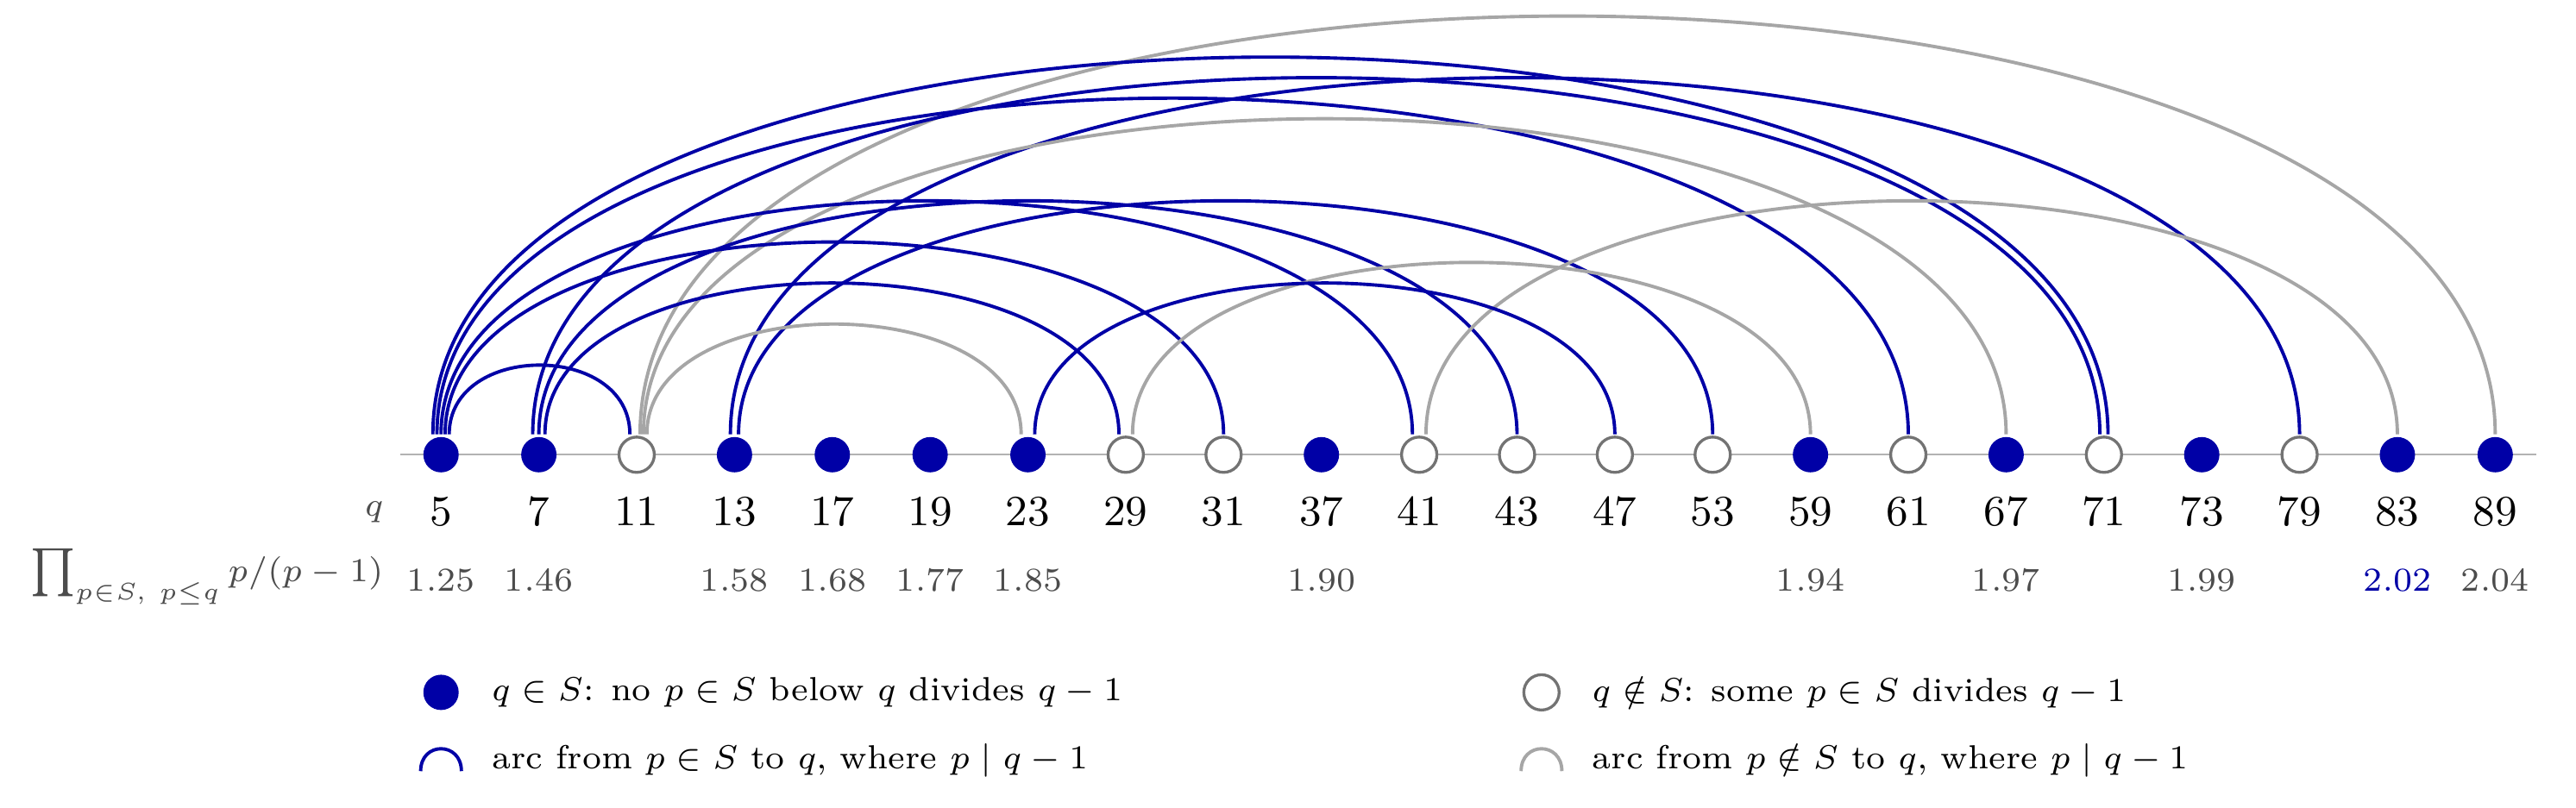
\includegraphics[width=\textwidth]{figures/fig_indep.png}
\caption{The primes from $5$ to $89$, with an arc from $p$ to $q$
whenever $p$ divides $q-1$; an independent set contains no two primes
joined by an arc. The set $S$ of filled primes is chosen one prime at
a time, each the least prime joined to none of those chosen before it.
Below each prime of $S$ is the product of $p/(p-1)$ over the primes of
$S$ up to it, which first exceeds $2$ at $83$, the eleventh.}
\label{fig:indep}
\end{figure}

\begin{proposition}\label{prop:indep}
\begin{enumerate}[label=\textup{(\roman*)}]
\item No independent set of at most $16000$ primes $p\ge5$ has
  $\prod p/(p-1)\ge2.999999$.
\item No independent set of at most $10^8$ primes $p\equiv2\pmod3$
  with $p\ge5$ has $\prod p/(p-1)\ge\frac83\bigl(1-10^{-6}\bigr)$.
\item No independent set of at most $10^8$ primes $p\equiv2\pmod3$
  with $p\ge5$ has $\prod p/(p-1)\ge\frac{10}3\bigl(1-10^{-6}\bigr)$.
\end{enumerate}
\end{proposition}

\begin{proof}
Let $Q$ be the set of primes allowed, $K$ the size and $V$ the target.
For an independent set $S\subseteq Q$ whose largest element is $p$
(with $p=3$ if $S$ is empty), call the primes $q\in Q$ with $q>p$ and
$q\not\equiv1$ modulo every element of $S$ the \emph{candidates} for
$S$. If $|S|<K$, let $B(S)$ be the product of $q/(q-1)$ over $S$ and
over the $K-|S|$ smallest candidates for $S$. An independent set $T$
of at most $K$ primes of $Q$ whose $|S|$ smallest elements form $S$
has its other elements among the candidates for $S$, and there are at
most $K-|S|$ of them; as $q/(q-1)$ decreases in $q$, the product over
$T$ is at most $B(S)$.

The search starts from the empty set and treats each set $S$ that it
creates as follows. If the product over $S$ is at least $V$, it stops
and reports $S$. If $|S|=K$ or $B(S)<V$, it discards $S$. Otherwise it
creates the sets $S\cup\{q\}$ for the candidates $q$ with
\begin{equation}\label{eq:childbound}
  \prod_{p\in S}\frac{p}{p-1}\cdot\frac{q}{q-1}\cdot
  \prod_{q'}\frac{q'}{q'-1}\ \ge\ V ,
\end{equation}
where $q'$ runs over the $K-|S|-1$ candidates for $S$ that follow $q$.
The left-hand side of \eqref{eq:childbound} is at least
$B(S\cup\{q\})$, because every candidate for $S\cup\{q\}$ is a
candidate for $S$, and it decreases as $q$ increases, so the sets
created from $S$ come from its first few candidates. Let $T$ be as
above with product at least $V$. Every initial segment $S$ of $T$ has
$B(S)\ge V$, and if $S\cup\{q\}$ is also an initial segment, then $q$
satisfies \eqref{eq:childbound}; so the search creates the initial
segments of $T$ one after another until it stops.

In each of the three cases the search ends without reporting a set. It
creates $90320$ sets in case (i), the largest of them with $46$
elements, and $9$ sets in case (ii) and $2$ in case (iii). Two programs
written independently, one of them in PARI/GP \cite{PARI}, carry out
the three searches and create the same sets. For (ii) and (iii), which
involve primes up to $2\cdot10^{10}$, they run through the primes once
for each set created. The products are handled through their
logarithms, and every bound is a sum of a few terms
$\log\bigl(q/(q-1)\bigr)$ and a difference of two running sums of
such terms. Every running sum here stays below $4$; it has fewer than
$2\cdot10^6$ terms in case (i), where the primes below $3\cdot10^7$
suffice, and fewer than $1.1\cdot10^8$ in cases (ii) and (iii). In
double precision each term is computed with an absolute error below
$3\cdot10^{-16}$ and each addition with one below $2^{-52}$, so a
bound carries an error below $10^{-8}$ in case (i) and below
$2\cdot10^{-7}$ in cases (ii) and (iii). The PARI/GP programs work
with $57$ significant digits in case (i) and $38$ in cases (ii) and
(iii), and their errors are below $10^{-45}$ and $10^{-25}$. A set is
discarded, or a candidate passed over, only when exact rational
arithmetic confirms it or when the logarithm of its bound lies below
$\log V$ by more than a margin that exceeds these errors: $10^{-7}$
in case (i) and $10^{-6}$ in cases (ii) and (iii) in double
precision, and $10^{-40}$ and $10^{-20}$ in PARI/GP. Rounding can
therefore add sets to the search, but never remove one.
\end{proof}

The search for (i) grows quickly with $K$: it creates $2567$ sets for
$K=10^4$ and $19711$ for $K=14000$. The least size of an independent
set of primes from $5$ on with product at least $3$ therefore lies
between $16001$ and $100470$, the length of the set chosen one prime
at a time above. For the primes $p\equiv2\pmod3$ the products grow
much more slowly: the independent set chosen from them in the same way
has $2307386$ elements below $2\cdot10^8$, and its product is only
$2.0703\ldots$, far below $\frac83$.

\begin{corollary}\label{cor:indep}
Let $n$ be as in Lemma~\ref{lem:basic}, with $M=(n+\varepsilon)/\varphi(n)$.
\begin{enumerate}[label=\textup{(\roman*)}]
\item If $M\ge3$ and $3\nmid n$, then $\omega(n)\ge16001$.
\item If $3\mid n$ and $\varepsilon=-1$, then $\omega(n)\ge10^8+2$.
\item If $3\mid n$, $\varepsilon=+1$ and $M\ge3$, then
  $\omega(n)\ge10^8+2$.
\end{enumerate}
\end{corollary}

\begin{proof}
Let $k=\omega(n)$. By Lemma~\ref{lem:basic} the prime factors of $n$
form an independent set, and $n/\varphi(n)=M-\varepsilon/\varphi(n)$.

(i) The prime factors are at least $5$, and
$n/\varphi(n)\ge3-1/\varphi(n)>2$. The product of $p/(p-1)$ over the
six smallest primes from $5$ on is $1.9490\ldots$, so $k\ge7$ and
$\varphi(n)\ge4\cdot6\cdot10\cdot12\cdot16\cdot18\cdot22>10^6$. Hence
$n/\varphi(n)>2.999999$, and Proposition~\ref{prop:indep}(i) gives
$k>16000$.

(ii) By Lemma~\ref{lem:three}, $M\ge4$, and the $k-1$ prime factors
other than $3$ are congruent to $2$ modulo $3$. The product of
$p/(p-1)$ over them is $\frac23\,n/\varphi(n)=\frac23(M+1/\varphi(n))>\frac83$,
so $k-1>10^8$ by Proposition~\ref{prop:indep}(ii).

(iii) By Lemma~\ref{lem:three}, $M\ge5$, and the prime factors other
than $3$ are as in (ii). The product over them is
$\frac23(M-1/\varphi(n))\ge\frac{10}3-\frac2{3\varphi(n)}\ge3$, while
over the five smallest primes $p\equiv2\pmod3$ from $5$ on it is
$1.5818\ldots$. So there are at least six of them,
$\varphi(n)\ge2\cdot4\cdot10\cdot16\cdot22\cdot28\cdot40>10^6$, and the
product exceeds $\frac{10}3(1-10^{-6})$. Proposition~\ref{prop:indep}(iii)
gives $k-1>10^8$.
\end{proof}

For $\varepsilon=-1$, part (ii) improves the bound $\omega(n)\ge40000000$
of Burcsi, Czirbusz and Farkas \cite{BCF11}, who completed sequences of
primes $p\equiv2\pmod3$ in a similar way by the least primes allowed.
Parts (i) and (iii) replace the bounds $33$ and $1540$ that the
products over the first primes give.

\begin{proof}[Proof of Theorem~\ref{thm:quotient} and of the last two
assertions of Theorem~\ref{thm:first}]
Let $n$ satisfy \eqref{eq:first} or \eqref{eq:second}, with $n$
composite in the first case and $n>3$ in the second. If $3\nmid n$ and
$M\ge3$, then $\omega(n)\ge16001$ by Corollary~\ref{cor:indep}(i). If
$3\mid n$, then $\omega(n)>10^8$ by Corollary~\ref{cor:indep}(ii) for
\eqref{eq:first}, where $M\ge4$ holds automatically, and by
Corollary~\ref{cor:indep}(iii) for \eqref{eq:second} when $M\ge3$.
\end{proof}

By Corollary~\ref{cor:indep}, a solution with at most $16000$ prime
factors has $M=2$, and if it solves \eqref{eq:first} it is prime to
$3$. The searches below concern the case $n+\varepsilon=2\varphi(n)$.

\begin{figure}[t]
\centering
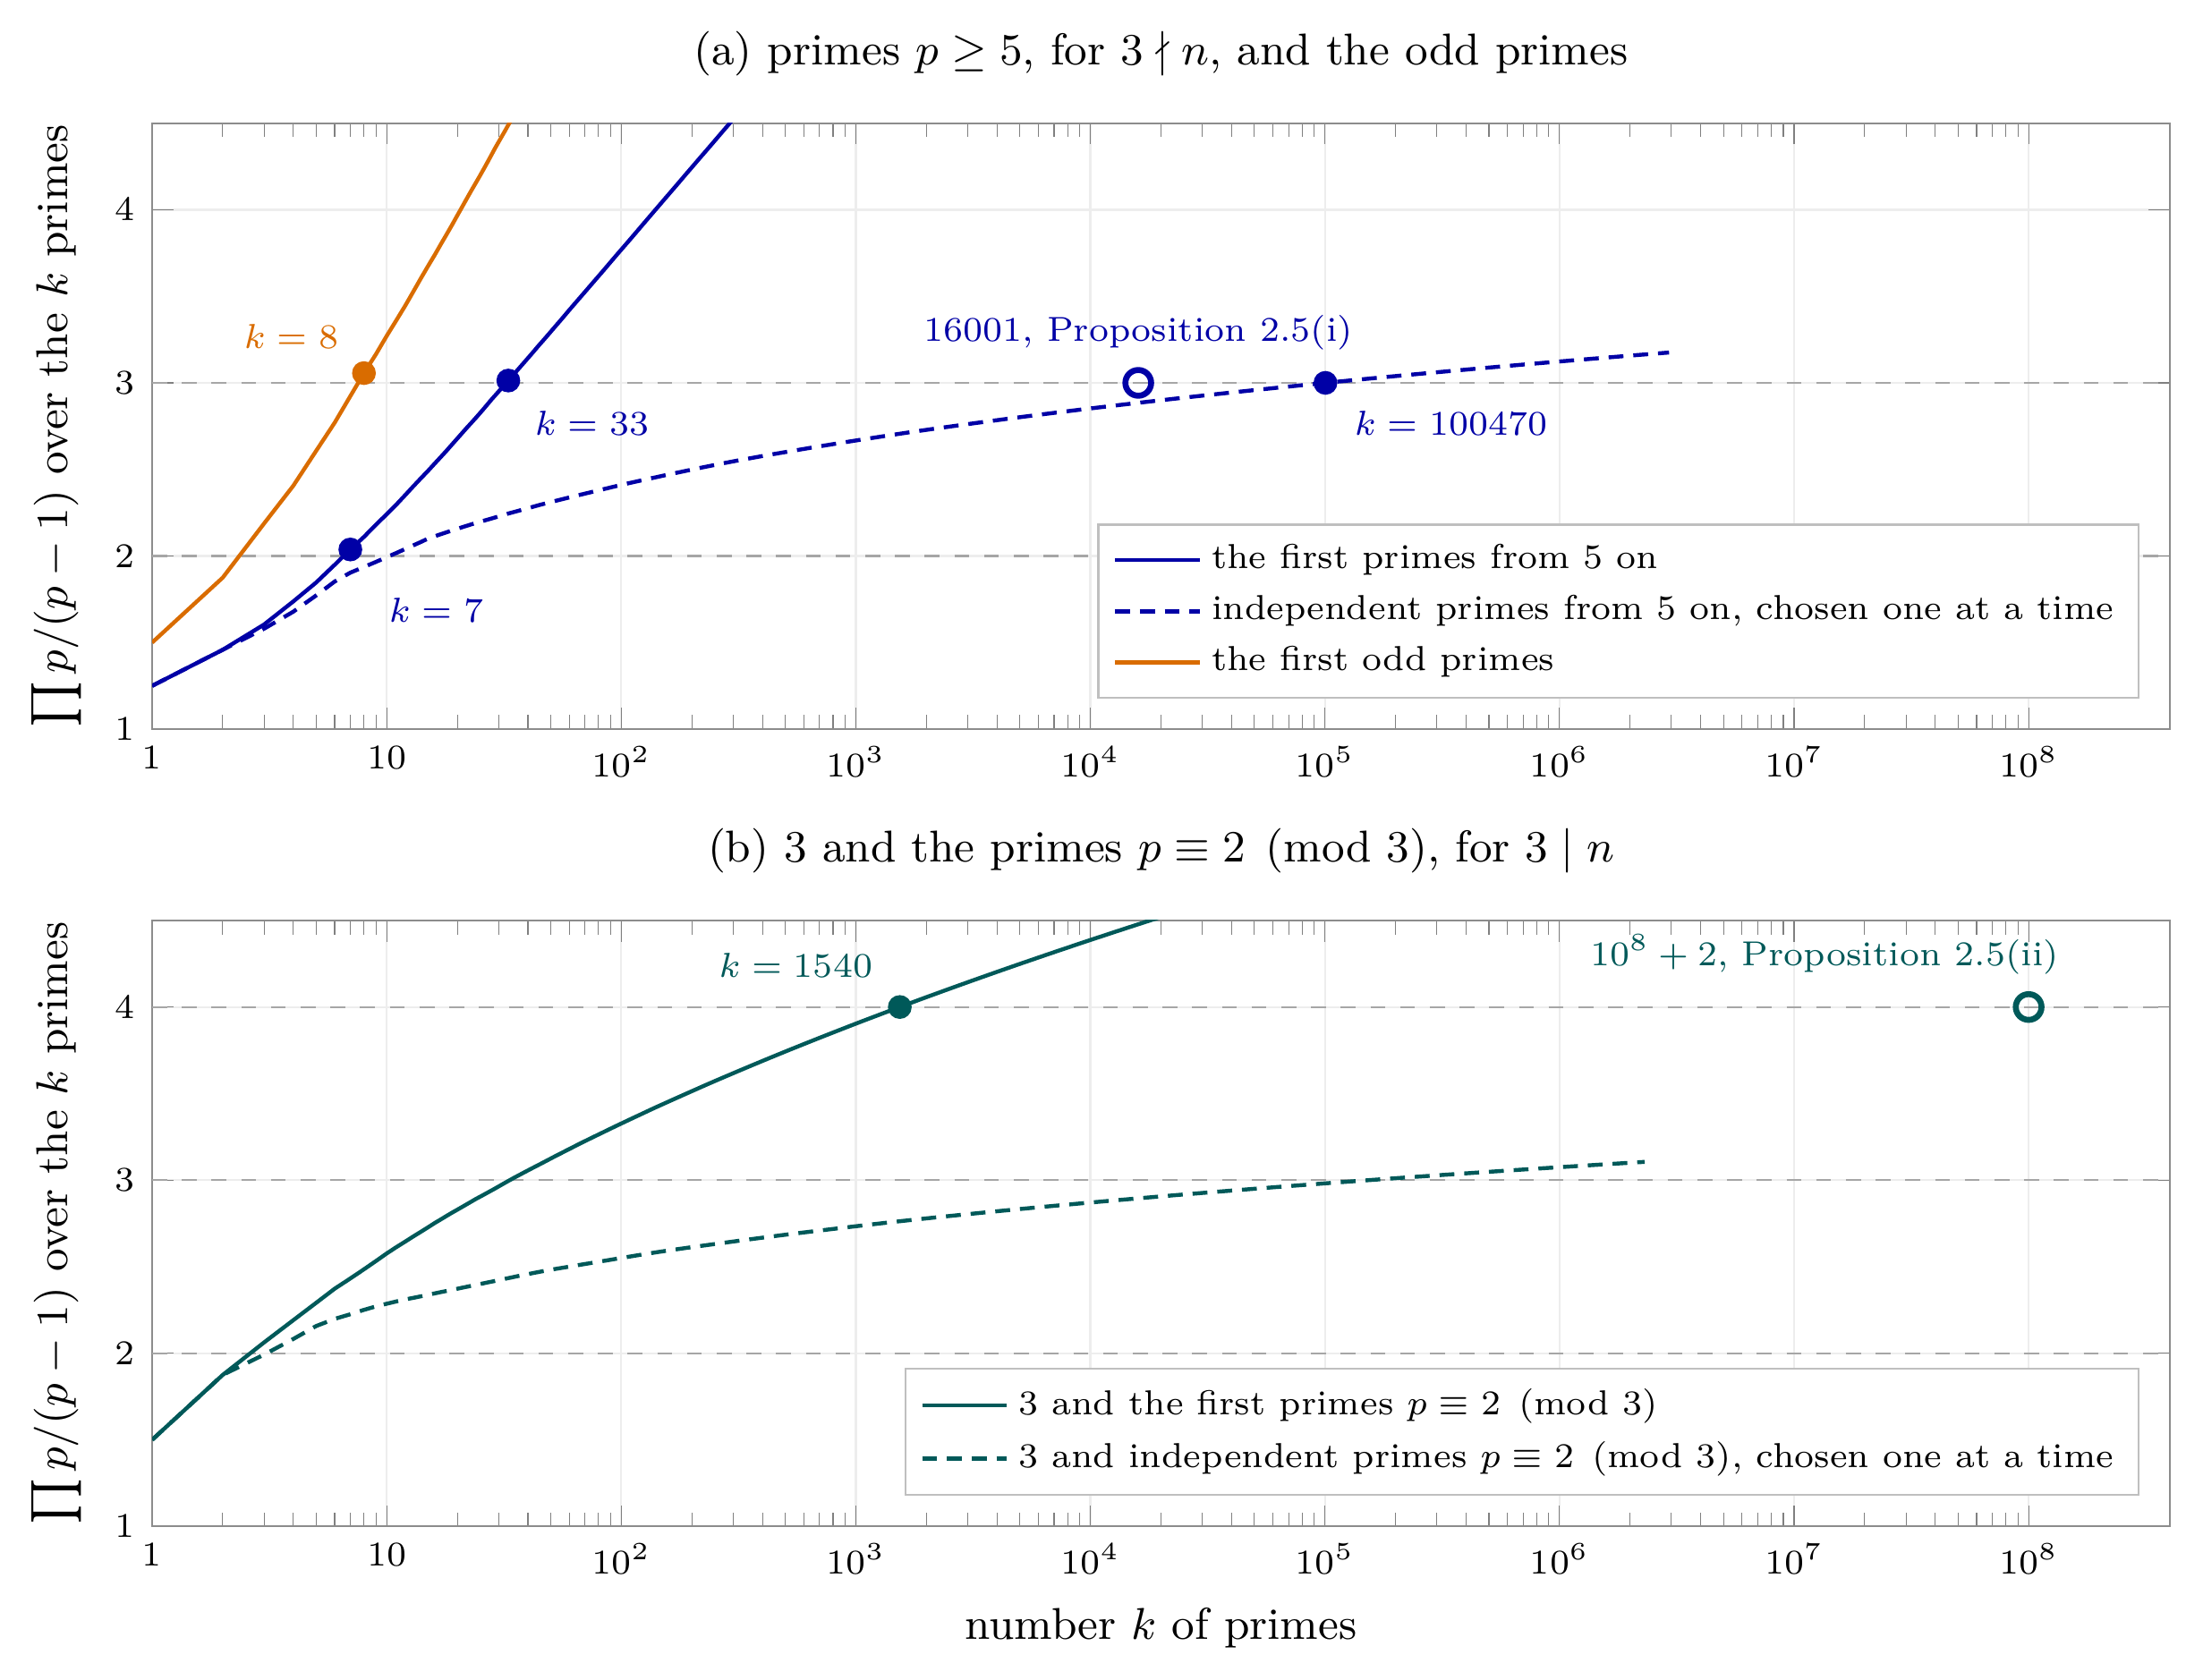
\includegraphics[width=0.9\textwidth]{figures/fig_products.png}
\caption{The product of $p/(p-1)$ over the first $k$ primes of a list
(solid) and over the independent set chosen from the same list one
prime at a time (dashed), for the primes below $2\cdot10^8$, with $k$ on
a logarithmic scale. Where a list has both curves, the largest product
over an independent set of $k$ of its primes lies between them. (a)~For
the primes from $5$ on the product passes $2$ at $k=7$, so a solution of
\eqref{eq:M2} prime to $3$ has at least seven prime factors
(Section~\ref{sec:first}), and $3$ at $k=33$ (Lemma~\ref{lem:Mtwo});
for the odd primes it passes $3$ at $k=8$, where the argument of
Corollary~\ref{cor:seven} stops. The independent set passes $3$ only at
$k=100470$, and no independent set of primes from $5$ on reaches $3$
before $k=16001$ (open circle). (b)~For $3$ and the primes
$p\equiv2\pmod3$ the product passes $4$ at $k=1540$
(Lemma~\ref{lem:three}), and no independent set formed by $3$ and such
primes reaches $4$ before $k=10^8+2$ (open circle).}
\label{fig:products}
\end{figure}

\subsection{The growth of independent sets}\label{sec:growth}
Proposition~\ref{prop:indep} needs a search because the product of
$p/(p-1)$ over an independent set grows very slowly with the size of
the set. Over the first $K$ primes the product is asymptotic to
$e^{\gamma}\log K$ by Mertens' theorem, so that the products alone
give only $\omega(n)\ge\exp(c'M)$ for some $c'>0$. Over an independent
set of $K$ primes the product is at most a constant multiple of
$\log\log K$, and this forces $\omega(n)$ to be at least doubly
exponential in $M$ (Theorem~\ref{thm:doubly}).

For a set $S$ of primes and $x\ge2$ put
\[
  P_S(x)=\prod_{p\in S,\ p\le x}\frac p{p-1},\qquad
  \delta_S(x)=\prod_{p\in S,\ p\le x}\Bigl(1-\frac1{p-1}\Bigr).
\]
An independent set with at least two elements does not contain $2$,
since $2$ divides $q-1$ for every odd prime $q$. For a set $S$ of odd
primes every factor of $\delta_S(x)$ is at least $\frac12$, and since
$\frac p{p-1}\bigl(1-\frac1{p-1}\bigr)=1-\frac1{(p-1)^2}$,
\begin{equation}\label{eq:deltaP}
  \delta_S(x)\,P_S(x)\le1 .
\end{equation}

\begin{theorem}\label{thm:sieve}
There is an absolute constant $c_0$ such that every independent set
$S$ of $K\ge3$ primes satisfies
\[
  \prod_{p\in S}\frac p{p-1}\le c_0\log\log K .
\]
\end{theorem}

The proof rests on the large sieve. Each element $p$ of $S$ excludes
from $S$ the primes congruent to $1$ modulo $p$, so that a prime above
$x$ can belong to $S$ only if it avoids one residue class modulo every
element of $S$ up to $x$; the large sieve bounds the number of such
primes by $\delta_S(x)$ times the number of all primes in the range.

\begin{lemma}\label{lem:sievestep}
Let $S$ be an independent set of odd primes and $N\ge2^{88}$. Then
\[
  \#\{q\in S:\ N^{1/44}<q\le N\}\le\frac{132\,N\,\delta_S(N^{1/44})}{\log N}.
\]
\end{lemma}

\begin{proof}
Put $Q=N^{1/2}$ and $z=N^{1/44}=Q^{1/22}$, so that $z\ge4$. For a prime
$p\le z$ let $\Omega_p$ consist of the residue class $0$ modulo $p$
and, if $p\in S$, also of the class $1$; for $z<p\le Q$ let $\Omega_p$
be empty. Let $\omega(p)<p$ be the number of classes in $\Omega_p$. A
prime $q\in S$ with $z<q\le N$ lies in none of these classes: it is
not divisible by a prime $p\le z<q$, and for $p\in S$ it is not
congruent to $1$ modulo $p$, because $S$ is independent. The large
sieve \cite{Mon68,MV73} states that a set of integers in $[1,N]$ that
avoids the classes of $\Omega_p$ for every prime $p\le Q$ has at most
$(N+Q^2)/L$ elements, where
\[
  L=\sum_{q\le Q}\mu^2(q)\,G(q),\qquad G(q)=\prod_{p\mid q}g(p),\qquad
  g(p)=\frac{\omega(p)}{p-\omega(p)} .
\]
Here $g(p)=1/(p-1)$ for $p\le z$ with $p\notin S$, $g(p)=2/(p-2)$ for
$p\le z$ with $p\in S$, and $g(p)=0$ for $p>z$; in every case
$g(p)\le6/p$.

Let $\Pi$ be the product of the primes up to $z$ and put
$\sigma=1/\log z$, so that $Q^{\sigma}=e^{22}$. Then $L$ is the sum of
$G(q)$ over the divisors $q\le Q$ of $\Pi$. A divisor $q>Q$ has
$(q/Q)^{\sigma}>1$, and so
\[
  \sum_{q\mid\Pi,\ q>Q}G(q)\le Q^{-\sigma}\sum_{q\mid\Pi}G(q)\,q^{\sigma}
  =e^{-22}\prod_{p\le z}\bigl(1+g(p)p^{\sigma}\bigr).
\]
For $p\le z$ we have $0<\sigma\log p\le1$, hence
$p^{\sigma}-1\le(e-1)\sigma\log p$ by convexity, and
$1+g(p)p^{\sigma}\le\bigl(1+g(p)\bigr)\exp\bigl(g(p)(p^{\sigma}-1)\bigr)$.
With $g(p)\le6/p$ and the elementary bound\footnote{Let
$m=\lfloor z\rfloor$. Legendre's formula gives
$\log m!\ge\sum_{p\le m}\lfloor m/p\rfloor\log p
>m\sum_{p\le m}(\log p)/p-\sum_{p\le m}\log p$, while
$\log m!\le m\log m$ and $\sum_{p\le m}\log p<m\log4$, because the
product of the primes up to $m$ is less than $4^m$. Dividing by $m$
gives the bound.}
$\sum_{p\le z}(\log p)/p<\log z+\log4$ this gives
\[
  \prod_{p\le z}\bigl(1+g(p)p^{\sigma}\bigr)
  \le\exp\Bigl(6(e-1)\Bigl(1+\frac{\log4}{\log z}\Bigr)\Bigr)
  \prod_{p\le z}\bigl(1+g(p)\bigr)
  <e^{20.7}\prod_{p\le z}\bigl(1+g(p)\bigr),
\]
because $z\ge4$ and $12(e-1)<20.7$. Since
$\prod_{p\le z}(1+g(p))=\sum_{q\mid\Pi}G(q)$ and $e^{20.7-22}<\frac13$,
the divisors $q>Q$ contribute less than a third of this sum, and
$L>\frac23\prod_{p\le z}(1+g(p))$. Finally $1+g(p)=p/(p-1)$ for
$p\notin S$ and $1+g(p)=\frac p{p-1}\bigl(1-\frac1{p-1}\bigr)^{-1}$ for
$p\in S$, so that
\[
  \prod_{p\le z}\bigl(1+g(p)\bigr)
  =\frac1{\delta_S(z)}\prod_{p\le z}\Bigl(1-\frac1p\Bigr)^{-1}
  >\frac{\log z}{\delta_S(z)},
\]
since the product $\prod_{p\le z}(1-1/p)^{-1}$ is at least
$\sum_{n\le z}1/n>\log z$. With $\log z=(\log N)/44$ we obtain
$L>\log N/(66\,\delta_S(z))$, and the large sieve, with $N+Q^2=2N$,
gives the lemma.
\end{proof}

\begin{lemma}\label{lem:sievesum}
Let $S$ be an independent set of odd primes and $y\ge2^{88}$. Then
\[
  \sum_{q\in S,\ y<q\le y^2}\frac1q\le269\,\delta_S\bigl(y^{1/44}\bigr).
\]
\end{lemma}

\begin{proof}
Let $a=\lfloor\log_2y\rfloor\ge88$ and $b=\lceil2\log_2y\rceil$, so
that $b\le2a+2$. The interval $(y,y^2]$ is covered by the intervals
$(2^{i-1},2^i]$ with $a<i\le b$. For each such $i$,
Lemma~\ref{lem:sievestep} with $N=2^i$ applies to the elements of $S$
in $(2^{i-1},2^i]$, because $2^{i/44}\le2^{i-1}$, and
$\delta_S(2^{i/44})\le\delta_S(y^{1/44})$, because $2^i>y$ and
$\delta_S$ is decreasing. Each of these elements exceeds $2^{i-1}$, so
their reciprocals add up to at most
\[
  \frac{132\cdot2^i\,\delta_S(y^{1/44})}{2^{i-1}\,i\log2}
  =\frac{264\,\delta_S(y^{1/44})}{i\log2}.
\]
Since $\sum_{a<i\le b}1/i\le\log(b/a)\le\log(2+2/88)<0.705$ and
$264\cdot0.705/\log2<269$, the lemma follows.
\end{proof}

\begin{proof}[Proof of Theorem~\ref{thm:sieve}]
By Mertens' theorem $\prod_{p\le x}(1-1/p)^{-1}=e^{\gamma}\log x+O(1)$,
so there is an absolute constant $c_1$ with
$\prod_{u<p\le u^{44}}p/(p-1)\le c_1$ for all $u\ge2$. Let $S$ be an
independent set of odd primes. Then $P_S(y)\le c_1P_S(y^{1/44})$ for
$y\ge2^{44}$, and
Lemma~\ref{lem:sievesum} and \eqref{eq:deltaP} give, for $y\ge2^{88}$,
\begin{equation}\label{eq:sievestep}
  \sum_{q\in S,\ y<q\le y^2}\frac1q\le\frac{269}{P_S(y^{1/44})}
  \le\frac{269\,c_1}{P_S(y)} .
\end{equation}
Put $y_0=2^{88}$, $y_{j+1}=y_j^2$ and $a_j=P_S(y_j)$. Since
$-\log(1-1/q)\le2/q$, \eqref{eq:sievestep} gives
$a_{j+1}\le a_je^{c_2/a_j}$ with $c_2=538\,c_1$, and also
$a_{j+1}\le c_1a_j$. If $a_j\ge c_2$, then
$a_{j+1}\le a_j(1+2c_2/a_j)=a_j+2c_2$, because $e^t\le1+2t$ for
$0\le t\le1$; if $a_j<c_2$, then $a_{j+1}<c_1c_2$. By induction
$a_j\le c_3+2c_2j$ for all $j\ge0$, where
$c_3=\max\bigl\{c_1c_2,\prod_{p\le2^{88}}p/(p-1)\bigr\}\ge a_0$. For $x>y_0$
let $j$ be the least index with $y_j\ge x$. Then
$2^{j-1}\log y_0<\log x$, and
$P_S(x)\le a_j\le c_3+2c_2\bigl(1+\log_2(\log x/\log y_0)\bigr)$.
Together with $P_S(x)\le a_0\le c_3$ for $x\le y_0$, this gives
$P_S(x)\le c_4\log\log x$ for all $x\ge3$, with an absolute constant
$c_4$.

Now let $S$ have $K\ge3$ elements, so that its elements are odd. At
most $K$ of them exceed $K^2$, and each of those contributes a factor
at most $1+1/K^2$, so that together they contribute less than
$e^{1/K}<2$. Hence
\[
  \prod_{p\in S}\frac p{p-1}<2P_S(K^2)\le2c_4\log\log K^2
  =2c_4(\log2+\log\log K)\le20\,c_4\log\log K,
\]
since $\log2<9\log\log3$.
\end{proof}

\begin{proof}[Proof of Theorem~\ref{thm:doubly}]
Let $n$ be as in Lemma~\ref{lem:basic} and $k=\omega(n)\ge2$. The prime
factors of $n$ form an independent set, and $n/\varphi(n)$ is the
product of $p/(p-1)$ over them. If $k\ge3$, Theorem~\ref{thm:sieve} and
Lemma~\ref{lem:basic}(iii) give
$M\le c_0\log\log k+1/\varphi(n)<(c_0+3)\log\log(k+2)$, since
$\log\log5>\frac13$. If $k=2$, then $n/\varphi(n)\le\frac32\cdot\frac54$
and $\varphi(n)\ge8$, so that $M\le2<7\log\log4$. In both cases
$\log\log(k+2)\ge cM$ with $c=1/\max\{c_0+3,7\}$, which is the
assertion.
\end{proof}

The constants in Theorems~\ref{thm:sieve} and~\ref{thm:doubly} are
effective but large, and the numerical bounds of
Corollary~\ref{cor:indep} come from Proposition~\ref{prop:indep}, not
from the sieve. What the sieve explains is the shape of those bounds.
Heuristically, the elements of $S$ up to $x$ leave a proportion
$\delta_S(x)$ of the primes near $x$ available, and a set that takes
every available prime gains $\log P_S$ at the rate
$\delta_S(x)\,d\log\log x$, since $\sum_{q\le x}1/q$ grows like
$\log\log x$. The derivative of $P_S$ with respect to $\log\log x$ is
then $\delta_S(x)P_S(x)$, which is at most $1$ by \eqref{eq:deltaP},
so that $P_S(x)$ grows at most like $\log\log x$, the rate of
Theorem~\ref{thm:sieve}. The independent sets chosen one prime at a
time in Section~\ref{sec:indep} grow at this rate
(Table~\ref{tab:greedy}). Between $x=10^3$ and $x=10^8$ the product of
$p/(p-1)$ over the elements up to $x$ differs from a linear function of
$\log\log x$ by less than $0.003$, with slope $0.82$ for the primes
from $5$ on and $0.41$ for the primes $p\equiv2\pmod3$, which are
half of all primes. The first set needs $100470$ primes to reach the
product $3$, where the first primes from $5$ on need $33$, and the
second has not reached $\frac83$ below $2\cdot10^8$
(Section~\ref{sec:indep}). This is
why the bounds of Corollary~\ref{cor:indep} exceed $33$ and $1540$ by
so much.

\begin{table}[ht]
\centering
\caption{The independent sets chosen one prime at a time from the
primes from $5$ on and from the primes $p\equiv2\pmod3$ from $5$ on:
the number of elements up to $x$ and the product of $p/(p-1)$ over
them.}
\label{tab:greedy}
\smallskip
\small
\begin{tabular}{@{}rrrrrr@{}}
\toprule
 & & \multicolumn{2}{c}{primes from $5$ on} &
 \multicolumn{2}{c}{$p\equiv2\pmod3$} \\
\cmidrule(lr){3-4}\cmidrule(l){5-6}
$x$ & $\log\log x$ & elements & product & elements & product \\
\midrule
$10^3$ & $1.933$ & $62$ & $2.3430$ & $45$ & $1.6489$ \\
$10^4$ & $2.220$ & $407$ & $2.5792$ & $293$ & $1.7626$ \\
$10^5$ & $2.443$ & $2\,908$ & $2.7593$ & $2\,185$ & $1.8564$ \\
$10^6$ & $2.626$ & $22\,602$ & $2.9078$ & $17\,396$ & $1.9328$ \\
$10^7$ & $2.780$ & $183\,730$ & $3.0344$ & $142\,723$ & $1.9979$ \\
$10^8$ & $2.913$ & $1\,538\,281$ & $3.1447$ & $1\,207\,989$ & $2.0546$ \\
\bottomrule
\end{tabular}
\end{table}

%%==================================================================
\section{Intervals for the prime factors}\label{sec:search}
%%==================================================================

Fix $k\ge2$, a sign $\varepsilon$, and a squarefree odd
$n=p_1\cdots p_k$ with
\begin{equation}\label{eq:M2}
  n+\varepsilon=2\varphi(n).
\end{equation}
By Lemma~\ref{lem:basic}(iii),
\begin{equation}\label{eq:excess}
  \prod_{i=1}^{k}\frac{p_i}{p_i-1}=2-\frac{\varepsilon}{\varphi(n)} .
\end{equation}
For $\varepsilon=-1$ the product lies just above $2$, and for
$\varepsilon=+1$ just below it. Everything in this section is a
consequence of \eqref{eq:excess}, and the two signs are treated
together.

\begin{proposition}\label{prop:below2}
$P_j<2$ for every $j<k$.
\end{proposition}

\begin{proof}
For $\varepsilon=+1$ this is clear, since $P_j\le P_k=2-1/\varphi(n)$.
For $\varepsilon=-1$, suppose $P_j\ge2$ with $j<k$. Since
$p_{j+1}-1<n-1$ we have $p_{j+1}/(p_{j+1}-1)>1+1/(n-1)$, and the
remaining factors exceed $1$, so
$P_k>2\bigl(1+1/(n-1)\bigr)=2+1/\varphi(n)$ by \eqref{eq:M2},
contradicting \eqref{eq:excess}.
\end{proof}

At depth $j$ put $T=2/P_j$, which exceeds $1$ by the proposition, and
\[
  C_j=2B_j-A_j,\qquad T-1=\frac{C_j}{A_j}.
\]
Thus $C_j$ is a positive integer, and $C_j/A_j$ measures how far the
primes chosen so far fall short of the target $2$.

\begin{proposition}\label{prop:bounds}
Let $0\le j\le k-2$, $m=k-j$, $W=(p_j+1)^m$ and
$x=p_{j+1}/(p_{j+1}-1)$. Then
\begin{equation}\label{eq:bounds}
\begin{aligned}
  &x^m>T \quad\text{and}\quad x<T+\frac{1}{A_jW} &&\text{if }\varepsilon=-1,\\
  &x^m\ge T-\frac{1}{A_jW}\quad\text{and}\quad x<T &&\text{if }\varepsilon=+1 .
\end{aligned}
\end{equation}
In particular $p_{j+1}$ lies in an interval $[L_j,U_j]$ whose
endpoints are determined by $p_1,\dots,p_j$, $k$ and $\varepsilon$.
\end{proposition}

\begin{proof}
Let $\rho=\prod_{i>j}p_i/(p_i-1)$. By \eqref{eq:excess},
\[
  \rho=\frac{2-\varepsilon/\varphi(n)}{P_j}
  =T-\frac{\varepsilon}{P_j\varphi(n)} .
\]
There are $m\ge2$ factors in $\rho$; each exceeds $1$ and none exceeds
$x$, because $p/(p-1)$ decreases in $p$. Hence $x<\rho\le x^m$. The
remaining primes are odd and larger than $p_j$ (larger than $2$ when
$j=0$), so $p_i-1\ge p_j+1$ for $i>j$, and
$\varphi(n)=B_j\prod_{i>j}(p_i-1)\ge B_jW$. Therefore
\[
  0<\frac{1}{P_j\varphi(n)}\le\frac{1}{P_jB_jW}=\frac1{A_jW},
\]
and the four inequalities follow from $x<\rho\le x^m$. Finally, for
$\varepsilon=+1$ the quantity $T-1/(A_jW)$ exceeds $1$, since
$T-1=C_j/A_j\ge1/A_j$.
\end{proof}

Apart from the correction terms, \eqref{eq:bounds} says $x<T\le x^m$,
that is $1/(T-1)<p_{j+1}-1\le1/(T^{1/m}-1)$. Since
$T^{1/m}-1$ is close to $(T-1)/m$, the interval has length about
$(m-1)/(T-1)=(m-1)A_j/C_j$ (Figure~\ref{fig:interval}). The upper end
obeys a bound that makes the search finite.

\begin{corollary}\label{cor:finite}
Let $0\le j\le k-2$, let $p_1<\dots<p_j$ be odd primes with $P_j<2$,
and let $p_{j+1}>p_j$ be a prime that satisfies the inequality for
$x^m$ in \eqref{eq:bounds}. Then $p_{j+1}<1+3(k-j)B_j/C_j<4kA_j$. If
$n=p_1\cdots p_k$ satisfies \eqref{eq:M2}, then moreover
$p_k\le2B_{k-1}+1$, and
\[
  A_j<(4k)^{2^j}\quad(0\le j\le k),\qquad n<(4k)^{2^k}.
\]
\end{corollary}

\begin{proof}
Let $m=k-j$ and $x=p_{j+1}/(p_{j+1}-1)$, so that
$p_{j+1}-1=1/(x-1)$. By \eqref{eq:bounds}, $x^m\ge T'$, where $T'=T$
if $\varepsilon=-1$ and $T'=T-1/(A_jW)$ if $\varepsilon=+1$. As
$T-1=C_j/A_j$ with $C_j\ge1$, and $W\ge4$, in both cases
$T'-1\ge(C_j-\frac14)/A_j\ge3C_j/(4A_j)>0$ and $T'\le T$. For $t>1$
we have $t^{1/m}-1=(t-1)/\sum_{i<m}t^{i/m}\ge(t-1)/(mt)$, and so
\[
  p_{j+1}-1=\frac1{x-1}\le\frac1{T'^{1/m}-1}\le\frac{mT'}{T'-1}
  \le\frac{2mB_j}{A_j}\cdot\frac{4A_j}{3C_j}<\frac{3mB_j}{C_j}.
\]
Since $C_j\ge1$ and $B_j\le A_j-1$ for $j\ge1$, while
$A_0=B_0=C_0=1$, this gives $p_{j+1}<4kA_j$. For a solution, the
equation $A_{k-1}p_k+\varepsilon=2B_{k-1}(p_k-1)$ gives
$p_kC_{k-1}=2B_{k-1}+\varepsilon$, and $C_{k-1}\ge1$ by
Proposition~\ref{prop:below2}, so that $p_k\le2B_{k-1}+1<4kA_{k-1}$.
By Propositions~\ref{prop:below2} and~\ref{prop:bounds} the first part
applies to $p_{j+1}$ for every $j\le k-2$. Hence $A_{j+1}<4kA_j^2$ for
$0\le j<k$, and induction gives $A_j\le(4k)^{2^j-1}$.
\end{proof}

Every node of the search below satisfies the hypotheses of
Corollary~\ref{cor:finite}, so the tree has finitely many nodes and the
search terminates. The bound $n<(4k)^{2^k}$ has the shape of the bound
$n<k^{2^k}$ of Pomerance \cite{Pom77}; Theorem~\ref{thm:size} replaces
it by $n<2^{2^{k-7}}$.

\begin{figure}[t]
\centering
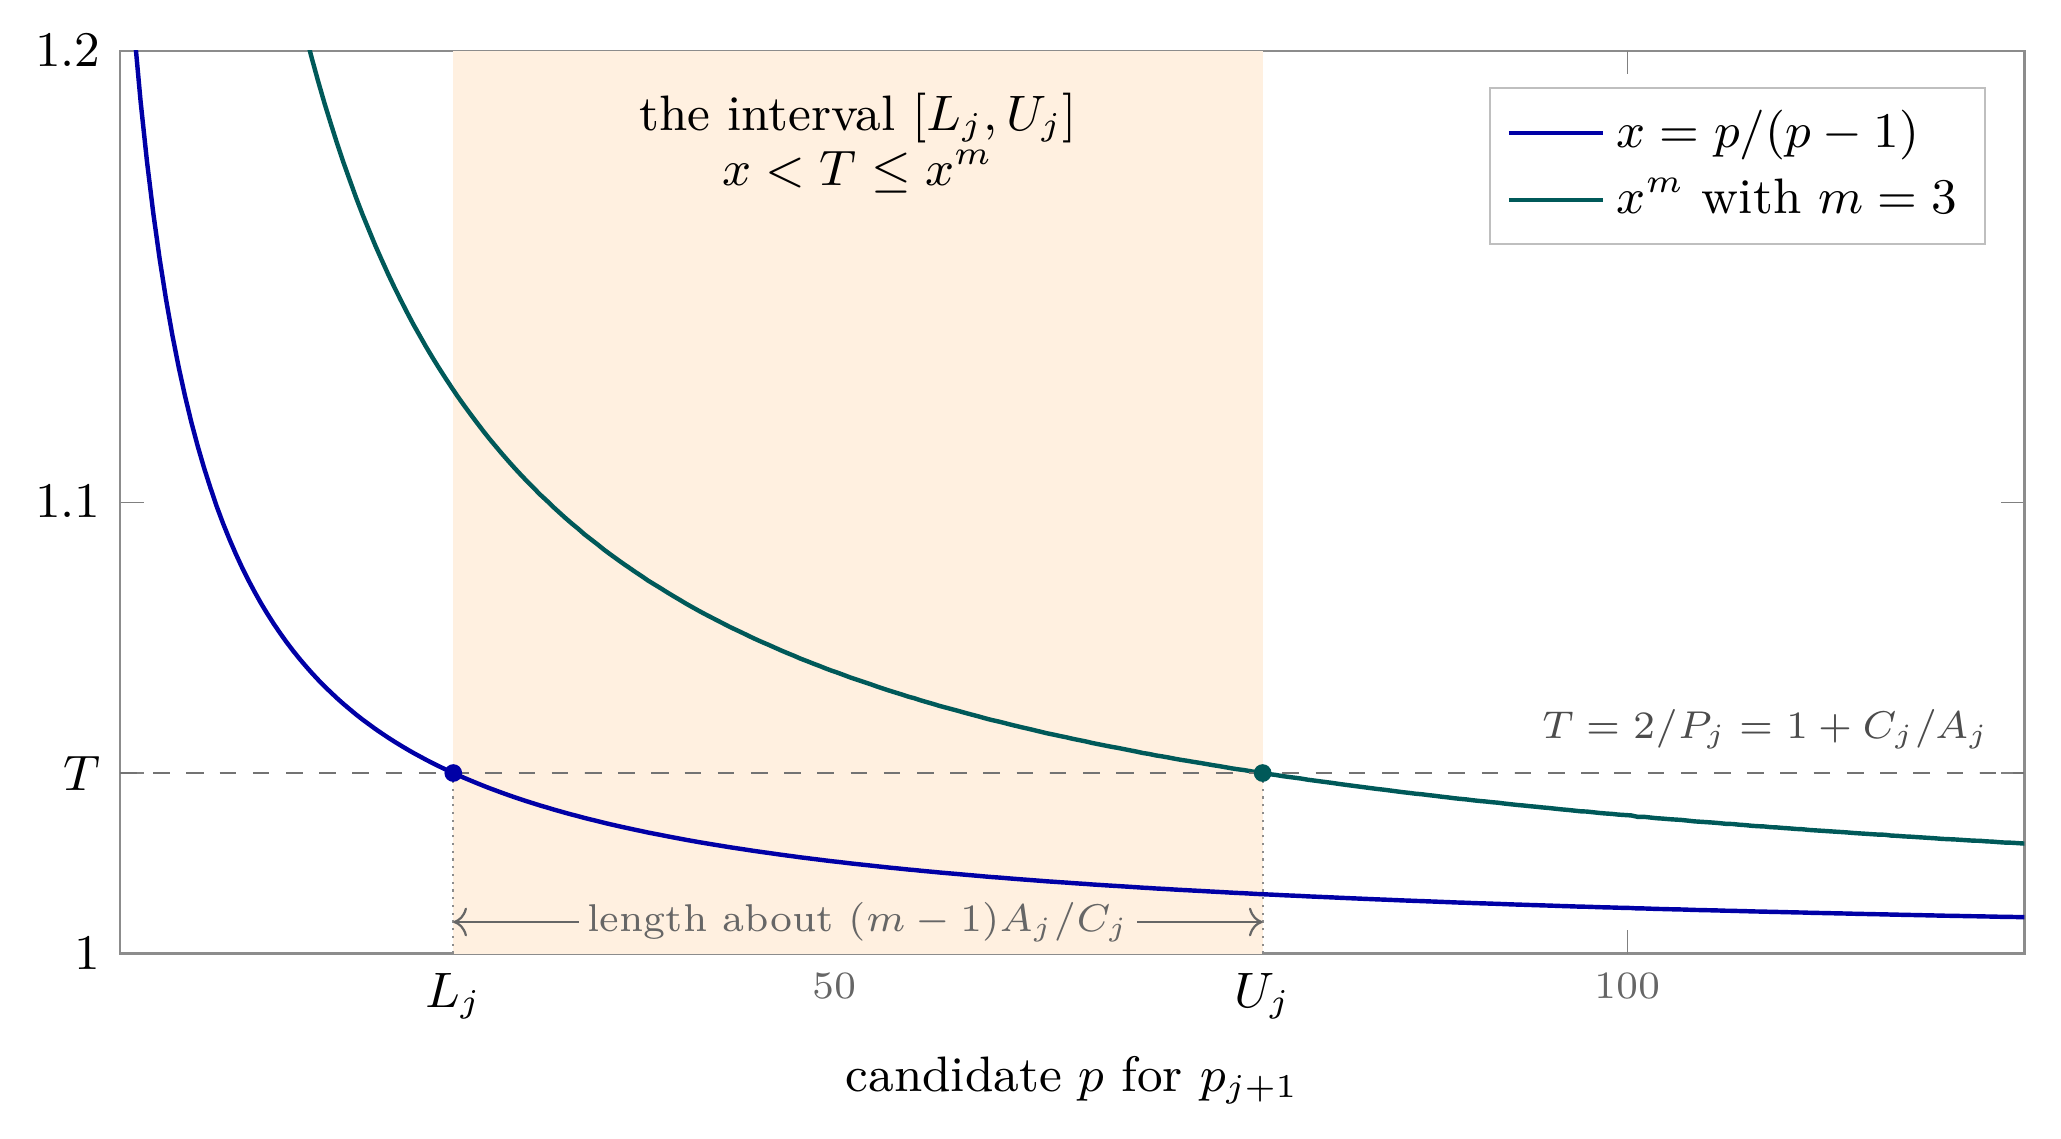
\includegraphics[width=0.86\textwidth]{figures/fig_interval.png}
\caption{The interval of Proposition~\ref{prop:bounds} for $T=1.04$
and $m=3$, with the correction terms $1/(A_jW)$ left out. The
candidate $p$ must satisfy $x<T$, because the other $m-1$ factors of
$\rho$ exceed $1$, and $x^m\ge T$, because none of them exceeds $x$.
Here the two conditions give $26<p<77$.}
\label{fig:interval}
\end{figure}

The inequalities \eqref{eq:bounds} are tested in integers: for instance
$x^m>T$ reads $p^mA_j>2B_j(p-1)^m$. A floating-point estimate is used
only to find a starting point, which is then corrected by exact
comparisons.

\begin{lemma}[congruence prune]\label{lem:prune}
No prime factor of $n$ divides $p-1$ for another prime factor $p$ of
$n$.
\end{lemma}

This is Lemma~\ref{lem:basic}(ii). A candidate $p$ for $p_{j+1}$ is
discarded if $p\mid p_i-1$ or $p_i\mid p-1$ for some $i\le j$. The
primes of the interval $[L_j,U_j]$ that are not discarded are called
\emph{admissible}.

The last two primes are determined together by a divisibility
condition.

\begin{proposition}\label{prop:last}
Let $A=A_{k-2}$, $B=B_{k-2}$, $C=2B-A$, $p=p_{k-1}$ and $q=p_k$. Then
\begin{equation}\label{eq:last}
  t:=Cp-2B>0,\qquad t\mid Ap+\varepsilon,\qquad
  q=1+\frac{Ap+\varepsilon}{t},
\end{equation}
and equivalently
\begin{equation}\label{eq:hyperbola}
  (Cp-2B)(Cq-2B)=2AB+\varepsilon C .
\end{equation}
\end{proposition}

\begin{proof}
Equation \eqref{eq:M2} reads $Apq+\varepsilon=2B(p-1)(q-1)$. Collecting
the terms in $q$ gives $q\,(Cp-2B)=2B(p-1)+\varepsilon$. The right-hand
side is positive, so $t>0$, and
$q-1=\bigl(2Bp-2B+\varepsilon-Cp+2B\bigr)/t=(Ap+\varepsilon)/t$.
Multiplying $Cpq-2B(p+q)+2B-\varepsilon=0$ by $C$ and completing the
product gives
$(Cp-2B)(Cq-2B)=4B^2-2BC+\varepsilon C=2AB+\varepsilon C$.
\end{proof}

Once $p_1,\dots,p_{k-2}$ are fixed, the prime $p_{k-1}$ runs over the
interval of Proposition~\ref{prop:bounds} with $m=2$, and for each
candidate $p$ the last prime is determined by \eqref{eq:last}.
Alternatively, by \eqref{eq:hyperbola}, $t$ is a divisor of the integer
\[
  D=2AB+\varepsilon C
\]
lying in a known residue class modulo $C$, so the candidates can be
read off from the divisors of $D$ when $D$ can be factored. The first
route costs time proportional to the length of the interval, the
second the cost of factoring $D$. Figure~\ref{fig:search} summarises
the procedure.

\begin{figure}[t]
\centering
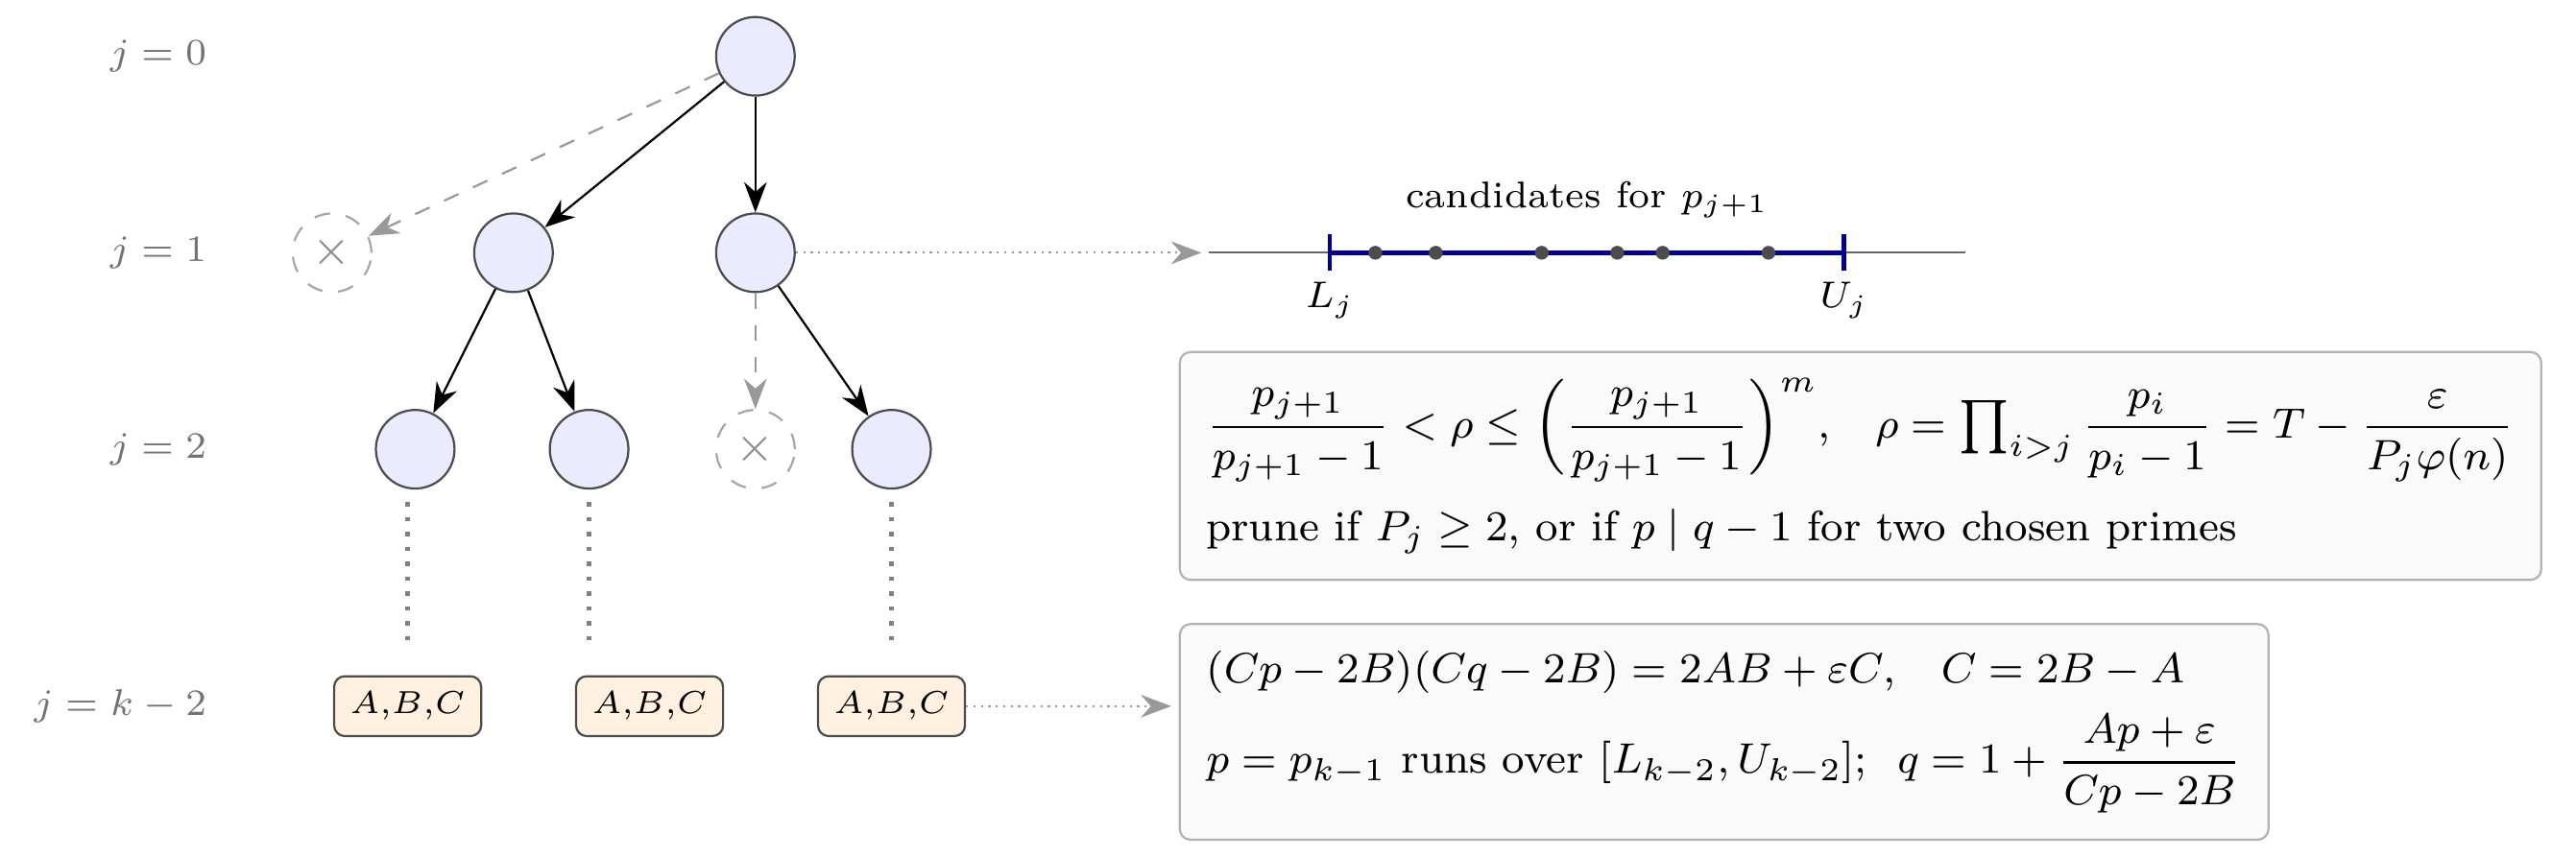
\includegraphics[width=\textwidth]{figures/fig_search.png}
\caption{The search for $n=p_1\cdots p_k$ with $n+\varepsilon=2\varphi(n)$.
A node at depth $j$ is an increasing sequence of primes
$p_1<\dots<p_j$. Its children are the primes in the interval
$[L_j,U_j]$ of Proposition~\ref{prop:bounds} that pass the congruence
prune; dashed branches are cut. At depth $k-2$ the pair
$(p_{k-1},p_k)$ is a lattice point on the hyperbola
\eqref{eq:hyperbola}, found by running $p$ over $[L_{k-2},U_{k-2}]$
or by factoring $2AB+\varepsilon C$.}
\label{fig:search}
\end{figure}

The search is a depth-first traversal of the tree whose nodes at depth
$j\le k-2$ are the increasing sequences $(p_1,\dots,p_j)$ of primes
with $p_1\ge p_{\min}$, where each $p_{i+1}$ lies in the interval
determined by $(p_1,\dots,p_i)$ and passes the congruence prune, and
where $P_i<2$ for all $i\le j$. At depth $k-2$ each candidate
$p_{k-1}$ is tested with \eqref{eq:last}: one checks that $t>0$, that
$t\mid Ap+\varepsilon$, that $q=1+(Ap+\varepsilon)/t$ is a prime larger
than $p$, that $p$ and $q$ pass the congruence prune, and finally that
\eqref{eq:M2} holds exactly.

\begin{theorem}[completeness]\label{thm:complete}
If $n=p_1\cdots p_k$ with primes $p_{\min}\le p_1<\dots<p_k$ satisfies
\eqref{eq:M2}, then the traversal visits $(p_1,\dots,p_{k-2})$,
examines the candidate $p_{k-1}$, and records $n$.
\end{theorem}

\begin{proof}
By induction on $j$ the node $(p_1,\dots,p_j)$ is visited for every
$j\le k-2$: the prime $p_{j+1}$ lies in the interval of
Proposition~\ref{prop:bounds}, it passes the prune by
Lemma~\ref{lem:prune}, and $P_{j+1}<2$ by
Proposition~\ref{prop:below2}. At depth $k-2$ the candidate
$p=p_{k-1}$ satisfies \eqref{eq:last} with $q=p_k$. A primality test
never declares a prime to be composite, so $q$ is accepted, and the
final check of \eqref{eq:M2} succeeds.
\end{proof}

The search is rigorous for two reasons. First, all arithmetic is
exact:
$A_j$, $B_j$, $C_j$, the interval endpoints and the quantities in
\eqref{eq:last} are integers or ratios of integers compared by cross
multiplication. Second, the probabilistic primality tests used by the
programs\footnote{Below the number
$\psi_{13}=3317044064679887385961981$ the programs use a strong
probable-prime test to the thirteen bases $2,3,\dots,41$, and above it
a Baillie--PSW test. Sorenson and Webster \cite{SW17} showed that
every composite number below $\psi_{13}$ fails the first test for at
least one of these bases, so there it is a proof. The
Baillie--PSW test \cite{BW80,PSW80} combines a strong probable-prime
test to base $2$ with a strong Lucas test; no composite number is
known to pass it.} can err only by declaring a composite number prime,
never by declaring a prime composite. Such an error could add a node
or accept a composite $q$, but it can never remove an actual solution.
A search that finds nothing is therefore a proof that there is
nothing, and the completeness of the enumeration route depends on no
primality proof. The exact check of \eqref{eq:M2} would not catch such
an error, since it uses $\prod(p_i-1)$ in place of $\varphi(n)$. This
matters only for solutions that are reported, and every solution
reported in this paper, including those of Appendix~\ref{app:known},
has all its prime factors below $10^{14}$, where the tests are
proofs. The divisor route depends on a complete
factorisation of $D$, which is certified whenever $D<\psi_{13}$,
since then every prime factor of $D$ lies below that bound.

%%==================================================================
\section{The last three primes}\label{sec:three}
%%==================================================================

For $k\le14$ the search of Section~\ref{sec:search} is cheap because
the interval for $p_{k-1}$ is never longer than about $5\cdot10^7$. For
$k=15$ this is no longer true. After the prime $p_{13}$ has been chosen
the interval for $p_{14}$ can be longer than $10^{14}$, and there are
tens of millions of choices of $p_{13}$. Neither route of
Section~\ref{sec:search} copes with this: running $p_{14}$ over its
interval is far too slow, and factoring tens of millions of integers of
about fifty digits is a computation of a different order. In this
section we describe two further ways of finding the divisors of
$2AB+\varepsilon C$ that can occur in Proposition~\ref{prop:last}.
Both use the residue class in which these divisors lie: the first
lists lattice points near a hyperbola, and the second scans the
possible values of the sum of two complementary divisors.

\subsection{Reduction to divisors in a residue class}
Fix a node $(p_1,\dots,p_{k-3})$ at depth $k-3$ and a candidate
$s=p_{k-2}$ in its interval that passes the congruence prune. Put
\[
  A'=A_{k-3}\,s,\qquad B'=B_{k-3}\,(s-1),\qquad c=2B'-A',\qquad
  N=2A'B'+\varepsilon c .
\]
If $c\le0$ then $P_{k-2}=A'/B'\ge2$, and by
Proposition~\ref{prop:below2} no solution has $p_1,\dots,p_{k-3},s$ as
its first $k-2$ primes; such $s$ are discarded. So let $c\ge1$. By
Proposition~\ref{prop:last}, applied with $A=A'$ and $B=B'$, the
remaining primes $p<q$ of a solution satisfy
$(cp-2B')(cq-2B')=N$ with both factors positive. Let $r$ be the least
positive residue of $-2B'$ modulo $c$.

By \eqref{eq:excess} the last three primes satisfy
\[
  \frac{s}{s-1}\cdot\frac{p}{p-1}\cdot\frac{q}{q-1}
  =T-\frac{\varepsilon}{P_{k-3}\,\varphi(n)},\qquad T=\frac{2}{P_{k-3}},
\]
so the point $(s,p,q)$ lies next to the surface on which this product
equals $T$. Fixing $s$ cuts the surface in a curve, and the pair
$(p,q)$ lies exactly on the hyperbola $(cp-2B')(cq-2B')=N$ beside that
curve (Figure~\ref{fig:surface}).

\begin{figure}[t]
\centering
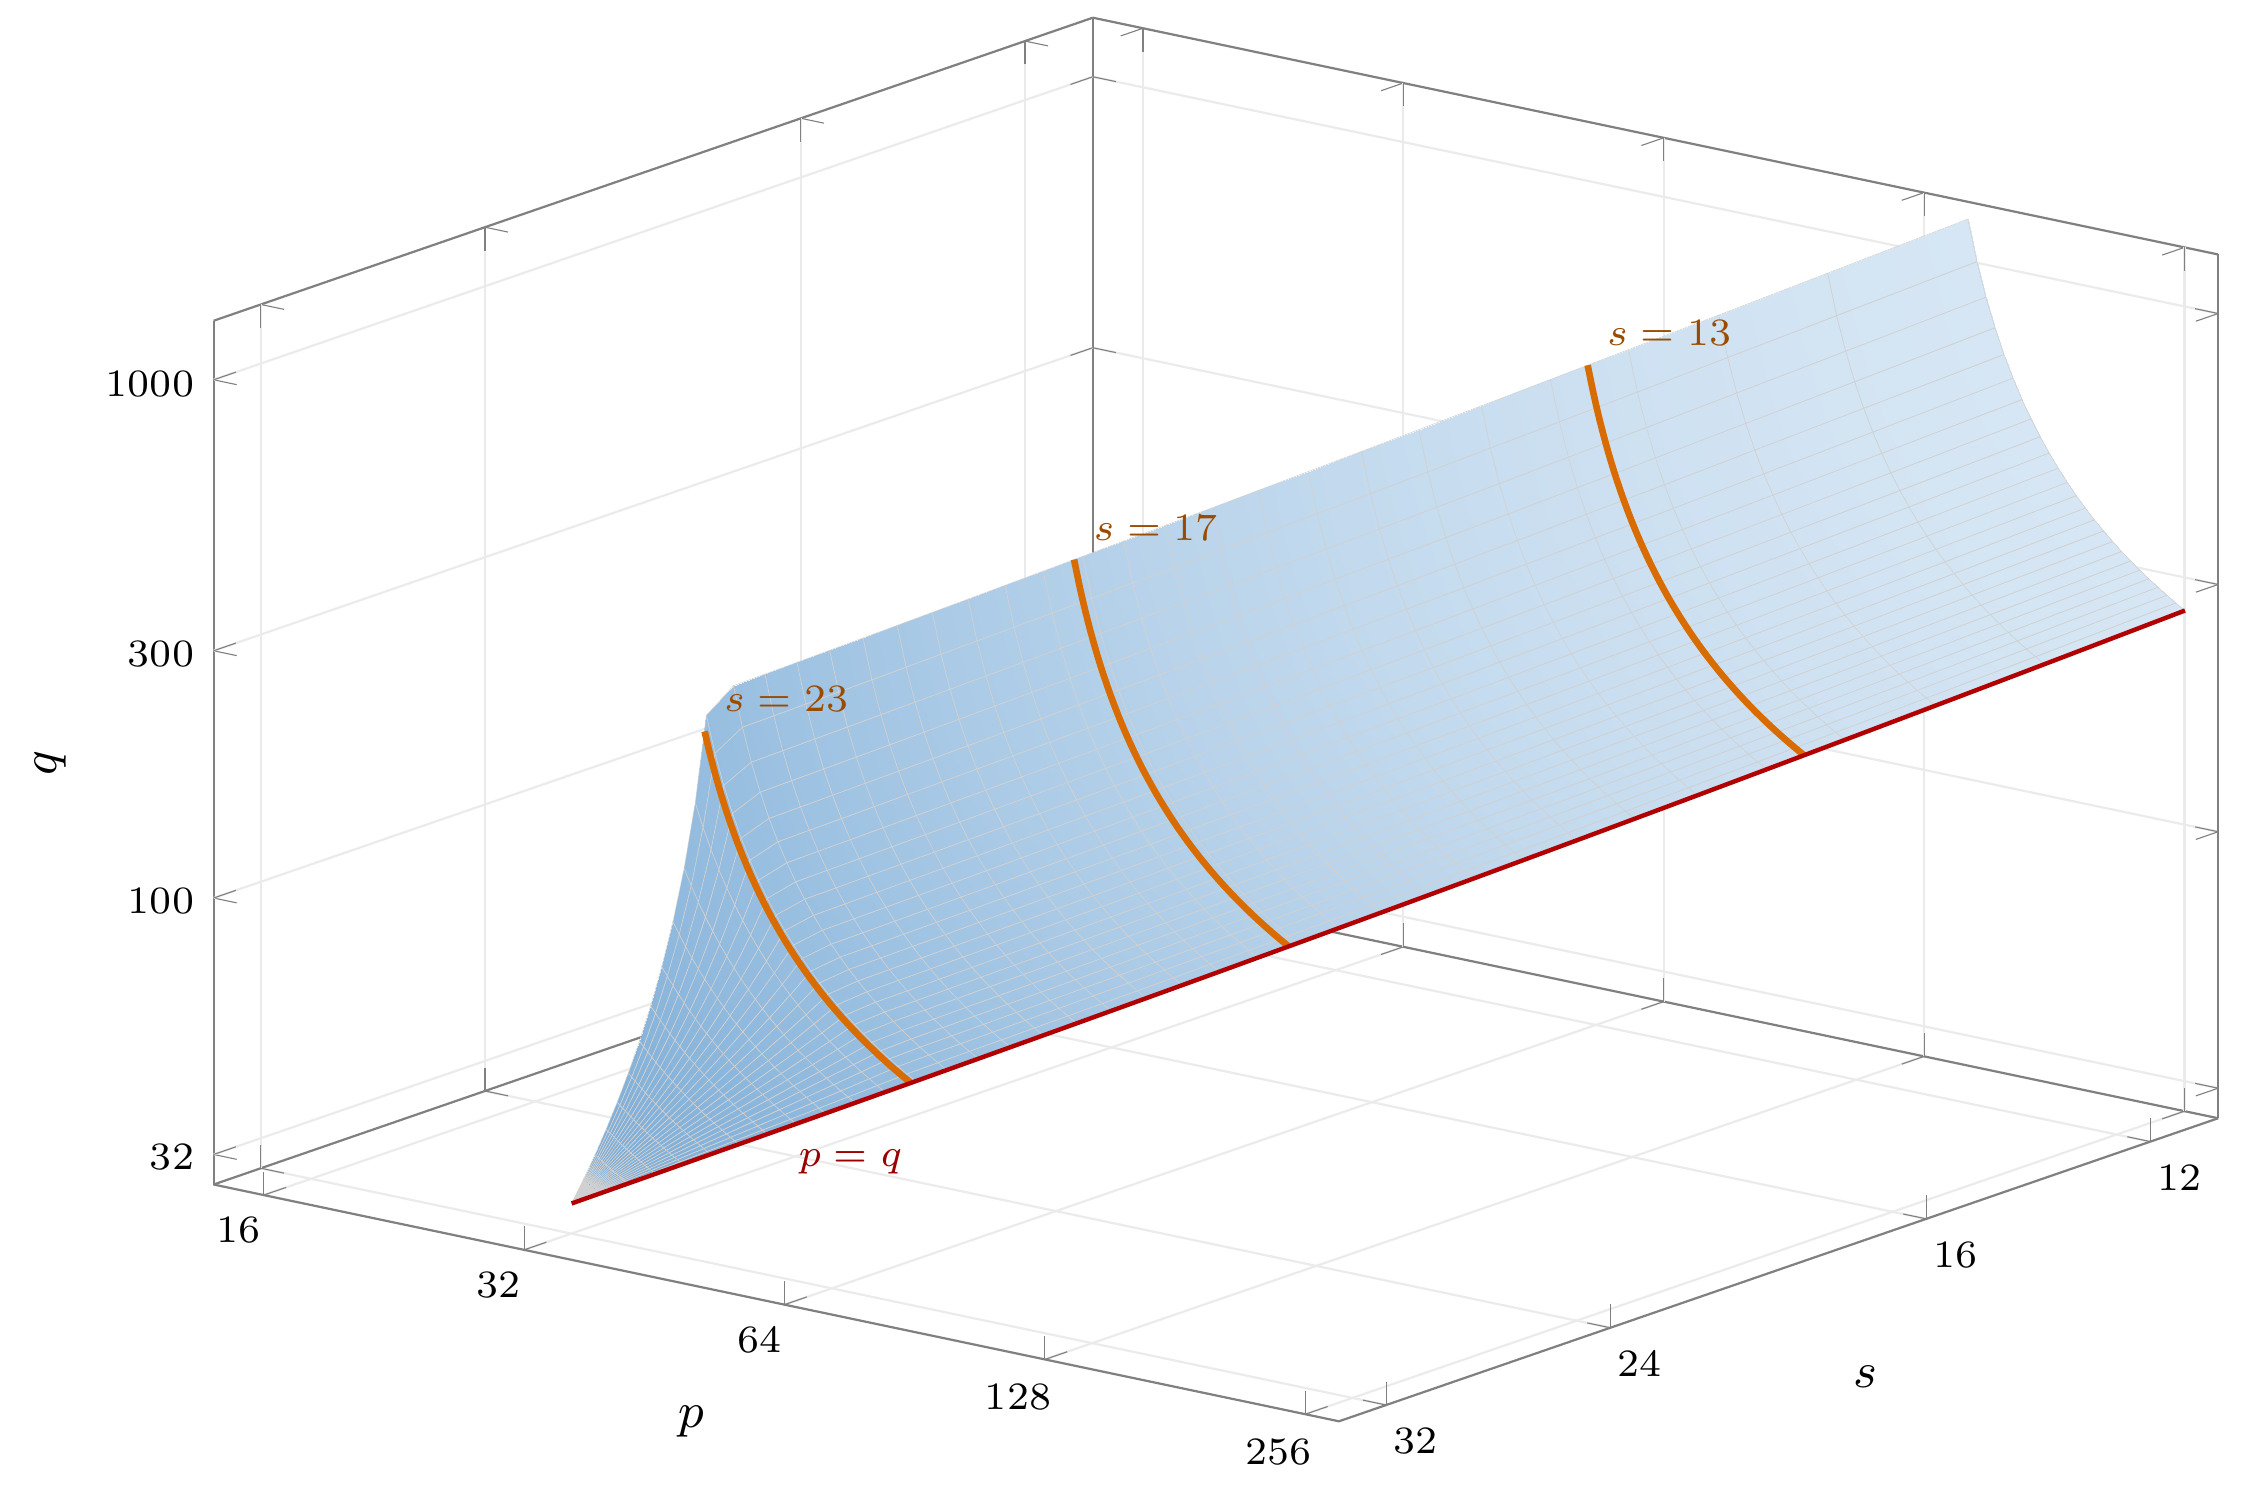
\includegraphics[width=0.86\textwidth]{figures/fig_surface.png}
\caption{The surface $\frac{s}{s-1}\cdot\frac{p}{p-1}\cdot\frac{q}{q-1}=T$
with $s<p<q$, for $T=1.1$ on logarithmic axes. Each slice with fixed
$s$, three of which are marked, falls steeply from large values of $q$
to the edge $p=q$. The slices shrink as $s$ grows, and the surface ends
at the point $s=p=q$ where $(s/(s-1))^3=T$.}
\label{fig:surface}
\end{figure}

\begin{proposition}\label{prop:class}
The integer $t=cp-2B'$ is a divisor of $N$ with
\[
  t\equiv r\pmod c,\qquad 1\le t\le\sqrt N .
\]
Moreover $\gcd(r,c)=1$ and $N\equiv r^2\pmod c$. Conversely, every
divisor $t$ of $N$ with these properties gives integers
$p=(t+2B')/c$ and $q=(N/t+2B')/c$ satisfying
$A'pq+\varepsilon=2B'(p-1)(q-1)$.
\end{proposition}

\begin{proof}
The congruence holds because $t\equiv-2B'\pmod c$, and $t\ge1$ because
both factors are positive, and $t\le\sqrt N$ because $p<q$ makes
$t$ the smaller of the two factors. Since $c=2B'-A'$ we have
$\gcd(2B',c)=\gcd(2B',A')$, which is $1$ because $A'$ is odd and, by
the congruence prune, no prime factor of $A'$ divides $B'$; hence
$\gcd(r,c)=1$. Further $N\equiv2A'B'\equiv(2B')^2\equiv r^2\pmod c$,
using $A'\equiv2B'$. Conversely, let $t$ be such a divisor. Then
$N/t\equiv r^2r^{-1}=r\pmod c$, so both $t$ and $N/t$ are congruent to
$-2B'$ and $p$ and $q$ are integers. Expanding $(cp-2B')(cq-2B')=N$ and
using $4B'^2-2A'B'=2B'c$ gives
$c\bigl(cpq-2B'(p+q)+2B'-\varepsilon\bigr)=0$, which, as $c\ge1$ and
$c=2B'-A'$, is the equation $A'pq+\varepsilon=2B'(p-1)(q-1)$.
\end{proof}

So the two-prime problem at depth $k-2$ becomes the following question:
given $N$, a modulus $c$ and a class $r$ prime to $c$, list the
divisors of $N$ up to $\sqrt N$ that are congruent to $r$ modulo $c$.
Lenstra \cite{Len84} proved that there are at most $11$ such divisors
when $c>N^{1/3}$,\footnote{In the form used here: if $0\le r<c<N$, $\gcd(r,c)=1$ and
$c>N^{1/3}$, then at most $11$ positive divisors of $N$ are congruent
to $r$ modulo $c$. The bound counts all divisors in the class, not only
those up to $\sqrt N$.} and gave a polynomial-time algorithm to find them;
Coppersmith, Howgrave-Graham and Nagaraj \cite{CHN08} extended the
algorithmic side down to $c>N^{1/4+\delta}$. We use a more elementary method suited to our range, and in
Section~\ref{sec:sum} a still simpler one based on the fact that $t$
and $N/t$ lie in the same class.

\subsection{Lattice points near a hyperbola}\label{sec:lattice}
Let $r'$ be the residue of $Nr^{-1}$ modulo $c$, so that $r'=r$ in the
situation of Proposition~\ref{prop:class}, and put
\[
  w=\frac{N-rr'}{c},\qquad \alpha\equiv wr^{-1},\qquad
  \beta\equiv r'r^{-1}\pmod c .
\]
A divisor $t\equiv r$ is written $t=r+cu$ with $u\ge0$, and then
$N/t=r'+cv$ for an integer $v$. Expanding
$(r+cu)(r'+cv)=N$ gives
\begin{equation}\label{eq:uv}
  c\,uv+r'u+rv=w ,
\end{equation}
so the pairs $(u,v)$ are the lattice points on a hyperbola. Reducing
\eqref{eq:uv} modulo $c$ shows that each of them lies in the coset
\begin{equation}\label{eq:coset}
  v\equiv\alpha-\beta u\pmod c .
\end{equation}
The coset has one point in every $c$ consecutive values of $v$ above a
given $u$, so by itself it excludes little; combined with the shape of
the hyperbola it leaves only a few points to test.

\begin{lemma}\label{lem:box}
Let $0\le u_0\le u_1$ and put
\[
  v^+=\Bigl\lfloor\frac{\lfloor N/(r+cu_0)\rfloor-r'}{c}\Bigr\rfloor,\qquad
  v^-=\Bigl\lceil\frac{\lceil N/(r+cu_1)\rceil-r'}{c}\Bigr\rceil .
\]
If $t=r+cu$ divides $N$ and $u_0\le u\le u_1$, then $N/t=r'+cv$ with
$v^-\le v\le v^+$ and $v$ satisfying \eqref{eq:coset}. Consequently,
with $H=v^+-v^-+1$, the integer $u$ lies in the set
\begin{equation}\label{eq:window}
  \bigl\{\,u\in[u_0,u_1]:\ (\alpha-\beta u-v^-)\bmod c\ <H\,\bigr\},
\end{equation}
and there is no such $t$ at all if $H\le0$.
\end{lemma}

\begin{proof}
Since $t\equiv r\pmod c$ and $\gcd(r,c)=1$, we have
$N/t\equiv Nr^{-1}\equiv r'\pmod c$, so $v=(N/t-r')/c$ is an integer.
The cofactor $N/t$ is an integer between $N/(r+cu_1)$ and
$N/(r+cu_0)$, hence between the ceiling of the first and the floor of
the second, and this gives $v^-\le v\le v^+$; in particular $H\ge1$.
The congruence \eqref{eq:coset} was shown above. Put
$x=(\alpha-\beta u-v^-)\bmod c$, so that $0\le x<c$ and
$v-v^-\equiv x\pmod c$. As $v-v^-\ge0$, it is at least the least
non-negative member $x$ of its class, and so $x\le v-v^-\le H-1$.
\end{proof}

If $H\ge c$ the set \eqref{eq:window} is the whole of $[u_0,u_1]$,
and every $u$ in the box is tested. If $H<c$ it consists of the $u$
for which an arithmetic progression modulo $c$ falls into a window of
length $H$, and its elements can be listed in increasing order without
looking at the others, at a cost of $O(\log c)$ arithmetic operations
each, by the following elementary recursion.

\begin{lemma}\label{lem:firsthit}
Let $0\le a<g$ and $0<L\le R<g$. The least $y\ge0$ with
$L\le ay\bmod g\le R$ is found as follows. If $a=0$ there is no such
$y$. If $a\ge1$ and $a\lceil L/a\rceil\le R$, it is $\lceil L/a\rceil$.
Otherwise it is $\lceil(L+gz)/a\rceil$, where $z$ is the least integer
$\ge0$ with
\[
  (-R)\bmod a\ \le\ (g\bmod a)\,z\bmod a\ \le\ (-L)\bmod a ,
\]
and if no such $z$ exists there is no $y$. The last problem is of the
same kind, with $(g,a,L,R)$ replaced by
$(a,\,g\bmod a,\,(-R)\bmod a,\,(-L)\bmod a)$.
\end{lemma}

\begin{proof}
If $a=0$ then $ay\bmod g=0<L$ for every $y$. In the second case
$ay\le R<g$ for $y=\lceil L/a\rceil$, so $ay\bmod g=ay\in[L,R]$, while
$0\le ay<L$ for smaller $y\ge0$. Otherwise no multiple of $a$ lies in
$[L,R]$. Since any $a$ consecutive integers contain a multiple of $a$,
this gives $R-L\le a-2$; moreover $a\nmid R$, and no multiple of $a$
lies in $[-R,-L]$, so the residues $(-R)\bmod a,\dots,(-L)\bmod a$ of
$-R,\dots,-L$ increase without wrapping around and
$0<(-R)\bmod a\le(-L)\bmod a<a$. A solution $y$ satisfies $ay=gz+x$
with $z=\lfloor ay/g\rfloor$ and $x=ay\bmod g\in[L,R]$, and $z\ge1$
because $z=0$ would make $x=ay$ a multiple of $a$ in $[L,R]$.
Conversely, for a given $z\ge0$ a solution with this $z$ exists
exactly when $[L+gz,R+gz]$ contains a multiple of $a$; that multiple
is unique, because $R-L<a$, and the solution is
$y=\lceil(L+gz)/a\rceil$. The
interval contains a multiple of $a$ exactly when $gz\equiv-x\pmod a$
for some $x\in[L,R]$, that is, when $gz\bmod a=(g\bmod a)z\bmod a$
lies in the stated range. The intervals $[L+gz,R+gz]$ are disjoint
and increase with $z$, since $R-L<g$, so the least $z$ gives the least
$y$.
\end{proof}

The recursion replaces $(g,a)$ by $(a,g\bmod a)$, as in Euclid's
algorithm, so it stops after $O(\log g)$ steps; Figure~\ref{fig:firsthit}
follows one step. It is applied with
$g=c$ and $a=-\beta\bmod c$ as follows. Starting from $u=u_0$, let
$b=(\alpha-\beta u-v^-)\bmod c$. If $b<H$, then $u$ is in
\eqref{eq:window}. Otherwise the next element of \eqref{eq:window}, if it
does not exceed $u_1$, is $u+y$, where $y$ is the least integer $\ge0$ with
$c-b\le ay\bmod c\le c-b+H-1$; this window lies inside $[1,c-1]$, so
Lemma~\ref{lem:firsthit} applies. Every $u$ found in this way is
tested by one exact division of $N$ by $r+cu$, and the search resumes
at $u+1$.

\begin{figure}[t]
\centering
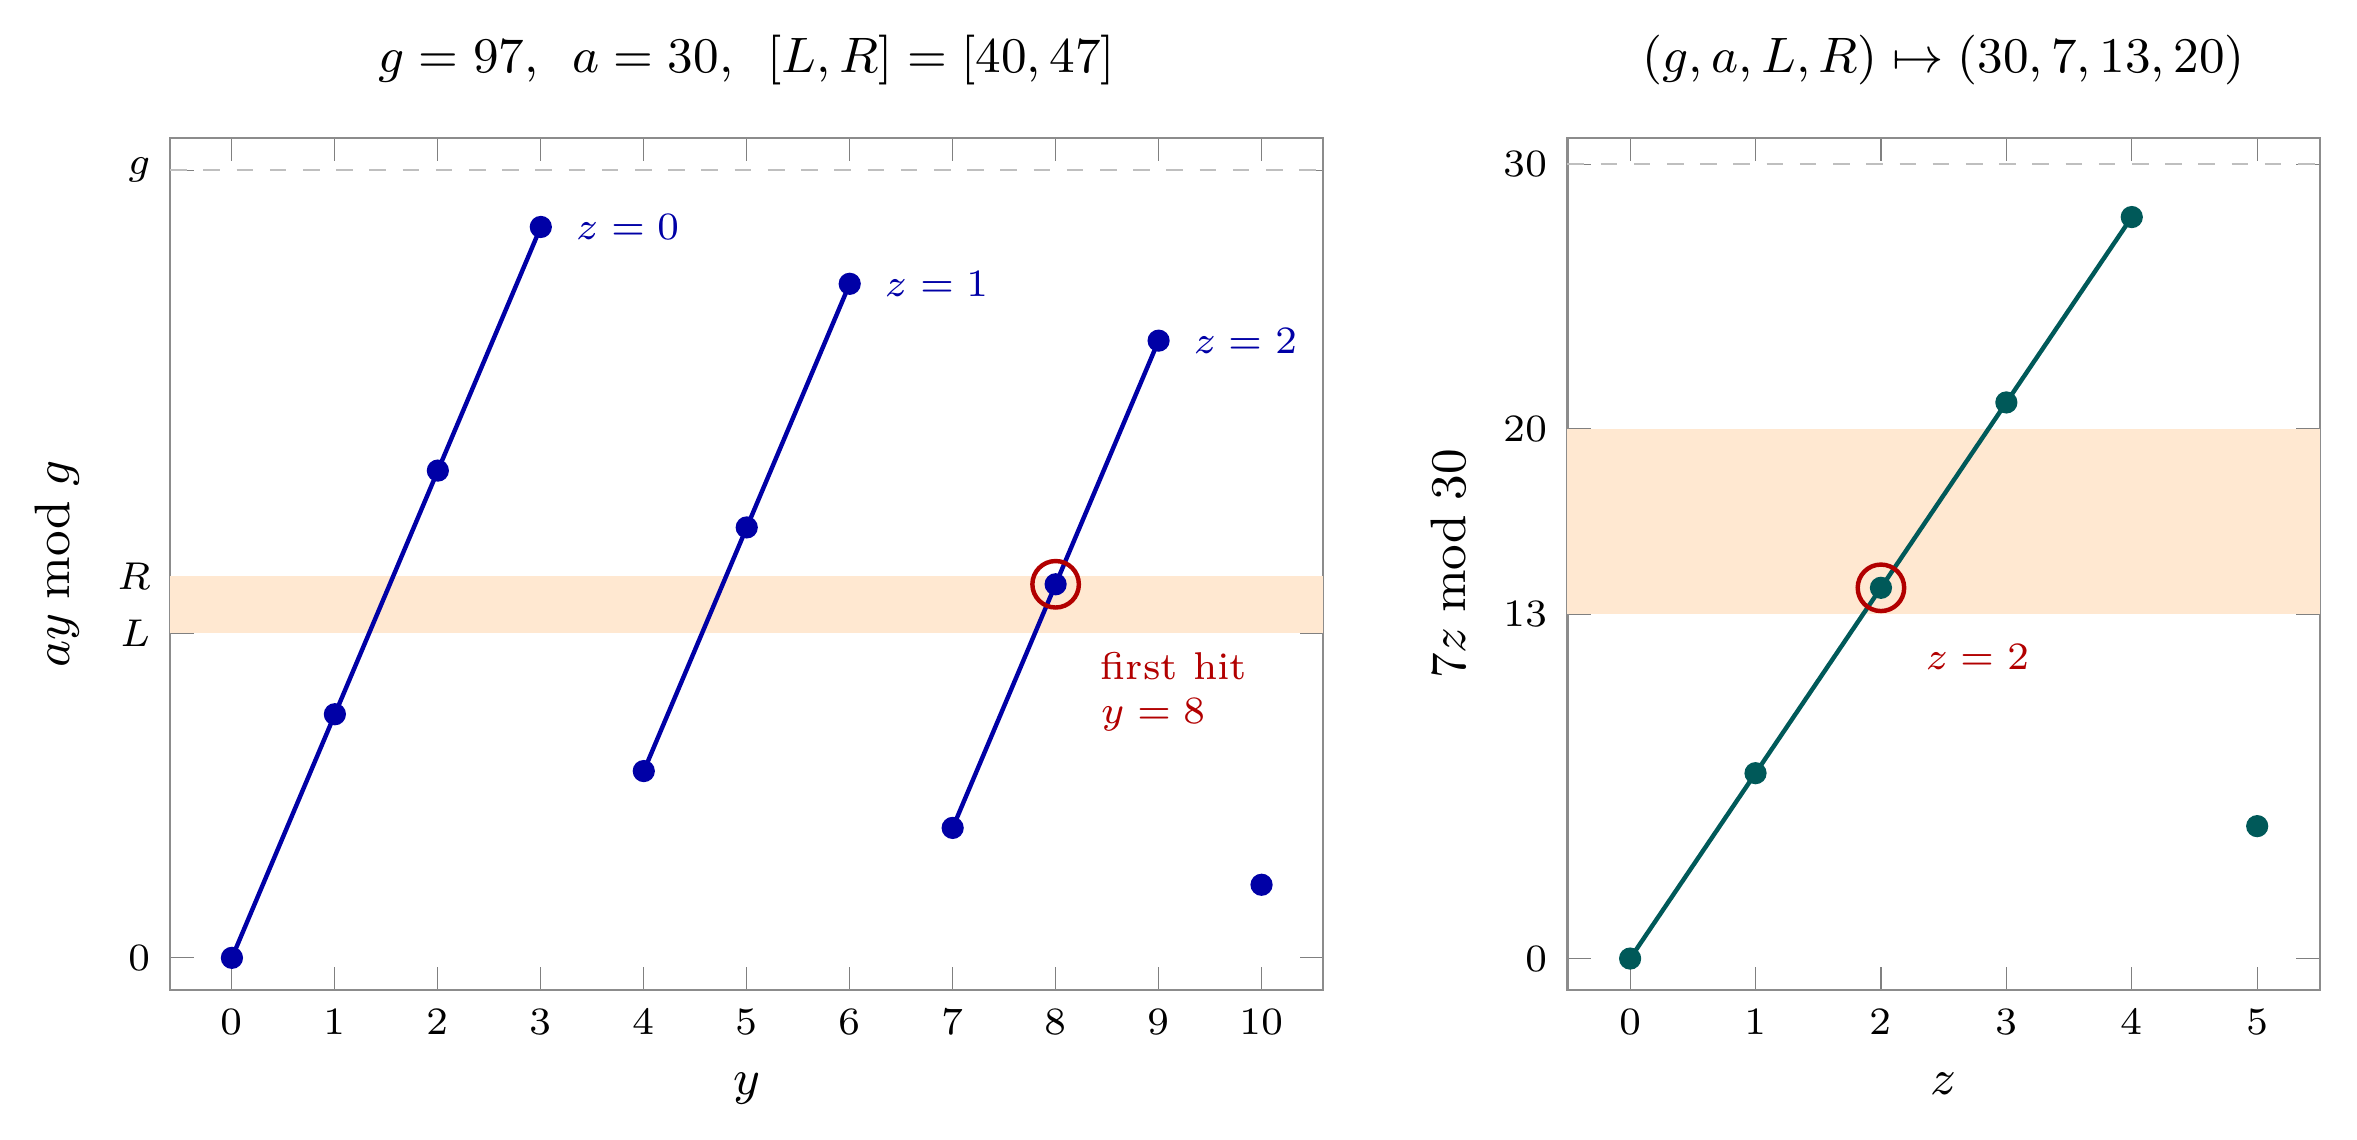
\includegraphics[width=\textwidth]{figures/fig_firsthit.png}
\caption{One step of Lemma~\ref{lem:firsthit} with $g=97$, $a=30$ and
$[L,R]=[40,47]$. Left: the residues $ay\bmod g$ rise in runs, one for
each value of $z=\lfloor ay/g\rfloor$, and the first run misses the
window because $a\lceil L/a\rceil=60>R$. Right: the reduced problem
$(30,7,13,20)$ asks for the least $z$ with $7z\bmod30$ in $[13,20]$.
It is $z=2$, and the lemma returns $y=\lceil(40+2\cdot97)/30\rceil=8$,
for which $ay\bmod g=46$.}
\label{fig:firsthit}
\end{figure}

\begin{figure}[t]
\centering
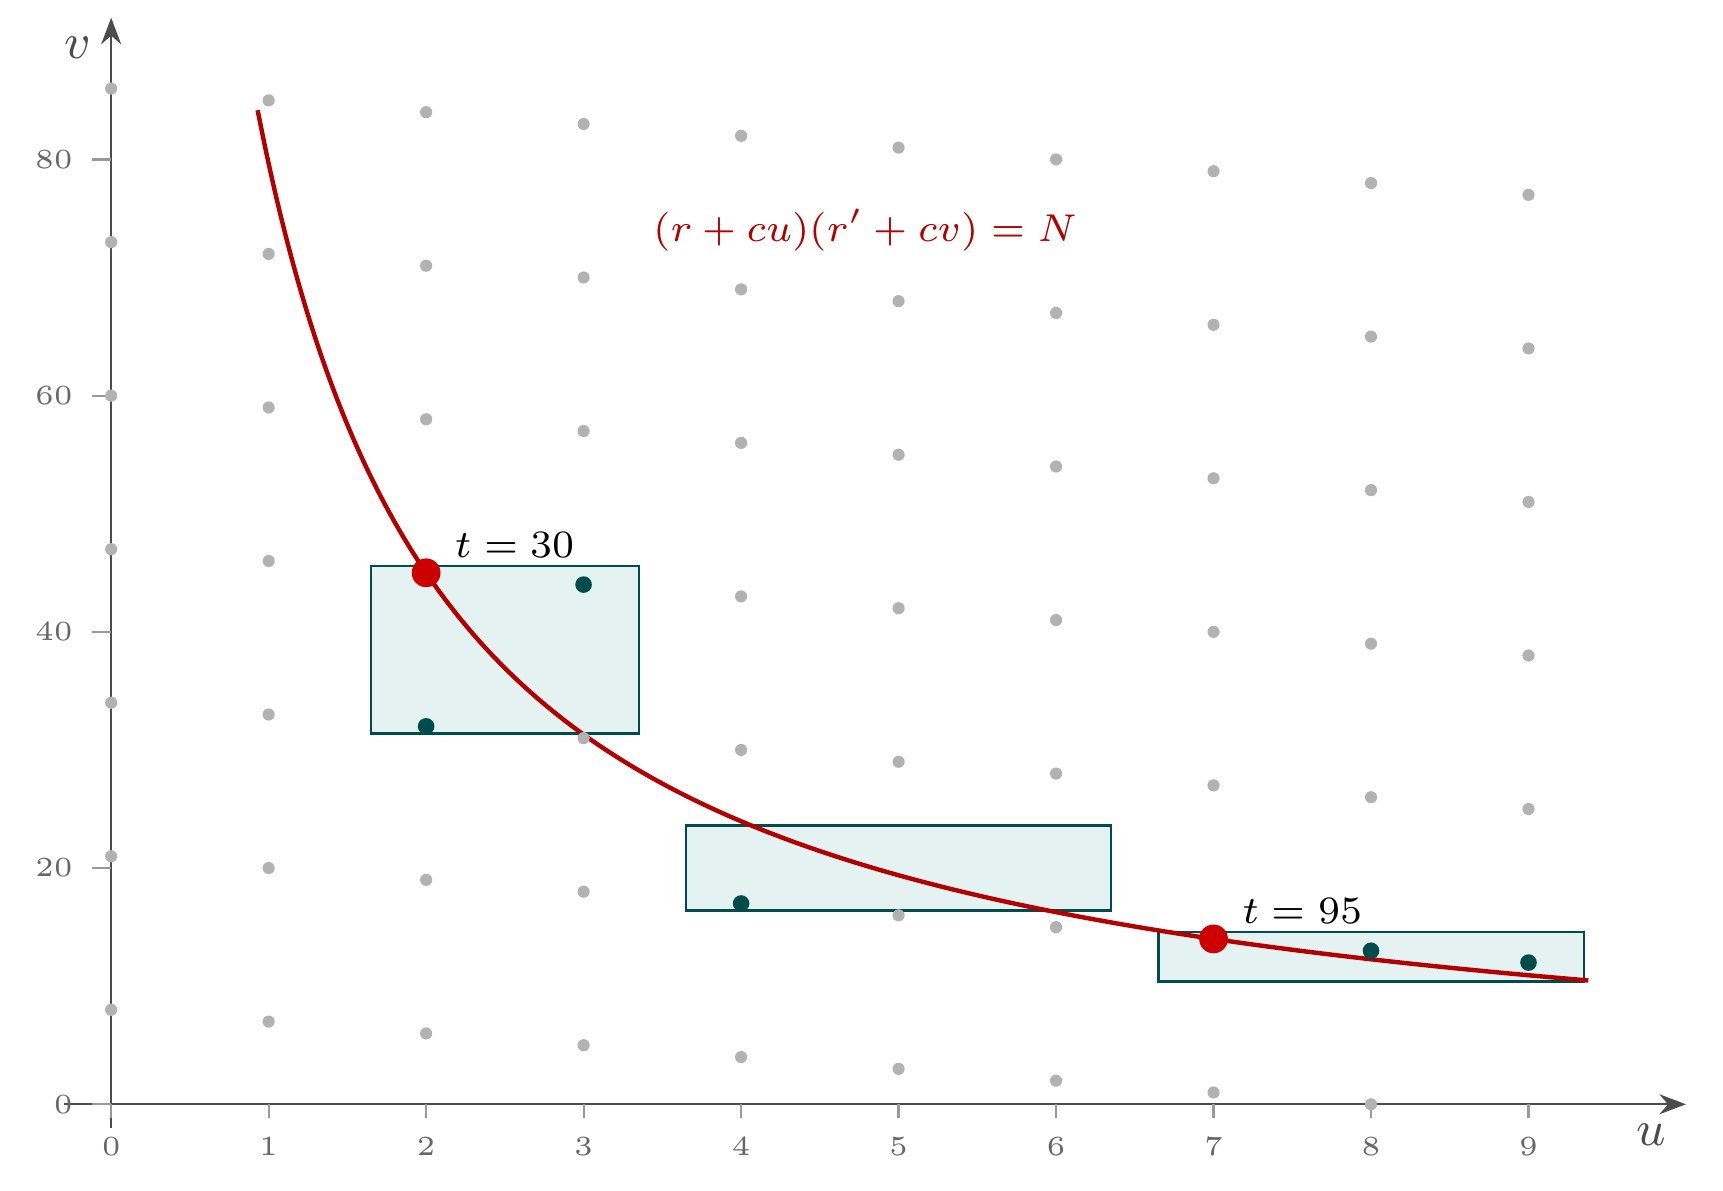
\includegraphics[width=0.69\textwidth]{figures/fig_boxes.png}
\caption{The divisors of $N=17670$ in the class $4$ modulo $13$ up to
$\sqrt N$, found as in Lemma~\ref{lem:box}. The grey points form the
coset \eqref{eq:coset}, here $v\equiv8-u\pmod{13}$; the curve is the
hyperbola \eqref{eq:uv}. The boxes cover the curve for $2\le u\le9$
(the values $u=0,1$ are tested directly), and only the points inside a
box are examined. Two of them lie on the curve and give the divisors
$t=30$ and $t=95$.}
\label{fig:boxes}
\end{figure}

\subsection{Choosing the boxes}
The range $0\le u\le U=\lfloor(\lfloor\sqrt N\rfloor-r)/c\rfloor$ is
cut into consecutive intervals $[u_0,u_1]$, each giving a box
$[u_0,u_1]\times[v^-,v^+]$ in Lemma~\ref{lem:box}
(Figure~\ref{fig:boxes}). Correctness does not depend on how this is
done; the choice only affects the running time. Since
$v\approx K/u$ with $K=N/c^2$, a box with $u_1-u_0=\lambda u_0$ has
area close to $K\lambda^2/(1+\lambda)$, and as the coset has one point
per area $c$ we choose $\lambda$ with $\lambda^2/(1+\lambda)=c^3/N$, so
that each box holds about one point of \eqref{eq:coset}. There are two
regimes. If $c^3>N$, then $\lambda$ exceeds $1.6$ and grows like
$c^3/N$, so that $O\bigl(\log N/\log(2+c^3/N)\bigr)$ boxes cover the
whole range: this is Lenstra's range, and the work is a handful of
Euclidean recursions. If $c^3<N$,
the boxes shrink to width about $u_0(c^3/N)^{1/2}$, the values of $u$
below $(N/c^3)^{1/2}$ are tested one at a time, and the number of
boxes grows like $(N/c^3)^{1/2}\log N$. When this estimate exceeds a
fixed threshold we factor $N$ completely instead and read off its
divisors in the class.

\begin{theorem}\label{thm:three}
Let $(p_1,\dots,p_{k-3})$ be a node at depth $k-3$ of the search of
Section~\ref{sec:search}. Every $n=p_1\cdots p_k$ with
$n+\varepsilon=2\varphi(n)$ extending this node is found by running
$s=p_{k-2}$ over the admissible primes of its interval and, for each
$s$, listing the divisors of Proposition~\ref{prop:class} by
Lemmas~\ref{lem:box} and~\ref{lem:firsthit} or by a complete
factorisation of $N$.
\end{theorem}

\begin{proof}
The prime $p_{k-2}$ lies in the interval and passes the prune, as in
the proof of Theorem~\ref{thm:complete}. For $s=p_{k-2}$,
Proposition~\ref{prop:class} shows that $t=cp_{k-1}-2B'$ is one of the
divisors listed: Lemma~\ref{lem:box} shows that $u=(t-r)/c$ lies in
the set \eqref{eq:window} of the box that contains it, and
Lemma~\ref{lem:firsthit} lists every element of that set, or, if
$N$ is factored, $t$ is read off from its factorisation. The converse part of
Proposition~\ref{prop:class} then recovers $p_{k-1}$ and $p_k$.
\end{proof}

Every divisor that is found yields integers $p\le q$ with
$A_{k-3}spq+\varepsilon=2B_{k-3}(s-1)(p-1)(q-1)$, by the converse part
of Proposition~\ref{prop:class}, and $n=p_1\cdots p_{k-3}\,s\,pq$ is a
solution exactly when $s<p<q$ and $p$ and $q$ are prime. As before, the correctness of a
negative answer depends on no primality proof except in the factoring
route, where every prime factor of $N$ is proved prime
(Appendix~\ref{app:primality}).

\subsection{The sum of the two factors}\label{sec:sum}
The classes of Proposition~\ref{prop:class} are special: $t$ and $N/t$
lie in the same class modulo $c$, because $N\equiv r^2$. This allows a
third treatment which uses neither boxes nor factoring. Write $t=r+cu$
and $N/t=r+cv$ with $0\le u\le v$. Since $r'=r$, the integer $w$ of Section~\ref{sec:lattice} is $w=(N-r^2)/c$, and \eqref{eq:uv} becomes
\begin{equation}\label{eq:sum}
  c\,uv+r\,(u+v)=w ,
\end{equation}
so the sum $S=u+v$ lies in the single class $S\equiv wr^{-1}\pmod c$,
and $u$ and $v$ are the roots of $X^2-SX+(w-rS)/c$. Conversely, if
$S\equiv wr^{-1}\pmod c$, then $(w-rS)/c$ is an integer, and if
$S^2-4(w-rS)/c=e^2$ with an integer $e\ge0$ of the parity of $S$, then
$u=(S-e)/2$ and $v=(S+e)/2$ are integers satisfying \eqref{eq:sum}, so
that $(r+cu)(r+cv)=N$. Fix $u_d\ge1$ and put $t_d=r+cu_d$; if
$t_d>\sqrt N$ there is no divisor with $u\ge u_d$ to look for. Since
$x+N/x$ decreases on $(0,\sqrt N\,]$, every divisor $t\le\sqrt N$ with
$u\ge u_d$ has $2r+cS=t+N/t\le t_d+N/t_d$, while $t+N/t\ge2\sqrt N$.
So $S$ runs over at most $N/(c^3u_d)+1$ values of one residue class,
and each value needs a single test whether $S^2-4(w-rS)/c$ is a
perfect square. Every divisor with $u\ge u_d$ is found in this way,
and by the converse every square found gives a factorisation
$N=(r+cu)(r+cv)$. The divisors with $u<u_d$ are found by trial division. With $u_d$ close to $(N/c^3)^{1/2}$ the work
is about $2(N/c^3)^{1/2}+2$ operations. This is comparable with the
number of boxes above, but unlike the work in the boxes it does not
depend on where the divisors lie.

The same argument bounds the number of divisors.

\begin{proposition}\label{prop:fourdiv}
In the situation of Proposition~\ref{prop:class}, suppose that
$c^3\ge N+2c^2$. Then at most one divisor $t\le\sqrt N$ of $N$ with
$t\equiv r\pmod c$ is different from $r$, and $N$ has at most four
positive divisors congruent to $r$ modulo $c$.
\end{proposition}

\begin{proof}
By Proposition~\ref{prop:class}, every divisor $t$ of $N$ in the
class has $N/t\equiv r^2r^{-1}=r\pmod c$. Let $t_1<t_2\le\sqrt N$ be
divisors of $N$ in the class, both different from $r$. The hypothesis
gives $c^3>2c^2$, so $c>2$ and $0<r<c$. Hence $t_i=r+cu_i$ with
$u_i\ge1$, and $N/t_i=r+cv_i$ with $v_i\ge u_i$. By \eqref{eq:sum} the sums
$u_i+v_i$ lie in one class modulo $c$, so the numbers
$t_i+N/t_i=2r+c(u_i+v_i)$ differ by a multiple of $c^2$. The difference
is positive, because $x+N/x$ decreases on $(0,\sqrt N\,]$, and both
numbers lie between $2\sqrt N$ and $r+c+N/(r+c)<2c+N/c$. Hence
$c^2<2c+N/c-2\sqrt N<2c+N/c$, that is, $c^3<N+2c^2$, contrary to the
hypothesis. Finally, every divisor of $N$ above $\sqrt N$ in the class
is $N/t$ for a divisor $t<\sqrt N$ in the class, and so there are at
most four divisors in the class: $r$, $N/r$, $t$ and $N/t$.
\end{proof}

For classes of this special kind, and at the price of the term $2c^2$,
Proposition~\ref{prop:fourdiv} sharpens Lenstra's bound of $11$ to
four.

We ran this route, too, over every pair of a node at depth $k-3$ and
an admissible $s$. It takes its primes $s$ from a sieve of its own and
uses no factorisation, so its negative answers depend on no primality
test at all.

%%==================================================================
\section{Lehmer's equation: proof of Theorem~\ref{thm:first}}\label{sec:first}
%%==================================================================

The last two assertions of Theorem~\ref{thm:first} were proved in
Section~\ref{sec:indep}. For the first, let $n$ be composite with
$\varphi(n)\mid n-1$ and suppose $\omega(n)\le15$. By
Lemma~\ref{lem:three}, $3\nmid n$; by
Lemma~\ref{lem:basic}(i), $n=p_1\cdots p_k$ with $5\le p_1<\dots<p_k$
and $k\le15$; and by Lemma~\ref{lem:Mtwo}, $n-1=2\varphi(n)$. If
$k\le6$ then $\prod p_i/(p_i-1)\le\prod_{i\le6}r_i/(r_i-1)=1.9490\ldots$,
which contradicts \eqref{eq:excess}. It therefore suffices to run the
search with $\varepsilon=-1$ and $p_{\min}=5$ for $7\le k\le15$, and to
find nothing. For $k\le14$ we use the search of
Section~\ref{sec:search}, and for $k=15$ the method of
Section~\ref{sec:three}.

\subsection{Up to fourteen primes}

Table~\ref{tab:first} records the outcome. The column \emph{terminal}
counts the nodes at depth $k-2$ whose interval for $p_{k-1}$ is
non-empty, and the last column gives the largest width $U_{k-2}-L_{k-2}$
of such an interval. No solution was found for any $k\le14$, so by
Theorem~\ref{thm:complete} there is none. The case $k\le13$ recovers
the theorem of Cohen and Hagis, and the case $k=14$ is the bound
$\omega(n)\ge15$ announced by Renze and by Pinch.

\begin{table}[ht]
\centering
\caption{The search for $n-1=2\varphi(n)$ with $5\le p_1$. Both
implementations visit the same number of nodes for every $k$.}
\label{tab:first}
\smallskip
\begin{tabular}{@{}rrrr@{}}
\toprule
$k$ & nodes & terminal & largest width for $p_{k-1}$ \\
\midrule
 7 &      8 &      0 &            -- \\
 8 &     18 &      1 &             2 \\
 9 &     29 &      1 &             3 \\
10 &     42 &      1 &             2 \\
11 &     73 &      7 &            49 \\
12 &    187 &     61 &           298 \\
13 & 1\,092 &    725 &       25\,854 \\
14 & 31\,962 & 29\,549 & 54\,962\,375 \\
\bottomrule
\end{tabular}
\end{table}

For $k=14$ the numbers of nodes at depths $0,1,\dots,12$ are
\[
  1,\ 6,\ 16,\ 27,\ 29,\ 23,\ 22,\ 33,\ 58,\ 127,\ 335,\ 1654,\ 29631,
\]
as in the row $k=14$ of Figure~\ref{fig:profile}, and $82$ of the $29631$ nodes at depth $12$ have an empty interval for
$p_{13}$. The largest prime occurring at depth $12$ is $77563$. Most of
the work lies in a few terminal nodes. Exactly
fifteen have an interval for $p_{13}$ of width more than three million;
they are listed in Table~\ref{tab:hard}. Each of these intervals was
enumerated in full, and independently the integer $D=2AB-C$ was
factored completely for each of the fifteen; the factorisations are
part of the archived data.

\begin{table}[ht]
\centering
\caption{The fifteen terminal nodes of the case $k=14$ with an interval
for $p_{13}$ of width more than $3\cdot10^6$, with the number of digits
of $D=2AB-C$.}
\label{tab:hard}
\smallskip
\small
\begin{tabular}{@{}lrr@{}}
\toprule
$p_1,\dots,p_{12}$ & width & digits of $D$ \\
\midrule
5, 7, 13, 17, 19, 23, 37, 59, 67, 89, 173, 25867  & 54\,962\,375 & 41 \\
5, 7, 13, 17, 19, 23, 37, 59, 67, 89, 173, 25889  & 19\,589\,597 & 41 \\
5, 7, 13, 17, 19, 23, 37, 59, 67, 73, 317, 5483   & 14\,242\,697 & 40 \\
5, 7, 13, 17, 19, 23, 37, 59, 67, 89, 173, 25903  & 13\,903\,362 & 41 \\
5, 7, 13, 17, 19, 23, 37, 59, 67, 89, 173, 25913  & 11\,517\,582 & 41 \\
5, 7, 13, 17, 19, 23, 37, 59, 67, 89, 173, 25919  & 10\,443\,048 & 41 \\
5, 7, 13, 17, 19, 23, 37, 59, 67, 89, 173, 25933  &  8\,577\,304 & 41 \\
5, 7, 13, 17, 19, 23, 37, 59, 67, 89, 173, 25939  &  7\,967\,703 & 41 \\
5, 7, 13, 17, 19, 23, 37, 59, 83, 97, 107, 3343   &  6\,121\,542 & 39 \\
5, 7, 13, 17, 19, 23, 37, 59, 67, 97, 199, 577    &  6\,086\,511 & 38 \\
5, 7, 13, 17, 19, 23, 37, 59, 67, 89, 173, 25969  &  5\,880\,810 & 41 \\
5, 7, 13, 17, 19, 23, 37, 59, 67, 89, 173, 26003  &  4\,537\,275 & 41 \\
5, 7, 13, 17, 19, 23, 37, 59, 67, 89, 173, 26017  &  4\,147\,802 & 41 \\
5, 7, 13, 17, 19, 23, 37, 59, 67, 89, 173, 26029  &  3\,863\,803 & 41 \\
5, 7, 13, 17, 19, 23, 37, 59, 83, 109, 173, 199   &  3\,320\,179 & 37 \\
\bottomrule
\end{tabular}
\end{table}

Eleven of the fifteen share the prefix
$5,7,13,17,19,23,37,59,67,89,173$, whose product
$\prod p/(p-1)$ is already within $8\cdot10^{-5}$ of $2$; the twelfth
prime then closes most of the remaining gap. For the node ending in
$25867$ one has $T-1=C/A=1.8\cdot10^{-8}$, and for the node ending in
$5483$ one has $T-1=7.0\cdot10^{-8}$. These near misses are the
reason the width of the last interval grows so quickly with $k$: by
Proposition~\ref{prop:bounds} with $m=2$ the interval for $p_{k-1}$
runs from about $A/C$ to about $2A/C$, and a small $C$ means a long
interval. For the node ending in $25867$ this gives exactly the
interval $[54962376,\,109924751]$. Among
the fifteen integers $D$ one, for the node ending in $25913$, is itself
a prime of $41$ digits\footnote{For this node \eqref{eq:hyperbola} has
only the trivial factorisations $D=1\cdot D$ and $D=D\cdot1$, and
neither gives a pair of primes in the required range. The enumeration
of the $1.15\cdot10^7$ candidates for $p_{13}$ reaches the same
conclusion without knowing that $D$ is prime.}.

\begin{figure}[t]
\centering
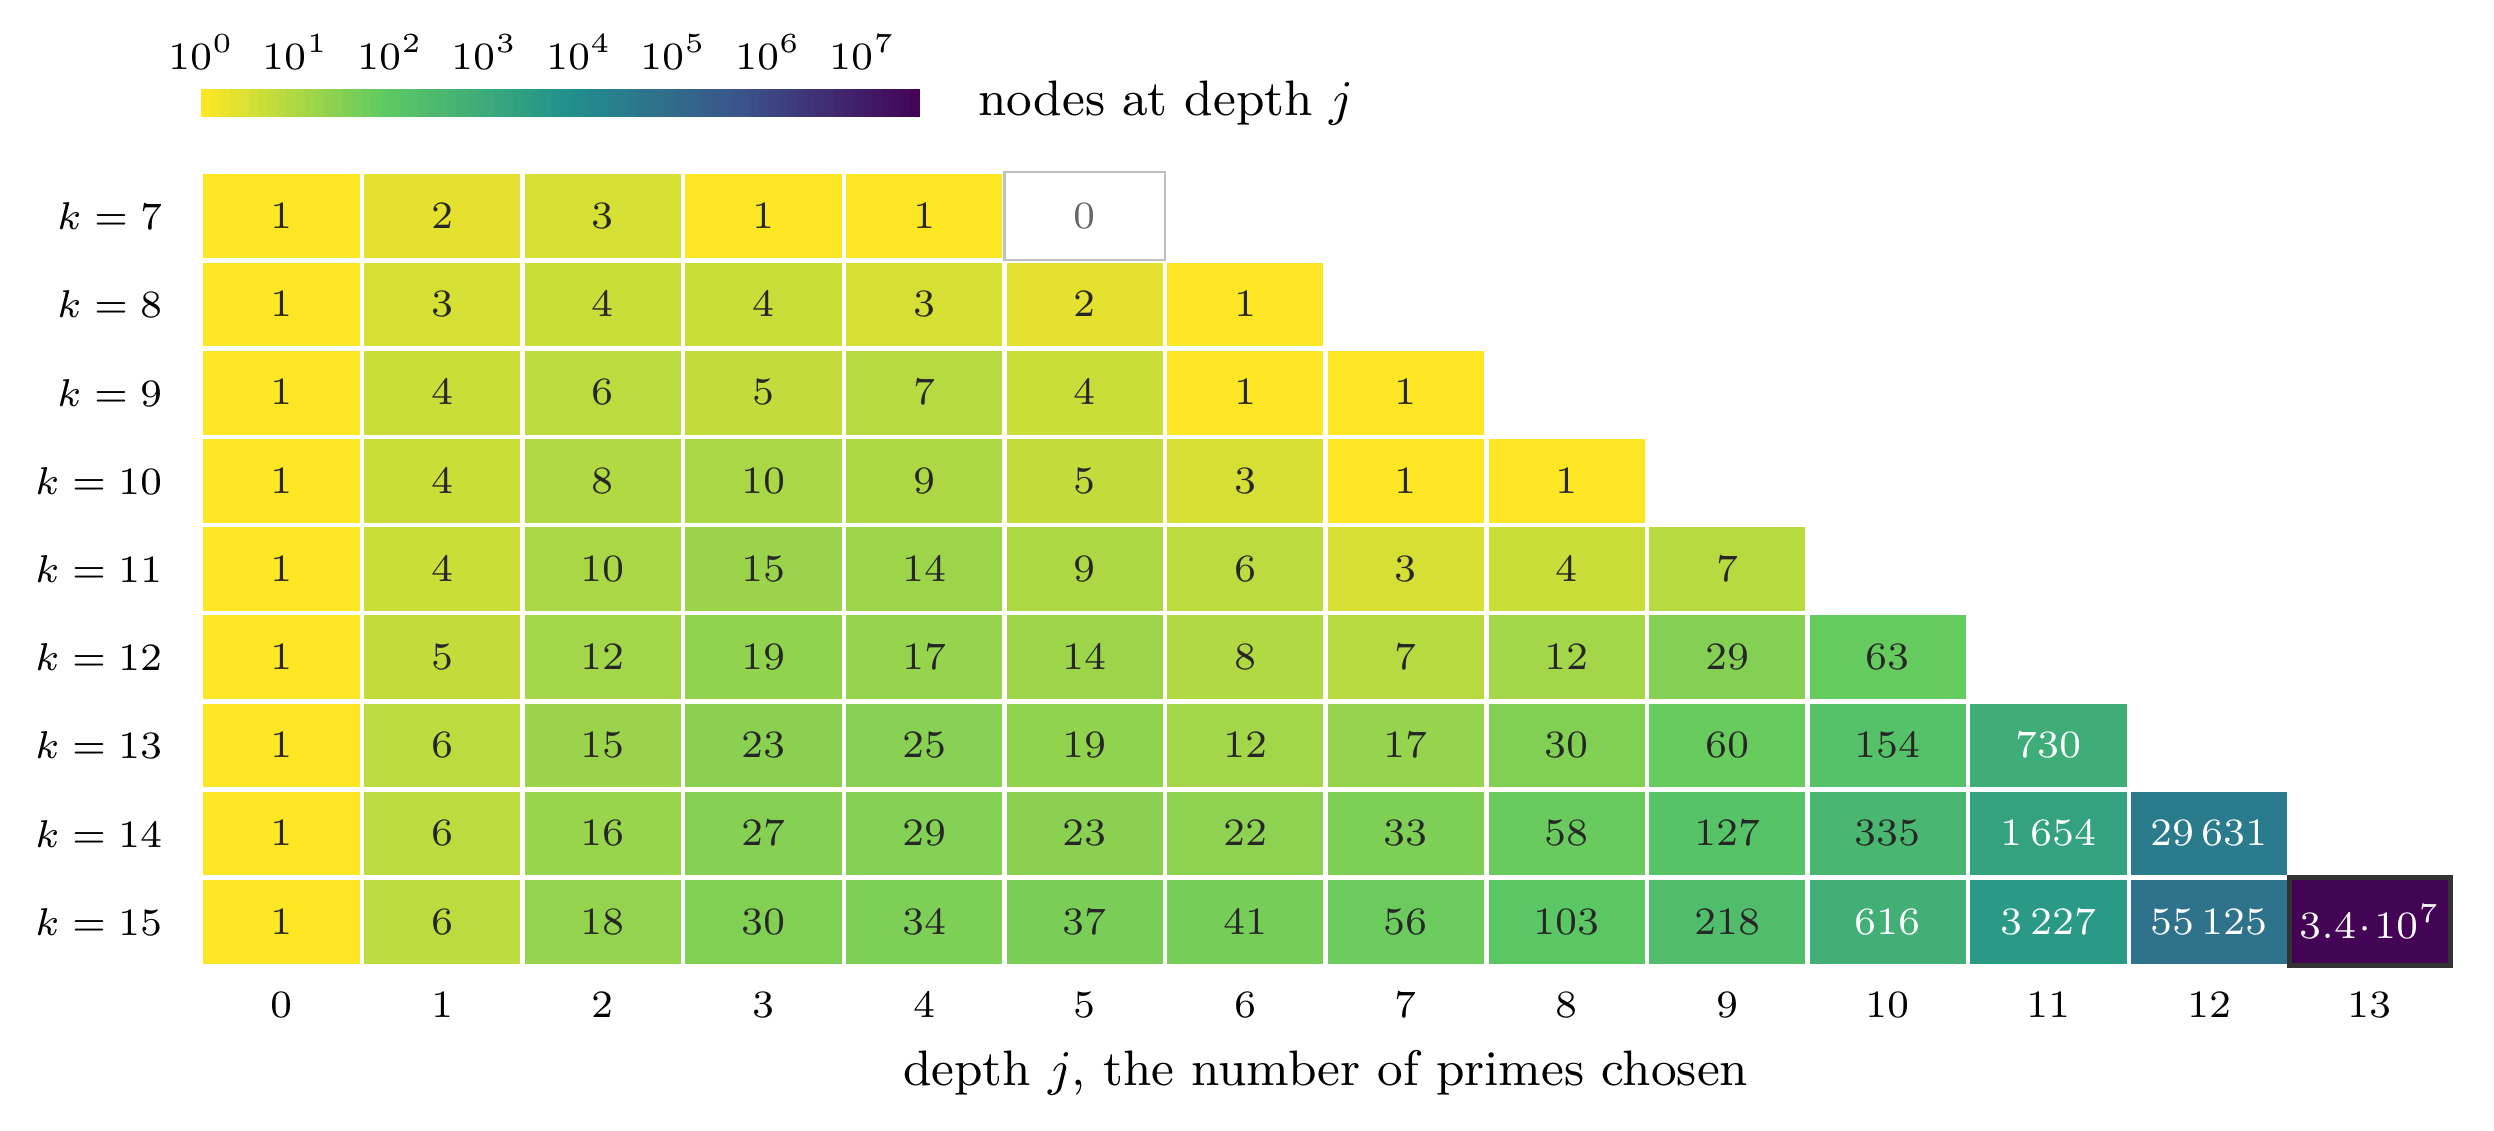
\includegraphics[width=\textwidth]{figures/fig_profile.png}
\caption{Number of nodes at each depth $j$ of the search for
$k=7,\dots,15$ primes, with the colour on a logarithmic scale. The
counts are the same for $n-1=2\varphi(n)$ and $n+1=2\varphi(n)$ with
$p_1\ge5$. The tree stays small until the last two levels. The last
cell of each row counts the nodes at depth $k-2$: for $k\le14$ these
are the nodes where $p_{k-1}$ is enumerated, and for $k=15$ (framed)
they are the $33865004$ choices of $p_{13}$, each completed by the
method of Section~\ref{sec:three}.}
\label{fig:profile}
\end{figure}

\subsection{Fifteen primes}\label{sec:fifteen}
\begin{figure}[t]
\centering
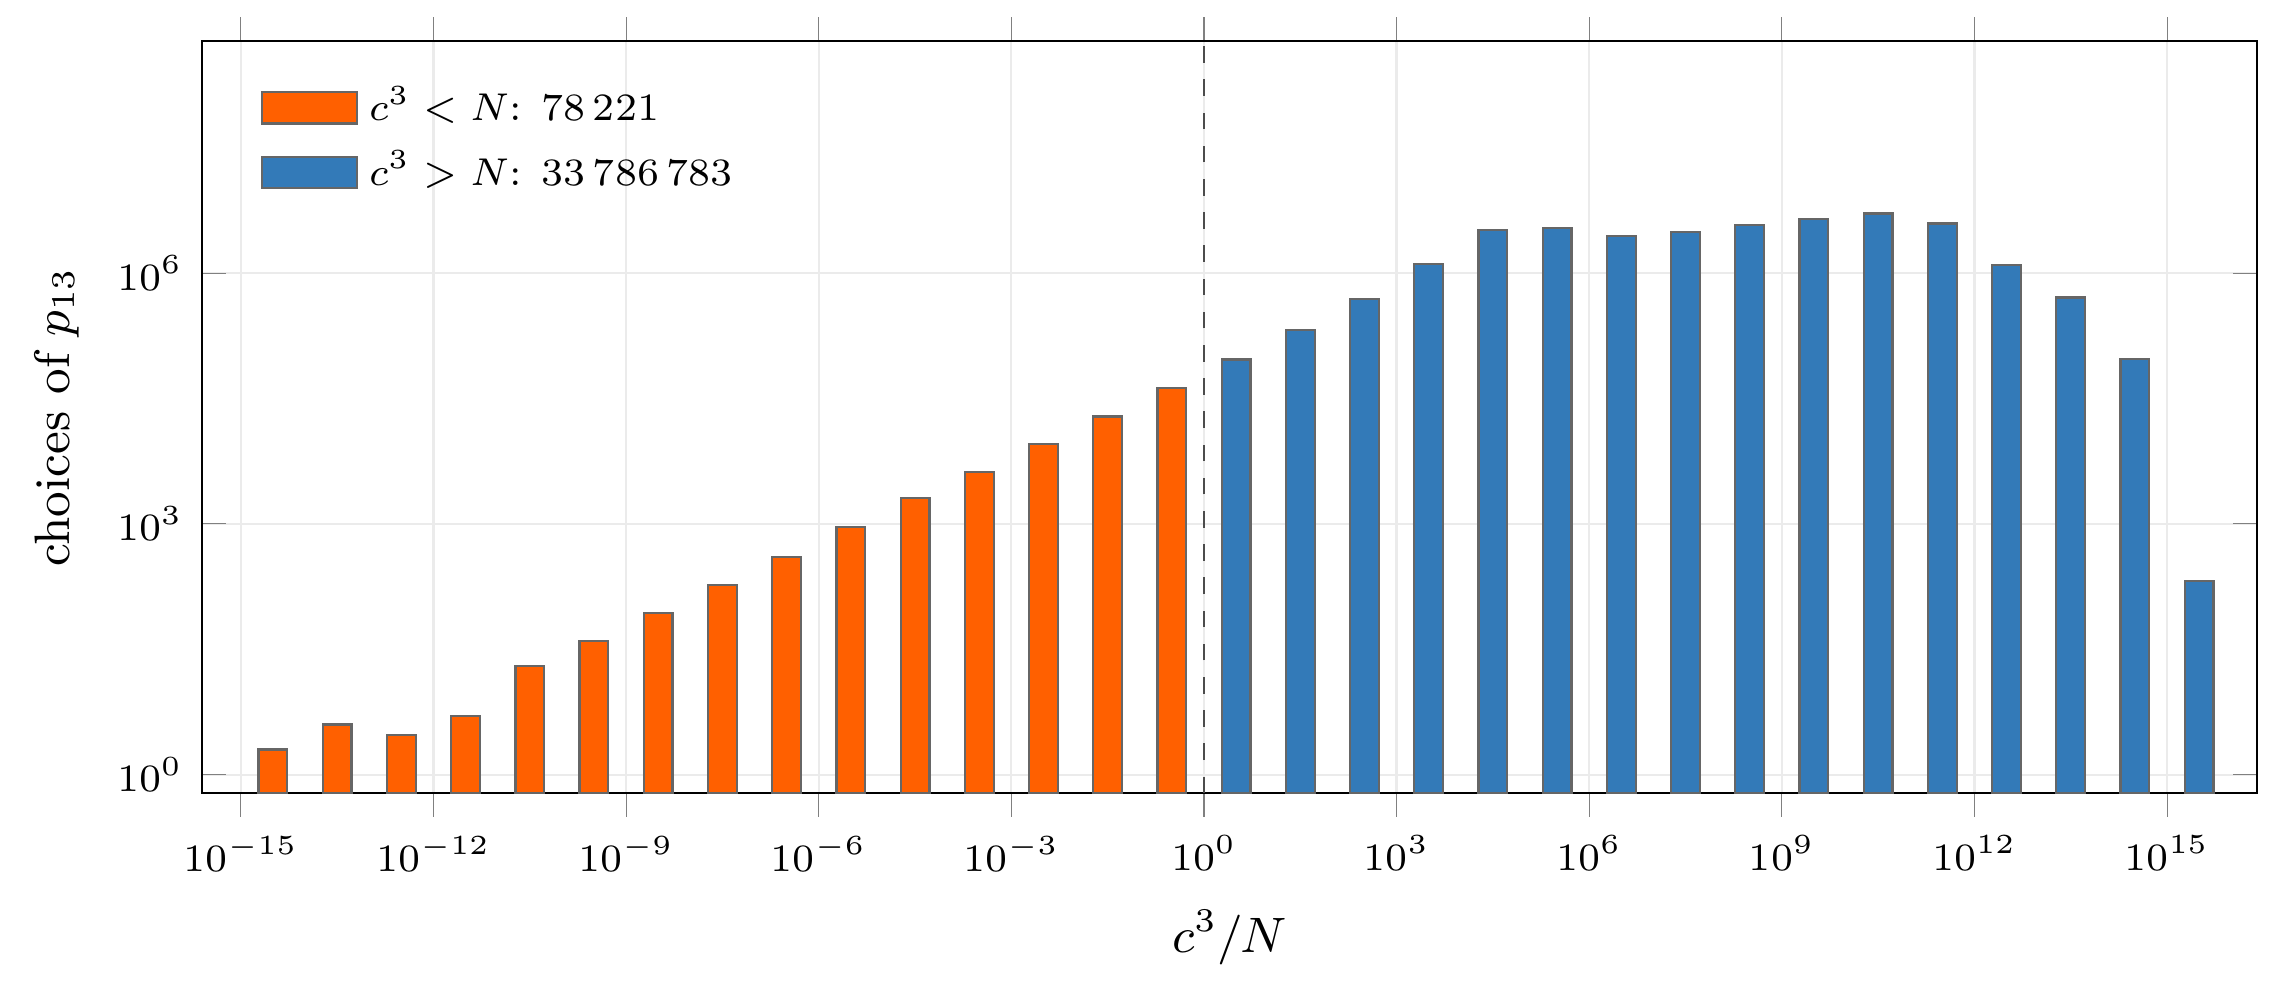
\includegraphics[width=0.92\textwidth]{figures/fig_k15.png}
\caption{The $33865004$ two-prime problems of the case $k=15$, by the
ratio $c^3/N$ on a logarithmic scale (bins of one decade). To the right
of the dashed line is Lenstra's range, where $N$ has at most $11$
divisors in the class and a few boxes find them. The left tail comes
from the lower ends of the longest intervals for $p_{13}$.}
\label{fig:k15}
\end{figure}

For $k=15$ the traversal of Section~\ref{sec:search} is stopped at
depth $12$. The numbers of nodes at depths $0,1,\dots,12$ are
\[
  1,\ 6,\ 18,\ 30,\ 34,\ 37,\ 41,\ 56,\ 103,\ 218,\ 616,\ 3227,\ 55125,
\]
and $54985$ of the nodes at depth $12$ have a non-empty interval for
$p_{13}$. Both implementations of the search (Appendix~\ref{app:two}) produce the
same $54985$ prefixes with the same intervals, and so do the bounds
for $\varepsilon=+1$. The intervals have total length
$1.005\cdot10^9$ and contain $33865004$ primes $s$ that pass the
congruence prune. For each of these pairs of a prefix and a prime
$s=p_{13}$ we solved the two-prime problem of
Proposition~\ref{prop:class}, in which $N$ has between $40$ and $58$
digits, three times: by the two implementations of the lattice method
(Section~\ref{sec:lattice} and Appendix~\ref{app:second}) and by the
route of Section~\ref{sec:sum}.

Figure~\ref{fig:k15} shows how the pairs are distributed according to
the ratio $c^3/N$, which by Section~\ref{sec:three} decides how hard
the two-prime problem is. For $33786783$ of them, all but $0.23$ per
cent, the modulus satisfies $c^3>N$, so that Lenstra's bound applies
and a few boxes suffice. The remaining $78221$ pairs come from values
of $s$ just above the lower end of long intervals, where
$c=C_{12}s-2B_{12}$ is small. The most extreme is the prefix ending in
$25867$ of Table~\ref{tab:hard}, whose first admissible $s$ gives
$c^3/N\approx2\cdot10^{-15}$. For these pairs the route of
Section~\ref{sec:sum} needs about $2(N/c^3)^{1/2}$ operations, and
Appendix~\ref{app:fifteen} records how the work was divided.

For none of the $33865004$ pairs does $N$ have a divisor in the class of
Proposition~\ref{prop:class} that yields integers $s<p<q$, and the
three computations agree on this. So there is
not even a completion by composite integers, and in particular no
solution with $k=15$. Together with the case $k\le14$ this proves
Theorem~\ref{thm:first}.

%%==================================================================
\section{The size of a solution}\label{sec:size}
%%==================================================================

This section proves Theorem~\ref{thm:size}. Of what precedes it uses
only Section~\ref{sec:elem}, and unlike Sections~\ref{sec:search}
to~\ref{sec:first} it does not assume $M=2$. Throughout,
$n=p_1\cdots p_k$ is a composite solution of \eqref{eq:first} with
$p_1<\dots<p_k$, so that $\varepsilon=-1$ and $M=(n-1)/\varphi(n)$,
and $A_j$, $B_j$ and $P_j$ are as in the Notation of
Section~\ref{sec:intro}; thus $B_j=\varphi(A_j)$. By
Lemma~\ref{lem:basic}, $n$ is odd and squarefree, $k\ge2$, $M\ge2$,
and no prime factor of $n$ divides $p-1$ for a prime factor $p$ of
$n$. By Lemma~\ref{lem:three}, if $3\mid n$ then $p_1=3$ and
$M\equiv1\pmod3$, so that $M\ge4$.

\begin{lemma}\label{lem:sizefacts}
\begin{enumerate}[label=\textup{(\roman*)}]
\item $P_1<P_2<\dots<P_{k-1}<M<P_k=M+1/\varphi(n)$.
\item $p_k=\bigl(MB_{k-1}-1\bigr)/\bigl(MB_{k-1}-A_{k-1}\bigr)$.
\end{enumerate}
\end{lemma}

\begin{proof}
The equality $P_k=M+1/\varphi(n)$ is Lemma~\ref{lem:basic}(iii), and
$P_j$ increases with $j$. Writing $n-1=M\varphi(n)$ as
$A_{k-1}p_k-1=MB_{k-1}(p_k-1)$ gives
$p_k\,(MB_{k-1}-A_{k-1})=MB_{k-1}-1>0$. Hence $MB_{k-1}>A_{k-1}$, that
is $P_{k-1}<M$, and (ii) follows.
\end{proof}

\subsection{A sharp product lemma}\label{sec:product}
For integers $m\ge1$ and real $y\ge1$ put
\[
  E_m(y)=y^{2^m}-y^{2^{m-1}} .
\]
The function $E_m$ is increasing on $y\ge1$, satisfies
$E_m(y)<y^{2^m}$, and
\begin{equation}\label{eq:Ecomp}
  E_m\bigl(y^{2^u}\bigr)=E_{m+u}(y)\qquad(m\ge1,\ u\ge0).
\end{equation}

\begin{theorem}\label{thm:deficit}
Let $a<b$ be positive integers, $d=b-a$, $m\ge2$, and let
$2\le x_1\le x_2\le\dots\le x_m$ be integers with
\begin{equation}\label{eq:hyp}
  \prod_{i=1}^{m}\Bigl(1-\frac1{x_i}\Bigr)\le\frac ab
  <\prod_{i=1}^{m-1}\Bigl(1-\frac1{x_i}\Bigr).
\end{equation}
Then
\[
  a\,x_1x_2\cdots x_m\le E_{m-1}\Bigl(\frac{b(a+1)}{d}\Bigr).
\]
If $d$ divides $b+1$, equality holds for a suitable choice of the
$x_i$.
\end{theorem}

For $d=1$ the bound is $E_{m-1}\bigl((a+1)^2\bigr)=E_m(a+1)$, which is
the lemma of Cook and Nielsen (Lemma~\ref{lem:cn} below) behind the
bound of Burek and \.Zmija. For $d\ge2$ it is smaller, and it improves
the bound $E_{m-1}(b^2/d)$ of Stone \cite[Corollary~1]{Sto24}, since
$b(a+1)<b^2$. Applied to the prime factors of $n$ that follow the
first $j$, Theorem~\ref{thm:deficit} is strong whenever $P_j$ is still
well below $M$.

Throughout this subsection $a<b$ are positive integers, $d=b-a$, and
$x_1\le\dots\le x_m$ are integers at least $2$ satisfying
\eqref{eq:hyp}. We write
\[
  X_u=x_1\cdots x_u,\qquad Y_u=(x_1-1)\cdots(x_u-1),
\]
with $X_0=Y_0=1$, and use the same notation $Z_u=z_1\cdots z_u$ for
other sequences.

\begin{lemma}\label{lem:tail}
For $0\le u\le m-1$ the tail $x_{u+1},\dots,x_m$ satisfies
\eqref{eq:hyp} with $(a,b)$ replaced by $(aX_u,bY_u)$, and
$aX_u<bY_u$.
\end{lemma}

\begin{proof}
Divide \eqref{eq:hyp} by $\prod_{i\le u}(1-1/x_i)=Y_u/X_u$. Since
$u\le m-1$, we have $Y_u/X_u\ge\prod_{i\le m-1}(1-1/x_i)>a/b$.
\end{proof}

The next lemma is a majorisation inequality; only the sequence $x$
needs to be ordered.

\begin{lemma}\label{lem:major}
Let $x_1\le\dots\le x_m$ and $z_1,\dots,z_m$ be real numbers greater
than $1$ with $X_u\ge Z_u$ for $1\le u\le m$. Then
\[
  \prod_{i=1}^{m}\Bigl(1-\frac1{x_i}\Bigr)\ge
  \prod_{i=1}^{m}\Bigl(1-\frac1{z_i}\Bigr),
\]
with strict inequality if $X_m>Z_m$.
\end{lemma}

\begin{proof}
The function $f(t)=\log(1-e^{-t})$ on $t>0$ has derivative
$f'(t)=1/(e^t-1)$, which is positive and decreasing, so $f$ is
concave. Put $\tau_i=\log x_i$ and $\sigma_i=\log z_i$, so that
$f(\tau_i)=\log(1-1/x_i)$ and $f(\sigma_i)=\log(1-1/z_i)$. By
concavity
\[
  f(\sigma_i)\le f(\tau_i)+c_i(\sigma_i-\tau_i),\qquad
  c_i=f'(\tau_i)=\frac1{x_i-1},
\]
and $c_1\ge c_2\ge\dots\ge c_m>0$ because the $x_i$ are
nondecreasing. The partial sums
$\Delta_u=\sum_{i\le u}(\sigma_i-\tau_i)=\log(Z_u/X_u)$ are at most
$0$ by hypothesis, and summation by parts gives
\[
  \sum_{i=1}^{m}c_i(\sigma_i-\tau_i)
  =\sum_{u=1}^{m-1}(c_u-c_{u+1})\Delta_u+c_m\Delta_m
  \le c_m\Delta_m\le0 ,
\]
with $c_m\Delta_m<0$ when $X_m>Z_m$. Hence
$\sum f(\sigma_i)\le\sum f(\tau_i)$, strictly in that case, and the
lemma follows on exponentiating.
\end{proof}

\begin{lemma}[Cook, Nielsen]\label{lem:cn}
Under \eqref{eq:hyp}, with $m\ge1$, we have $aX_m\le E_m(a+1)$.
\end{lemma}

This is the lemma of Cook \cite{Coo99} and Nielsen \cite{Nie03}
mentioned in the introduction. We include its proof, on which the
proof of Theorem~\ref{thm:deficit} builds.

\begin{proof}
We use induction on $m$. Define
\[
  z_u=(a+1)^{2^{u-1}}+1\quad(1\le u\le m-1),\qquad
  z_m=(a+1)^{2^{m-1}} .
\]
Induction on $u$ gives $aZ_u=(a+1)^{2^u}-1$ for $0\le u\le m-1$, and
then $aZ_m=E_m(a+1)$. Writing $c_u=(a+1)^{2^{u-1}}$, so that
$c_{u+1}=c_u^2$ and $1-1/z_u=c_u(c_u-1)/(c_{u+1}-1)$ for $u<m$, the
product telescopes:
\begin{equation}\label{eq:zprod}
  \prod_{u=1}^{m}\Bigl(1-\frac1{z_u}\Bigr)
  =\frac{(a+1)^{2^{m-1}-1}\,a}{c_m-1}\cdot\frac{c_m-1}{c_m}
  =\frac a{a+1} .
\end{equation}
These identities use only that $a$ is a positive real number, and we
shall apply them once more with a value of $a$ that need not be an
integer.

Suppose first that $X_u\le Z_u$ for some $1\le u\le m-1$, so that
$aX_u+1\le(a+1)^{2^u}$. By Lemma~\ref{lem:tail} and the induction
hypothesis applied to the $m-u$ terms $x_{u+1},\dots,x_m$ with
numerator $aX_u$, and by \eqref{eq:Ecomp},
\[
  aX_m=aX_u\prod_{i>u}x_i\le E_{m-u}(aX_u+1)
  \le E_{m-u}\bigl((a+1)^{2^u}\bigr)=E_m(a+1).
\]
Otherwise $X_u>Z_u$ for every $u\le m-1$ (for $m=1$ this is vacuous).
If also $X_m>Z_m$, Lemma~\ref{lem:major} and \eqref{eq:zprod} give
$\prod(1-1/x_i)>a/(a+1)\ge a/b$, contrary to \eqref{eq:hyp}. Hence
$X_m\le Z_m$ and $aX_m\le E_m(a+1)$.
\end{proof}

The proof compares $x_1,\dots,x_m$ with an extremal sequence
$z_1,\dots,z_m$ through the partial products $X_u$ and $Z_u$, and
splits according to whether $X_u\le Z_u$ for some $u\le m-1$
(Figure~\ref{fig:dichotomy}).

\begin{figure}[t]
\centering
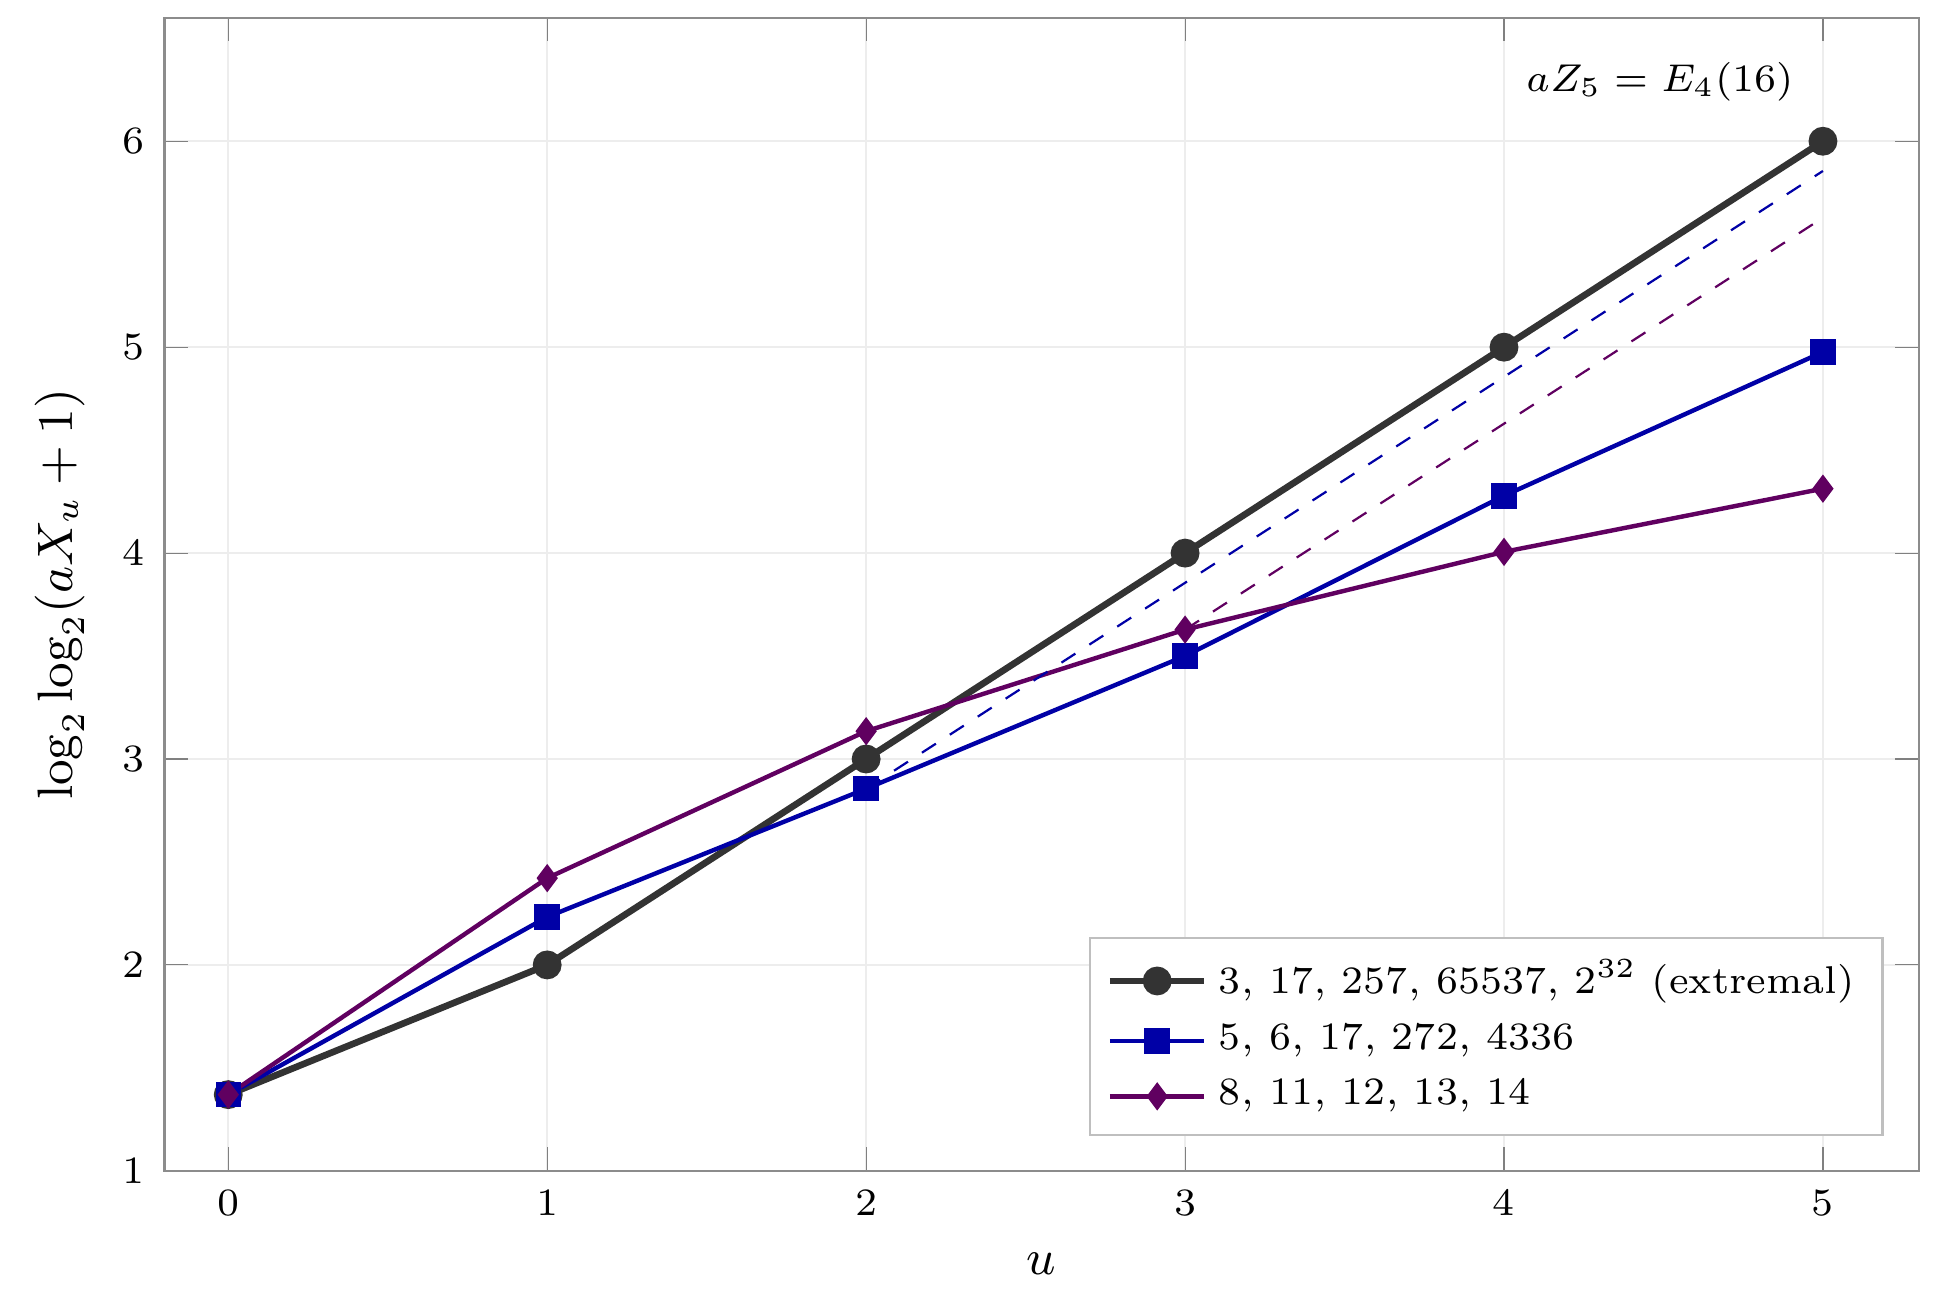
\includegraphics[width=0.86\textwidth]{figures/fig_dichotomy.png}
\caption{The proof of Theorem~\ref{thm:deficit} for $a/b=5/8$ and
$m=5$, on the scale $\log_2\log_2(aX_u+1)$. The extremal sequence
$3,17,257,65537,2^{32}$ rises by exactly $1$ per step from $u=1$ on and
ends at $aZ_5=E_4(16)$. The two other sequences satisfy \eqref{eq:hyp},
start above it, and fall below it at $u=2$ and $u=3$. From that point
Lemmas~\ref{lem:tail} and~\ref{lem:cn} give
$aX_5<(aX_u+1)^{2^{5-u}}$, the dashed line of slope $1$, which ends
below $E_4(16)$. A sequence that stayed above the extremal one up to
$u=4$ would end below it at $u=5$, by Lemma~\ref{lem:major}.}
\label{fig:dichotomy}
\end{figure}

\begin{proof}[Proof of Theorem~\ref{thm:deficit}]
Put $G=b(a+1)/d$, so that $G-1=a(b+1)/d$, and define real numbers
\[
  z_1=\frac{b+1}{d},\qquad z_u=G^{2^{u-2}}+1\quad(2\le u\le m-1),\qquad
  z_m=G^{2^{m-2}} .
\]
Then $aZ_1=G-1$, induction gives $aZ_u=G^{2^{u-1}}-1$ for
$1\le u\le m-1$, and $aZ_m=(G^{2^{m-2}}-1)G^{2^{m-2}}=E_{m-1}(G)$.
The numbers $z_2,\dots,z_m$ are the sequence of the proof of
Lemma~\ref{lem:cn} with $G-1$ in place of $a$ and $m-1$ terms, so by
\eqref{eq:zprod}
\[
  \prod_{u=1}^{m}\Bigl(1-\frac1{z_u}\Bigr)
  =\frac{a+1}{b+1}\cdot\frac{G-1}{G}
  =\frac{a+1}{b+1}\cdot\frac{a(b+1)}{b(a+1)}=\frac ab .
\]

Suppose first that $X_u\le Z_u$ for some $1\le u\le m-1$, so that
$aX_u+1\le G^{2^{u-1}}$. Lemmas~\ref{lem:tail} and~\ref{lem:cn},
applied to the $m-u\ge1$ terms $x_{u+1},\dots,x_m$, and
\eqref{eq:Ecomp} give
\[
  aX_m\le E_{m-u}(aX_u+1)\le E_{m-u}\bigl(G^{2^{u-1}}\bigr)
  =E_{m-1}(G).
\]
Otherwise $X_u>Z_u$ for all $u\le m-1$. If also $X_m>Z_m$, then
Lemma~\ref{lem:major}, which applies because every $z_u$ exceeds $1$
(for $z_1$ because $b+1>d$), gives
$\prod(1-1/x_i)>\prod(1-1/z_i)=a/b$, contrary to \eqref{eq:hyp}.
Hence $X_m\le Z_m$, that is $aX_m\le E_{m-1}(G)$.

If $d\mid b+1$, then $z_1$ is an integer greater than $1$, so
$z_1\ge2$, and $G-1=az_1$, $G\ge3$ and all $z_u$ are integers. They
are nondecreasing: $z_2\ge G\ge z_1$, since $G\ge z_1$ amounts to
$ab\ge1$; the middle terms increase; and for $m\ge3$ we have
$z_m=(z_{m-1}-1)^2\ge z_{m-1}$ because $z_{m-1}-1\ge G\ge3$. The
product of $1-1/z_u$ is $a/b$ over all $m$ terms and larger over the
first $m-1$, so the $z_u$ satisfy \eqref{eq:hyp} and attain
$aZ_m=E_{m-1}(G)$.
\end{proof}

\begin{figure}[t]
\centering
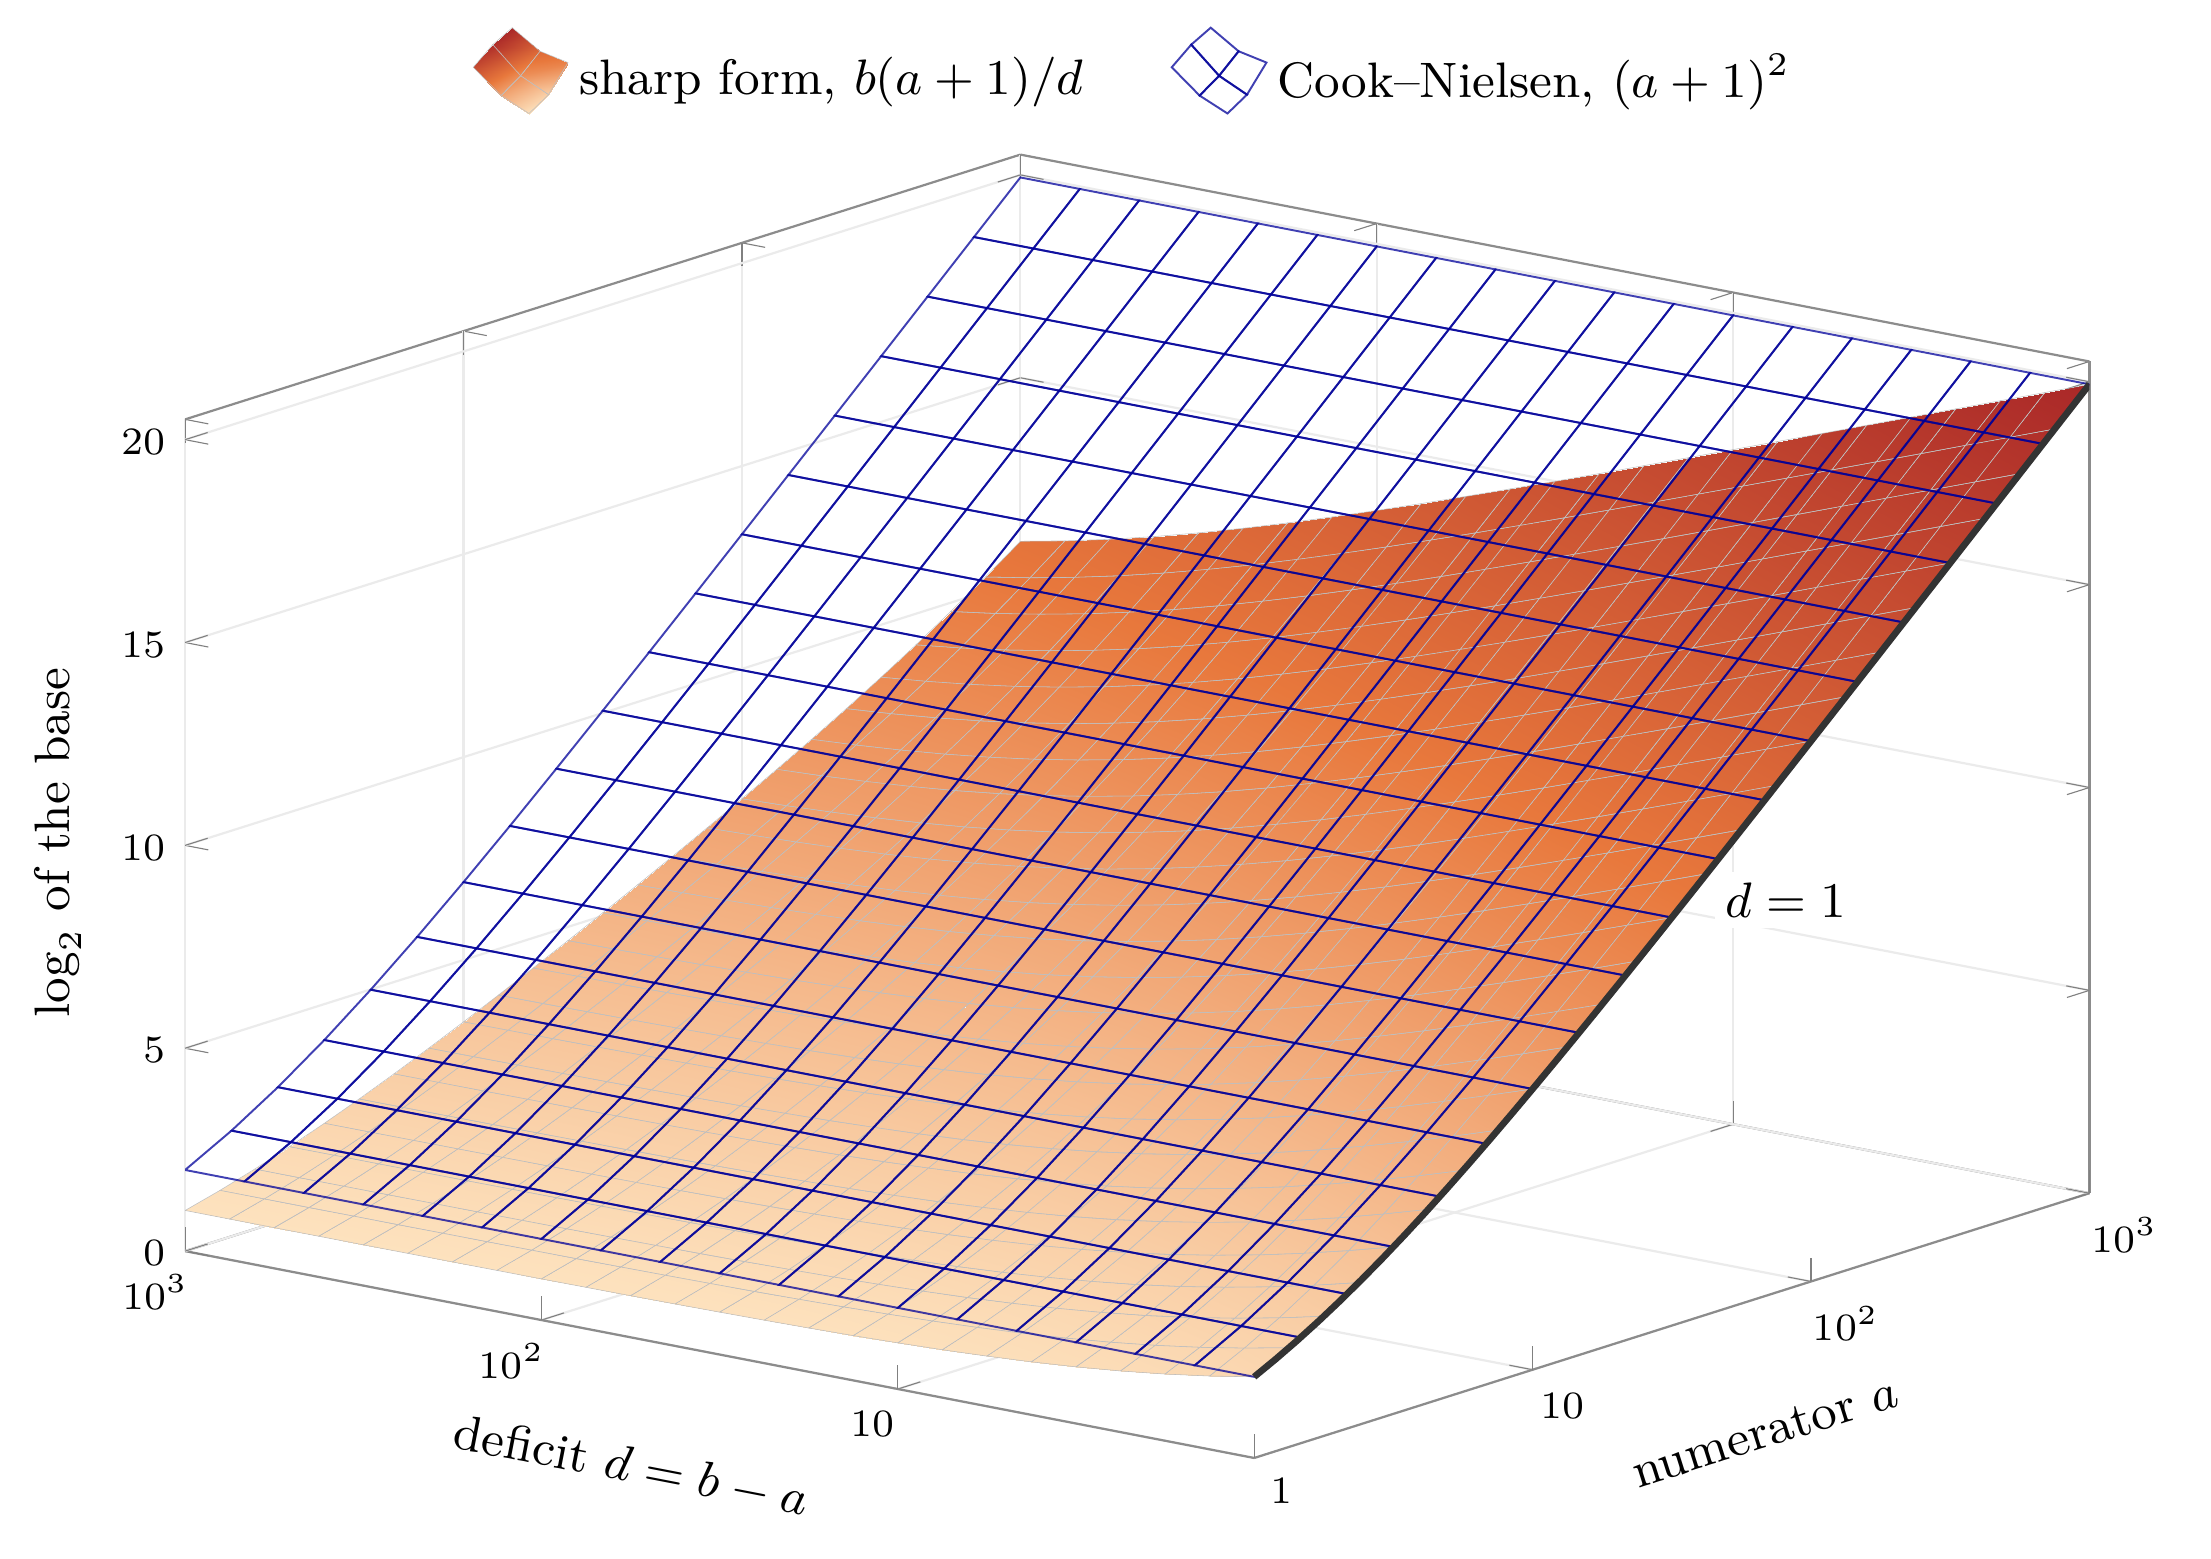
\includegraphics[width=0.94\textwidth]{figures/fig_bases.png}
\caption{The base of the bound for $aX_m$ written as
$E_{m-1}(\,\cdot\,)$, on a $\log_2$ scale, over the numerator $a$ and
the deficit $d=b-a$. The wire mesh is the base $(a+1)^2$ of the lemma
of Cook and Nielsen, the shaded sheet below it the base $b(a+1)/d$ of
Theorem~\ref{thm:deficit}. They meet along $d=1$, where the two bounds
coincide, and separate as $d$ grows.}
\label{fig:bases}
\end{figure}

\begin{remark}\label{rem:compare}
Since $G=(a+1)/(1-a/b)$, the bound of Theorem~\ref{thm:deficit}
depends on $b$ only through the distance of $a/b$ from $1$. Its base
is smaller than the base $(a+1)^2$ of Lemma~\ref{lem:cn} by the factor
$(a+1)d/b$, which is at least $1$ because $(a+1)d-b=a(d-1)\ge0$;
Figure~\ref{fig:bases} shows the two bases. Stone's bound
$E_{m-1}(b^2/d)$ exceeds ours by the factor $b/(a+1)$ in the base. In
the application below $a=A_j$ and $b=MB_j$, and then the base
$G=(A_j+1)/(1-P_j/M)$ decreases as $M$ increases, so the smallest
admissible value of $M$ yields an upper bound. The base
$b^2/d=M^2B_j^2/(MB_j-A_j)$ of Stone has no such property: it
decreases for $M<2P_j$ and increases for $M>2P_j$.
\end{remark}

\begin{remark}\label{rem:fermat}
The extremal sequences of Theorem~\ref{thm:deficit} are explicit. For
$a/b=5/8$ we have $d=3$, $z_1=3$ and $G=16$, and with $m=4$ the
sequence is $3,17,257,65536$:
\[
  \frac23\cdot\frac{16}{17}\cdot\frac{256}{257}\cdot\frac{65535}{65536}
  =\frac58,\qquad
  5\cdot3\cdot17\cdot257\cdot65536=2^{32}-2^{16}=E_3(16).
\]
The first three terms are Fermat primes. For $a=1$ the sequence of
the proof of Lemma~\ref{lem:cn} consists of the Fermat numbers
$F_0,\dots,F_{m-2}$ followed by $2^{2^{m-1}}$, and the products
$F_0F_1\cdots F_{r-1}=2^{2^r}-1$ with $1\le r\le5$ are the solutions
$3$, $15$, $255$, $65535$ and $4294967295$ of \eqref{eq:second} in
\eqref{eq:known}. Such products have $n/\varphi(n)$ just below $2$,
and so do the deepest nodes of the search of
Section~\ref{sec:sizesearch} (Section~\ref{sec:hard}).
\end{remark}

\subsection{Heavy solutions}\label{sec:heavy}
For $0\le j\le k-1$ put
\begin{equation}\label{eq:V}
  V_j=V_j(M)=\frac{MB_j(A_j+1)}{MB_j-A_j}=\frac{A_j+1}{1-P_j/M}.
\end{equation}
By Lemma~\ref{lem:sizefacts}(i) the denominator is positive, and
$V_j(M)$ decreases as $M$ increases.

\begin{proposition}\label{prop:sizebounds}
For $0\le j\le k-1$,
\[
  n<(A_j+1)^{2^{k-j}}\qquad\text{and}\qquad n<V_j^{\,2^{k-j-1}} .
\]
\end{proposition}

\begin{proof}
Take $m=k-j$, $x_i=p_{j+i}$, $a=A_j$ and $b=MB_j$. Then
\[
  \prod_{i=j+1}^{k}\Bigl(1-\frac1{p_i}\Bigr)=\frac{P_j}{P_k}
  <\frac{P_j}{M}=\frac ab<\frac{P_j}{P_{k-1}}
  =\prod_{i=j+1}^{k-1}\Bigl(1-\frac1{p_i}\Bigr)
\]
by Lemma~\ref{lem:sizefacts}(i), so \eqref{eq:hyp} holds, $a<b$, and
$ax_1\cdots x_m=n$. Lemma~\ref{lem:cn} gives $n\le E_{k-j}(A_j+1)$,
which implies the first bound. For $j\le k-2$,
Theorem~\ref{thm:deficit} gives $n\le E_{k-j-1}(V_j)$, because
$b(a+1)/d=V_j$. For $j=k-1$, Lemma~\ref{lem:sizefacts}(ii) gives
$n=A_{k-1}p_k<A_{k-1}MB_{k-1}/(MB_{k-1}-A_{k-1})<V_{k-1}$.
\end{proof}

\begin{definition}\label{def:heavy}
Let $s\ge0$ be an integer, and put $\theta_i=2^{2^{i-s}}$ for $i\ge s$
and $\theta_i=1$ for $i<s$. A composite solution $n$ of
\eqref{eq:first} is \emph{$s$-heavy} if for every $j$ with
$0\le j\le k-1$
\begin{enumerate}[label=\textup{(H\arabic*)}]
\item $A_j\ge\theta_j$, and
\item $V_j\ge\theta_{j+1}$.
\end{enumerate}
\end{definition}

\begin{corollary}\label{cor:light}
A composite solution of \eqref{eq:first} with $k$ prime factors that
is not $s$-heavy satisfies $n<2^{2^{k-s}}$.
\end{corollary}

\begin{proof}
If (H1) fails at $j$, then $j\ge s$ and $A_j+1\le2^{2^{j-s}}$, and
Proposition~\ref{prop:sizebounds} gives
$n<(A_j+1)^{2^{k-j}}\le2^{2^{k-s}}$. If (H2) fails at $j$, then
$j+1\ge s$ because $V_j>1$, and $n<V_j^{2^{k-j-1}}<2^{2^{k-s}}$.
\end{proof}

For $s=2$ condition (H1) alone contradicts
Lemma~\ref{lem:sizefacts}(i), and the argument can be carried out by
hand.

\begin{proposition}\label{prop:hand}
No composite solution of \eqref{eq:first} is $2$-heavy. Consequently
every composite solution with $k$ prime factors satisfies
$n<2^{2^{k-2}}$.
\end{proposition}

\begin{proof}
Let $n$ be $2$-heavy, and let $1\le i\le k-1$. Condition (H1) at $j=i$
and $A_i\le p_i^{\,i}$ give $p_i\ge\theta_i^{1/i}=2^{2^{i-2}/i}$. Hence
$p_7\ge24$, $p_8\ge256$, $p_9>19000$ and $p_i>4^i$ for $i\ge10$, so
that
\[
  \sum_{8\le i\le k-1}\frac1{p_i-1}<\frac1{256}+\frac1{19000}
  +\sum_{i\ge10}\frac1{4^i-1}<0.004 .
\]
Put $f(x)=x/(x-1)$, which decreases for $x>1$ and satisfies
$f(x)\le e^{1/(x-1)}$. Then $P_k=\prod_{i\le k}f(p_i)$ and
$f(p_k)<f(p_{k-1})$. Let $b_1,\dots,b_7$ be lower bounds for
$p_1,\dots,p_7$ and $\beta_j=\prod_{i\le j}f(b_i)$. If $k\le8$, then
$P_k<\beta_{k-1}f(b_{k-1})$. If $k\ge9$, the prime factors
$p_8,\dots,p_k$ contribute less than $e^{0.004}f(p_{k-1})<e^{0.008}$,
and $P_k<\beta_7e^{0.008}$. We distinguish four cases.
\begin{enumerate}[label=(\alph*)]
\item If $3\mid n$, then $p_1=3$ and $M\ge4$ by Lemma~\ref{lem:three},
  and the next prime factors are at least $5,7,11,13,17$ and, as
  $p_7\ge24$, $29$.
\item If $p_1=5$ and $p_2=7$, then no other prime factor is congruent
  to $1$ modulo $5$ or $7$ by Lemma~\ref{lem:basic}(ii), which excludes
  $11$, $29$ and $31$.
\item If $p_1=5$ and $p_2\ne7$, then $p_2\ge13$, and $11$ and $31$ are
  excluded because they are congruent to $1$ modulo $5$.
\item If $p_1\ge7$, the prime factors are at least the primes from $7$
  on, and $p_7\ge29$.
\end{enumerate}
In cases (b) to (d), $3\nmid n$ and $M\ge2$. Table~\ref{tab:hand}
lists the bounds $b_1,\dots,b_7$ in each case and the larger of
$\max_{j\le7}\beta_jf(b_j)$ and $\beta_7e^{0.008}$. In every case it is
less than $M$, so that $P_k<M$, contrary to
Lemma~\ref{lem:sizefacts}(i). Hence no composite solution is
$2$-heavy, and Corollary~\ref{cor:light} with $s=2$ gives the bound.
\end{proof}

\begin{table}[ht]
\centering
\caption{The four cases in the proof of Proposition~\ref{prop:hand}:
lower bounds $b_1,\dots,b_7$ for the seven smallest prime factors and
the resulting upper bound for $P_k$, rounded up.}
\label{tab:hand}
\smallskip
\small
\begin{tabular}{@{}llrr@{}}
\toprule
case & $b_1,\dots,b_7$ & bound for $P_k$ & $M\ge$ \\
\midrule
(a) $p_1=3$ & $3,5,7,11,13,17,29$ & $2.972$ & $4$ \\
(b) $p_1=5$, $p_2=7$ & $5,7,13,17,19,23,37$ & $1.957$ & $2$ \\
(c) $p_1=5$, $p_2\ne7$ & $5,13,17,19,23,29,37$ & $1.738$ & $2$ \\
(d) $p_1\ge7$ & $7,11,13,17,19,23,29$ & $1.749$ & $2$ \\
\bottomrule
\end{tabular}
\end{table}

The proof uses only condition (H1), whose failure gives the bound
through the lemma of Cook and Nielsen, and the fact that no prime
factor divides another minus one.
For $s=1$ the same argument needs only the cases $3\mid n$ and
$3\nmid n$, with the primes from $5$ on as lower bounds and
$p_6\ge41$, $p_7\ge569$, $p_8\ge65537$ from (H1); it shows that no
composite solution is $1$-heavy, which gives $n<2^{2^{k-1}}$, half the
number of binary digits allowed by the bound of Burek and \.Zmija. For larger $s$ the estimates of this proof
are too weak, and Theorem~\ref{thm:size}(i) follows once we know that
no solution is $7$-heavy, which Section~\ref{sec:sizesearch}
establishes with exact bounds at every node and with condition (H2)
and Theorem~\ref{thm:deficit} as well.

We first record how fast the prime factors of a heavy solution grow.
Fix $s$, an index $j\ge0$ and the product $A_j$ of $j$ odd primes. For
$i>j$ let $\lambda_i$ be the least positive integer $\lambda$ with
$A_j\lambda^{i-j}\ge\theta_i$, and put $y_i=(\theta_i/A_j)^{1/(i-j)}$.
Then $\lambda_i=\max\{1,\lceil y_i\rceil\}$, so $\lambda_i\ge y_i$,
and $\lambda_i<y_i+1$ whenever $\lambda_i>1$.

\begin{lemma}\label{lem:growth}
Let $i>j$.
\begin{enumerate}[label=\textup{(\roman*)}]
\item If $i\ge j+2$ and $y_i>1$, then $y_{i+1}\ge y_i^{4/3}$.
\item If $n$ is an $s$-heavy solution, $A_j$ is the product of its $j$
smallest prime factors and $i\le k-1$, then $p_i\ge\lambda_i$.
\end{enumerate}
\end{lemma}

\begin{proof}
(i) If $y_i>1$, then $\theta_i>A_j\ge1$, so $i\ge s$ and
$\theta_{i+1}=\theta_i^2$. Hence
\[
  (i+1-j)\log y_{i+1}=2\log\theta_i-\log A_j
  \ge2(\log\theta_i-\log A_j)=2(i-j)\log y_i ,
\]
so $\log y_{i+1}\ge\frac{2(i-j)}{i+1-j}\log y_i\ge\frac43\log y_i$,
since $i-j\ge2$ and $\log y_i>0$.

(ii) By (H1) at $i$, $\theta_i\le A_i\le A_jp_i^{\,i-j}$, so
$p_i\ge\lambda_i$.
\end{proof}

The search needs an upper bound for $P_k/P_j$ that uses only
$p_1,\dots,p_j$ and a lower bound for $p_{j+1}$. For an integer
$q\ge3$ and $i>j$ let $\pi_i(q)$ be the $(i-j)$-th smallest prime that
is at least~$q$, if this prime is less than $2\cdot10^7$, and
$\pi_i(q)=q+2(i-j-1)$ otherwise. Put
$b_i=\max\{\pi_i(q),\lambda_i\}$, let $i_0$ be the least index
$i\ge j+3$ with $\lambda_i>10^{30}$, and define
\begin{equation}\label{eq:Gamma}
  \Gamma_j(q)=\max\Bigl\{\frac{q}{q-1},\ \
  \max_{j+1\le i<i_0}\,\frac{b_i+2}{b_i+1}\prod_{l=j+1}^{i}
  \frac{b_l}{b_l-1},\ \
  \Bigl(1+\frac{16}{\lambda_{i_0}-2}\Bigr)\prod_{l=j+1}^{i_0-1}
  \frac{b_l}{b_l-1}\Bigr\}.
\end{equation}
The quantity $\Gamma_j(q)$ depends only on $j$, $A_j$, $q$ and $s$,
and it is a finite computation because $\lambda_i$ grows doubly
exponentially in~$i$.

\begin{lemma}\label{lem:ext}
Let $n$ be an $s$-heavy solution, $0\le j\le k-1$, and let $q$ be an
integer with $3\le q\le p_{j+1}$. Then $P_k\le P_j\Gamma_j(q)$.
\end{lemma}

\begin{proof}
The quotient $P_k/P_j$ is the product of $p_i/(p_i-1)$ over
$j<i\le k$, and $x/(x-1)$ decreases in $x$. For $j<i\le k-1$ we have
$p_i\ge\pi_i(q)$, since $p_{j+1}<\dots<p_i$ are odd primes at least
$q$, and $p_i\ge\lambda_i$ by Lemma~\ref{lem:growth}(ii); so
$p_i\ge b_i$. For the last prime, $p_k\ge q$ if $k=j+1$ and
$p_k\ge p_{k-1}+2\ge b_{k-1}+2$ otherwise. This bounds $P_k/P_j$ by
the first term of \eqref{eq:Gamma} when $k=j+1$, and by the second
term, with $i=k-1$, when $j+2\le k\le i_0$.

Suppose $k>i_0$. The primes $p_{j+1},\dots,p_{i_0-1}$ contribute at
most $\prod_{l=j+1}^{i_0-1}b_l/(b_l-1)$, as before. Put $Y=y_{i_0}$.
Since $\lambda_{i_0}>10^{30}$, we have $Y>\lambda_{i_0}-1\ge10^{30}$,
and Lemma~\ref{lem:growth} gives
$p_i\ge\lambda_i\ge y_i\ge Y^{(4/3)^{i-i_0}}$ for $i_0\le i\le k-1$.
As $p_k>p_{k-1}$, the factor of $p_k$ is at most that of $p_{k-1}$,
so
\[
  \prod_{i=i_0}^{k}\frac{p_i}{p_i-1}
  \le\prod_{i=i_0}^{k-1}\Bigl(1+\frac1{p_i-1}\Bigr)^{2}
  \le\exp\Bigl(2\sum_{u\ge0}\frac1{Y^{(4/3)^u}-1}\Bigr).
\]
Because $(4/3)^u\ge1+u/3$ and $Y\ge10^{30}$, the terms with $u\ge1$
add up to less than $1/(Y-1)$, so the exponent is less than
$4/(Y-1)\le1$. With $e^x\le1+2x$ for $0\le x\le1$ the product is at
most $1+8/(Y-1)<1+8/(\lambda_{i_0}-2)$, which is smaller than the
factor $1+16/(\lambda_{i_0}-2)$ of the third term of \eqref{eq:Gamma}.
\end{proof}

\subsection{The search}\label{sec:sizesearch}
Fix $s$. Let $S=(p_1,\dots,p_j)$, $j\ge0$, be an increasing sequence
of odd primes in which no $p_i$ divides any $p_l-1$, and write $A_j$,
$B_j$ and $P_j$ as before. Let $\mu(S)$ be the least integer $M>P_j$
with $M\ge2$ and, if $p_1=3$, $M\equiv1\pmod3$, and let $\mu'(S)$ be
the next such integer. We say that a solution $n$ \emph{extends} $S$
if $j\le k-1$ and $S$ consists of the $j$ smallest prime factors
of~$n$. By Lemmas~\ref{lem:basic}, \ref{lem:three}
and~\ref{lem:sizefacts}(i), the quotient $M$ of such an $n$ satisfies
$M\ge\mu(S)$. For $M>P_j$ we use $V_j(M)$ as in \eqref{eq:V},
computed from $S$.

The tree $\mathcal T_s$ is built from the empty sequence by the
following rules, applied to each sequence $S$ of length $j$ that is
generated; Figure~\ref{fig:rules} summarises them.

\begin{enumerate}[label=\textup{(R\arabic*)},leftmargin=*]
\item\label{r:ratio} \emph{Ratio test.} Let $q_1$ be the least prime
greater than $p_j$ ($q_1=3$ if $j=0$). If $P_j\Gamma_j(q_1)\le\mu(S)$,
the sequence $S$ is discarded.
\item\label{r:deficit} \emph{Deficit test.} If
$V_j(\mu(S))<\theta_{j+1}$, the sequence $S$ is discarded.
\end{enumerate}
A sequence that survives both tests is a \emph{node} of
$\mathcal T_s$. At a node:
\begin{enumerate}[label=\textup{(R\arabic*)},leftmargin=*,resume]
\item\label{r:last} \emph{Last prime.} If $j\ge1$, then for each
integer $M$ with $\mu(S)\le M<P_j(p_j+2)/(p_j+1)$, and
$M\equiv1\pmod3$ if $p_1=3$, test whether
$(MB_j-1)/(MB_j-A_j)$ is a prime greater than $p_j$ that is not $1$
modulo any $p_i$.
\item\label{r:children} \emph{Children.} Put $\mu=\mu(S)$ and
$q_c=\lfloor\mu B_j/(\mu B_j-A_j)\rfloor$. Generate the sequences
$(p_1,\dots,p_j,q)$ for the primes $q>p_j$ with
$q\not\equiv1\pmod{p_i}$ for $i\le j$ and with $A_jq\ge\theta_{j+1}$,
taking $q$ in increasing order and omitting~$q$ in the following
cases.
\begin{enumerate}[label=(\roman*)]
\item If $P_j\Gamma_j(q)\le\mu$, omit $q$ and every larger prime.
\item If $q\le q_c$ and $P_j\Gamma_j(q)\le\mu'(S)$, omit every prime
in $[q,q_c]$.
\item If $q>q_c$ and $V_{j+1}(\mu)$, computed for the sequence
$(p_1,\dots,p_j,q)$, is less than $\theta_{j+2}$, omit $q$.
\end{enumerate}
\end{enumerate}

A prime $q$ satisfies $q\le q_c$ exactly when $P_jq/(q-1)\ge\mu$, so
in (ii) a solution extending $(p_1,\dots,p_j,q)$ has $P_{j+1}\ge\mu$
and hence $M\ge\mu'(S)$. For $q>q_c$ we have $P_{j+1}<\mu$, so
$V_{j+1}(\mu)$ is defined, and after multiplication by its positive
denominator the inequality in (iii) becomes a quadratic inequality in
$q$ with positive leading coefficient;\footnote{With $D=\mu B_j-A_j$
and $\theta=\theta_{j+2}$ one has $V_{j+1}(\mu)=\mu B_j(q-1)(A_jq+1)/(Dq-\mu
B_j)$, and $V_{j+1}(\mu)<\theta$ reads
$\mu A_jB_jq^2+\bigl(\mu B_j-\mu A_jB_j-\theta D\bigr)q+(\theta-1)\mu
B_j<0$.} the primes omitted by (iii)
therefore form an interval, which is computed once per node.

\begin{figure}[t]
\centering
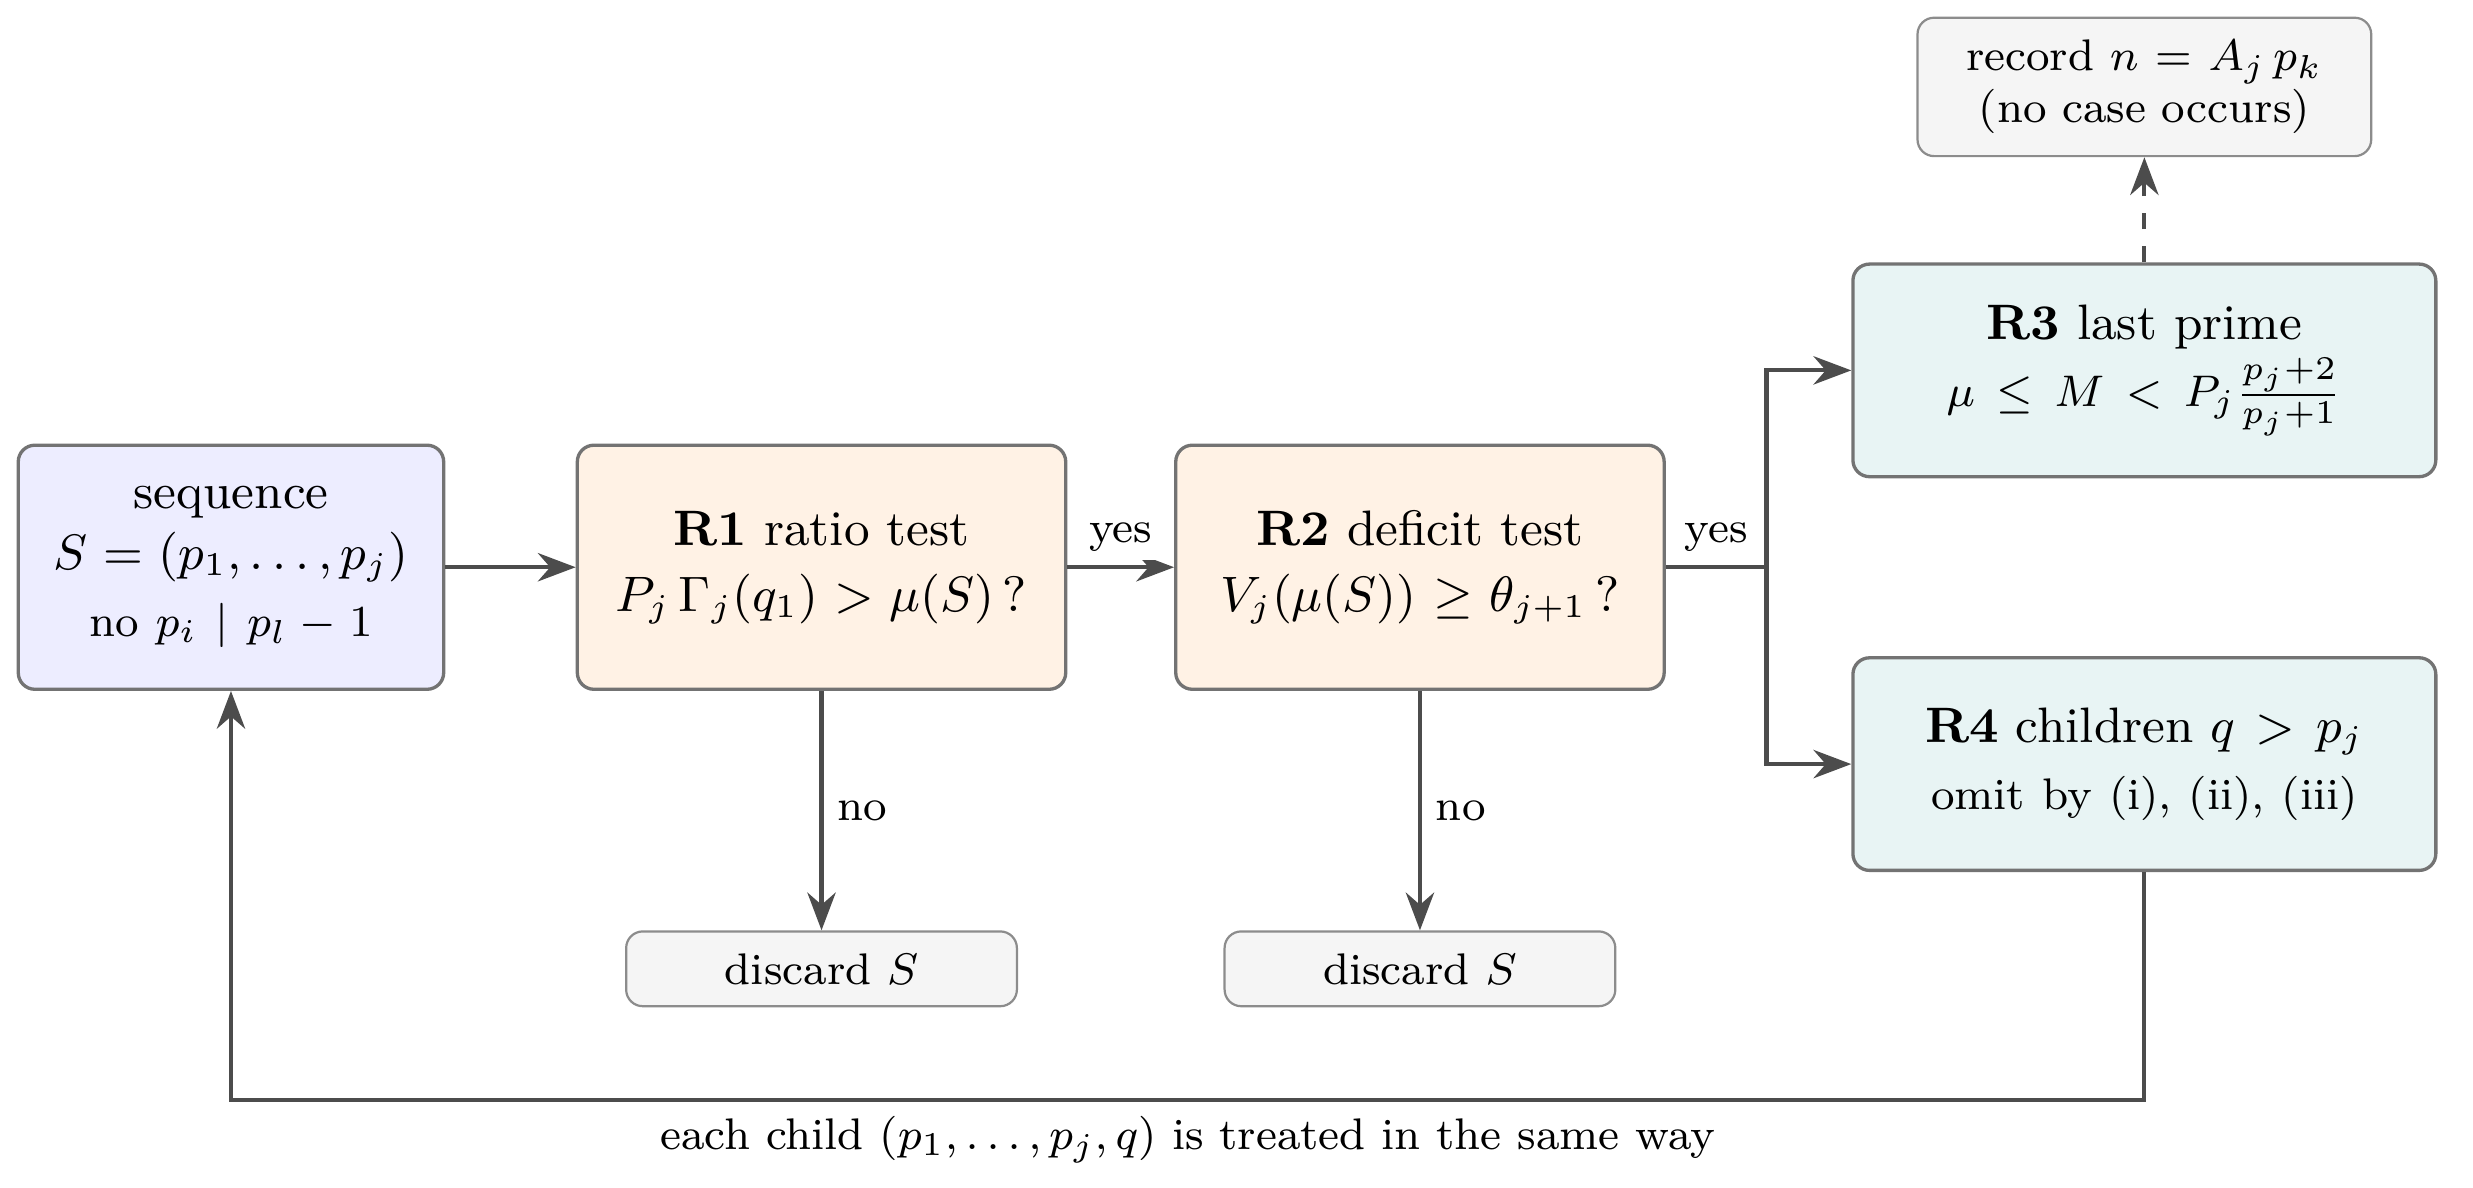
\includegraphics[width=0.96\textwidth]{figures/fig_rules.png}
\caption{The treatment of a sequence $S=(p_1,\dots,p_j)$ in the tree
$\mathcal T_s$. A sequence that fails the ratio test or the deficit
test cannot be extended by an $s$-heavy solution. A node is tested for
a last prime factor and passes to its children every prime that the
three omission rules allow.}
\label{fig:rules}
\end{figure}

\begin{proposition}\label{prop:sizecomplete}
Let $n$ be an $s$-heavy solution. Then $(p_1,\dots,p_{k-1})$ is a
node of $\mathcal T_s$, and rule~\ref{r:last} at that node finds
$p_k$.
\end{proposition}

\begin{proof}
Write $S_j=(p_1,\dots,p_j)$. We show by induction on $j$ that $S_j$
is generated and is a node, for $0\le j\le k-1$. The empty sequence
$S_0$ is generated by definition. Suppose that $S_j$ is generated. As
$n$ extends $S_j$, we have $M\ge\mu(S_j)$. Lemma~\ref{lem:ext} with
$q=q_1\le p_{j+1}$ gives $P_j\Gamma_j(q_1)\ge P_k>M\ge\mu(S_j)$, so
\ref{r:ratio} does not discard $S_j$, and
$V_j(\mu(S_j))\ge V_j(M)\ge\theta_{j+1}$ by (H2), so \ref{r:deficit}
does not either. Thus $S_j$ is a node.

Now let $j\le k-2$. The prime $p_{j+1}$ is a candidate of
\ref{r:children} at $S_j$, by Lemma~\ref{lem:basic}(ii) and (H1) at
$j+1$. Lemma~\ref{lem:ext} gives $P_j\Gamma_j(q)\ge P_k>M\ge\mu(S_j)$
for every integer $q$ with $3\le q\le p_{j+1}$, so rule (i) applies
at no prime $q\le p_{j+1}$. If $p_{j+1}\le q_c$, then
$P_{j+1}\ge\mu(S_j)$, and $M>P_{j+1}$ forces $M\ge\mu'(S_j)$; hence
$P_j\Gamma_j(q)>\mu'(S_j)$ for $q\le p_{j+1}$, rule (ii) applies at no
prime $q\le p_{j+1}$, and an application at a larger prime does not
reach $p_{j+1}$. If $p_{j+1}>q_c$, rule (ii) omits only primes up to
$q_c$, and $V_{j+1}(\mu(S_j))\ge V_{j+1}(M)\ge\theta_{j+2}$ by (H2) at
$j+1$, so rule (iii) does not omit $p_{j+1}$. Hence $S_{j+1}$ is
generated.

At the node $S_{k-1}$ we have $\mu(S_{k-1})\le M<P_k$ and
$P_k=P_{k-1}p_k/(p_k-1)\le P_{k-1}(p_{k-1}+2)/(p_{k-1}+1)$, so $M$ is
one of the values tested in \ref{r:last}, and $p_k$ is the quotient
given by Lemma~\ref{lem:sizefacts}(ii).
\end{proof}

\subsection{The computation}\label{sec:sizecomp}
All quantities in the rules are rational numbers, and the search
evaluates them exactly. The primes $\pi_i(q)$ below $2\cdot10^7$ are
taken from a sieve. Primes above that are reached by stepping to the
next probable prime; such a step never skips a prime, so a composite
number may occasionally be treated as a prime, which can only enlarge
the tree. It is equally harmless to replace $q_1$ in \ref{r:ratio} by
the smaller number $p_j+2$, as one of the two programs of
Appendix~\ref{app:size} does beyond the sieve, because the proof of
Proposition~\ref{prop:sizecomplete} uses only Lemma~\ref{lem:ext},
which holds for every integer $q$ with $3\le q\le p_{j+1}$. In
rule~\ref{r:last} the quotient was never an integer, so no primality
proof is needed.

\begin{table}[ht]
\centering
\caption{The tree $\mathcal T_7$ by depth $j$: the number of nodes and
the number of values of $M$ tested by rule~\ref{r:last}.}
\label{tab:heavy}
\smallskip
\small
\begin{tabular}{@{}l*{14}{r}@{}}
\toprule
$j$ & 0 & 1 & 2 & 3 & 4 & 5 & 6 & 7 & 8 & 9 & 10 & 11 & 12 & 13\\
\midrule
nodes & 1 & 1 & 1 & 3 & 6 & 7 & 7 & 13 & 31 & 79 & 266 & 1\,501 & 29\,073 & 2\,689\\
tests & 0 & 0 & 0 & 0 & 0 & 0 & 0 & 0 & 0 & 0 & 16 & 215 & 11\,894 & 2\,689\\
\bottomrule
\end{tabular}
\end{table}

\begin{theorem}\label{thm:sizesearch}
The tree $\mathcal T_7$ has $33678$ nodes and depth $13$.
Rule~\ref{r:last} tests $14814$ values of $M$, and for none of them is
the quotient $(MB_j-1)/(MB_j-A_j)$ an integer. Consequently, by
Proposition~\ref{prop:sizecomplete}, no composite solution of
\eqref{eq:first} is $7$-heavy.
\end{theorem}

Table~\ref{tab:heavy} lists the nodes by depth. Every node has
$\mu(S)=2$, so every node has $p_1\ne3$ and $P_j<2$; in particular
the sequence $(3)$, for which $\mu=4$, is discarded at once by the
ratio test. The first branch of the tree is
$5,7,13,17,19,23,37,59,67,73$, the beginning of the independent set
of Section~\ref{sec:indep} chosen one prime at a time, and the deepest
nodes have thirteen entries.

\begin{proof}[Proof of Theorem~\textup{\ref{thm:size}(i)}]
By Theorem~\ref{thm:sizesearch} no composite solution of
\eqref{eq:first} is $7$-heavy, and Corollary~\ref{cor:light} with
$s=7$ gives $n<2^{2^{k-7}}$.
\end{proof}

For $s=1,\dots,7$ the trees $\mathcal T_s$ have $1$, $3$, $7$, $12$,
$24$, $118$ and $33678$ nodes. The deficit test does most of the work:
without rules~\ref{r:deficit} and (iii), the tree $\mathcal T_6$
already has $4469$ nodes and depth $12$.

\begin{figure}[t]
\centering
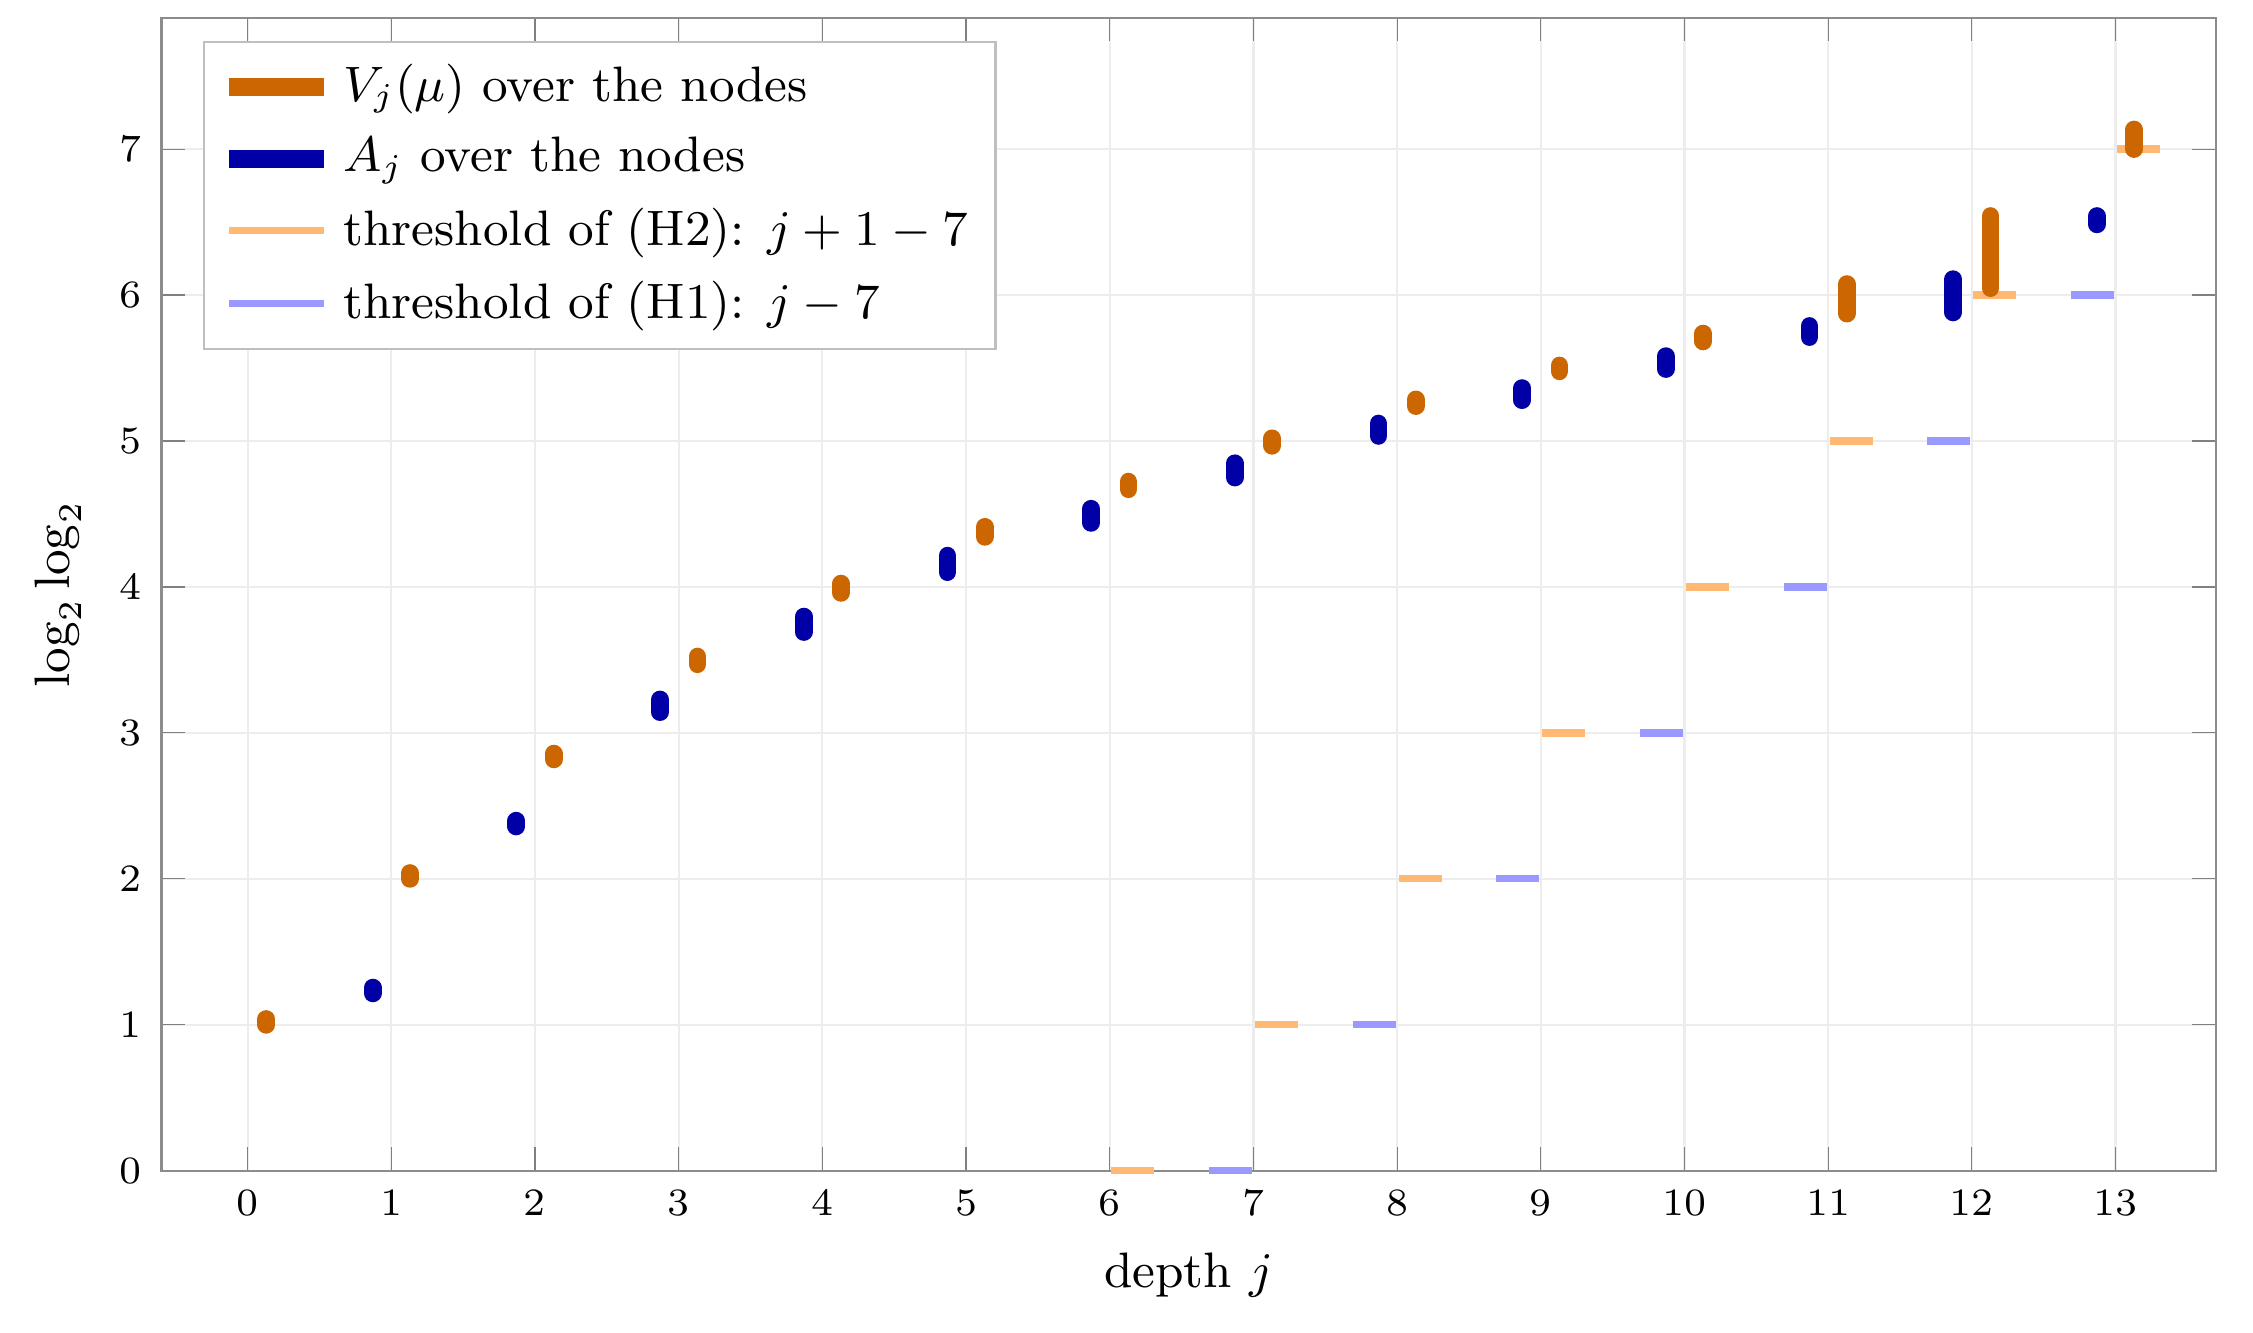
\includegraphics[width=0.94\textwidth]{figures/fig_margins.png}
\caption{The nodes of $\mathcal T_7$ by depth $j$. The bars span the
range of $\log_2\log_2 V_j(\mu)$ (right of each depth) and of
$\log_2\log_2 A_j$ (left of each depth) over the nodes of depth $j$,
and the short marks below them are the thresholds $j+1-7$ of (H2) and
$j-7$ of (H1). The deficit condition (H2) is the one that binds: at
depth $13$ the smallest value of $\log_2\log_2V_{13}$ is
$7.0000075\ldots$}
\label{fig:margins}
\end{figure}

\subsection{Larger quotients}\label{sec:large}
When $M\ge3$, condition (H1) for a suitable $s$ is incompatible with
Lemma~\ref{lem:sizefacts}(i) and the bounds of
Section~\ref{sec:indep}, and no further search is needed. Let
$\ell_1<\ell_2<\cdots$ be integers with $p_i\ge\ell_i$ for $i\le k$,
let $J\ge1$, and let $V^*$ be a number with $P_{\min\{k,J\}}<V^*$. If
(H1) holds for all $j\le k-1$, then $A_i\le p_i^{\,i}$ gives
$p_i\ge\rho_i$ for $i\le k-1$, where $\rho_i$ is the least positive
integer $x$ with $x^i\ge\theta_i$. With $w_i=\max\{\ell_i,\rho_i\}$
we obtain, as in the proof of Lemma~\ref{lem:ext},
\begin{equation}\label{eq:R}
  P_k<R_s=V^*\max\Bigl\{1,\ \max_{J\le i<i_0}\,
  \frac{w_i'+2}{w_i'+1}\prod_{l=J+1}^{i}\frac{w_l}{w_l-1}
  \ ,\ \Bigl(1+\frac{16}{\rho_{i_0}-2}\Bigr)\prod_{l=J+1}^{i_0-1}
  \frac{w_l}{w_l-1}\Bigr\},
\end{equation}
where $w_i'=\max\{w_i,\ell_{i+1}-2\}$ accounts for
$p_{i+1}\ge\max\{\ell_{i+1},w_i+2\}$, and $i_0\ge\max\{J+1,s+4\}$ is
an index with $\rho_{i_0}>10^{30}$. The three terms cover $k\le J$,
then $J<k\le i_0$ with $k=i+1$, and $k>i_0$. The tail estimate is that
of Lemma~\ref{lem:ext}, applied to $y_i=\theta_i^{1/i}$, for which
$p_i\ge\rho_i\ge y_i>\rho_i-1$ when $\rho_i>1$, and
$\log y_{i+1}=\frac{2i}{i+1}\log y_i\ge\frac43\log y_i$ when
$i\ge\max\{s,2\}$. We evaluate $R_s$ in exact rational arithmetic, with
integer lower bounds in place of the $\rho_i$, which can only enlarge
it.

\begin{proof}[Proof of Theorem~\textup{\ref{thm:size}(ii)} and
\textup{(iii)}]
Suppose $3\mid n$. Then $M\ge4$, every prime factor other than $3$ is
congruent to $2$ modulo $3$, by Lemma~\ref{lem:three}, and
$k\ge10^8+2$ by Corollary~\ref{cor:indep}(ii). Take $J=10^8+1$,
$\ell_i=2i+1$, which is at most the $i$-th odd prime, and
$V^*=4(1-10^{-6})$. The $J$ smallest prime factors are $3$ and an
independent set of $10^8$ primes $p\equiv2\pmod3$, so
$P_J<\frac32\cdot\frac83(1-10^{-6})=V^*$ by
Proposition~\ref{prop:indep}(ii). The computation gives
$R_{10^8}=3.9999966\ldots<4$. If (H1) held for all $j\le k-1$ with
$s=10^8$, then \eqref{eq:R} would give $P_k<4\le M$, contrary to
Lemma~\ref{lem:sizefacts}(i). So $n$ is not $10^8$-heavy, and
Corollary~\ref{cor:light} gives (iii).

Suppose $M\ge3$ and $3\nmid n$. Then $k\ge16001$ by
Corollary~\ref{cor:indep}(i). Take $J=16000$, $\ell_i=r_i$, the primes
from $5$ on, and $V^*=2.999999$; the $J$ smallest prime factors form an
independent set, so $P_J<V^*$ by Proposition~\ref{prop:indep}(i).
Then $R_{15981}=2.99999900041\ldots<3$, and the same argument gives
$n<2^{2^{k-15981}}$. If $M\ge3$ and $3\mid n$, part (iii) gives a
stronger bound.
\end{proof}

The exponent $15981$ is the largest that this argument gives with
$J=16000$, since $R_{15982}=3.000016\ldots$. Everything is decided by
the prime factors around the $16000$-th. For $s=15981$, (H1) at
$j=16000$ gives $p_{16000}\ge\rho_{16000}>7\cdot10^9$, so that the
remaining prime factors raise $P_{16000}<2.999999$ by a factor less
than $1+10^{-9}$. For $s=15982$ the corresponding bound
$\rho_{16000}<10^5$ lies below $r_{16000}=176089$, and the next prime
factor alone may raise the product by the factor $1+1/176122$.

\subsection{Where the search is hard}\label{sec:hard}
The nodes that survive longest are prefixes with $P_j$ just below $2$,
the same kind of prefix that makes the next cases of
Section~\ref{sec:walls} expensive. Every node at depth $13$ has
$2-P_{13}<10^{-10}$: there $A_{13}$ has between $27$ and $29$ digits,
while $C_{13}=2B_{13}-A_{13}$ has between $14$ and $18$. In this
respect the deep nodes behave like the products of Fermat primes of
Remark~\ref{rem:fermat}, for which $2\varphi(n)-n=1$. For such a
prefix $1-P_j/2$ is tiny, so $V_j$ is large and the deficit test
cannot discard it. Its children are few for the same reason: a prime
$q\le q_c=\lfloor1/(1-P_j/2)\rfloor$, which exceeds $3\cdot10^{10}$ at
depth $13$, would raise $P_{j+1}$ to $2$ or more and force $M\ge3$, and
rule (ii) removes these primes. Figure~\ref{fig:margins} shows how
close to the threshold of (H2) the deepest nodes come.

The tree grows quickly with $s$ (Figure~\ref{fig:trees}), and for
$s=7$ more than nine tenths of its nodes lie at depths $12$ and $13$. Each further unit of $s$ halves the number of binary digits
allowed by Theorem~\ref{thm:size}(i). The method proves
$n<2^{2^{k-s}}$ for every $s$ for which the tree $\mathcal T_s$ can be
searched, and the cost of the search is dominated by the deep prefixes
with $P_j$ close to $2$. We have not completed the search for $s=8$:
at the node $5,7,13,17,19,23,37,59,67,73,317,5483$ of depth $12$,
where $2/P_{12}-1=7.0\cdot10^{-8}$, rule~\ref{r:children} already
generates more than $10^6$ sequences.

\begin{figure}[t]
\centering
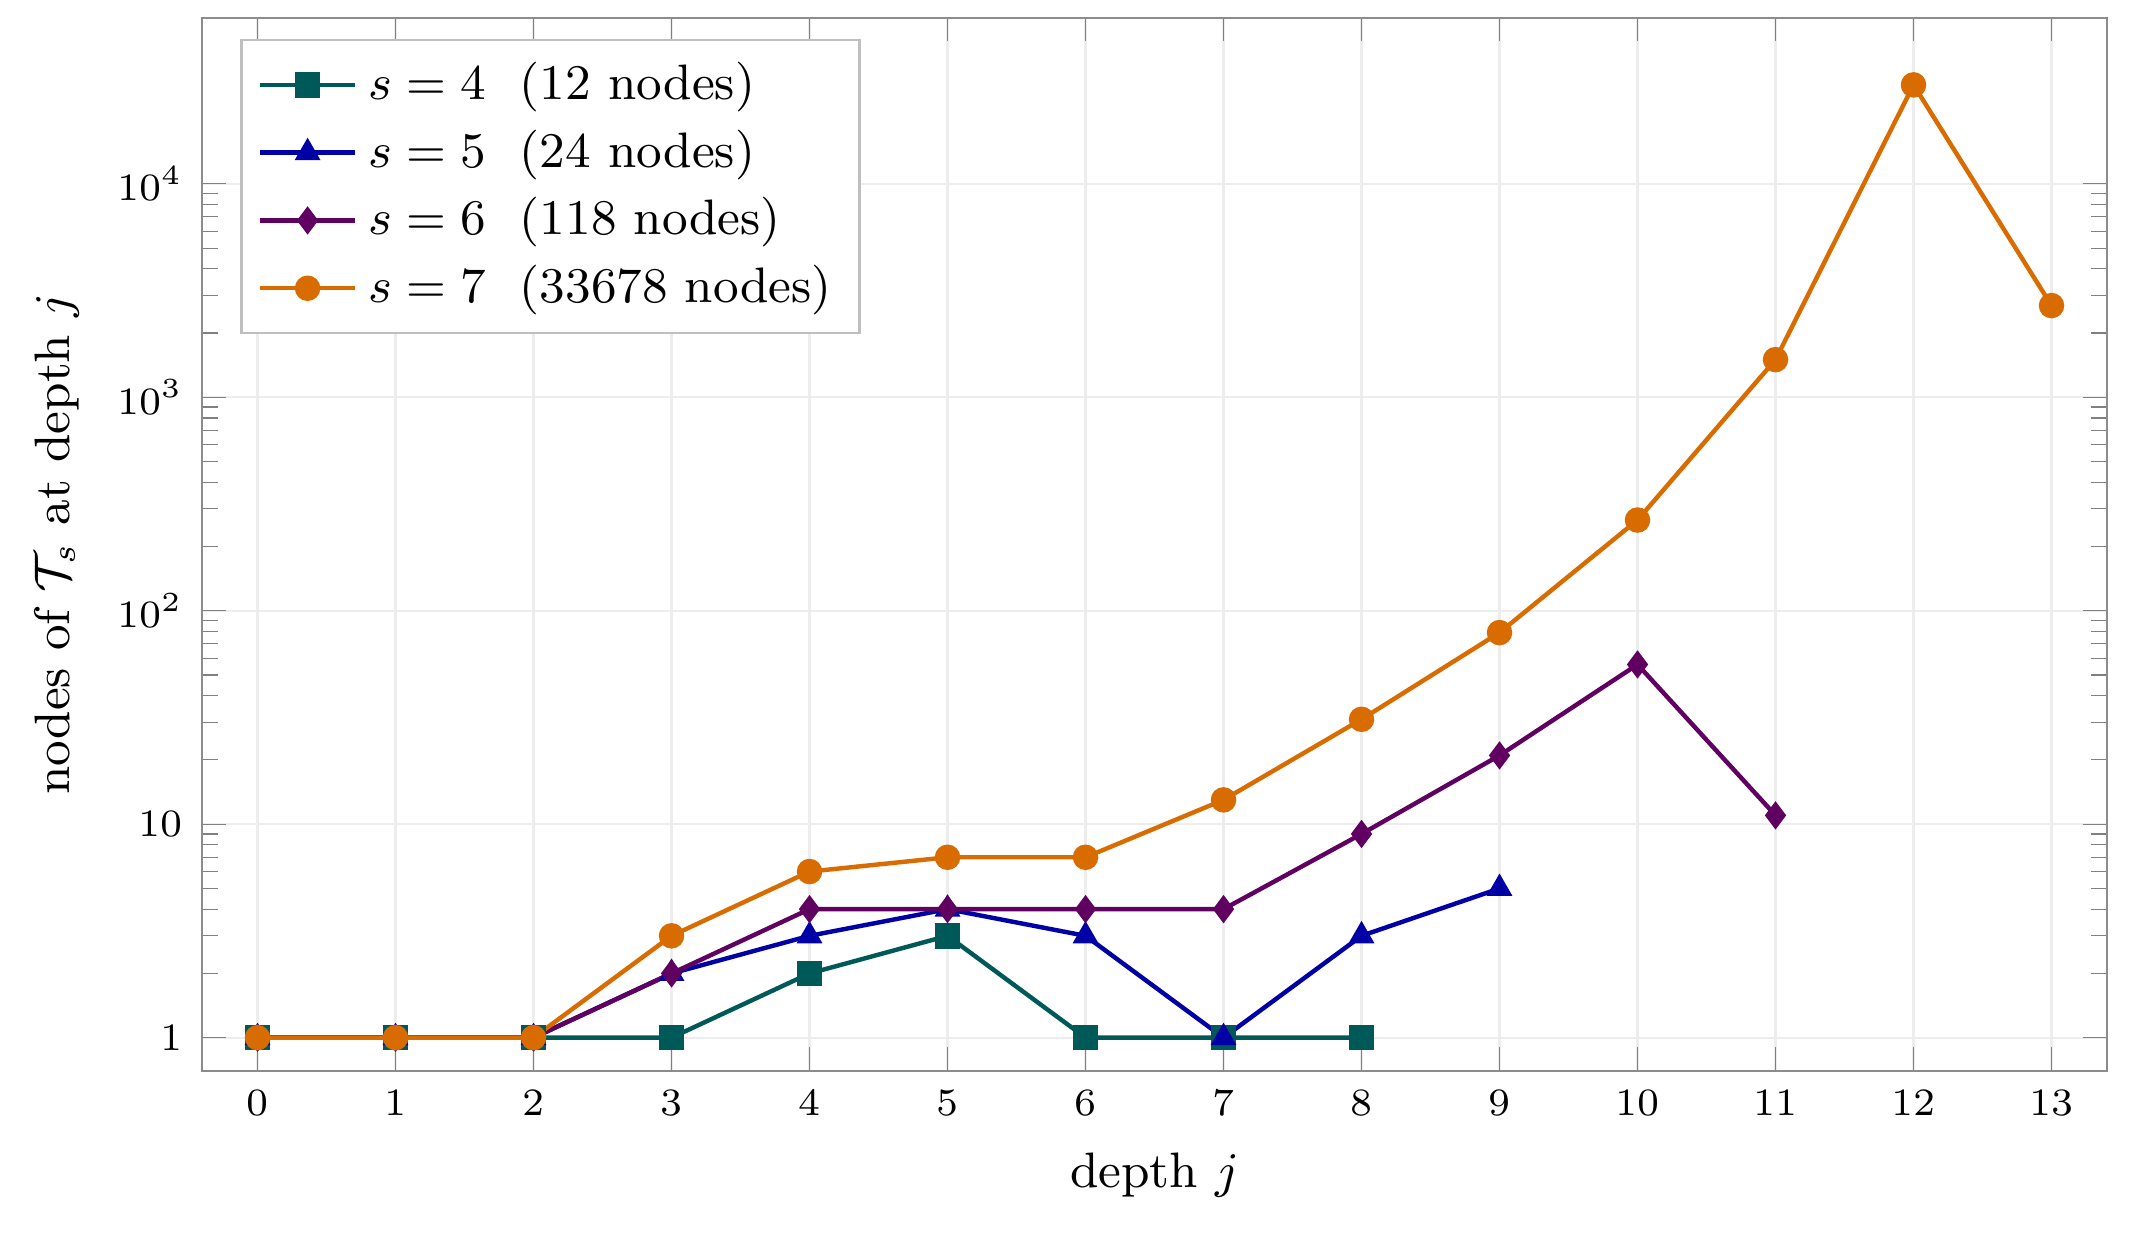
\includegraphics[width=0.86\textwidth]{figures/fig_trees.png}
\caption{The number of nodes of $\mathcal T_s$ at each depth, for
$s=4,5,6,7$, on a logarithmic scale.}
\label{fig:trees}
\end{figure}

\subsection{Comparison with other bounds}
Stone \cite[(52), (53)]{Sto24} treated tuples of primes with
$\prod(1-1/p_i)\le\frac12<\prod_{i<k}(1-1/p_i)$, which include the
prime factors of solutions with $M=2$. For $p_1=5$ he obtained
$\prod p_i\le E_k(\beta)$ with $\beta\approx1.66127$, and with
$\beta\approx1.50188$ when also $p_2=7$. Theorem~\ref{thm:size}(i)
gives the base $2^{1/128}=1.00543\ldots$ for solutions of
\eqref{eq:first}. Table~\ref{tab:bases} compares, along the first
branch of $\mathcal T_7$, the exponents $e$ for which the three bases
give $n<2^{2^{k-e}}$. The deficit gains about three quarters of a unit
of $e$ over Lemma~\ref{lem:cn}, and Theorem~\ref{thm:deficit} adds a
further gain over Stone's form that is largest for short prefixes.

\begin{table}[ht]
\centering
\caption{Along the branch $5,7,13,\dots$ of $\mathcal T_7$ with
$M=2$: the exponent $e$ such that the bound for $n$ obtained at depth
$j$ is $2^{2^{k-e}}$, for the base $(A_j+1)^2$ of Lemma~\ref{lem:cn},
the base $b^2/d$ of Stone and the base $V_j$ of
Theorem~\ref{thm:deficit}.}
\label{tab:bases}
\smallskip
\small
\begin{tabular}{@{}rrrrrr@{}}
\toprule
$j$ & $p_j$ & $P_j$ & Cook--Nielsen & Stone & Theorem~\ref{thm:deficit}\\
\midrule
1 & 5 & 1.25000 & $-0.370$ & $-0.142$ & $0.000$\\
2 & 7 & 1.45833 & $-0.370$ & $0.099$ & $0.181$\\
3 & 13 & 1.57986 & $-0.143$ & $0.486$ & $0.530$\\
4 & 17 & 1.67860 & $0.309$ & $1.017$ & $1.041$\\
5 & 19 & 1.77186 & $0.899$ & $1.644$ & $1.657$\\
6 & 23 & 1.85240 & $1.561$ & $2.324$ & $2.330$\\
7 & 37 & 1.90385 & $2.251$ & $3.030$ & $3.033$\\
8 & 59 & 1.93668 & $2.965$ & $3.759$ & $3.761$\\
9 & 67 & 1.96602 & $3.720$ & $4.516$ & $4.517$\\
10 & 73 & 1.99333 & $4.507$ & $5.265$ & $5.265$\\
\bottomrule
\end{tabular}
\end{table}

%%==================================================================
\section{The companion equation}\label{sec:second}
%%==================================================================

\subsection{Up to seven prime factors}\label{sec:seven}
Let $n$ satisfy \eqref{eq:second} with $\omega(n)\le7$. If $n\le3$
there is nothing to prove. Otherwise $n$ is odd, squarefree and
composite by Lemma~\ref{lem:basic}, and $n+1=2\varphi(n)$ by
Corollary~\ref{cor:seven}. Since $3$ may divide $n$, the search now
starts from $p_{\min}=3$, and we run it with $\varepsilon=+1$ for
$2\le k\le7$. The outcome is in Table~\ref{tab:seven}.

\begin{table}[ht]
\centering
\caption{The search for $n+1=2\varphi(n)$ with $3\le p_1$ and $k\le7$.}
\label{tab:seven}
\smallskip
\begin{tabular}{@{}rrrrl@{}}
\toprule
$k$ & nodes & terminal & largest width for $p_{k-1}$ & solutions found \\
\midrule
2 &     1 &     1 &                 1 & $15$ \\
3 &     3 &     2 &                 2 & $255$ \\
4 &     5 &     2 &                15 & $65535$ \\
5 &    11 &     4 &               256 & $83623935$, $4294967295$ \\
6 &    60 &    44 &            65\,536 & $6992962672132095$ \\
7 & 6\,914 & 6\,826 &          $2^{32}$ & none \\
\bottomrule
\end{tabular}
\end{table}

For $k\le6$ the search returns exactly the known solutions, each at
its own depth, and this is also a test of the programs. For $k=7$ it
returns nothing. Here the enumeration route is too slow, because one
terminal node, the prefix $3,5,17,257,65537$, has an interval for
$p_6$ of width $2^{32}$; for this prefix $C=1$ and
$D=2AB+C=2^{64}-2^{32}+1$, which is prime\footnote{Indeed
$A=2^{32}-1$, $B=2^{31}$ and $C=2B-A=1$, so
$D=2^{32}(2^{32}-1)+1=\Phi_6(2^{32})$, the sixth cyclotomic polynomial
at $2^{32}$. Its primality is well known and is confirmed by a
deterministic test, since $D<3.3\cdot10^{24}$.}. We
therefore use the divisor route throughout, which is rigorous in this
range: the largest integer $D$ factored in the case $k\le7$ has $21$
digits, so every factorisation is certified. For $k\le6$ the
enumeration route was also run and agrees node for node. This proves
Theorem~\ref{thm:eight} for solutions with at most seven prime
factors; the case of eight is treated in Section~\ref{sec:eight}.

\subsection{Solutions prime to three}
Let $n>3$ satisfy \eqref{eq:second} with $3\nmid n$ and
$\omega(n)\le15$. Then $n=p_1\cdots p_k$ with $5\le p_1$, and
$n+1=2\varphi(n)$ by Lemma~\ref{lem:Mtwo}. For $k\le6$ the product
$\prod p_i/(p_i-1)$ is at most $1.9490\ldots$, whereas
\eqref{eq:excess} requires it to be $2-1/\varphi(n)$. For $k\ge2$
this is at least $2-\frac1{24}>1.95$, as $\varphi(n)\ge4\cdot6$, and
for $k=1$ it is at least $\frac74$, whereas $p_1/(p_1-1)\le\frac54$. For
$7\le k\le14$ we ran both implementations with $\varepsilon=+1$ and
$p_{\min}=5$. Neither found a solution, and the node counts, the
numbers of terminal nodes and the largest widths coincide with those
of Table~\ref{tab:first} for every $k$. For $k=15$ the nodes at depth
$12$ and their intervals are again those of
Section~\ref{sec:fifteen}, and the method of Section~\ref{sec:three},
run with $\varepsilon=+1$ by both implementations and by the route of
Section~\ref{sec:sum} over the same $33865004$ pairs, finds no
completion in integers. This proves
Theorem~\ref{thm:coprime}.

The coincidence with Table~\ref{tab:first} has a simple cause. The
two sets of bounds in \eqref{eq:bounds} differ only by the terms
$1/(A_jW)$, which in this range are far smaller than the gaps between
consecutive admissible values of $p/(p-1)$ near the endpoints, and the
computation confirms that no endpoint moves. The tests
\eqref{eq:last} at the last level do differ, but by then the tree is
fixed. For $3\nmid n$ and $k\le15$ the two equations therefore lead to the
same search.

\subsection{Extensions of Fermat-type solutions}

\begin{proof}[Proof of Theorem~\ref{thm:ext}]
Let $2\varphi(n_0)=n_0+1$ and let $Q>1$ be squarefree and coprime to
$n_0$. Then $n=n_0Q$ satisfies $2\varphi(n)=n+1$ if and only if
$2\varphi(n_0)\varphi(Q)=n_0Q+1$, that is,
$(n_0+1)\varphi(Q)=n_0Q+1$, or
\begin{equation}\label{eq:ext}
  n_0\bigl(Q-\varphi(Q)\bigr)=\varphi(Q)-1 .
\end{equation}

(i) For $Q=q$ prime, \eqref{eq:ext} reads $n_0=q-2$.

(ii) For $Q=pq$ with primes $p<q$ we have $Q-\varphi(Q)=p+q-1$ and
$\varphi(Q)-1=pq-p-q$, so \eqref{eq:ext} becomes
$pq-(n_0+1)(p+q)+n_0=0$, and adding $(n_0+1)^2-n_0$ to both sides gives
\[
  (p-n_0-1)(q-n_0-1)=n_0^2+n_0+1 .
\]
The two factors on the left have the same sign, and they are
positive: if both were negative we would have $2\le p<q\le n_0$, and the left-hand side would be at most
$(n_0-1)^2<n_0^2+n_0+1$. Conversely, a factorisation
$n_0^2+n_0+1=de$ with $d<e$ gives $p=n_0+1+d$ and $q=n_0+1+e$, and if
both are prime then $n_0pq$ is a Fermat-type solution; the conditions
$p,q\nmid n_0$ hold because $p,q>n_0$. The divisor $d=1$ gives
$p=n_0+2$ and $q=(n_0+1)^2+1=n_0(n_0+2)+2$, which is the composition
of two one-prime extensions.

(iii) Factoring $n_0^2+n_0+1$ and testing $n_0+2$ for each of the
eight numbers gives Table~\ref{tab:ext}. The one-prime extensions are
$1\to3\to15\to255\to65535\to4294967295$ and
$83623935\to6992962672132095$. The two-prime extensions are those
listed in the table, and the only one that is not a composition of
one-prime extensions is $255\to83623935$. Every extension of each of
the eight numbers is therefore again one of the eight, and each of them
is reached from $1$, so the eight numbers are exactly the closure of
$\{1\}$. The rows for $65535$, $83623935$, $4294967295$ and
$6992962672132095$ show where the chains stop. Every factor in
Table~\ref{tab:ext} is below $2^{64}$, where the primality tests we use
are proofs, and a test that declares a candidate $p$ or $q$ composite
is never wrong.
\end{proof}

\begin{table}[ht]
\centering
\caption{One- and two-prime extensions of the Fermat-type solutions.}
\label{tab:ext}
\smallskip
\footnotesize
\begin{tabular}{@{}rcl@{}}
\toprule
$n_0$ & $n_0+2$ prime & factorisation of $n_0^2+n_0+1$; two-prime extensions $(p,q)$ \\
\midrule
$1$ & yes & $3$;\ \ $(3,5)$ \\
$3$ & yes & $13$;\ \ $(5,17)$ \\
$15$ & yes & $241$;\ \ $(17,257)$ \\
$255$ & yes & $97\cdot673$;\ \ $(257,65537)$ and $(353,929)$ \\
$65535$ & yes & $193\cdot22253377$;\ \ none \\
$83623935$ & yes & $67\cdot180097\cdot579535339$;\ \ none \\
$4294967295$ & no & $2^{64}-2^{32}+1$, prime;\ \ none \\
$6992962672132095$ & no & $13\cdot37\cdot109\cdot30802180789\cdot30280941915943441$;\ \ none \\
\bottomrule
\end{tabular}
\end{table}

The chains stop for the following reasons. For $n_0=65535$ the trivial divisor
gives $p=65537$ and $q=2^{32}+1=641\cdot6700417$, which is Euler's
factorisation of $F_5$, and the divisor $193$ gives $p=65729$, a
prime, but $q=22318913=3037\cdot7349$. For $n_0=4294967295$ the
one-prime extension fails because $n_0+2=2^{32}+1$ is composite once
more. Figure~\ref{fig:hyperbola} shows the hyperbolas for $n_0=255$
and $n_0=65535$ with their lattice points.

\begin{figure}[t]
\centering
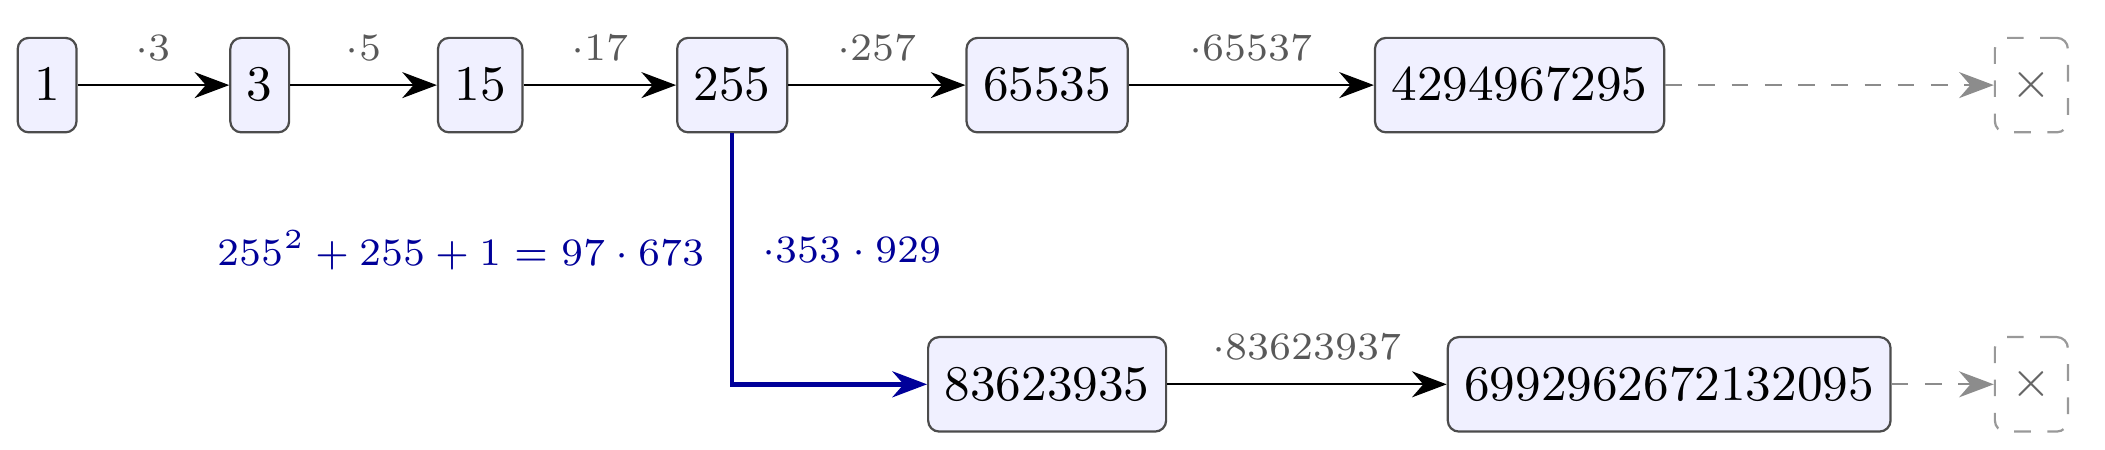
\includegraphics[width=0.84\textwidth]{figures/fig_tree.png}
\caption{The Fermat-type solutions of $n+1=2\varphi(n)$ as the closure
of $1$ under extensions. Horizontal arrows are one-prime extensions
$n_0\mapsto n_0(n_0+2)$, labelled by the prime $n_0+2$. The bent arrow
is the two-prime extension of $255$ by $(353,929)$, coming from the
factorisation $65281=97\cdot673$. Dashed arrows end the two chains:
$4294967297$ and $6992962672132097$ are composite, and neither
$n_0^2+n_0+1$ has a factorisation that yields two primes.}
\label{fig:tree}
\end{figure}

\begin{figure}[t]
\centering
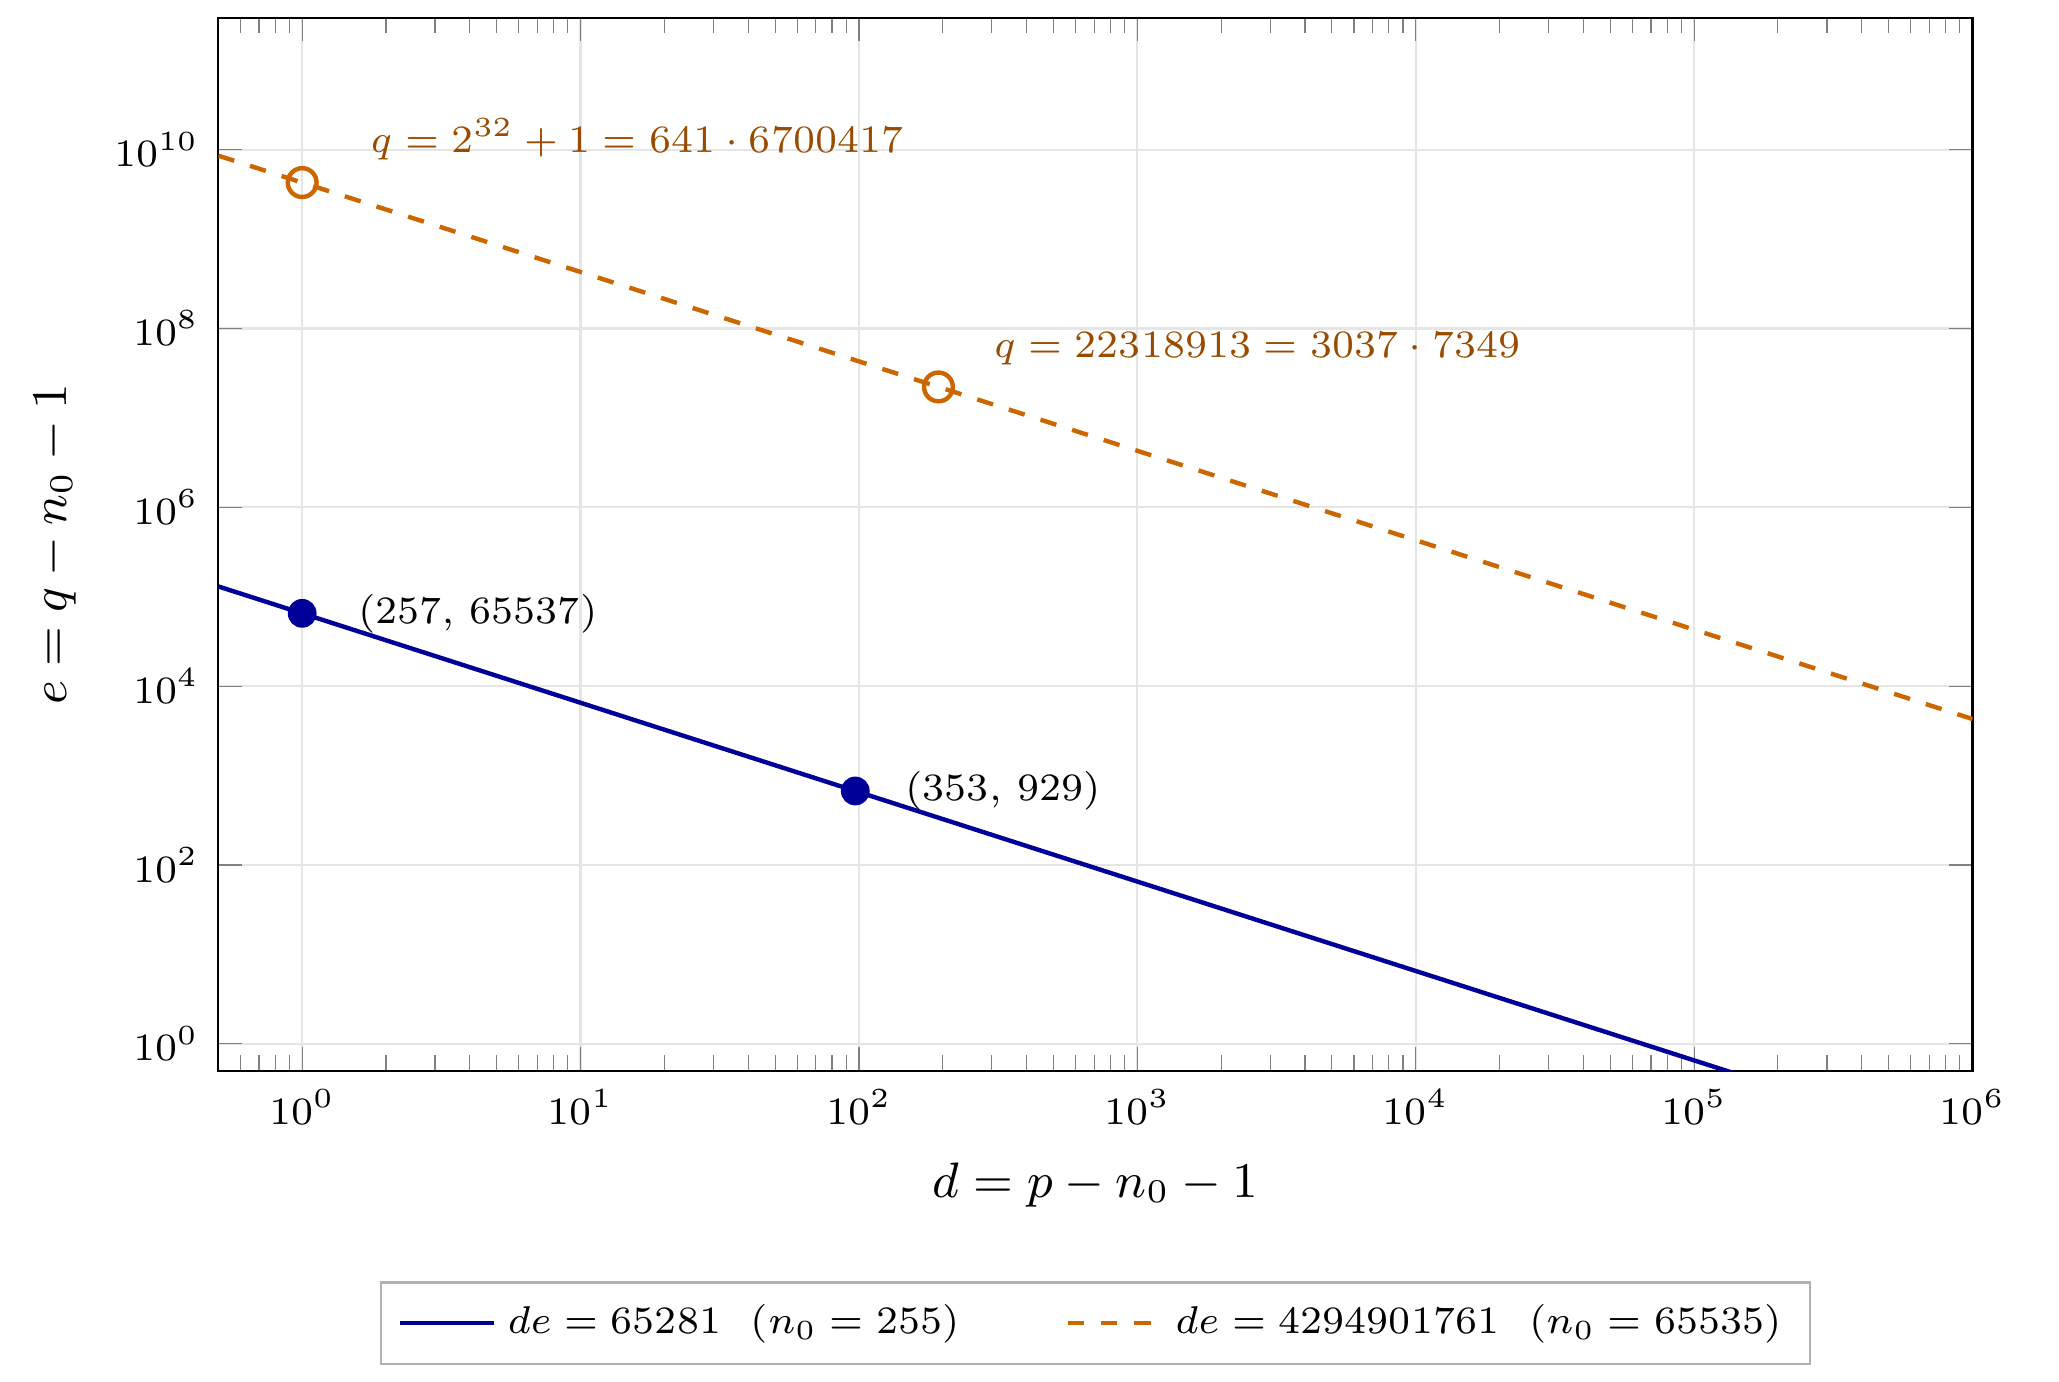
\includegraphics[width=0.82\textwidth]{figures/fig_hyperbola.png}
\caption{The two-prime extensions of $n_0$ are the lattice points
$(d,e)=(p-n_0-1,\,q-n_0-1)$ on $de=n_0^2+n_0+1$ with both $p$ and $q$
prime, shown on logarithmic axes. For $n_0=255$ both lattice points
with $d\le e$ give primes (filled). For $n_0=65535$ both lattice
points give a prime $p$ and a composite $q$ (open).}
\label{fig:hyperbola}
\end{figure}

\begin{remark}\label{rem:three}
For three new primes, $Q=spq$ with $s<p<q$, write $x=s-1$, $y=p-1$, $z=q-1$.
Equation \eqref{eq:ext} becomes
\[
  xyz=n_0\bigl(xy+yz+zx\bigr)+n_0(x+y+z)+n_0+1 ,
\]
and dividing by $n_0xyz$ shows that $1/x+1/y+1/z$ falls short of
$1/n_0$ by $\bigl(n_0(x+y+z)+n_0+1\bigr)/(n_0xyz)$, which is less than
$4/x^2$ because $x<y<z$. Hence $x$, the smallest of the three,
satisfies $3/x>1/n_0-4/x^2$ and $1/x<1/n_0$, that is,
$n_0<x<3n_0+2$. For
fixed $x$ the equation is bilinear in $y$ and $z$:
\[
  \bigl((x-n_0)y-n_0(x+1)\bigr)\bigl((x-n_0)z-n_0(x+1)\bigr)
  =(x-n_0)(n_0x+n_0+1)+n_0^2(x+1)^2 ,
\]
so the pair $(y,z)$ comes from the divisors of an integer of size about
$n_0^2x^2$. For $n_0=4294967295$ there are about $3.8\cdot10^8$
primes $s$ in the range, and $1.3\cdot10^8$ of them pass the
congruence prune: $s\equiv2\pmod3$ as Lemma~\ref{lem:three} requires,
and $s\not\equiv1$ modulo $5$, $17$, $257$ and $65537$. Each of them
leaves an integer of about forty digits to factor. This is the prefix $3,5,17,257,65537$ that
dominates the case $k=8$ in Section~\ref{sec:eight}.
\end{remark}

\subsection{Eight prime factors}\label{sec:eight}
Let $n$ satisfy \eqref{eq:second} with $\omega(n)=8$. Then $n>3$, and
$n$ is odd and squarefree by Lemma~\ref{lem:basic}. If $3\nmid n$, then
$\omega(n)\ge16$ by Theorem~\ref{thm:coprime}; hence $3\mid n$. By
Lemma~\ref{lem:three} the quotient $M$ is either $2$ or at least $5$,
and in the second case $\omega(n)\ge1540$. Hence $n+1=2\varphi(n)$ and
$p_1=3$, and it suffices to run the search with $\varepsilon=+1$ and
$k=8$ over the prefixes that begin with $3$.

The traversal down to depth $5$ takes a few seconds. It yields $10459$
prefixes $(p_1,\dots,p_5)$ with a non-empty interval for $p_6$, and
$10458$ of them begin with $3$. Their intervals have total length
$1.3045\cdot10^{10}$, and most of it belongs to a few prefixes
(Figure~\ref{fig:eight}, left): $8.59\cdot10^9$ to $3,5,17,257,65537$,
that is, to the solution $4294967295$ itself, where $C_5=1$;
$1.23\cdot10^9$ to $3,5,17,257,65543$; and $1.67\cdot10^8$ to
$3,5,17,353,929$, the solution $83623935$, where again $C_5=1$.
Thirty-four prefixes have an interval longer than $10^7$, and $326$
one longer than $10^6$. The intervals contain $228260561$ primes $s$ that
pass the congruence prune, $131788942$ of them for the prefix
$3,5,17,257,65537$. Each pair of a prefix and such a prime $s=p_6$
leaves the two-prime problem of Proposition~\ref{prop:class}, in which
$N$ has between $15$ and $40$ digits.

These problems lie far to the left of those of Figure~\ref{fig:k15}.
For the prefix $3,5,17,257,65537$ and $p_6=s$ one has
$A'=(2^{32}-1)s$ and $B'=2^{31}(s-1)$, so that the modulus is
$c=s-2^{32}$, and $N=2A'B'+c$ is close to $2^{64}s^2$. As $s$ runs
over $[2^{32}+1,\,3\cdot2^{32}-1]$, the ratio $c^3/N$ stays below
$2.1\cdot10^{-10}$, and the number $(N/c^3)^{1/2}$ that governs the
methods of Section~\ref{sec:three} grows from $7\cdot10^4$ at the
upper end to $4\cdot10^{16}$ at the first admissible prime,
$s=4294967357$, where $c=61$. We therefore combine the sum route with
trial division and with a complete factorisation, as follows.

Fix a prefix and an admissible prime $s$, define $A'$, $B'$, $c$, $N$
as in Section~\ref{sec:three}, and let $t=cp-2B'$ be the divisor of
Proposition~\ref{prop:class}. Since $p\ge s+2$, it satisfies
$t\ge t_0=c(s+2)-2B'$, and we choose a split point $t_d$ with
$t_0\le t_d$.
\begin{enumerate}[label=\textup{(\roman*)}, leftmargin=*]
\item The divisors with $t<t_d$ are found by running $p$ over the
  integers with $t_0\le cp-2B'<t_d$ and testing whether $t$ divides
  $A'p+\varepsilon$, as in Proposition~\ref{prop:last}. Since
  $c(A'p+\varepsilon)=A't+N$ and $\gcd(t,c)=1$ by
  Proposition~\ref{prop:class}, this is the same as testing whether $t$
  divides $N$, and the program does that when $A'p$ is too large for
  $128$-bit arithmetic.
\item For the divisors with $t_d\le t\le\sqrt N$ we use the sum
  $\sigma=p+q$ and the product $\pi=pq$. By \eqref{eq:hyperbola},
  \begin{equation}\label{eq:sigma}
    c\,\pi=2B'\sigma-2B'+\varepsilon,\qquad
    (q-p)^2=\sigma^2-4\pi ,
  \end{equation}
  so $\sigma$ lies in the class of $(2B'-\varepsilon)(2B')^{-1}$ modulo
  $c$, and $t+N/t=c\sigma-4B'$. As $x+N/x$ decreases on
  $(0,\sqrt N\,]$, the sum runs over its class in the range
  $2\sqrt N+4B'\le c\sigma\le t_d+N/t_d+4B'$, and each value is
  tested by asking whether $\sigma^2-4\pi$ is a perfect square. This
  is the route of Section~\ref{sec:sum}, written in terms of $p$ and
  $q$ instead of $u$ and $v$: the two sums differ by the constant
  $(2r+4B')/c$.
\item Both loops are sieved by congruences. Let $p<q$ be integers
  with $A'pq+1=2B'(p-1)(q-1)$. No $p_i$ divides $p-1$ or $q-1$, since
  it would then divide $1$. If moreover $p$ and $q$ have no prime
  factor up to $61$, which holds for primes larger than $s$ because
  every admissible $s$ exceeds $61$, then modulo every prime $\ell\le61$
  they avoid the residue $0$, and also the residue $1$ when $\ell$ is
  one of the $p_i$; in particular they are odd and congruent to $2$
  modulo $3$. Call these residues excluded. Since
  $X^2-\sigma X+\pi=(X-p)(X-q)$, the roots of this polynomial modulo a
  prime $\ell$ are $p$ and $q$ modulo $\ell$. The sieve discards only
  values of $\sigma$ that are odd, or not congruent to $1$ modulo $3$,
  or for which $\sigma^2-4\pi$ is not a square modulo one of $2^8$,
  $3^2$, $5^2$ and $7^2$, or for which, for some prime $\ell\le43$,
  the polynomial has no root modulo $\ell$ or a root at an excluded
  residue; and in the trial division it discards only values of $p$
  at an excluded residue modulo some prime $\ell\le61$. Every other
  value is tested exactly. So the sieve keeps every value that comes
  from integers $p$ and $q$ without prime factors up to $61$, and in
  particular every value that comes from primes.
\item If the estimated work of (i) and (ii) exceeds four milliseconds,
  the time we allow for factoring $N$, then $N$ is factored completely with
  PARI/GP \cite{PARI}, every prime factor is proved
  prime,\footnote{With the option \texttt{factor\_proven} set, PARI/GP
  certifies every prime factor it returns. A factor below $2^{64}$ is
  certified by its Baillie--PSW test, which no composite number below
  $2^{64}$ passes; the PARI/GP documentation records that this was
  checked against the table of base-$2$ pseudoprimes below $2^{64}$ of
  Feitsma and Galway \cite{FG}. A larger factor is certified by the
  $n-1$ method \cite{BLS75} when enough of $n-1$ is known, and
  otherwise by the test of Adleman, Pomerance and Rumely
  \cite{APR83} in the form of Cohen and Lenstra \cite{CL84}.} and all
  divisors $t$ of $N$ with $t_0\le t\le\sqrt N$ in the class of
  Proposition~\ref{prop:class} are listed.
\end{enumerate}
Since $c$ is odd and prime to $3$, the admissible values of $\sigma$
form one class modulo $6c$. The work of (i) and (ii) is therefore about
$(t_d-t_0)/c$ values of $p$ and $(t_d+N/t_d-2\sqrt N)/(6c^2)$ values of
$\sigma$, and $t_d$ is chosen to minimise it (Figure~\ref{fig:routes}),
with the two kinds of steps weighted by their measured costs. With equal weights the minimum
lies near $t_d=(N/6c)^{1/2}$ and amounts to about $2(N/6c^3)^{1/2}$
steps, as in Section~\ref{sec:sum}. By the argument of that section,
(i) and (ii) together find every divisor $t\ge t_0$ of $N$ in the class
up to $\sqrt N$, and so does (iv); the sieve (iii) loses none that
comes from integers $p$ and $q$ without prime factors up to $61$. Where
$\sigma$ and $\pi$ are too large for $128$-bit arithmetic, (ii) is
carried out in multiprecision arithmetic. Now let $n$ be a solution with
$p_1=3$ and $k=8$. By Theorem~\ref{thm:complete} its first five primes
form one of the prefixes and $p_6$ is one of the admissible primes $s$
of its interval, and by Proposition~\ref{prop:class} its last two
primes give a divisor $t\ge t_0$ in the class. Hence $n$ is found.
Every completion $s<p<q$ in integers that is found is checked against
$A'pq+1=2B'(p-1)(q-1)$ exactly, and $p$ and $q$ are tested for
primality.

The computation examined all $228260561$ pairs; in $1967265$ of them
$N$ was factored, with up to $39$ digits (Appendix~\ref{sec:checks8}
gives the size of the run). It found $21$ completions $s<p<q$ in
integers and no solution. Sixteen of the completions lie under the prefix
$3,5,17,353,929$ with $s=83623937$, where
$3\cdot5\cdot17\cdot353\cdot929\cdot s$ is the solution
$n_0=6992962672132095$. They are the pairs $p=n_0+1+d$, $q=n_0+1+e$ of
Theorem~\ref{thm:ext}(ii), one for each factorisation
$n_0^2+n_0+1=de$ with $d<e$, and by Table~\ref{tab:ext} none of them
consists of two primes. In each of the other five, listed in
Table~\ref{tab:eight}, $p$ or $q$ is divisible by one of
$p_1,\dots,p_5$. So \eqref{eq:second} has no solution with eight prime
factors, and
together with Section~\ref{sec:seven} this proves
Theorem~\ref{thm:eight}.

\begin{figure}[t]
\centering
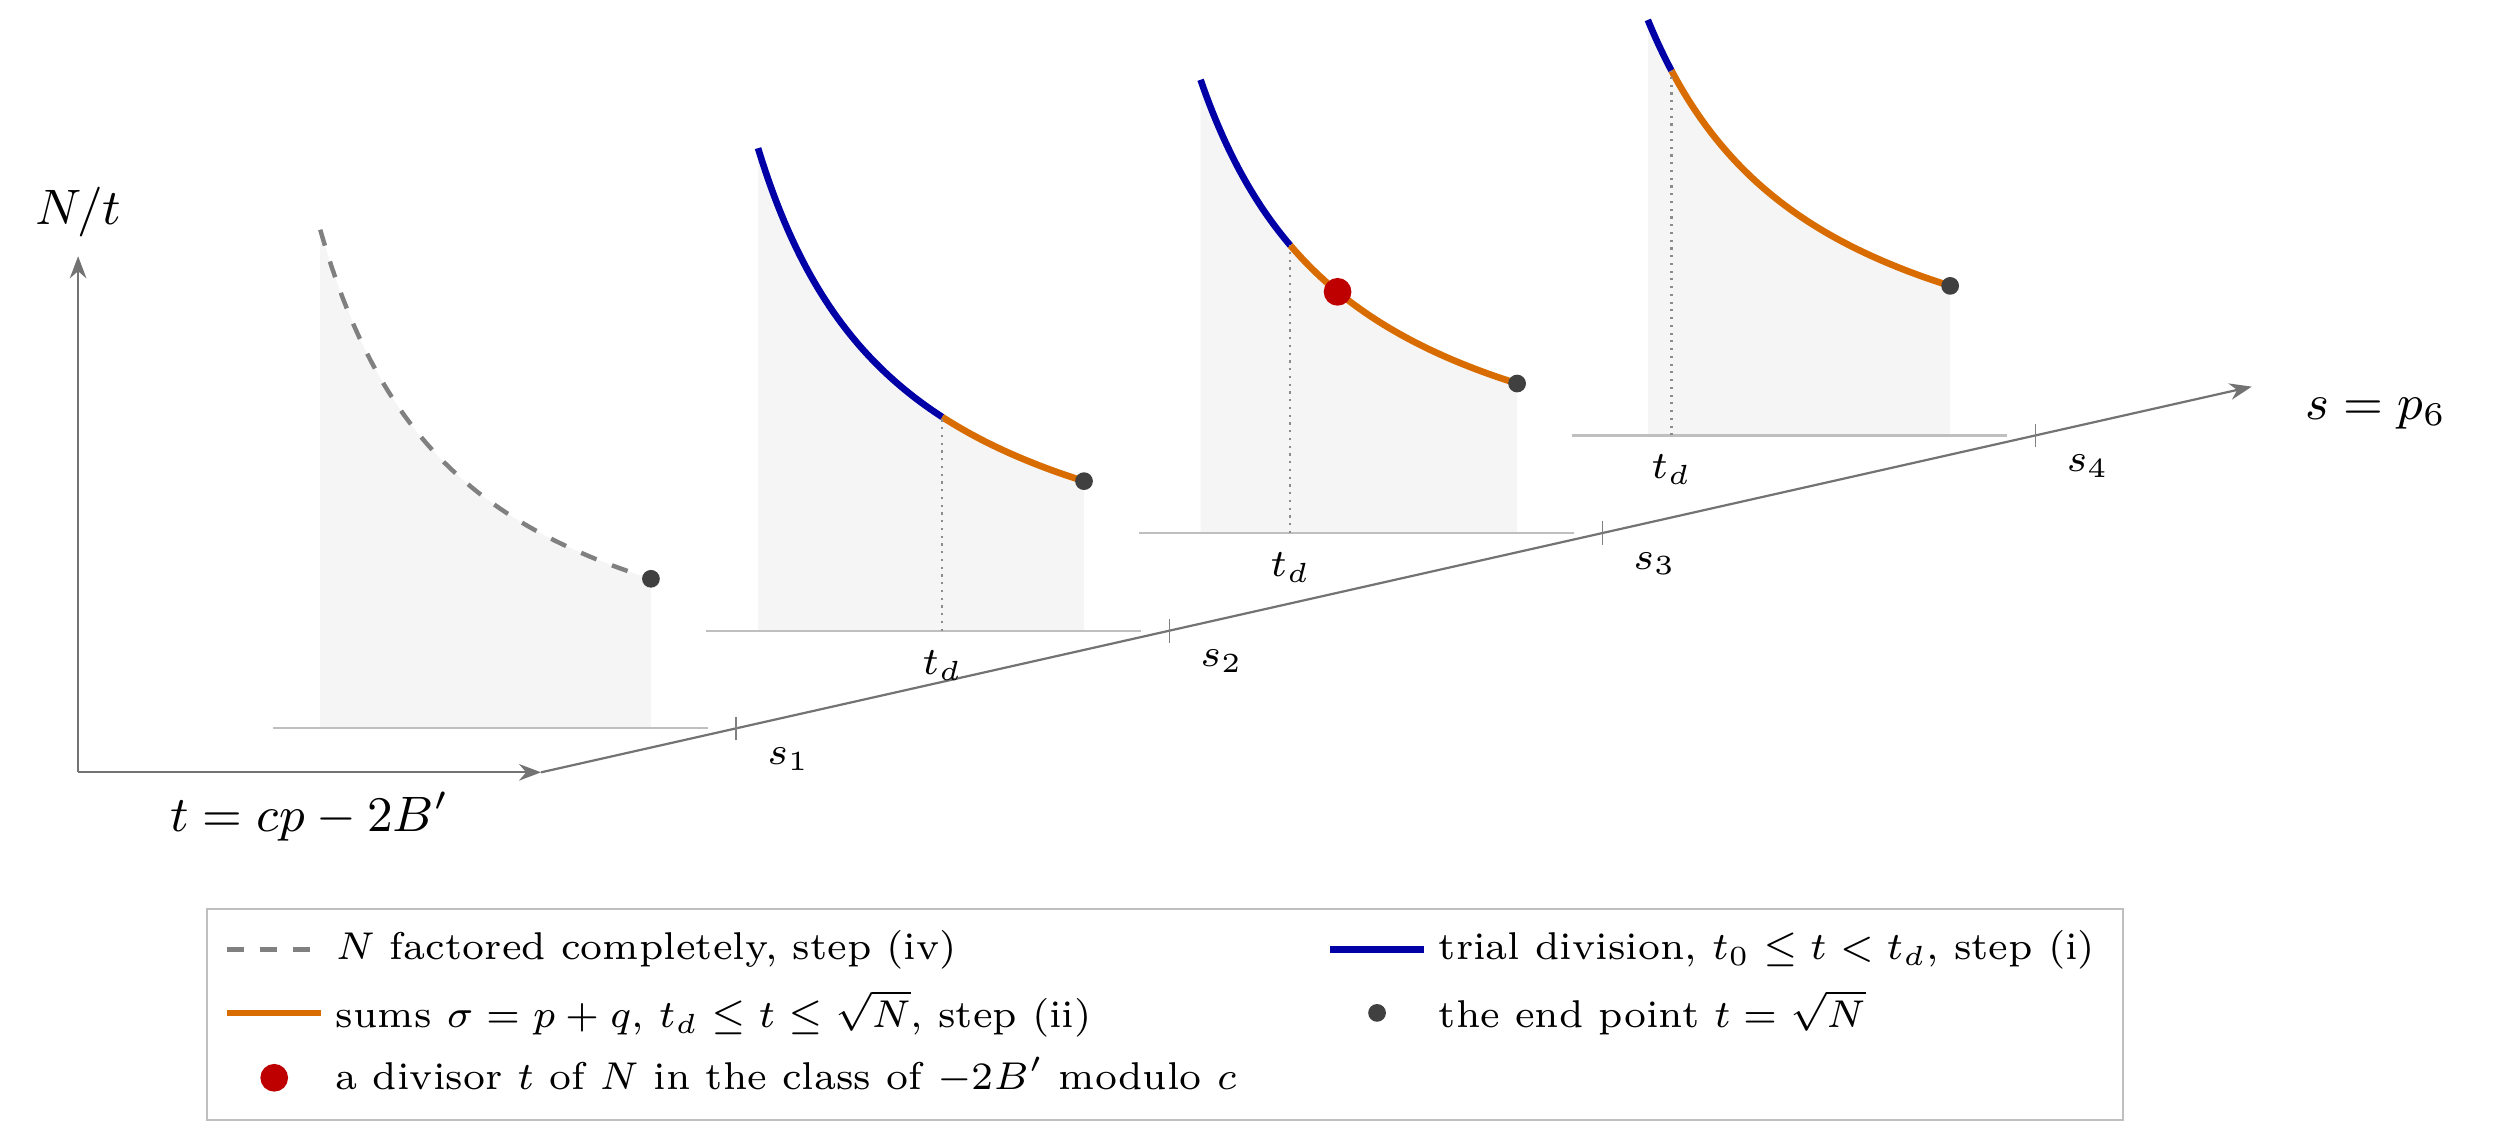
\includegraphics[width=\textwidth]{figures/fig_routes.png}
\caption{Steps (i), (ii) and (iv) for four admissible values
$s_1<s_2<s_3<s_4$ of $p_6$, not to scale. The divisors $t=cp-2B'$ of
$N$ with $t_0\le t\le\sqrt N$ lie on the branch $t\mapsto N/t$.
Trial division covers $t<t_d$ and the sums cover $t_d\le t\le\sqrt N$.
The split point $t_d$ is chosen for each $s$ to minimise the work, and
where both routes would be slow, as for $s_1$, the integer $N$ is
factored completely.}
\label{fig:routes}
\end{figure}

\begin{table}[ht]
\centering
\caption{The completions $s<p<q$ in integers of the case $k=8$ other
than the sixteen two-prime extensions of $6992962672132095$, with the
factorisations of $p$ and $q$.}
\label{tab:eight}
\smallskip
\footnotesize
\begin{tabular}{@{}lll@{}}
\toprule
$s=p_6$ & $p$ & $q$ \\
\midrule
\multicolumn{3}{@{}l}{prefix $3,5,17,257,65537$} \\
$4294967459$ & $17\cdot43\cdot673\cdot230521189693$ & $5\cdot409642859\cdot26363459459$ \\
$4294967969$ & $27419312914203719$ & $5\cdot19\cdot5011\cdot7699\cdot21393991009$ \\
$4596195557$ & $65533391633$ & $17\cdot20923232569978145771052877$ \\
\multicolumn{3}{@{}l}{prefix $3,5,17,353,929$} \\
$83625827$ & $3^2\cdot5^3\cdot13\cdot252862031$ & $3\cdot5\cdot7\cdot13\cdot113\cdot794656817253868193$ \\
$83760029$ & $3\cdot5\cdot3431155289$ & $3\cdot87389293\cdot45294677621$ \\
\bottomrule
\end{tabular}
\end{table}

\begin{figure}[t]
\centering
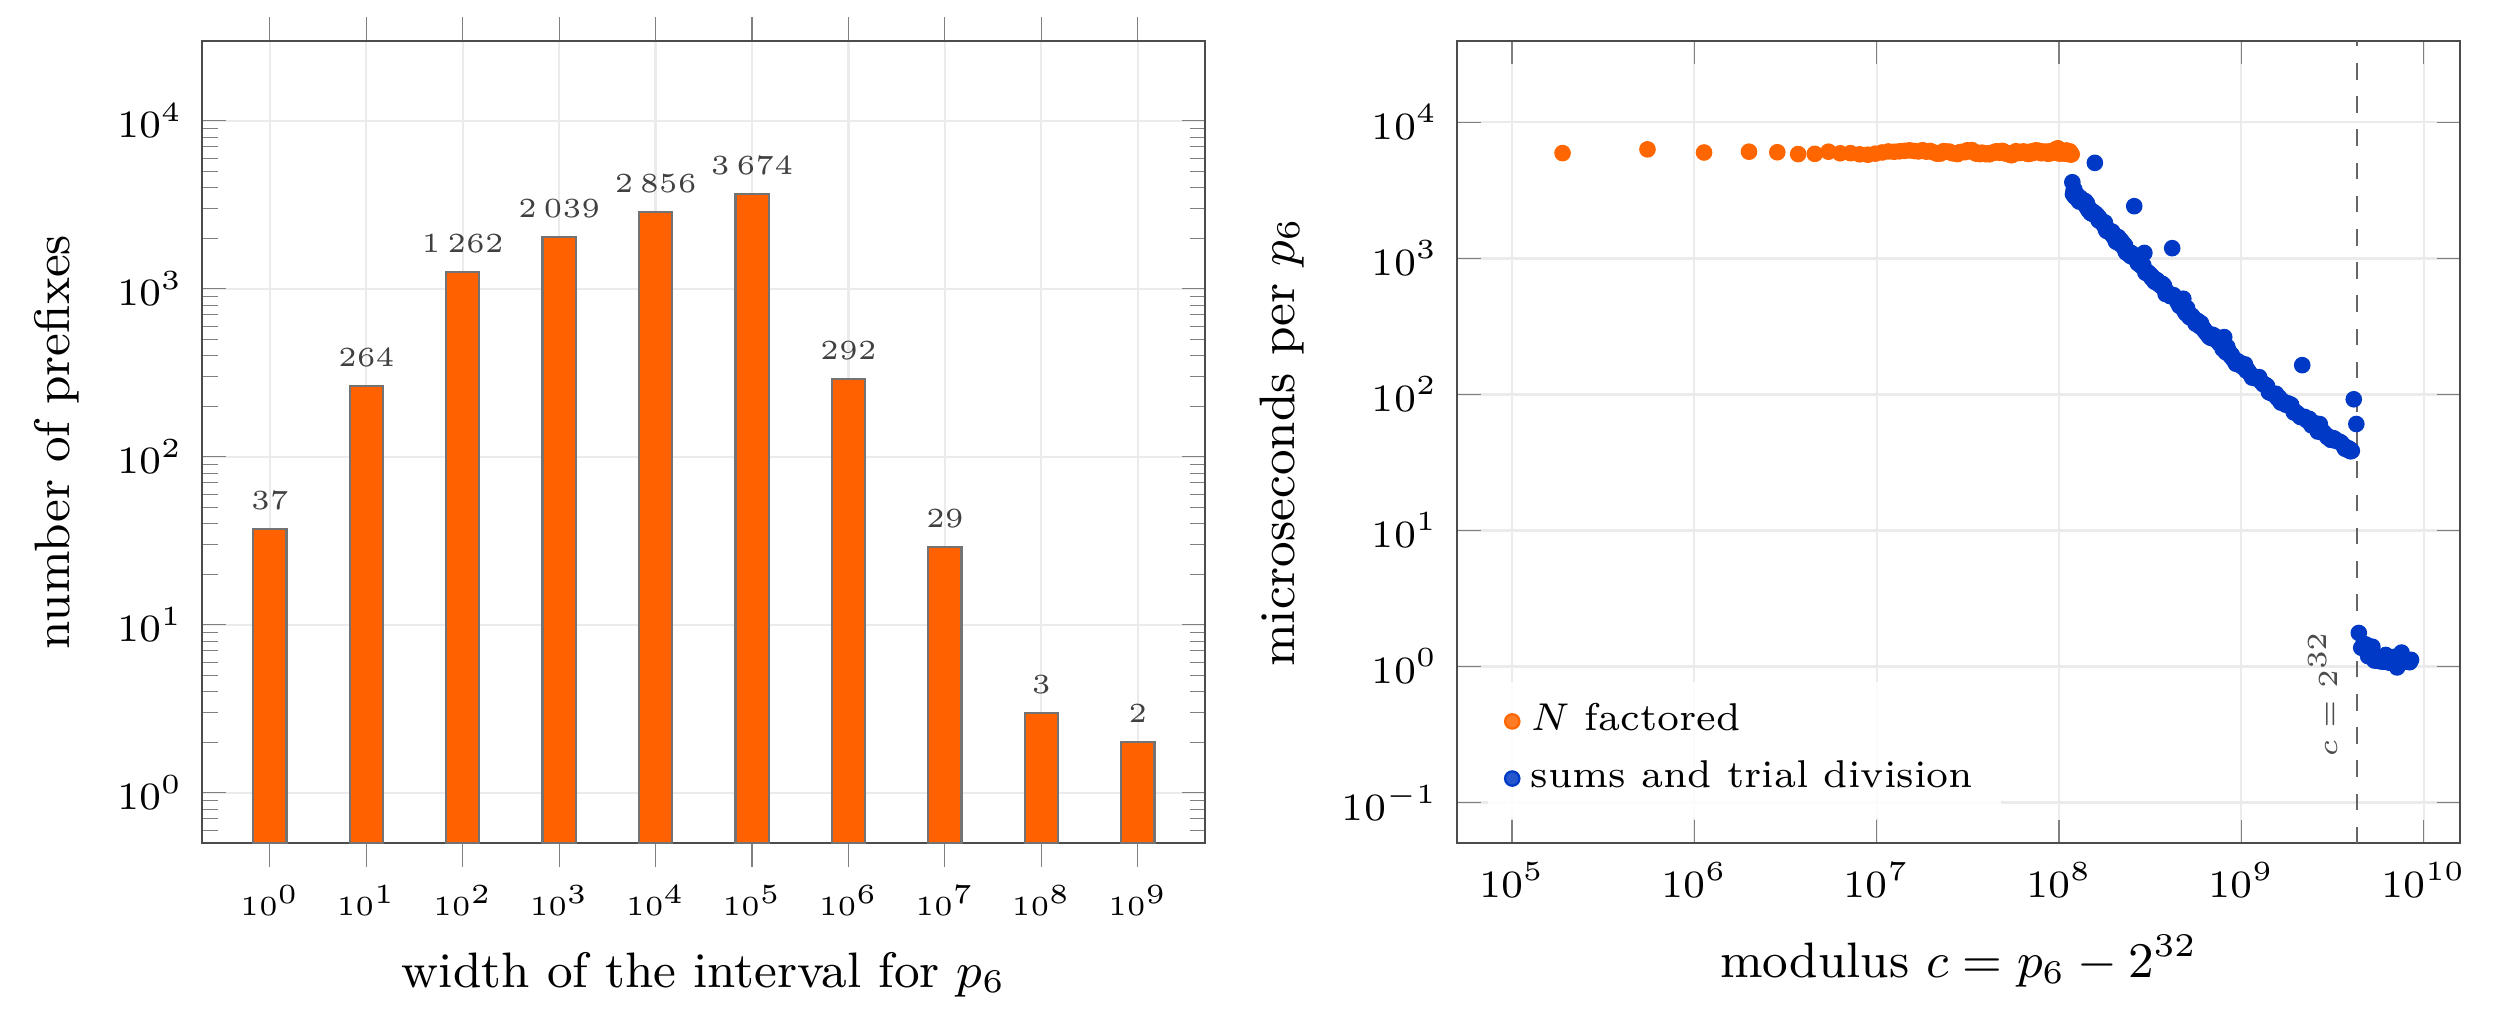
\includegraphics[width=\textwidth]{figures/fig_eight.png}
\caption{The case $k=8$ of the companion equation. Left: the
$10458$ prefixes $(3,p_2,\dots,p_5)$ by the width of the interval for
$p_6$, on logarithmic axes; the two in the last bar end in $65537$ and
$65543$. Right: processor time per admissible $p_6$ under the prefix
$3,5,17,257,65537$, one point for each piece of the run, against the
modulus $c=p_6-2^{32}$. For $c$ below about $10^8$ the integer $N$ is
factored, and each $p_6$ costs about six milliseconds in all; above that the sums and the
trial division are faster, and their cost falls as $c$ grows. Beyond
$c=2^{32}$, that is for $p_6>2^{33}$, the condition $p>p_6$ leaves only
a short range of divisors.}
\label{fig:eight}
\end{figure}

%%==================================================================
\section{Checks on the computations}\label{sec:checks}
%%==================================================================

A search that finds nothing proves something only if it would have
found what it looks for. Every search of this paper was therefore
carried out by at least two programs written independently, and every
count reported here is the same for all of them. For
Theorems~\ref{thm:first} and~\ref{thm:coprime} one of the two programs
never factors an integer, so that its negative answers depend on no
primality proof. The programs were also run on equations that do have
solutions: on the equation $2^k(n-1)=(2^k+h)\varphi(n)$, whose $56$
solutions with $k=4$ and $k=5$ in the ranges of
Appendix~\ref{app:known} they all return, and on \eqref{eq:second},
where they return every known solution with at most six prime factors
at the right depth and nothing else. The divisor routines of
Section~\ref{sec:three} were compared with complete factorisations and
tested on planted divisors, and the program of Section~\ref{sec:eight}
was tested in the same ways and partly run twice.
Appendix~\ref{app:checks} gives the details.

%%==================================================================
\section{The next cases}\label{sec:walls}
%%==================================================================

The methods of Section~\ref{sec:three} settle the case $k=15$ in a
quarter of an hour on a single processor, and the case of eight primes
of the companion equation in $6.9$ hours. This section explains why
they do not reach the next cases, and which properties of the primes
any further progress has to use.

\subsection{Lehmer's equation with sixteen primes}\label{sec:sixteen}
By Theorem~\ref{thm:size}(i) a solution with sixteen prime factors
would lie below $2^{512}$. For $k=16$ the traversal down to depth $12$ is again a matter of
seconds. It produces $90092$ prefixes with four primes still to
choose, and their intervals for $p_{13}$ have total length
$1.6\cdot10^9$ (Figure~\ref{fig:walls}). They contain
$1.2\cdot10^8$ primes, of which $5.4\cdot10^7$ pass the congruence
prune. The widest interval, of length $1.6\cdot10^8$, belongs once
more to the prefix ending in $25867$. Each admissible $p_{13}$ now
leaves three primes to choose, and every admissible $p_{14}$ then
leaves a two-prime problem of the kind solved in
Section~\ref{sec:three}. Near the lower end of a long interval the shortfall
$C_{13}/A_{13}$ after $p_{13}$ is tiny, so the interval for $p_{14}$
is very long. If $T-1$ is the shortfall after twelve primes, and $x_0$
is about $1/(T-1)$, a choice $p_{13}=x_0+d$ leaves a shortfall of about
$(T-1)^2d$ and hence an interval of length about
$2/\bigl((T-1)^2d\bigr)$ for $p_{14}$. Summing over the admissible
primes $p_{13}$, and counting the primes $p_{14}$ with density
$1/\log x$ and the share of them that passes the prune, gives to first
order some $4\cdot10^{14}$ pairs of primes $(p_{13},p_{14})$, of which
about $9\cdot10^{13}$ are admissible, two thirds of these from the
single prefix ending in $25867$, where $T-1=1.8\cdot10^{-8}$. The integers $N$ of the resulting two-prime problems are as large as
$10^{86}$, and about $10^{77}$ on average. At the average speed of the sum route for
$k=15$, $24$ microseconds per problem, the admissible pairs alone
would take $2\cdot10^9$ processor seconds. The problems with a small
modulus add to this. Close to the lower end of each interval for $p_{14}$
the modulus $c$ is small: about eleven per cent of the problems have
$c^3<N$, where the work grows like $(N/c^3)^{1/2}$, some $10^9$ have
$c^3/N<10^{-12}$, and for the smallest $c$ the integer $N$ would have
to be factored. With these the total is of the order of $10^{10}$
processor seconds, some three centuries. The case $k=16$ is therefore
far beyond a single machine. It needs either a computation of that size or a
method that treats a whole range of $p_{13}$ at once.

\begin{figure}[t]
\centering
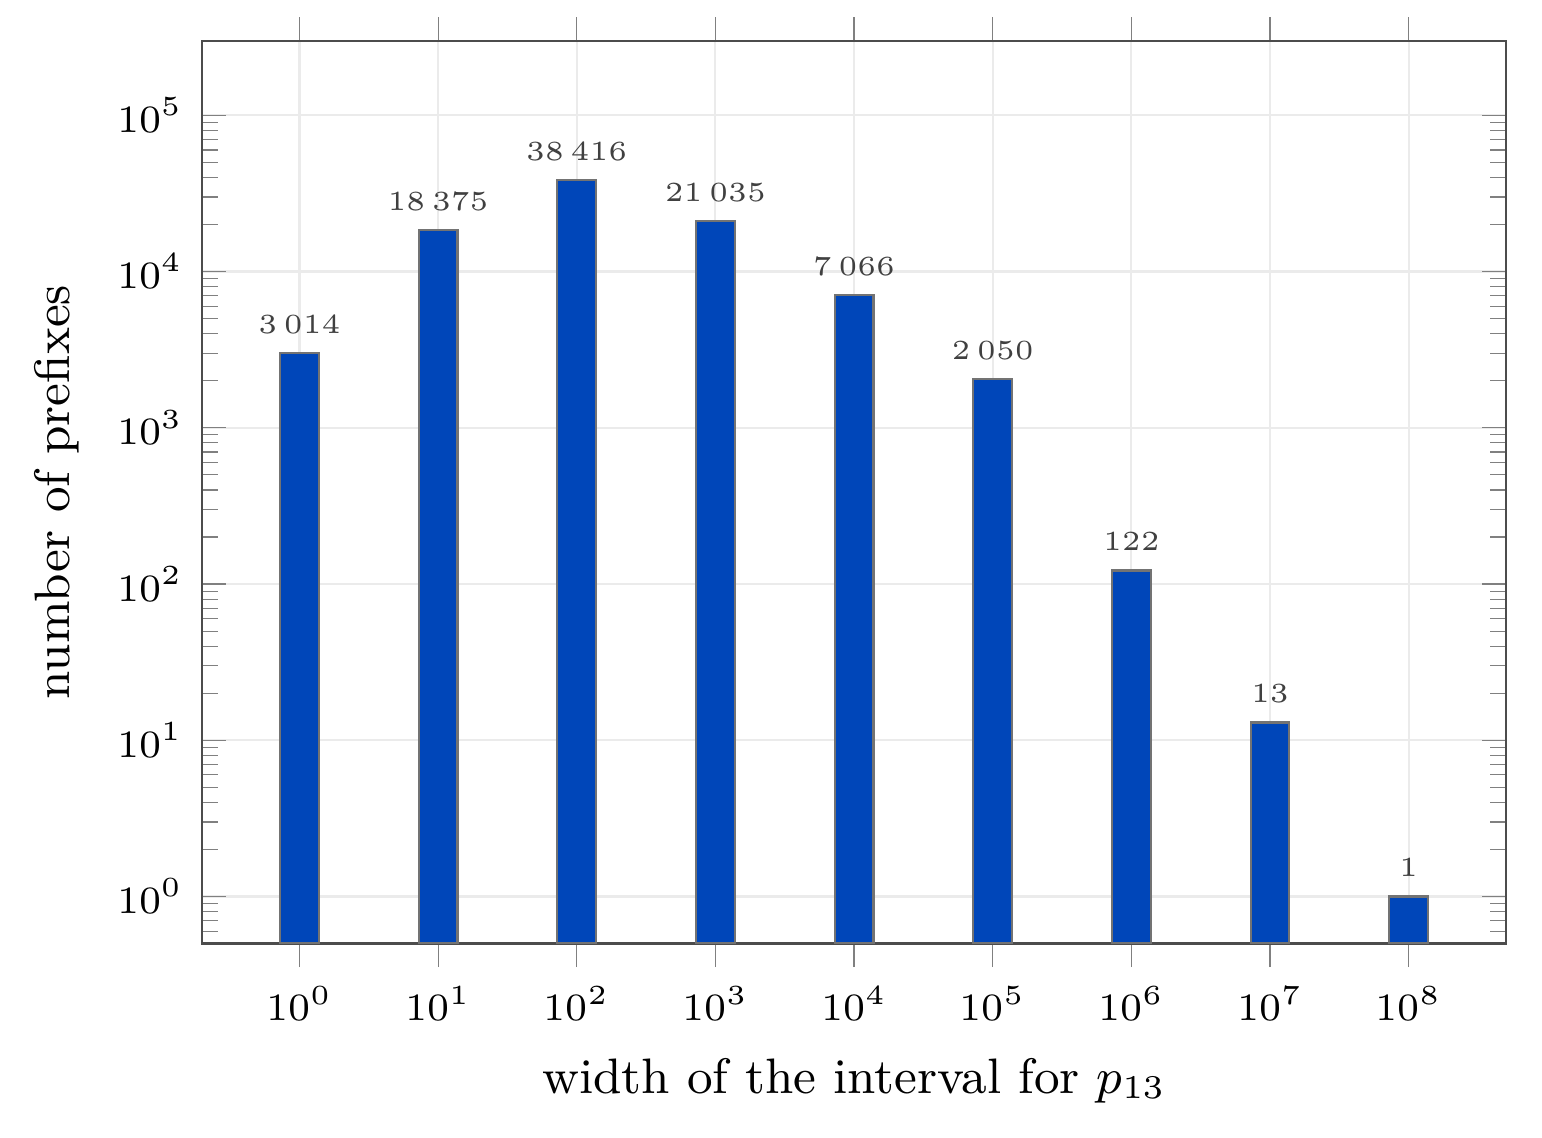
\includegraphics[width=0.62\textwidth]{figures/fig_walls.png}
\caption{The $90092$ prefixes of twelve primes for $n-1=2\varphi(n)$
with $k=16$, by the width of the interval for $p_{13}$, on logarithmic
axes. The single prefix in the last bar ends in $25867$.}
\label{fig:walls}
\end{figure}

\subsection{The companion equation with nine primes}
For \eqref{eq:second}, Theorems~\ref{thm:eight} and \ref{thm:coprime}
leave open the solutions with $3\mid n$ and $\omega(n)\ge9$, and those
with $3\nmid n$ and $\omega(n)\ge16$. In the first family the Fermat
primes make the next case far harder than the last. Under the prefix
$3,5,17,257,65537$ every admissible $p_6=s$ now leaves three primes to
choose, and the shortfall after six primes is $c/A'$ with $c=s-2^{32}$
and $A'=(2^{32}-1)s$, so that the interval for $p_7$ runs from about
$A'/c$ to $3A'/c$. Near the lower end of the interval for $p_6$ this
is an interval of length about $10^{18}$. Counting the admissible
primes $s$ exactly up to $s=2^{32}+10^7$ and estimating the rest, and
counting the primes $p_7$ with density $1/\log x$ and the share of
them that passes the prune, gives some $1.6\cdot10^{17}$ two-prime
problems from this one prefix, each with an integer $N$ of between
$60$ and $75$ digits. At a microsecond per problem this would take five
thousand years of processor time, so the case $k=9$ with $3\mid n$ is
out of reach of these methods.

\subsection{Pseudo-solutions}
Apart from the primality tests, the traversal of Section~\ref{sec:search}
uses only the following properties of the tuple $(p_1,\dots,p_k)$:
its entries are odd and increasing, they satisfy
\begin{equation}\label{eq:product}
  x_1x_2\cdots x_k+\varepsilon=2(x_1-1)(x_2-1)\cdots(x_k-1),
\end{equation}
and $\gcd(x_i,x_j-1)=1$ for all $i$ and $j$. Indeed the proofs of
Propositions~\ref{prop:below2}, \ref{prop:bounds} and~\ref{prop:last}
use nothing else once $\varphi(n)$ is replaced by
$\prod_i(x_i-1)$. We call a tuple with these properties a
\emph{pseudo-solution} if not all its entries are prime.

\begin{proposition}\label{prop:pseudo}
Let $n_0=p_1\cdots p_m$ be a Fermat-type solution with $m\ge2$ prime
factors $p_1<\dots<p_m$. Then $(p_1,\dots,p_m,n_0)$ is a
pseudo-solution of \eqref{eq:product} with $\varepsilon=-1$.
\end{proposition}

\begin{proof}
The entries are odd and increasing, and $n_0$ is composite. Since $n_0$
is squarefree, $\prod_i(p_i-1)=\varphi(n_0)=(n_0+1)/2$, and so
\[
  p_1\cdots p_m\,n_0-1=n_0^2-1=2\cdot\frac{n_0+1}{2}\cdot(n_0-1)
  =2\prod_{i\le m}(p_i-1)\cdot(n_0-1).
\]
Lemma~\ref{lem:basic}(ii), applied to $n_0$ with $\varepsilon=+1$,
gives $p_i\nmid p_j-1$ for all $i,j\le m$; hence $\gcd(p_i,p_j-1)=1$
and, as $n_0$ is the product of the $p_i$, $\gcd(n_0,p_j-1)=1$.
Finally $\gcd(n_0,n_0-1)=1$, and so $\gcd(p_i,n_0-1)=1$ because
$p_i\mid n_0$.
\end{proof}

The six Fermat-type solutions in \eqref{eq:known} with at least two
prime factors give pseudo-solutions with $k=3,4,5,6,6,7$ entries, the
smallest being $(3,5,15)$, for which $3\cdot5\cdot15-1=224=2\cdot2\cdot4\cdot14$.
Run with $\varepsilon=-1$ and $p_{\min}=3$, the search of
Section~\ref{sec:search} reaches each of them as a lattice point on
the hyperbola \eqref{eq:hyperbola} and rejects it only because its last
entry is composite. In the proof of Theorem~\ref{thm:first} they never
arise, because Lemma~\ref{lem:three} excludes $3\mid n$, and that
lemma rests on primality once more: its proof needs that a prime other
than $3$ is prime to $3$, and the entry $15$ is not.
Consequently no argument that uses only \eqref{eq:product}, the order
of the entries and the conditions $\gcd(x_i,x_j-1)=1$ can exclude
solutions of $n-1=2\varphi(n)$ with $k$ prime factors for any $k$ with
$3\le k\le7$; the primality of the entries has to enter the argument.

\subsection{Pseudo-solutions prime to \texorpdfstring{$3$}{3}}
The conditions $\gcd(x_i,x_j-1)=1$ are consequences of
\eqref{eq:product}, since a common divisor of $x_1\cdots x_k$ and
$\prod_j(x_j-1)$ divides $\varepsilon$. What separates the
pseudo-solutions of Proposition~\ref{prop:pseudo} from solutions of
Lehmer's equation is the prime $3$.

\begin{lemma}\label{lem:parity}
Let $x_1,\dots,x_k$ be integers with
$x_1\cdots x_k+\varepsilon=M\prod_i(x_i-1)$, where
$\varepsilon=\pm1$, and suppose that exactly $\nu\ge1$ of them are
divisible by $3$. Then $\varepsilon\equiv(-1)^{\nu}M\pmod3$. In particular
a solution of \eqref{eq:product} has $\nu$ even if $\varepsilon=-1$, and
$\nu=0$ or $\nu$ odd if $\varepsilon=+1$.
\end{lemma}

\begin{proof}
A common divisor of $x_i$ and $x_j-1$ divides both $x_1\cdots x_k$ and
$M\prod_i(x_i-1)$, hence $\varepsilon$, so $\gcd(x_i,x_j-1)=1$ for all
$i$ and $j$. Let $3\mid x_i$. Then no $x_j$ is congruent to $1$ modulo
$3$. Hence $x_j-1\equiv-1\pmod3$ if $3\mid x_j$
and $x_j-1\equiv1\pmod3$ otherwise, and the equation modulo $3$ reads
$\varepsilon\equiv(-1)^{\nu}M$. For $M=2$ this is
$\varepsilon\equiv(-1)^{\nu+1}$.
\end{proof}

For $\nu=1$ this is the congruence of Lemma~\ref{lem:three}. The
pseudo-solutions that Proposition~\ref{prop:pseudo} builds from the
solutions in \eqref{eq:known} have $\nu=2$, since $3$ divides both
$p_1$ and $n_0$, whereas the prime factors of $n$ give
$\nu\le1$. The fact that $3$ divides at most one prime factor therefore
removes all of them, and by Lemma~\ref{lem:parity} a pseudo-solution
of Lehmer's equation with pairwise coprime entries has $\nu=0$. We call
a pseudo-solution with $\nu=0$ \emph{prime to $3$}.

\begin{theorem}\label{thm:pseudo3}
Let $\varepsilon=\pm1$.
\begin{enumerate}
\item[(i)] No pseudo-solution of \eqref{eq:product} with $k\le13$ is
prime to $3$.
\item[(ii)] For $k\le15$ no pseudo-solution of \eqref{eq:product} prime
to $3$ has $x_1,\dots,x_{k-3}$ prime.
\end{enumerate}
\end{theorem}

\begin{proof}
The proofs of Propositions~\ref{prop:below2}, \ref{prop:bounds}
and~\ref{prop:last} use only \eqref{eq:product} and the order of the
entries, so the traversal of Section~\ref{sec:search} applies to odd
integers prime to $3$, with the congruence prune replaced by
$x\not\equiv0$ modulo the odd primes of $B_j$ and $x\not\equiv1$ modulo
the primes of $A_j$. For (i) the tree is traversed with integer entries
down to depth $k-3$; for $k=12$ it has $489$ nodes at that depth, below
which lie $55423$ admissible values of $x_{k-2}$. For (ii) the
traversal with prime entries is run to depth $k-3$. For $k\le12$ in
(i), and for every $k$ in (ii), every admissible odd $x_{k-2}$ prime to
$3$ in the interval is followed by the sum route of
Section~\ref{sec:sum}, which does not use primality. For $k=15$ in
(ii) these are $1.43\cdot10^8$ values of $x_{k-2}$ for each sign,
treated in about four minutes per sign; for eight of them per sign the
route would be long, and there $2AB+\varepsilon C$ is factored
completely, with every prime factor proved prime. No completion occurs.

For $k=13$ in (i) the tree has $86459$ nodes at depth $10$, the same
for both signs. Their intervals for $x_{11}$ have total length
$1.07\cdot10^{11}$ and contain $1.64\cdot10^{10}$ admissible values;
the longest, of length $1.9\cdot10^{10}$, belongs to the prefix
$5,7,13,17,19,23,25,37,119,147089$. These values are treated by the
program of Section~\ref{sec:eight}, with the conditions on primes
replaced by those of the integer prune: modulo $2$, modulo $3$ and
modulo the odd primes of $B_{10}$ the residue $0$ is excluded, and
modulo the primes of $A_{10}$ the residue $1$. Every completion in odd
integers prime to $3$ avoids these residues, because
$\gcd(x_i,x_j-1)=1$, so the sieve loses none of them. For $73106$
values, near the lower ends of the longest intervals, the integer
$2AB+\varepsilon C$, of up to $54$ digits, is factored completely
instead, with every prime factor proved prime. The program chooses
these values from its estimate of the running time, which depends on
$\varepsilon$ only through the term $\varepsilon C$, negligible beside
$2AB$; it chooses the same $73106$ values for both signs. The run took
about $15$ hours of processor time per sign, $2.5$ of them in PARI/GP,
and found no completion in odd integers prime to $3$ for either sign.
A second program factors each integer $2AB+\varepsilon C$ completely
with PARI/GP \cite{PARI}, proves every prime factor prime, and runs through all its
divisors in the class of Proposition~\ref{prop:class}. It traverses
the integer tree independently, with its own bounds, and repeats (i)
for $k\le12$; it repeats (ii) for $k\le14$, including all $67626$ values of $x_{11}$
at $k=14$, with the same result. The case $k=13$ of (i) rests on the
program of Section~\ref{sec:eight} and its checks in
Appendix~\ref{sec:checks8}. Allowed to use the entry $3$, the
second program finds $1$, $1$, $2$, $8$ and $47$ solutions of
\eqref{eq:product} in odd integers with $\varepsilon=-1$ for
$k=3,\dots,7$, all with $\nu\in\{2,4\}$, and $1$, $1$, $2$, $4$ and $18$
with $\varepsilon=+1$, all with $\nu$ odd; the first program, run on
prime prefixes, finds exactly those whose first $k-3$ entries are
prime.
\end{proof}

Theorem~\ref{thm:pseudo3} says that for $k\le13$ the search behind
Theorem~\ref{thm:first}, which solves \eqref{eq:product} with
$\varepsilon=-1$ and $x_1\ge5$, needs no primality beyond the fact
that $3$ divides at most one prime factor, and that for $k\le15$ it
needs the primality of the first $k-3$ factors only.

Tuples of this kind have also been studied by Molnar and Singh
\cite{MS25}, who call integers $x_1,\dots,x_r\ge2$, not necessarily
distinct, with $\prod_i(x_i-1)$ dividing $\prod_ix_i-1$ a spoof Lehmer
factorisation. They give an algorithm that finds all of them with a
given number of entries, and list the $31$ with odd entries and at most
six of them \cite[Theorem~7 and Table~1]{MS25}. Twelve of the $31$
have distinct entries, and all twelve have quotient $2$. They are
exactly the solutions of \eqref{eq:product} with $\varepsilon=-1$ and
$3\le k\le6$ found by the second program in the proof of
Theorem~\ref{thm:pseudo3}, so the two computations agree. The
six-entry ones include
\begin{gather*}
  (3,5,17,257,65717,23794275),\quad (3,5,17,257,68975,1314417),\\
  (3,5,17,353,929,83623935),\quad (3,5,17,377,1217,2295),\\
  (3,5,17,395,1059,2303),\quad (3,5,33,53,69,8343),
\end{gather*}
each of which satisfies $x_1\cdots x_6-1=2(x_1-1)\cdots(x_6-1)$, as
direct multiplication shows.

\subsection{Congruences}
The next proposition shows that Lemma~\ref{lem:three} is the only
obstruction to completing a prefix that a fixed modulus can detect.

\begin{proposition}\label{prop:local}
Let $x_1<\dots<x_j$ be odd integers such that $A=\prod x_i$ and
$B=\prod(x_i-1)$ are coprime, let $m\ge2$, and let $\ell^e$ be a power of
a prime $\ell$. Unless $\ell=3$, $3\mid A$ and $2B\not\equiv\varepsilon\pmod3$,
there are integers $y_1,\dots,y_m$, none divisible by $\ell$ and, if
$\ell\mid A$, none congruent to $1$ modulo $\ell$, such that
\[
  A\,y_1\cdots y_m+\varepsilon\equiv2B\prod_{i\le m}(y_i-1)\pmod{\ell^e}.
\]
In the excluded case no such integers exist.
\end{proposition}

\begin{proof}
If $\ell\nmid A$, take $y_1=\dots=y_{m-1}=1$ and $y_m$ with
$Ay_m\equiv-\varepsilon\pmod{\ell^e}$. If $\ell\mid A$, then $\ell\nmid2B$. Take
$y_3=\dots=y_m=2$ and $y_2=1+u$, where $u\in\{1,2\}$ and
$\ell\nmid2Bu+\varepsilon$. Such a $u$ exists, since $\ell$ cannot divide
both $2B+\varepsilon$ and $4B+\varepsilon$; for $\ell=3$ we take $u=1$,
which is allowed because $2B+\varepsilon\equiv2\varepsilon\pmod3$ by
hypothesis. Then $y_2,\dots,y_m$ are prime to $\ell$ and not congruent to
$1$ modulo $\ell$. The congruence is then linear in
$y_1$ with coefficient $K=2^{m-2}A(1+u)-2Bu\equiv-2Bu\not\equiv0\pmod
\ell$, so it has a solution $y_1$. Reducing modulo $\ell$ gives
$Ky_1\equiv-(2Bu+\varepsilon)$, so $\ell\nmid y_1$, and
$K(y_1-1)\equiv-\varepsilon$, so $y_1\not\equiv1$. In the excluded
case every $y_i$ is congruent to $2$ modulo $3$, so $y_i-1\equiv1$,
and the congruence modulo $3$ reads $\varepsilon\equiv2B$.
\end{proof}

By the Chinese remainder theorem the same holds for every modulus. The
integers $y_i$ satisfy every condition modulo $\ell$ that the prune
imposes on the remaining primes, namely $y\not\equiv0$ modulo the primes
of $B$ and $y\not\equiv1$ modulo the primes of $A$. So no congruence
condition removes a node with at least two primes left, except that of
Lemma~\ref{lem:three}. With one prime $q$ left the situation changes:
the equation $Aq+\varepsilon=2B(q-1)$ gives $q=(2B+\varepsilon)/C$
with $C=2B-A$, so $C$ must divide $2B+\varepsilon$, or equivalently
$A+\varepsilon$, and this modulus depends on the prefix.

\subsection{What a proof for all \texorpdfstring{$k$}{k} has to use}\label{sec:allk}
In both cases the obstruction comes from prefixes whose product
$\prod p/(p-1)$ is very close to $2$. Such a prefix forces the next
prime to be large and leaves it a long interval. For \eqref{eq:second} the
Fermat primes give the extreme example, with a shortfall of $2^{-31}$
after five primes, and every prefix near them inherits a shortfall of
the same order. By Proposition~\ref{prop:local} no congruence condition
removes such a prefix.

For the companion equation with $3\mid n$ the tuple
$(3,5,17,257,65537,2^{32}+1)$ is a pseudo-solution with pairwise
coprime entries and $\nu=1$. It is excluded only by the factorisation
$2^{32}+1=641\cdot6700417$, since $641-1$ does not divide
$n+1=2^{64}$, so a proof for all $k$ has to use the primality of the
large entries.

For Lehmer's equation, and for the companion equation with $3\nmid n$,
the situation is different. A solution of Lehmer's equation with
$M=2$ has $3\nmid n$ by Lemma~\ref{lem:three}, so its prime factors
form a solution of \eqref{eq:product} prime to $3$, and the same holds
for a solution of the companion equation with $M=2$ and $3\nmid n$.
Theorem~\ref{thm:pseudo3} shows that for $k\le13$ equation
\eqref{eq:product} has no solution in odd integers prime to $3$, prime
or not, so for these $k$ the case $M=2$, $3\nmid n$ of both equations
follows without using that the entries are prime. A first-moment count
along the tree, weighting each two-entry problem by the expected number
of divisors of $2AB+\varepsilon C$ in its class,\footnote{An integer
$t$ in the class is counted as a divisor of $N=2AB+\varepsilon C$ with
probability $1/t$, so that a problem contributes about
$\rho\log(\sqrt N/t_0)/C$, where $t_0$ is the least value of $t$ that
the order of the entries allows and the factor $\rho\le1$ corrects for
the congruence conditions that both entries satisfy modulo small
primes. Nodes
with many children are sampled rather than enumerated.} predicts $0.8$, $1.7$,
$5.2$ and about $25$ pseudo-solutions of Lehmer's equation with the
entry $3$ allowed for $k=4,\dots,7$, against the true $1$, $2$, $8$
and $47$. For pseudo-solutions prime to $3$ it gives $4.3\cdot10^{-6}$
for $k=12$, almost all of it below the prefix
$5,7,13,17,19,23,25,37,119$, which has the smallest value
$C_9=2529647$ among the $910$ prefixes of length nine in the tree for
$k=13$. Below that prefix it gives $4\cdot10^{-6}$, $5\cdot10^{-5}$
and $2\cdot10^{-4}$ for $k=12$, $13$ and $14$.
Theorem~\ref{thm:pseudo3} is therefore what the count predicts. For larger $k$ such solutions exist.

\begin{theorem}\label{thm:pseudo25}
There are pseudo-solutions of \eqref{eq:product} prime to $3$ with
$\varepsilon=+1$ for every $k\ge25$, and with $\varepsilon=-1$ for
every $k\ge26$.
\end{theorem}

\begin{proof}
Let $(x_1,\dots,x_k)$ be a pseudo-solution prime to $3$ with
$\varepsilon=+1$, and write $A=x_1\cdots x_k$ and
$B=\prod_i(x_i-1)$, so that $A+1=2B$. Suppose that $3\mid B$. Every
$x_i-1$ divides $B$, so $x_k\le B+1<A<2B+1$, and
$\gcd(A,2B)=\gcd(A,A+1)=1$.

Append $x=2B+1$. Then $x$ is odd and $x\equiv1\pmod3$; it is prime to
every $x_j-1$, since $\gcd(x,B)=1$; and $x-1=2B$ is prime to every
$x_i$ and to $x$. Moreover
\[
  Ax+1=2AB+A+1=2B(A+1)=2\prod_i(x_i-1)\cdot(x-1),
\]
so the new tuple is a pseudo-solution prime to $3$ with
$\varepsilon=+1$, and $3$ divides $B(x-1)$.

Append $x=A$ instead. Then $x$ is odd and prime to $3$, it is prime
to every $x_j-1$ because $\gcd(A,B)=1$, and $x-1=A-1$ is prime to every
$x_i$ and to $x$. Moreover $A\cdot A-1=(A+1)(A-1)=2B(A-1)$, so the
new tuple is a pseudo-solution prime to $3$ with $\varepsilon=-1$.

By induction it suffices to give one pseudo-solution prime to $3$
with $\varepsilon=+1$, $k=25$ and $3\mid B$. Its first nine entries
are the prefix $5,7,13,17,19,23,25,37,119$ named above, so $3\mid B$
and the entry $25$ is composite. The remaining sixteen entries have
between $6$ and $131176$ digits,\footnote{The tenth and eleventh
entries are $147563$ and $45571237$, the twelfth is
$46357278045502805$, and from there on each entry has about twice as
many digits as the one before (Figure~\ref{fig:descent}).} and the
product has $262353$ digits.
After $24$ entries the defect $2B-A$ equals $29$, and $29$ divides
$2B+1$; the last entry is $(2B+1)/29$. The entries are deposited with
the data. The equation, the order of the entries, their residues
modulo $2$ and $3$, and all $625$ conditions $\gcd(x_i,x_j-1)=1$ are
checked by two independent programs, one of them written in
PARI/GP \cite{PARI}.
\end{proof}

The tuple was found by a search along the tree of
Theorem~\ref{thm:pseudo3}. A prefix $x_1,\dots,x_j$ with $3\mid B$
and defect $c=2B-A>0$ is completed by the entry
$X=(2B+\varepsilon)/c$ whenever $c$ divides $2B+\varepsilon$ and
$X>x_j$, because $X$ then satisfies every other condition: it is odd
and prime to $3$, $\gcd(X,B)$ divides $\varepsilon$, and
$X-1=(A+\varepsilon)/c$ is prime to $A$. Appending $x$ to a prefix gives the defect
$cx-2B$, so the defects of its children form an arithmetic progression
with difference $c$. Starting from the prefixes of the tree for $k=13$,
the search kept at each depth the $10^7$ admissible children with the
smallest defect and tested each of them. The sum of $1/c$ over the
prefixes kept at one step, which estimates the number of completions,
grew by a factor of about $2.5$ per step, and its total over all steps
first exceeded $1$ at the fourteenth step, where the completion above
occurred (Figure~\ref{fig:descent}).

\begin{figure}[t]
\centering
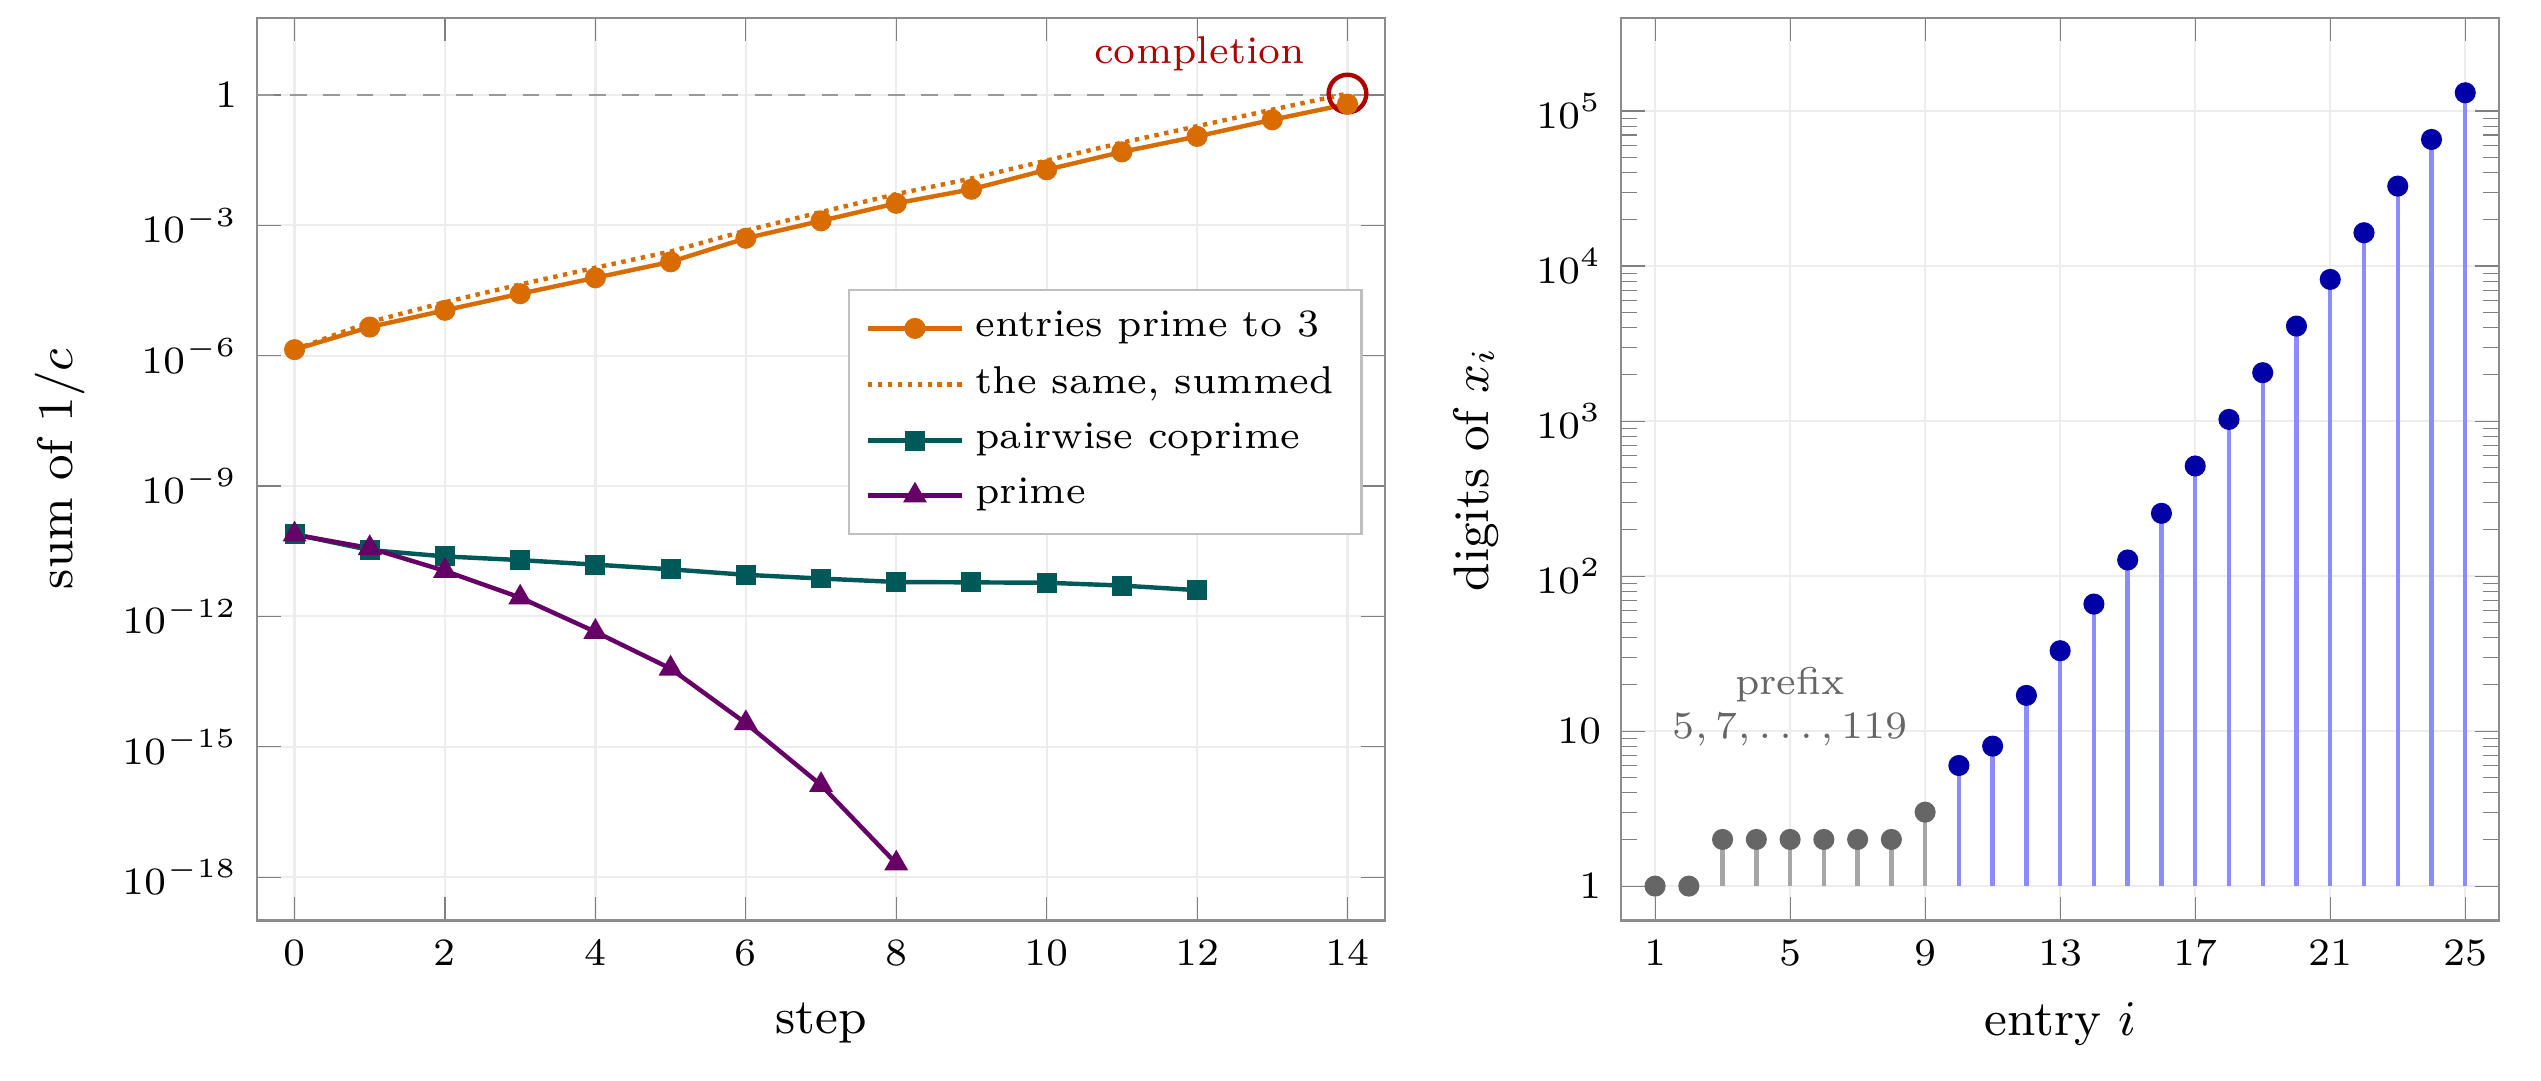
\includegraphics[width=\textwidth]{figures/fig_descent.png}
\caption{Left: the search for pseudo-solutions prime to $3$. The sum of
$1/c$ over the prefixes kept at each step estimates the number of
completions at that step. With $10^7$ prefixes kept it grows from
$1.4\cdot10^{-6}$ to $0.62$, its running total passes $1$ at step $14$,
and the tuple of Theorem~\ref{thm:pseudo25} is completed there. With
pairwise coprime entries and $10^6$ prefixes kept it falls from
$7.7\cdot10^{-11}$ to $4.0\cdot10^{-12}$ in twelve steps, and with
prime entries and $5000$ prefixes kept it falls from
$7.6\cdot10^{-11}$ to $2.1\cdot10^{-18}$ in eight
(Section~\ref{sec:largest}). Right: the
number of digits of the $25$ entries of that tuple, of which the first
nine form the prefix $5,7,13,17,19,23,25,37,119$.}
\label{fig:descent}
\end{figure}

None of these tuples has pairwise coprime entries, and the search
does not reach such tuples. Among the $910$ prefixes of length $9$ of
the tree for $k=13$ with positive defect the smallest defect is
$2529647$, while among the $48$ of them with pairwise coprime entries
it is $8544556193$. The traversal of the tree for $k=15$ with
pairwise coprime entries visits $63663$ nodes, and the $13190$
prefixes among them with $0<cx_j<2B$, which one more entry can
complete, have a sum of $1/c$ of $7.7\cdot10^{-11}$, against $1.4\cdot10^{-6}$ for the $26821$ prefixes from which the
search above started. Moreover only about seven per cent of the
children of a prefix are admissible and prime to every earlier entry,
against fourteen per cent without the second condition. Run from these
prefixes with $10^6$ children kept at each step, the search finds the
sum of $1/c$ falling by a factor of about $0.8$ per step, and no
completion in twelve steps.

Solutions of \eqref{eq:product} with $\varepsilon=+1$ give solutions
with $\varepsilon=-1$ through the analogue of
Theorem~\ref{thm:ext}(ii).

\begin{proposition}\label{prop:lehmerext}
Let $(x_1,\dots,x_k)$ satisfy \eqref{eq:product} with
$\varepsilon=+1$, let $A=x_1\cdots x_k$, and let $A^2+A-1=de$ with
$1\le d<e$. Then $(x_1,\dots,x_k,A+1+d,A+1+e)$ satisfies
\eqref{eq:product} with $\varepsilon=-1$. If $x_1,\dots,x_k$ are
pairwise coprime, then so are all $k+2$ entries if and only if
$\gcd(d^2-1,A)=\gcd(d-1,A+2)=1$, and this fails whenever $3$ or $5$
divides $A$.
\end{proposition}

\begin{proof}
Write $X=A+1+d$ and $Y=A+1+e$. Since $2\prod_i(x_i-1)=A+1$, the
equation for the longer tuple reads $AXY-1=(A+1)(X-1)(Y-1)$, which is
equivalent to $(X-A-1)(Y-A-1)=A^2+A-1$, as in the proof of
Theorem~\ref{thm:ext}; the entries increase because $x_k\le A<X<Y$.
Since $de\equiv-1\pmod A$, the integer $d$ is prime to $A$, so
$\gcd(X,A)=\gcd(d+1,A)$ and $\gcd(Y,A)=\gcd(d(e+1),A)=\gcd(d-1,A)$.
A prime $r$ dividing $X$ and $Y$ has $d\equiv e\equiv-(A+1)$, hence
$(A+1)^2\equiv A^2+A-1$, that is $A\equiv-2$ and $d\equiv1\pmod r$;
conversely, if $r$ divides $A+2$ and $d-1$, then
$e\equiv de=A^2+A-1\equiv1$, and $r$ divides $X$ and $Y$. If $3\mid A$,
then $A^2+A-1\equiv-1\pmod3$, so $3\nmid d$ and $3\mid d^2-1$. Finally
let $5\mid A$. Every prime factor $r$ of $A^2+A-1$ is odd and different
from $5$, and $(2A+1)^2\equiv5\pmod r$, so $5$ is a square modulo $r$
and, by quadratic reciprocity,\footnote{For an odd prime $r\ne5$ the
law of quadratic reciprocity gives $\bigl(\frac5r\bigr)=\bigl(\frac
r5\bigr)$, since $5\equiv1\pmod4$, and the nonzero squares modulo $5$
are $1$ and $4$.} $r\equiv\pm1\pmod5$. Hence
$d\equiv\pm1\pmod5$, and $5$ divides $\gcd(d^2-1,A)$.
\end{proof}

For the Fermat numbers $3,5,17,257,65537,2^{32}+1$,
Proposition~\ref{prop:lehmerext} gives pseudo-solutions of Lehmer's
equation with $\nu=2$, and none with pairwise coprime entries, because
$3$ divides $A$. Appending $2B+1=A+2$, as in the proof of
Theorem~\ref{thm:pseudo25}, keeps the entries pairwise coprime, so a
pairwise coprime pseudo-solution of the companion equation
prime to $3$ with $3\mid B$ gives infinitely many, and
Proposition~\ref{prop:lehmerext} turns every divisor $d$ of $A^2+A-1$
with $\gcd(d^2-1,A)=\gcd(d-1,A+2)=1$ into a pseudo-solution of
Lehmer's equation with pairwise coprime entries. By
Lemma~\ref{lem:parity} a pseudo-solution of Lehmer's equation with
pairwise coprime entries is prime to $3$, and none has at most $13$
entries, by Proposition~\ref{prop:largest}(iii). The smallest $k$ with a pseudo-solution prime to $3$ lies
between $14$ and $25$ for $\varepsilon=+1$, and between $14$ and $26$
for $\varepsilon=-1$.

\subsection{Descent, three entries and Korselt's criterion}\label{sec:structure}
Equation~\eqref{eq:product} has degree one in each entry. If all
entries but $x$ are fixed, and $A'$ and $B'$ are the products of the
other entries and of the numbers $x_j-1$ for them, then the equation
reads
\[
  x\,(2B'-A')=2B'+\varepsilon ,
\]
so the remaining entry is determined by the others, and it exists
exactly when $2B'-A'$ is positive and divides $2B'+\varepsilon$. This
is the step that completes a prefix in the search above. It also means
that the equation has no counterpart of the involution behind descent
arguments for equations of degree two in each variable.\footnote{For
Markov's equation $x^2+y^2+z^2=3xyz$, fixing $y$ and $z$ leaves a
quadratic equation in $x$ with the roots $x$ and $3yz-x$. Replacing the
largest entry of a solution by the other root gives a smaller
solution, and every solution descends in this way to $(1,1,1)$.}
Fixing $k-1$ entries leaves at most one solution, so there is no
second root to replace an entry with, and a descent of this kind has
nothing to act on.

The last two entries are easier to find than the last three for a
structural reason. By Proposition~\ref{prop:last}, the equation for the
last two entries after a prefix with products $A$ and $B$ is a product
of two linear forms set equal to the constant $2AB+\varepsilon C$, and
its solutions come from the divisors of that integer. With three
entries left this never happens.

\begin{proposition}\label{prop:threeentries}
Let $A$ and $B$ be positive integers with $C=2B-A>0$, and let
\[
  F(x,y,z)=Axyz+\varepsilon-2B(x-1)(y-1)(z-1),
\]
so that $x,y,z$ complete a prefix with products $A$ and $B$ exactly
when $F(x,y,z)=0$.
\begin{enumerate}[label=\textup{(\roman*)}]
\item With $u=Cx-2B$, $v=Cy-2B$ and $w=Cz-2B$,
\[
  uvw-2AB(u+v+w)=12AB^2-8B^3+(2B+\varepsilon)C^2-C^2F(x,y,z).
\]
\item There are no linear polynomials $L_1,L_2,L_3$ in $x,y,z$ with
rational coefficients and no rational number $\kappa$ with
$F=L_1L_2L_3+\kappa$.
\end{enumerate}
\end{proposition}

\begin{proof}
Write $e_1=x+y+z$ and $e_2=xy+yz+zx$. Expanding,
$F=-Cxyz+2Be_2-2Be_1+2B+\varepsilon$, and
\[
  uvw=C^3xyz-2BC^2e_2+4B^2Ce_1-8B^3,\qquad u+v+w=Ce_1-6B .
\]
Since $4B^2C-2ABC=2BC^2$, the left side of (i) equals
$C^2(Cxyz-2Be_2+2Be_1)-8B^3+12AB^2$, and
$Cxyz-2Be_2+2Be_1=2B+\varepsilon-F$. This proves (i).

For (ii), suppose that $F=L_1L_2L_3+\kappa$. The terms of degree three
give $\ell_1\ell_2\ell_3=-Cxyz$ for the homogeneous linear parts
$\ell_i$ of the $L_i$, and by unique factorisation each $\ell_i$ is a
rational multiple of one of $x$, $y$, $z$, a different one for each
$i$. So $F=\alpha(x+r)(y+s)(z+t)+\kappa$ with rational $\alpha,r,s,t$.
Comparing the coefficients of $xyz$, of $xy$, $yz$, $zx$, and of $x$
gives $\alpha=-C$, then $\alpha t=\alpha r=\alpha s=2B$, and finally
$\alpha st=-2B$. Hence $s=t=-2B/C$ and $-4B^2/C=-2B$, that is,
$C=2B$ and $A=0$, which is impossible.
\end{proof}

Part (i) shows what takes the place of the hyperbola
\eqref{eq:hyperbola}: the product $uvw$ is no longer a fixed integer but
moves with $u+v+w$, and by (ii) no choice of linear forms turns it into
one. The divisors of a single integer therefore do not give the last
three primes. This is why, for $k=16$, every admissible $p_{14}$ has to
be enumerated in Section~\ref{sec:sixteen}, and why a method that
treats a whole range of primes at once has to rest on something other
than divisors.

Primality enters the search only through its primality tests. Let
$(x_1,\dots,x_k)$ satisfy \eqref{eq:product} and put
$A=x_1\cdots x_k$. Every $x_i-1$ divides
$2\prod_j(x_j-1)=A+\varepsilon$, so by Fermat's little theorem a prime
entry $x_i$ satisfies $a^{A+\varepsilon}\equiv1\pmod{x_i}$ for every
integer $a$ prime to $x_i$. For a composite entry this is a real
condition.

\begin{lemma}\label{lem:korselt}
Let $(x_1,\dots,x_k)$ satisfy \eqref{eq:product}, put
$A=x_1\cdots x_k$, and let $x$ be an entry with
$a^{A+\varepsilon}\equiv1\pmod x$ for every integer $a$ prime to $x$.
Then $x$ is squarefree, and $q-1\mid A+\varepsilon$ for every prime
$q\mid x$. If the entries are pairwise coprime and each of them has
this property, then $A$ is squarefree and $q-1\mid A+\varepsilon$ for
every prime $q\mid A$; for $\varepsilon=-1$ and $k\ge2$ this says, by
Korselt's criterion, that $A$ is a Carmichael number.
\end{lemma}

\begin{proof}
Since $x\mid A$ and $\gcd(A,A+\varepsilon)=1$, no prime factor of $x$
divides $A+\varepsilon$. Let $q$ be a prime factor of $x$. If
$q^2\mid x$, the Chinese remainder theorem gives an integer $a$ prime
to $x$ with $a\equiv1+q\pmod{q^2}$, and then
$1\equiv a^{A+\varepsilon}\equiv1+(A+\varepsilon)q\pmod{q^2}$, so
$q\mid A+\varepsilon$, which is impossible. Hence $x$ is squarefree.
Taking instead for $a$ an integer prime to $x$ that is a primitive root
modulo $q$ gives $q-1\mid A+\varepsilon$. For pairwise coprime entries
the prime factors of $A$ are those of the entries, each to the first
power, which gives the last statement.
\end{proof}

The tuples constructed in the proof of Theorem~\ref{thm:pseudo25}
lack the property, since each of them contains the entry $25$, which
is not squarefree. In the tuple with $25$ entries it fails at other
entries as well: $147563=13\cdot11351$ and
$45571237=17\cdot2680661$ have the prime factors $11351$ and
$2680661$, for which $q-1$ does not divide $A+1$, and each of the
fourteen larger entries, all of them composite, has
$2^{A+1}\not\equiv1\pmod{x_i}$. Of the composite entries only
$119=7\cdot17$ has the property, as $6$ and $16$ divide $A+1$. For the
pseudo-solution $(3,5,17,257,65537,2^{32}+1)$ of the companion
equation, where $A+1=2^{64}$, the property fails at the last entry,
since $2^{32}+1=641\cdot6700417$ and $640\nmid2^{64}$; this is the
factorisation that excludes it in Section~\ref{sec:allk}.

Lemma~\ref{lem:korselt} therefore singles out a class of tuples
between the integer tuples of Section~\ref{sec:allk} and the prime
ones. The prime factors of a solution of \eqref{eq:first} or
\eqref{eq:second} with $M=2$ and $3\nmid n$ form a solution of
\eqref{eq:product} in pairwise coprime odd integers prime to $3$, each
of which satisfies $a^{A+\varepsilon}\equiv1\pmod{x_i}$ for every $a$
prime to $x_i$. No tuple in this section has these properties: those
of Propositions~\ref{prop:pseudo} and~\ref{prop:lehmerext} and of
Theorem~\ref{thm:pseudo25}, and the spoof factorisations above, all
have two entries with a common factor or contain the entry $3$. For
$k\le13$ no such tuple exists, by Theorem~\ref{thm:pseudo3}.

\subsection{Primality of the largest entry}\label{sec:largest}
The tuples of Sections~\ref{sec:allk} and~\ref{sec:structure}
weaken the primality of every entry. Here we keep the primality of
every entry but the largest and drop it there. The largest entry is the
one that the step at the start of Section~\ref{sec:structure}
determines from the others, and in the tuple
$(3,5,17,257,65537,2^{32}+1)$ of Section~\ref{sec:allk} it is the entry
whose primality decides the matter.

In the next lemma and the remarks after it, $p_1<\dots<p_j$, with $j\ge1$, are odd primes
with $p_i\nmid p_l-1$ for all $i$ and $l$, and
\[
  A=p_1\cdots p_j,\qquad B=(p_1-1)\cdots(p_j-1),\qquad C=2B-A .
\]
A prime factor of $A$ that divides $B$ divides some $p_l-1$, so
$\gcd(A,B)=1$.

\begin{lemma}\label{lem:largest}
If $C\ge1$, then $\gcd(C,2AB)=1$. Suppose moreover that $C$ divides
$2B+\varepsilon$, and put $X=(2B+\varepsilon)/C$.
\begin{enumerate}[label=\textup{(\roman*)}]
\item $X-1=(A+\varepsilon)/C$ and $\gcd(X,2B)=\gcd(X-1,A)=1$.
\item If $C=1$, then $X=A$ for $\varepsilon=-1$ and $X=A+2$ for
$\varepsilon=+1$.
\item Let $\varepsilon=-1$. If $3\mid A$, then $3\mid X$. If $3\nmid A$,
then $3\nmid X$ and $3\nmid C$.
\end{enumerate}
\end{lemma}

\begin{proof}
Since $\gcd(A,B)=1$, we have $\gcd(C,B)=\gcd(A,B)=1$ and
$\gcd(C,A)=\gcd(2B,A)=1$, and $C$ is odd because $A$ is.

(i) From $CX=2B+\varepsilon$ we get $C(X-1)=2B+\varepsilon-C=A+\varepsilon$. So
$X$ divides $2B+\varepsilon$, which is prime to $2B$, and $X-1$ divides
$A+\varepsilon$, which is prime to $A$.

(ii) If $C=1$, then $A=2B-1$ and $X=2B+\varepsilon=A+1+\varepsilon$.

(iii) If $3\mid A$, then $3$ is one of the $p_i$, and every other $p_l$
is congruent to $2$ modulo $3$, since $3\nmid p_l-1$. Hence
$B\equiv2$, $2B-1\equiv0$ and $C=2B-A\equiv1\pmod3$, and $3\mid X$. If
$3\nmid A$, then either some $p_l\equiv1\pmod3$ and $3\mid B$, or every
$p_l\equiv2\pmod3$ and $B\equiv1\pmod3$. In both cases $3\nmid2B-1=CX$.
\end{proof}

By the step at the start of Section~\ref{sec:structure}, a prime
$p>p_j$ makes $n=Ap$ a solution of $n-1=2\varphi(n)$ exactly when
$C\ge1$, $C$ divides $2B-1$ and $p=X$. Since $2B-1=C+(A-1)$, the
condition on the first $j$ primes is the single divisibility
$C\mid A-1$, and the only further condition is that $X$ be prime. This
is the congruence of the remark after Proposition~\ref{prop:local},
whose modulus depends on the prefix. Once $C$ divides $A-1$ the identity
$AX-1=2B(X-1)$ holds exactly, so every condition that Lehmer's equation
imposes modulo a power of a prime $q$ is contained in this one
divisibility, including $v_q(n-1)\ge\sum_iv_q(p_i-1)$, which Korselt's
criterion weakens to the largest of these valuations. For
$\varepsilon=-1$, part~(ii) is Proposition~\ref{prop:pseudo} read from
the prefix, and part~(iii) gives the case $M=2$ of
Lemma~\ref{lem:three}.

The next proposition asks nothing of the largest entry except that it
be prime to the others. Its first part holds for every $k$.

\begin{proposition}\label{prop:largest}
Let $k\ge2$, let $p_1<\dots<p_{k-1}$ be odd primes, and let $x>p_{k-1}$
be an integer prime to $p_1\cdots p_{k-1}$.
\begin{enumerate}[label=\textup{(\roman*)}]
\item If $(p_1,\dots,p_{k-1},x)$ satisfies \eqref{eq:product} with
$\varepsilon=-1$, then $p_i\nmid p_l-1$ for all $i$ and $l$, and, with
$A$, $B$ and $C$ formed from $p_1,\dots,p_{k-1}$, we have $3\nmid A$,
$C\ge5$, $C\mid A-1$ and $x=(2B-1)/C$. This holds with $x=p_k$ for
every composite solution $n=p_1\cdots p_k$ of $n-1=2\varphi(n)$.
\item If $k\le15$, then $(p_1,\dots,p_{k-1},x)$ does not satisfy
\eqref{eq:product} with $\varepsilon=-1$.
\item For $k\le13$, equation~\eqref{eq:product} with $\varepsilon=-1$
has no solution in pairwise coprime integers greater than $1$.
\end{enumerate}
\end{proposition}

\begin{proof}
(i) Put $A=p_1\cdots p_{k-1}$ and $B=(p_1-1)\cdots(p_{k-1}-1)$. A
common divisor of $Ax$ and $B(x-1)$ divides $Ax-2B(x-1)=1$, so
$\gcd(A,B)=1$ and $p_i\nmid p_l-1$ for all $i$ and $l$, and the
equation reads $Cx=2B-1$. So $C\ge1$, $C$ divides $2B-1=C+(A-1)$, hence
also $A-1$, and $x=X$ in the notation of Lemma~\ref{lem:largest}. Since
$x$ is prime to $A$, part~(iii) of that lemma gives $3\nmid A$ and
$3\nmid C$, and part~(ii) gives $C\ne1$, since $X=A$ is not prime to
$A>1$. As $C$ is odd, $C\ge5$. By Lemma~\ref{lem:basic}(i) a composite
solution of $n-1=2\varphi(n)$ is odd and squarefree, say
$n=p_1\cdots p_k$ with primes $p_1<\dots<p_k$ and $k\ge2$. Then
$n-1=2\prod_i(p_i-1)$, so $(p_1,\dots,p_k)$ satisfies
\eqref{eq:product} with $\varepsilon=-1$, and $x=p_k$ is prime to the
other entries.

(ii) Suppose that the tuple satisfies \eqref{eq:product} with
$\varepsilon=-1$ and $k\le15$. By part~(i), $3\nmid A$, and
Lemma~\ref{lem:largest}(iii) gives $3\nmid x$.
The entries are odd, since $x$ divides $2B-1$, and increasing, and
they satisfy \eqref{eq:product} with $\varepsilon=-1$ and hence the
conditions $\gcd(x_i,x_l-1)=1$. If $x$ is prime,
then $Ax$ is a composite solution of $\varphi(n)\mid n-1$ with at most
fifteen prime factors, which Theorem~\ref{thm:first} excludes.
Otherwise the tuple is a pseudo-solution prime to $3$ whose first $k-3$
entries are prime, which Theorem~\ref{thm:pseudo3}(ii) excludes.

(iii) Let pairwise coprime integers greater than $1$ form such a
solution. They are odd, since an
even entry would make the left side of \eqref{eq:product} odd and the
right side even. By Lemma~\ref{lem:parity} the number of entries
divisible by $3$ is even, and pairwise coprime entries include at most
one multiple of $3$, so no entry is divisible by $3$. If every entry is
prime, Theorem~\ref{thm:first} excludes the solution; otherwise it is a
pseudo-solution prime to $3$, which Theorem~\ref{thm:pseudo3}(i)
excludes.
\end{proof}

For the companion equation the analogue of
Proposition~\ref{prop:largest}(ii) is false. The tuple
$(3,5,17,257,\allowbreak65537,2^{32}+1)$ of Section~\ref{sec:allk} has five prime
entries, and its last entry $2^{32}+1=641\cdot6700417$ is prime to
them. With $A=2^{32}-1$ and $B=2^{31}$ it satisfies
$Ax+1=2^{64}=2B(x-1)$, which is \eqref{eq:product} with
$\varepsilon=+1$. It comes from $C=1$, which by
Lemma~\ref{lem:largest}(ii) gives the entry $A+2$ for $\varepsilon=+1$.
For $\varepsilon=-1$ the same step gives the entry $A$, which is not
prime to the others; it produces the pseudo-solutions of
Proposition~\ref{prop:pseudo} and those of Theorem~\ref{thm:pseudo25}
with $\varepsilon=-1$, and the condition $C\ge5$ of
Proposition~\ref{prop:largest}(i) excludes it.

Proposition~\ref{prop:largest}(ii) rests on the searches, and they give
no shortcut beyond $k=15$. After a prefix of $k-2$ primes, with $A$, $B$
and $C$ now formed from these, the identity \eqref{eq:hyperbola}, whose
proof uses only the equation, turns the last two entries $y<x$ into a
factorisation $(Cy-2B)(Cx-2B)=2AB-C$, and
Proposition~\ref{prop:largest}(ii) asks only that $y$ be prime and $x$
be prime to the other entries. Its extension to $k=16$ therefore needs
the traversal of Section~\ref{sec:sixteen}, with its
$9\cdot10^{13}$ two-prime problems.

The next lemma shows how the primality of the prefix keeps the
defects large.

\begin{lemma}\label{lem:defect}
Let $x_1<\dots<x_j$ be integers greater than $1$ with
$A=x_1\cdots x_j$ and $B=(x_1-1)\cdots(x_j-1)$, suppose that
$C=2B-A\ge2$ is prime to $2B$, and put $y_0=\lfloor2B/C\rfloor+1$. An
entry $y$ appended to the prefix gives a positive defect exactly when
$y\ge y_0$, and then
\[
  Cy-2B=r+(y-y_0)C,\qquad r=Cy_0-2B,\qquad 1\le r\le C-1 .
\]
In particular the defect decreases only for $y=y_0$. Moreover $C$
divides $2B-1$ exactly when $r=C-1$, and then $(2B-1)/C=y_0-1$.
\end{lemma}

\begin{proof}
Appending $y$ gives the defect $2B(y-1)-Ay=Cy-2B$, which is positive
exactly when $y>2B/C$, that is, when $y\ge y_0$. Since $C\ge2$ is prime
to $2B$, it does not divide $2B$, so $r=C-(2B\bmod C)$ lies between $1$
and $C-1$. Finally $r=C-1$ exactly when $2B\bmod C=1$, that is, when
$C\mid2B-1$, and then $2B-1=C\lfloor2B/C\rfloor=C(y_0-1)$.
\end{proof}

Along a path of integers every step may take the entry $y_0$, and the
defects can fall quickly: in the search behind
Theorem~\ref{thm:pseudo25} the smallest defect fell from
$1.9\cdot10^6$ after the first step to $29$ at the fourteenth. Along a
path of independent primes, where $\gcd(C,2B)=1$ by
Lemma~\ref{lem:largest}, the defect falls only at a step where
$\lfloor2B/C\rfloor+1$ happens to be prime. Of the $13190$ prefixes
from which the search with pairwise coprime entries starts, $12170$
consist of primes, with a sum of $1/C$ of $7.6\cdot10^{-11}$. A search
of the same kind in which every new entry is a probable prime, started
from these
$12170$ prefixes and keeping at each step the $5000$ children with the
smallest defect, saw the smallest defect rise from $1.2\cdot10^{11}$ to
$2.2\cdot10^{18}$ in eight steps. The sum of $1/C$, which estimates the
number of completions by an integer, fell to $2.1\cdot10^{-18}$, with a
total of $1.3\cdot10^{-10}$ over all steps and no completion
(Figure~\ref{fig:descent}). With integer entries, as in the search
behind Theorem~\ref{thm:pseudo25}, and the same prefixes and number of
children, the sum rose instead, to a total of $1.9\cdot10^{-8}$ after
twelve steps. These counts are heuristic, and no result of this
paper depends on them.

For Lehmer's equation with $M=2$ the tuples of this section compare
as follows. The prime factors of a composite solution of
$n-1=2\varphi(n)$ form a solution of \eqref{eq:product} with
$\varepsilon=-1$ of each of three kinds: in odd integers prime to $3$;
in pairwise coprime odd integers that pass the test of
Lemma~\ref{lem:korselt}; and in primes followed by a largest entry
prime to them. Solutions of the first kind exist for every $k\ge26$
(Theorem~\ref{thm:pseudo25}). Solutions of the second and third kinds
have pairwise coprime entries, so none has $k\le13$
(Proposition~\ref{prop:largest}(iii)), and none of the third kind has
$k\le15$ (Proposition~\ref{prop:largest}(ii)). Neither of these two
kinds contains the other: the second asks of every entry a property
weaker than primality, and the third asks every entry but the largest
to be prime and nothing of the largest except that it be prime to the
others. By Proposition~\ref{prop:largest}(i) a solution of the third
kind comes from a prefix of independent odd primes with $C\ge5$,
$C<(2B-1)/p_{k-1}$ and $C\mid2B-1$. By Proposition~\ref{prop:local} no
congruence modulo a fixed number other than that of
Lemma~\ref{lem:three} removes a prefix with two or more entries left,
so excluding these prefixes for $k\ge16$ needs the modulus $C$ of each
prefix.

\subsection{Prime factors of the last defect}\label{sec:defect}
Let $n=p_1\cdots p_k$ be a composite solution of $n-1=2\varphi(n)$, and
form $A$, $B$ and $C$ from $p_1,\dots,p_{k-1}$ as in
Section~\ref{sec:largest}. We call $C$ the \emph{last defect} of $n$.
By Proposition~\ref{prop:largest}(i), $C\ge5$, $C\mid A-1$ and
$p_k=(2B-1)/C$, so the first $k-1$ prime factors determine the last
through $C$ (Figure~\ref{fig:defect}). By Corollary~\ref{cor:indep},
every composite solution of $\varphi(n)\mid n-1$ with at most $16000$
prime factors satisfies $n-1=2\varphi(n)$ and is prime to $3$. The
prime factors of $C$ restrict the other prime factors of $n$ in the way
that the prime $3$ does in Lemma~\ref{lem:three}.

\begin{lemma}\label{lem:ell}
Let $n=p_1\cdots p_k$ be a composite solution of $n-1=2\varphi(n)$
with last defect $C$, and let $\ell$ be a prime factor of $C$.
\begin{enumerate}[label=\textup{(\roman*)}]
\item $\ell\ne p_i$ and $p_i\not\equiv1\pmod\ell$ for every $i<k$.
\item $A\equiv1$ and $2B\equiv1\pmod C$, so that
$\prod_{i<k}(1-1/p_i)\equiv\frac12\pmod C$.
\item $\displaystyle\prod_{i<k}\frac{p_i}{p_i-1}<2<\prod_{i\le k}\frac{p_i}{p_i-1}$.
\end{enumerate}
\end{lemma}

\begin{proof}
By Lemma~\ref{lem:largest}, $\gcd(C,2AB)=1$. (i) The prime $\ell$
divides neither $A=p_1\cdots p_{k-1}$ nor $B=(p_1-1)\cdots(p_{k-1}-1)$.
(ii) The first congruence is $C\mid A-1$, and the second is
$2B-1=p_kC$. As $A$ and $B$ are prime to $C$, the product
$\prod_{i<k}(1-1/p_i)=B/A$ is congruent to $\frac12$ modulo $C$.
(iii) The product over $i<k$ is $A/B=2-C/B<2$, and the product over
$i\le k$ is $n/\varphi(n)=2+1/\varphi(n)$ by
Lemma~\ref{lem:basic}(iii).
\end{proof}

\begin{figure}[t]
\centering
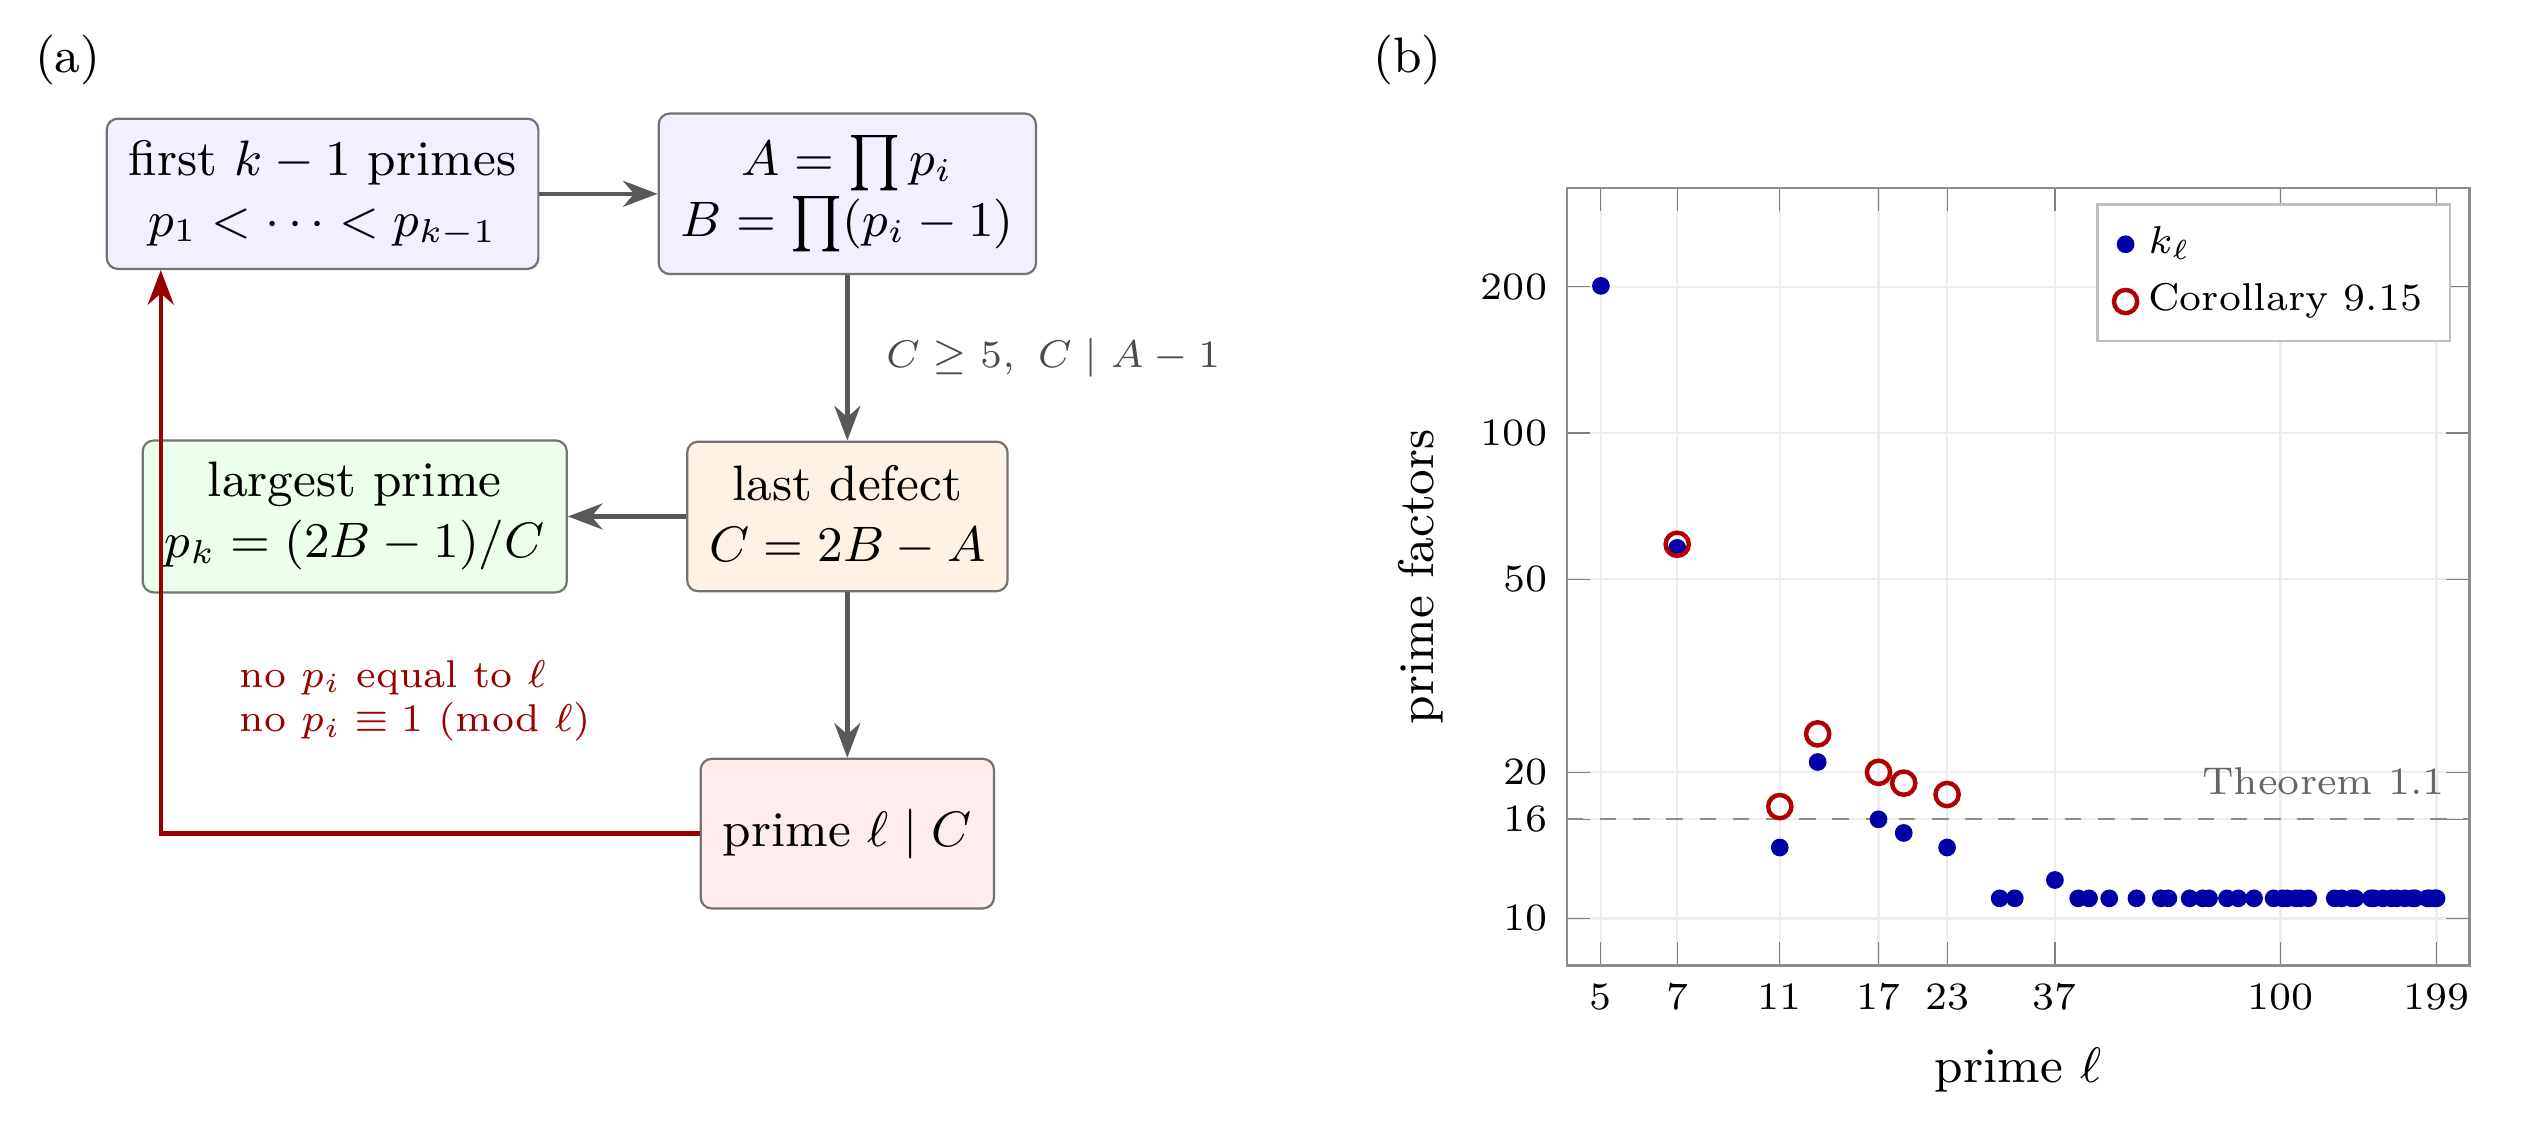
\includegraphics[width=\textwidth]{figures/fig_defect.png}
\caption{(a)~The first $k-1$ prime factors of a solution of
$n-1=2\varphi(n)$ determine $A$, $B$ and the last defect $C$, and $C$
determines the largest prime factor. A prime $\ell$ dividing $C$
excludes $\ell$ and the class $1$ modulo $\ell$ from the first $k-1$
prime factors (Lemma~\ref{lem:ell}). (b)~The least number $k_\ell$ of
prime factors that this exclusion allows, for the primes $\ell\le199$
(Proposition~\ref{prop:kell}), and the larger lower bounds of
Corollary~\ref{cor:defect} (open circles). The dashed line is the bound
$\omega(n)\ge16$ of Theorem~\ref{thm:first}.}
\label{fig:defect}
\end{figure}

Part~(i) removes from the first $k-1$ prime factors the prime $\ell$
and the primes congruent to $1$ modulo $\ell$, which by the prime number
theorem for arithmetic progressions make up the proportion $1/(\ell-1)$
of all primes, and part~(iii) then needs many of the primes that
remain. To measure this, let $\ell\ge5$ be prime and
$K\ge1$. We call a set $S$ of $K$ primes an \emph{$\ell$-set} if its
elements are at least $5$, different from $\ell$ and not congruent to
$1$ modulo $\ell$, if $S$ is independent, and if
\begin{equation}\label{eq:lset}
  \prod_{p\in S}\frac{p}{p-1}<2<\prod_{p\in S}\frac{p}{p-1}\cdot\frac{q_S}{q_S-1},
\end{equation}
where $q_S$ is the least prime larger than the elements of $S$ that is
not congruent to $1$ modulo any of them. Let $k_\ell$ be the least
value of $K+1$ for which an $\ell$-set of size $K$ exists. If $\ell$
divides the last defect of a solution $n=p_1\cdots p_k$, then
$S=\{p_1,\dots,p_{k-1}\}$ is an $\ell$-set: its elements are at least
$5$ by Proposition~\ref{prop:largest}(i), it is independent by
Lemma~\ref{lem:basic}(ii), Lemma~\ref{lem:ell}(i) gives the conditions
modulo $\ell$, and $p_k\ge q_S$, because $p_k$ is a prime larger than
$p_{k-1}$ and not congruent to $1$ modulo any $p_i$, so that
Lemma~\ref{lem:ell}(iii) gives \eqref{eq:lset}. Hence $k\ge k_\ell$.

\begin{proposition}\label{prop:kell}
We have $k_5=201$, $k_7=58$, $k_{11}=14$, $k_{13}=21$, $k_{17}=16$,
$k_{19}=15$, $k_{23}=14$ and $k_{37}=12$, and $k_\ell=11$ for every
other prime $\ell$ with $29\le\ell\le199$. A composite solution of
$n-1=2\varphi(n)$ whose last defect is divisible by $\ell$ has at least
$k_\ell$ prime factors.
\end{proposition}

\begin{proof}
The second assertion was shown above. For the first we use the search
of Proposition~\ref{prop:indep} with three changes. The allowed primes
are those from $5$ on that differ from $\ell$ and are not congruent to
$1$ modulo $\ell$. The bound $B(S)$ of a set $S$ with fewer than $K$
elements contains, besides the factors for $S$ and for the $K-|S|$
smallest candidates for $S$, the factor $q/(q-1)$ for the least prime
$q$ above the last of these candidates that is not congruent to $1$
modulo an element of $S$; this prime is not restricted modulo $\ell$,
since Lemma~\ref{lem:ell} says nothing about $p_k$ modulo $\ell$.
Finally, a set whose product is at least $2$ is discarded, since every
set that contains it has a larger product. If $T$ is an $\ell$-set of
size $K$ whose $|S|$ smallest elements form $S$, then the other
elements of $T$ are candidates for $S$ and $q_T$ is at least the prime
$q$ just described, so the right-hand side of \eqref{eq:lset} for $T$
is at most $B(S)$, and the argument in the proof of
Proposition~\ref{prop:indep} shows that the search creates $T$. For
every $\ell$ the search finds no $\ell$-set of size less than
$k_\ell-1$ and finds one of size $k_\ell-1$.\footnote{For $\ell=17$ the
only $\ell$-set of size $15$ is
$\{5,7,13,19,23,37,59,67,73,83,89,97,107,109,163\}$, with $q_S=173$ and
product $1.98918\ldots$; its last defect
$C=15724416449794753166951$ is congruent to $6$ modulo $17$.} Sets of
size $K$ are decided by \eqref{eq:lset} in exact rational arithmetic,
and the bounds are handled as in Proposition~\ref{prop:indep}, so that
rounding can add sets to the search but never remove one. Two programs
written independently carry out the search
(Appendix~\ref{app:defect}).
\end{proof}

For $\ell=11$ and for $17\le\ell\le199$ the value of $k_\ell$ is at most the
bound $16$ of Theorem~\ref{thm:first}. Deciding the equation on every
$\ell$-set goes further.

\begin{proposition}\label{prop:defectk}
For each pair $(\ell,k)$ in Table~\ref{tab:defect}, no composite
solution of $n-1=2\varphi(n)$ with $k$ prime factors has a last defect
divisible by $\ell$.
\end{proposition}

\begin{proof}
For such a solution $\{p_1,\dots,p_{k-1}\}$ is an $\ell$-set of size
$k-1$, as shown above, and with $A$, $B$ and $C$ formed from its
elements, $\ell$ divides $C$ and $C$ divides $A-1$. Continued past the
first $\ell$-set, the search of Proposition~\ref{prop:kell} lists every
$\ell$-set of size $k-1$. Table~\ref{tab:defect} gives their number
and the number of them with $\ell\mid C$; none of these has
$C\mid A-1$.
\end{proof}

\begin{table}[t]
\centering
\caption{The $\ell$-sets of size $k-1$ for the pairs $(\ell,k)$ of
Proposition~\ref{prop:defectk}, and the number of them whose last
defect $C$ is divisible by $\ell$. None of them has $C\mid A-1$.}
\label{tab:defect}
\begin{tabular}{rrrr@{\qquad}rrrr}
\toprule
$\ell$ & $k$ & $\ell$-sets & $\ell\mid C$ & $\ell$ & $k$ & $\ell$-sets & $\ell\mid C$\\
\midrule
$7$ & $58$ & $70829$ & $11708$ & $19$ & $15$ & $1$ & $0$\\
$11$ & $14$ & $17$ & $2$ & $19$ & $16$ & $40$ & $1$\\
$11$ & $15$ & $803$ & $93$ & $19$ & $17$ & $1926$ & $113$\\
$11$ & $16$ & $582751$ & $61964$ & $19$ & $18$ & $319369$ & $17685$\\
$13$ & $21$ & $118$ & $12$ & $23$ & $14$ & $4$ & $0$\\
$13$ & $22$ & $11965$ & $974$ & $23$ & $15$ & $95$ & $4$\\
$13$ & $23$ & $3254401$ & $273205$ & $23$ & $16$ & $5348$ & $251$\\
$17$ & $16$ & $1$ & $0$ & $23$ & $17$ & $1766427$ & $81086$\\
$17$ & $17$ & $42$ & $1$ & & & &\\
$17$ & $18$ & $2836$ & $161$ & & & &\\
$17$ & $19$ & $935248$ & $59643$ & & & &\\
\bottomrule
\end{tabular}
\end{table}

\begin{corollary}\label{cor:defect}
Let $n$ be a composite solution of $\varphi(n)\mid n-1$ with $k\le16000$
prime factors. Then $n-1=2\varphi(n)$; let $C$ be its last defect.
\begin{enumerate}[label=\textup{(\roman*)}]
\item If $\ell\mid C$, then $k\ge201$ for $\ell=5$, $k\ge59$ for
$\ell=7$, $k\ge17$ for $\ell=11$, $k\ge24$ for $\ell=13$, $k\ge20$ for
$\ell=17$, $k\ge19$ for $\ell=19$ and $k\ge18$ for $\ell=23$.
\item If $k=16$, then every prime factor of $C$ is at least $29$; in
particular $C\ge29$.
\end{enumerate}
\end{corollary}

\begin{proof}
By Corollary~\ref{cor:indep}, $n-1=2\varphi(n)$. (i) Proposition~\ref{prop:kell} gives $k\ge k_\ell$, and
Proposition~\ref{prop:defectk} excludes the values of $k$ from $k_\ell$
up to one less than the stated bound. (ii) The number $C$ is odd, and
$3\nmid C$ by Lemma~\ref{lem:largest}(iii), since $3\nmid A$. For
$k=16$, part~(i) shows that no prime from $5$ to $23$ divides $C$. As
$C\ge5$, it has a prime factor, and every prime factor is at least
$29$.
\end{proof}

For the primes $\ell$ with $29\le\ell\le199$ the values of $k_\ell$ lie
below the bound of Theorem~\ref{thm:first}, and Lemma~\ref{lem:ell}
bounds the prime factors of $C$ only from below. A solution with
sixteen prime factors whose last defect has only prime factors from
$29$ on is therefore not excluded by this section; excluding it needs
the traversal of Section~\ref{sec:sixteen}.

\begin{remark}\label{rem:open}
Lehmer's conjecture is equivalent to the following assertion, which
this paper does not prove: \emph{there are no finite set $S$ of odd
primes and no integer $M\ge2$ such that, with $A=\prod_{p\in S}p$ and
$B=\prod_{p\in S}(p-1)$, the number $D=MB-A$ is positive, divides
$A-1$, and makes $(MB-1)/D$ a prime larger than every element of $S$.}
Indeed, let $n$ be a composite solution of $\varphi(n)\mid n-1$, let
$q$ be its largest prime factor, $S$ the set of its other prime factors
and $M=(n-1)/\varphi(n)$. Then $n=Aq$, $\varphi(n)=B(q-1)$, and
$n-1=M\varphi(n)$ reads $qD=MB-1$; so $D\ge1$, $D$ divides
$MB-1=D+(A-1)$ and hence $A-1$, and $q=(MB-1)/D$. Conversely, for $S$
and $M$ as in the assertion the number $n=Aq$ with $q=(MB-1)/D$ is
composite and satisfies $n-1=M\varphi(n)$, since $qD=MB-1$ is the same
equation. By Theorem~\ref{thm:first} a set $S$ with these properties
has at least $15$ elements, at least $16000$ if $M\ge3$, and at least
$10^8$ if $3\in S$. For $M=2$ the number $D$ is the last defect, with
the properties of Proposition~\ref{prop:largest}(i) and
Corollary~\ref{cor:defect}. The assertion asks that one number attached
to each set $S$ never be a prime above the elements of $S$. The
integer tuples of Theorem~\ref{thm:pseudo25} show that a proof has to
use the primality of the elements of $S$, and
Proposition~\ref{prop:local} shows that no congruence modulo a fixed
number other than that of Lemma~\ref{lem:three} can replace the
modulus $D$, which depends on $S$. For the companion equation the same
construction with $D=1$ gives the Fermat numbers: the Fermat primes
$S=\{3,5,17,257,65537\}$ give $2^{32}+1$. For Lehmer's equation $D=1$
would give $(MB-1)/D=A$, which is not a prime larger than the elements
of $S$; so $D>1$, and the assertion is not a question about Fermat
numbers.
\end{remark}



\appendix
%%==================================================================
\section{Implementation and checks}\label{app:checks}
%%==================================================================

This appendix describes how the computations were carried out and
checked. None of it is used in the proofs beyond the statements of
Section~\ref{sec:checks}.


\subsection{Two implementations}\label{app:two}
The first implementation is recursive and works with exact rational
arithmetic. At a terminal node it enumerates $p_{k-1}$ over its
interval when the interval is short or $D$ is large, and otherwise
enumerates the divisors of $D$. The second was written separately. It
traverses the tree iteratively with an explicit stack, works only with
the integers $A_j$ and $B_j$, computes the interval endpoints from a
floating-point guess corrected by integer comparisons, and at every
terminal node enumerates $p_{k-1}$ over the whole interval. It never
factors anything. For Theorems~\ref{thm:first} and \ref{thm:coprime}
the second implementation is the proof and the first a corroboration.
For Theorem~\ref{thm:eight} with $k=7$ the roles are reversed, for the
reason given in Section~\ref{sec:seven}, and the factorisations used
are all certified. In every run the two implementations visited the
same number of nodes. For $k=15$ the route of Section~\ref{sec:sum},
which factors nothing, plays the part of the second implementation,
and the two lattice implementations of Section~\ref{sec:three}
corroborate it. The case $k=8$ of Theorem~\ref{thm:eight} rests on
the program of Section~\ref{sec:eight}, whose checks are described in
Section~\ref{sec:checks8}. The search behind Theorem~\ref{thm:size}
was likewise carried out by two independent programs
(Appendix~\ref{app:size}), and so were the searches of
Proposition~\ref{prop:indep} and of Section~\ref{sec:defect}
(Appendix~\ref{app:defect}).

\subsection{A second implementation of the lattice method}\label{app:second}
We implemented the lattice method twice. The first implementation
follows Section~\ref{sec:three}: its boxes are intervals in $u$, and the candidates
in a box come from Lemma~\ref{lem:firsthit}. The second takes its
nodes at depth $k-3$ from the rational bounds of the first program of
Appendix~\ref{app:two}, generates the primes $s$ by a different
routine, cuts the hyperbola into boxes along $v$ rather than $u$, and
lists the points of the coset in a box from a basis of the lattice
$\{(u,v):r'u+rv\equiv0\pmod c\}$ that is Lagrange-reduced for the norm
in which the box is a square;\footnote{A basis $e_1,e_2$ of a plane
lattice is Lagrange-reduced for a positive definite quadratic form $Q$
when $Q(e_1)\le Q(e_2)\le Q(e_2\pm e_1)$. For a box with sides $w_u$
and $w_v$ the program takes $Q(u,v)=(w_vu)^2+(w_uv)^2$, writes the
four corners of the box in the coordinates of the reduced basis, and
runs over the integer points of the smallest rectangle that contains
them. Since the box is convex, this rectangle contains the coordinates
of every lattice point in the box whatever the basis; the reduction
only keeps the rectangle small.} a point is accepted when it satisfies
\eqref{eq:uv} exactly. It switches to factoring at a lower threshold,
and it certifies every prime factor with FLINT. The two share no code
beyond the arithmetic libraries.

\subsection{Fifteen primes}\label{app:fifteen}
For the $33865004$ two-prime problems of Section~\ref{sec:fifteen},
the first lattice implementation factored $N$ completely in the $473$
cases where the estimated number of boxes exceeded its threshold, and
took $19$ minutes of processor time in all. The second factored $N$ in
$1772$ cases and took $45$ minutes. The route of
Section~\ref{sec:sum}, which factors nothing, took $13$ minutes
(Table~\ref{tab:k15}).

\begin{table}[ht]
\centering
\caption{The case $k=15$ of $n-1=2\varphi(n)$, by the two lattice
implementations of Section~\ref{sec:three} and the route of
Section~\ref{sec:sum}. The three agree on each of the $55443$ pieces
into which the work was divided.}
\label{tab:k15}
\smallskip
\begin{tabular}{@{}lrrr@{}}
\toprule
 & first & second & sums \\
\midrule
prefixes of twelve primes & $54\,985$ & $54\,985$ & $54\,985$ \\
admissible choices of $p_{13}$ & $33\,865\,004$ & $33\,865\,004$ & $33\,865\,004$ \\
boxes & $82\,882\,379$ & $61\,384\,414$ & -- \\
lattice points tested & $30\,664\,171$ & $25\,527\,573$ & -- \\
trial divisions & -- & -- & $116\,427\,765$ \\
square tests & -- & -- & $82\,568\,071$ \\
complete factorisations of $N$ & $473$ & $1\,772$ & $0$ \\
completions $s<p<q$ in integers & $0$ & $0$ & $0$ \\
processor time & 19 min & 45 min & 13 min \\
\bottomrule
\end{tabular}
\end{table}

\subsection{Equations with solutions}
Both implementations accept a general equation
\begin{equation}\label{eq:ab}
  b\,(n+\varepsilon)=a\,\varphi(n)
\end{equation}
with positive integers $a,b$, the bounds of
Section~\ref{sec:search} holding with $2$ replaced by $a/b$ and
\eqref{eq:hyperbola} becoming $(Cp-aB)(Cq-aB)=b(aAB+\varepsilon C)$
with $C=aB-bA$. For $\varepsilon=-1$, $b=2^k$ and $a=2^k+h$, equation
\eqref{eq:ab} says that $\varphi(n)/2^k=\prod_i\frac{p_i-1}{2}$
divides $n-1$ with quotient $2^k+h$, and it has solutions. We ran both implementations with
$p_{\min}=3$ for $k=4$, $1\le h\le40$, and for $k=5$, $1\le h\le85$.
Both returned the same $56$ solutions, $20$ with $k=4$ and $36$ with
$k=5$, listed in Appendix~\ref{app:known}; each was verified by direct
arithmetic. The bounds and prunes exercised here are exactly those on
which Theorems~\ref{thm:first}, \ref{thm:eight} and~\ref{thm:coprime} depend.

\subsection{A sieve}
As a check that shares no code with the search, we computed
$\varphi(n)$ for all $n\le10^8$ by a sieve. There is no composite
$n\le10^8$ with $\varphi(n)\mid n-1$; the $n\le10^8$ with
$\varphi(n)\mid n+1$ are $1,2,3,15,255,65535,83623935$; and the odd
squarefree $n\le10^8$ with $\omega(n)\in\{4,5\}$ satisfying
\eqref{eq:ab} for the parameters above are exactly the ten members of
the list in Appendix~\ref{app:known} below $10^8$.

\subsection{The known solutions}
For $\varepsilon=+1$ and $p_{\min}=3$ the search is its own test:
Table~\ref{tab:seven} shows that every known Fermat-type solution with
at most six prime factors is found, at the right depth, and nothing
else.

\subsection{The last three primes}\label{sec:checks3}
The methods of Section~\ref{sec:three} were checked in five ways.

\emph{Brute force.} The routines that list the divisors of $N$ in a
residue class were compared with the list read off from a known
factorisation. The two lattice routines were run on $4000$ and $3674$
random integers $N$ of up to $93$ digits, with up to seven prime
factors of up to thirteen digits, some of them repeated. The moduli $c$
had between $2$ and $55$ per cent of the bits of $N$, so that $c^3/N$
ranged from about $10^{-82}$ to $10^{44}$, and the classes were chosen
at random or among the classes of actual divisors. Of these instances
$2764$ and $2586$ were handled by boxes, and the rest, where the
number of boxes would have exceeded the limit, by the factoring
fallback. The sum route was run on $3100$ integers
$N\equiv r^2\pmod c$ of up to $46$ digits, about half of them
products of two planted members of the class, with $c^3/N$ between
about $10^{-13}$ and $10^{28}$. All lists agreed.

\emph{Planted divisors.} We took $1400$ pairs of a prefix and a prime
$s$ from the search, $400$ of them just above the lower ends of the
forty longest intervals, where $c^3/N$ is smallest, and replaced $N$ by
the product of two members $t\le t^*$ of the class of about the same
size, with $t$ chosen log-uniformly; the values of $c^3/N$ ranged from
$10^{-7.7}$ to $10^{15}$. The sum route found the planted divisor in
all $1400$ cases. The lattice routines were run with factoring switched
off, a limit of $20000$ boxes and a limit of five seconds per instance.
They found the planted divisor in $1287$ and $1210$ cases and stopped
at a limit in the others. Nothing they returned was wrong, and whenever
two routines finished they returned the same list. The time limit is
needed because $r'=r$ makes the coset \eqref{eq:coset} a union of
lines $u+v=\text{const}$. A planted divisor puts a long segment of
such a line inside the box that contains it, and the lattice routines
examine every point of that segment. This affects only the running
time, and the runs of the search had no time limit.

\emph{Equations with solutions.} Used as a complete search from depth
$k-3$, both lattice implementations return the $56$ solutions of
\eqref{eq:ab} for $k=4$ and $k=5$. For \eqref{eq:second} with
$p_{\min}=3$ and $3\le k\le7$ they return exactly the solutions
$255$, $65535$, $83623935$, $4294967295$ and $6992962672132095$ of
Table~\ref{tab:seven}, and nothing with $k=7$. Since every
factorisation in these runs is certified, this re-derives the case
$3\le k\le7$ of Theorem~\ref{thm:eight} independently of
Section~\ref{sec:seven}. The sum route, applied to the first $k-2$
primes of each of these $61$ solutions, returns the solution. For
$7\le k\le14$ and both signs of $\varepsilon$ all three find no
solution, and the number of choices of $p_{k-2}$ they treat equals the
number of nodes at depth $k-2$ found in Sections~\ref{sec:first}
and~\ref{sec:second}.

\emph{The lattice route alone.} For each of the $61$ known solutions
we took $s=p_{k-2}$ from the solution and asked the first
implementation, with factoring switched off, for the divisors of $N$ in
the class. In all $36$ cases with $c>1$ the divisor $t=cp_{k-1}-aB'$
was among them; when $c=1$ every integer lies in the class and only
factoring applies. The second implementation assumes $\gcd(r,c)=1$,
which holds in the search by Proposition~\ref{prop:class} but in only
one of these cases, and there it found $t$ as well.

\emph{Agreement.} For each sign of $\varepsilon$ the three
computations divided the case $k=15$ into the same $55443$ tasks,
counted the same number of primes $p_{13}$ in every task, and returned
no completion in integers in any task.

\subsection{The eight-prime search}\label{sec:checks8}
The computation of Section~\ref{sec:eight} was cut into $10897$
pieces, each a range of $s$ under one prefix, and run on four
processors. It made $3.4\cdot10^{11}$ trial divisions; the sums ranged
over $6.7\cdot10^{13}$ values of $\sigma$, and the sieve (iii) passed
$2.1\cdot10^{8}$ of them on to the exact test. The whole run took
$6.9$ hours of processor time, $3.2$ of them in PARI/GP.

The program was tested in four ways before the run, and part of the
run was repeated afterwards.

\emph{Known solutions.} Run with prime entries, $\varepsilon=+1$ and
$p_{\min}=3$ from depth $k-3$ for $3\le k\le7$, the program returns
the solutions $255$, $65535$, $83623935$, $4294967295$ and
$6992962672132095$, and no other completion with prime entries. The
runs were repeated with every divisor sent to the trial division (i),
with every divisor sent to the sum route (ii), and with the
multiprecision arithmetic used for every quantity; all runs return the
same completions among those in which $p$ and $q$ have no prime factor
up to $61$ other than themselves.

\emph{Odd integers.} With the conditions modulo $3$ removed, and with
the congruence prune of Theorem~\ref{thm:pseudo3} in place of the
conditions on primes, the program solves \eqref{eq:product} in odd
integers. For $3\le k\le7$ it finds $1$, $1$, $2$, $8$ and $47$
solutions with $\varepsilon=-1$, and $1$, $1$, $2$, $4$ and $18$ with
$\varepsilon=+1$, the numbers found by the independent program of
Theorem~\ref{thm:pseudo3}, and again all runs agree.

\emph{Complete factorisation.} We took $400$ random pairs of a prefix
of the case $k=8$ and an admissible prime $s$, and all $2468$
admissible primes $s$ in three ranges under the prefix
$3,5,17,257,65537$: just above $2^{32}$, where $c$ is small and most
$N$ are factored; around $2^{33}$; and around $s=4596195557$, which
has a completion in integers. The completions found by the program,
together with those found by factoring the $633$ integers $N$ it
passed on to PARI/GP, coincide with those found by factoring $N$ for
every one of the $2868$ pairs. There are three of them, and they
reappear in Table~\ref{tab:eight}.

\emph{Thirteen entries.} The case $k=13$ of
Theorem~\ref{thm:pseudo3}(i) uses the program with odd entries prime
to $3$. For each sign we took $600$ values of $x_{11}$, $270$ of them
at nine places of the longest interval and $330$ under random nodes,
and compared the completions found by the program with those read off
from a complete factorisation of $N$, which has up to $55$ digits. The
two agree: for none of these values does $N$ have a divisor in the
class that yields integers $x_{11}<p<q$.

\emph{Repetition.} After the run, $13$ pieces chosen at random with a
fixed seed among the $441$ whose counts the run records separately,
and the
piece that contains the four completions in which $p$ and $q$ have no
prime factor up to $61$, were run again with other parameters. The
sums were weighted more than three times as heavily against the trial
division, so that the split points $t_d$ move, and $N$ was factored
whenever the estimated work exceeded $1.5$ milliseconds instead of
four. The repetition treated $7415547$ admissible values of $p_6$ and
factored $196063$ integers $N$. It found the same number of admissible
values of $p_6$ in each of the $13$ pieces as the run, and the same
four completions.

\subsection{The size bound}\label{app:size}
Two independent programs carried out the search of
Theorem~\ref{thm:sizesearch}, one of them written in PARI/GP
\cite{PARI}. The first applies rule (iii) of
Section~\ref{sec:sizesearch} by solving the quadratic inequality, and
the second locates the omitted interval by bisection; they use
different data structures for the tree. For $s=1,\dots,7$ both report
the same trees. Either program completes the search for $s=7$ in less
than half a minute on one processor core.

\subsection{Primality proofs}\label{app:primality}
Every prime factor of an integer $N$ factored in the route of
Theorem~\ref{thm:three} is proved prime: below $\psi_{13}$ by the
strong probable-prime test to the first thirteen prime bases, which is
a proof there by the work of Sorenson and Webster \cite{SW17}, and
above it by the primality prover of FLINT \cite{FLINT}. That prover
uses the $n-1$ and $n+1$ methods of Brillhart, Lehmer and Selfridge
\cite{BLS75} when enough of $n-1$ or $n+1$ can be factored, and
otherwise the Jacobi sum test of Adleman, Pomerance and Rumely
\cite{APR83} in the form given by Cohen and Lenstra \cite{CL84}.

\subsection{The last defect}\label{app:defect}
Two programs written independently carry out the searches of
Propositions~\ref{prop:kell} and~\ref{prop:defectk}. The first uses a
table of the primes below $3\cdot10^7$, bounds each child both with the
candidates of its parent and with its own, and evaluates the bounds in
double precision with a margin of $10^{-9}$ in the logarithm; a second
run with the margin $10^{-6}$ gives the same values of $k_\ell$. The
second, written in PARI/GP \cite{PARI}, generates the candidates one
prime at a time without a table, bounds each child only with the
candidates of its parent, computes the logarithms to $38$ digits with a
margin of $10^{-20}$, and decides every bound within the margin in
exact rational arithmetic. Both decide every set of full size exactly.
For every prime $\ell\le199$ the two programs give the same value of
$k_\ell$, and for every pair in Table~\ref{tab:defect} the same two
counts. Each program finds all the values of $k_\ell$ in less than
a minute, and the longest listing in the table, of the $3254401$ sets
for $(\ell,k)=(13,23)$, takes each of them about five minutes. No $\ell$-set in the table has both $\ell\mid C$ and
$C\mid A-1$, so no primality test enters these results.

%%==================================================================
%%==================================================================
\section{Solutions used in the checks}\label{app:known}
%%==================================================================

The following $56$ integers $n=p_1\cdots p_k$ satisfy
$2^k(n-1)=(2^k+h)\varphi(n)$ for the indicated $h$. They are the
complete output of both implementations for $k=4$, $1\le h\le40$, and
$k=5$, $1\le h\le85$, with $p_1\ge3$, listed in increasing order of
$n$ down the columns. Each was verified by direct arithmetic.

\begin{table}[ht]
\centering
\caption{Solutions with $k=4$, $1\le h\le40$.}
\label{tab:S4}
\smallskip
\footnotesize
\begin{tabular}{@{}lr@{\qquad}lr@{}}
\toprule
$p_1,\dots,p_4$ & $h$ & $p_1,\dots,p_4$ & $h$ \\
\midrule
$3,\,5,\,47,\,89$ & 15 & $13,\,29,\,433,\,2969$ & 2 \\
$5,\,19,\,29,\,163$ & 6 & $7,\,97,\,139,\,8581$ & 3 \\
$7,\,17,\,229,\,251$ & 4 & $13,\,29,\,383,\,28879$ & 2 \\
$3,\,29,\,263,\,521$ & 9 & $11,\,47,\,1109,\,15497$ & 2 \\
$13,\,37,\,151,\,271$ & 2 & $29,\,41,\,1291,\,15199$ & 1 \\
$3,\,29,\,197,\,1559$ & 9 & $11,\,47,\,1049,\,77477$ & 2 \\
$17,\,23,\,83,\,1709$ & 2 & $7,\,61,\,859,\,183397$ & 3 \\
$29,\,71,\,163,\,193$ & 1 & $31,\,37,\,2377,\,66499$ & 1 \\
$41,\,43,\,97,\,491$ & 1 & $19,\,157,\,9697,\,15511$ & 1 \\
$37,\,41,\,137,\,829$ & 1 & $19,\,157,\,8353,\,20887$ & 1 \\
\bottomrule
\end{tabular}
\end{table}

\begin{table}[ht]
\centering
\caption{Solutions with $k=5$, $1\le h\le85$.}
\label{tab:S5}
\smallskip
\footnotesize
\begin{tabular}{@{}lr@{\qquad}lr@{}}
\toprule
$p_1,\dots,p_5$ & $h$ & $p_1,\dots,p_5$ & $h$ \\
\midrule
$5,\,7,\,13,\,139,\,653$ & 19 & $5,\,47,\,317,\,40253,\,499027$ & 9 \\
$11,\,13,\,17,\,109,\,379$ & 9 & $19,\,269,\,443,\,1747,\,1852699$ & 2 \\
$3,\,17,\,29,\,317,\,4643$ & 21 & $23,\,71,\,983,\,1031,\,103437589$ & 2 \\
$11,\,17,\,107,\,173,\,1373$ & 6 & $19,\,199,\,757,\,5059,\,23698783$ & 2 \\
$5,\,19,\,37,\,73,\,19739$ & 12 & $31,\,43,\,233,\,318629,\,12310321$ & 2 \\
$19,\,73,\,97,\,103,\,613$ & 3 & $19,\,313,\,389,\,1277,\,590838019$ & 2 \\
$11,\,17,\,127,\,131,\,2879$ & 6 & $11,\,47,\,1051,\,67967,\,102302009$ & 4 \\
$5,\,7,\,269,\,317,\,4283$ & 15 & $7,\,59,\,1721,\,41813,\,958695209$ & 6 \\
$5,\,53,\,233,\,857,\,5689$ & 9 & $41,\,167,\,14411,\,322633,\,1891541$ & 1 \\
$31,\,53,\,149,\,569,\,3407$ & 2 & $31,\,37,\,2411,\,47681,\,5732949913$ & 2 \\
$13,\,17,\,271,\,1567,\,5573$ & 5 & $31,\,37,\,2297,\,2639701,\,1379629439$ & 2 \\
$7,\,13,\,17,\,1553,\,480499$ & 11 & $37,\,463,\,827,\,1667389,\,4325665973$ & 1 \\
$17,\,23,\,131,\,199,\,167099$ & 4 & $37,\,353,\,1867,\,25109743,\,844718249$ & 1 \\
$11,\,83,\,163,\,239,\,210461$ & 4 & $43,\,139,\,61729,\,212167,\,32068788511$ & 1 \\
$13,\,167,\,349,\,1747,\,8237$ & 3 & $37,\,367,\,1553,\,21098893,\,41563512479$ & 1 \\
$19,\,181,\,1439,\,3767,\,17683$ & 2 & $43,\,139,\,47857,\,57253657,\,72147837793$ & 1 \\
$3,\,11,\,269,\,17837,\,3861929$ & 21 & $37,\,353,\,1867,\,24384917,\,20504256743083$ & 1 \\
$43,\,317,\,331,\,953,\,166357$ & 1 & $43,\,139,\,47819,\,1145259251,\,653813324977$ & 1 \\
\bottomrule
\end{tabular}
\end{table}


\section*{Declarations}

\subsection*{Data and code availability}
The programs that carry out the searches, the threshold computations
and the checks of Appendix~\ref{app:checks}, their recorded output, the
factorisations of the fifteen integers of Table~\ref{tab:hard}, the
logs of the three-prime searches of Section~\ref{sec:fifteen}, the
program and the journal of the eight-prime search of
Section~\ref{sec:eight}, the programs of Sections~\ref{sec:indep}
and~\ref{sec:sizesearch} and their output, the programs that check the
numbers of Table~\ref{tab:greedy} and of the proof of
Proposition~\ref{prop:hand}, the programs and logs of
Section~\ref{sec:walls}, the entries of the tuple of
Theorem~\ref{thm:pseudo25} with the check of Lemma~\ref{lem:korselt} on
them, Lean~4 proofs \cite{dMU21}, checked with Mathlib \cite{Mathlib},
of many statements that do not depend on a search (among them
Theorem~\ref{thm:deficit}, Proposition~\ref{prop:sizebounds}, the
results of Section~\ref{sec:structure} and Lemmas~\ref{lem:largest}
and~\ref{lem:defect}), and the sources of this paper are available at
\url{https://github.com/creelie/eLhmr}\zenodoline. Earlier versions of
the same programs are archived at
\href{https://doi.org/10.5281/zenodo.23072268}{doi:10.5281/zenodo.23072268}.

\subsection*{Funding}
No funding was received for conducting this study.

\subsection*{Declaration of competing interest}
The author has no competing interests to declare that are relevant to
the content of this article.

\subsection*{Declaration of generative AI and AI-assisted technologies in the manuscript preparation process}
During the preparation of this work the author used Claude (Anthropic)
to write and run the programs, to write the Lean proofs and to draft
text. After using this tool, the author reviewed and edited the content
as needed and takes full responsibility for the content of the
publication.

\begin{thebibliography}{99}

\bibitem{APR83}
L.~M. Adleman, C.~Pomerance, and R.~S. Rumely,
\emph{On distinguishing prime numbers from composite numbers},
Ann. of Math. (2) \textbf{117} (1983), no.~1, 173--206.
\href{https://doi.org/10.2307/2006975}{doi:10.2307/2006975}

\bibitem{BW80}
R.~Baillie and S.~S. Wagstaff, Jr.,
\emph{Lucas pseudoprimes},
Math. Comp. \textbf{35} (1980), no.~152, 1391--1417.
\href{https://doi.org/10.1090/S0025-5718-1980-0583518-6}{doi:10.1090/S0025-5718-1980-0583518-6}

\bibitem{BNP09}
W.~D. Banks, C.~W. Nevans, and C.~Pomerance,
\emph{A remark on Giuga's conjecture and Lehmer's totient problem},
Albanian J. Math. \textbf{3} (2009), no.~2, 81--85.
\href{https://doi.org/10.51286/albjm/1245207560}{doi:10.51286/albjm/1245207560}

\bibitem{BLS75}
J.~Brillhart, D.~H. Lehmer, and J.~L. Selfridge,
\emph{New primality criteria and factorizations of $2^m\pm1$},
Math. Comp. \textbf{29} (1975), no.~130, 620--647.
\href{https://doi.org/10.1090/S0025-5718-1975-0384673-1}{doi:10.1090/S0025-5718-1975-0384673-1}

\bibitem{BCF11}
P.~Burcsi, S.~Czirbusz, and G.~Farkas,
\emph{Computational investigation of Lehmer's totient problem},
Ann. Univ. Sci. Budapest. Sect. Comput. \textbf{35} (2011), 43--49.
\href{https://doi.org/10.71352/ac.35.043}{doi:10.71352/ac.35.043}

\bibitem{BZ19}
D.~Burek and B.~\.Zmija,
\emph{A new upper bound for numbers with the Lehmer property and its
application to repunit numbers},
Int. J. Number Theory \textbf{15} (2019), no.~7, 1463--1468.
\href{https://doi.org/10.1142/S1793042119500830}{doi:10.1142/S1793042119500830}

\bibitem{CH80}
G.~L. Cohen and P.~Hagis, Jr.,
\emph{On the number of prime factors of $n$ if $\varphi(n)\mid(n-1)$},
Nieuw Arch. Wisk. (3) \textbf{28} (1980), 177--185.

\bibitem{CL84}
H.~Cohen and H.~W. Lenstra, Jr.,
\emph{Primality testing and Jacobi sums},
Math. Comp. \textbf{42} (1984), no.~165, 297--330.
\href{https://doi.org/10.1090/S0025-5718-1984-0726006-X}{doi:10.1090/S0025-5718-1984-0726006-X}

\bibitem{Coo99}
R.~J. Cook,
\emph{Bounds for odd perfect numbers},
in: Number Theory (Ottawa, 1996), CRM Proc. Lecture Notes \textbf{19},
Amer. Math. Soc., Providence, RI, 1999, 67--71.

\bibitem{CHN08}
D.~Coppersmith, N.~Howgrave-Graham, and S.~V. Nagaraj,
\emph{Divisors in residue classes, constructively},
Math. Comp. \textbf{77} (2008), no.~261, 531--545.
\href{https://doi.org/10.1090/S0025-5718-07-02007-8}{doi:10.1090/S0025-5718-07-02007-8}

\bibitem{FG}
J.~Feitsma and W.~Galway,
\emph{Tables of pseudoprimes and related data},
\url{https://www.cecm.sfu.ca/Pseudoprimes/index-2-to-64.html}.

\bibitem{FLINT}
The FLINT team,
\emph{FLINT: Fast Library for Number Theory}, version~3.6.0,
\url{https://flintlib.org}.

\bibitem{Guy04}
R.~K. Guy,
\emph{Unsolved Problems in Number Theory}, 3rd ed.,
Problem Books in Mathematics, Springer, New York, 2004.
\href{https://doi.org/10.1007/978-0-387-26677-0}{doi:10.1007/978-0-387-26677-0}

\bibitem{Hag88}
P.~Hagis, Jr.,
\emph{On the equation $M\cdot\varphi(n)=n-1$},
Nieuw Arch. Wisk. (4) \textbf{6} (1988), no.~3, 255--261.

\bibitem{HB94}
D.~R. Heath-Brown,
\emph{Odd perfect numbers},
Math. Proc. Cambridge Philos. Soc. \textbf{115} (1994), no.~2, 191--196.
\href{https://doi.org/10.1017/S0305004100072030}{doi:10.1017/S0305004100072030}

\bibitem{Leh32}
D.~H. Lehmer,
\emph{On Euler's totient function},
Bull. Amer. Math. Soc. \textbf{38} (1932), no.~10, 745--751.
\href{https://doi.org/10.1090/S0002-9904-1932-05521-5}{doi:10.1090/S0002-9904-1932-05521-5}

\bibitem{Len84}
H.~W. Lenstra, Jr.,
\emph{Divisors in residue classes},
Math. Comp. \textbf{42} (1984), no.~165, 331--340.
\href{https://doi.org/10.1090/S0025-5718-1984-0726007-1}{doi:10.1090/S0025-5718-1984-0726007-1}

\bibitem{Mathlib}
The mathlib Community,
\emph{The Lean mathematical library},
in: Proceedings of the 9th ACM SIGPLAN International Conference on
Certified Programs and Proofs (CPP 2020), ACM, New York, 2020, 367--381.
\href{https://doi.org/10.1145/3372885.3373824}{doi:10.1145/3372885.3373824}

\bibitem{MS25}
G.~Molnar and G.~Singh,
\emph{Spoof Lehmer factorizations},
Integers \textbf{26} (2026), \#A33.
\href{https://doi.org/10.5281/zenodo.18714466}{doi:10.5281/zenodo.18714466}

\bibitem{Mon68}
H.~L. Montgomery,
\emph{A note on the large sieve},
J. London Math. Soc. \textbf{43} (1968), 93--98.
\href{https://doi.org/10.1112/jlms/s1-43.1.93}{doi:10.1112/jlms/s1-43.1.93}

\bibitem{MV73}
H.~L. Montgomery and R.~C. Vaughan,
\emph{The large sieve},
Mathematika \textbf{20} (1973), no.~2, 119--134.
\href{https://doi.org/10.1112/S0025579300004708}{doi:10.1112/S0025579300004708}

\bibitem{dMU21}
L.~de Moura and S.~Ullrich,
\emph{The Lean~4 theorem prover and programming language},
in: Automated Deduction -- CADE 28, Lecture Notes in Comput. Sci.,
Springer, Cham, 2021, 625--635.
\href{https://doi.org/10.1007/978-3-030-79876-5_37}{doi:10.1007/978-3-030-79876-5\_37}

\bibitem{Nie03}
P.~P. Nielsen,
\emph{An upper bound for odd perfect numbers},
Integers \textbf{3} (2003), \#A14.

\bibitem{OEIS}
OEIS Foundation Inc.,
\emph{The On-Line Encyclopedia of Integer Sequences},
sequences A050474 and A203966, \url{https://oeis.org}, accessed
September 2026.

\bibitem{PARI}
The PARI~Group,
\emph{PARI/GP}, version~2.15.4, Univ. Bordeaux,
\url{https://pari.math.u-bordeaux.fr}.

\bibitem{Pin06}
R.~G.~E. Pinch,
\emph{A note on Lehmer's totient problem},
poster, Seventh Algorithmic Number Theory Symposium (ANTS~VII), Berlin, 2006.
\url{https://antsmath.org/ANTSVII/Poster/Pinch_Poster3.pdf}

\bibitem{Pom77}
C.~Pomerance,
\emph{On composite $n$ for which $\varphi(n)\mid n-1$, II},
Pacific J. Math. \textbf{69} (1977), no.~1, 177--186.
\href{https://doi.org/10.2140/pjm.1977.69.177}{doi:10.2140/pjm.1977.69.177}

\bibitem{PSW80}
C.~Pomerance, J.~L. Selfridge, and S.~S. Wagstaff, Jr.,
\emph{The pseudoprimes to $25\cdot10^9$},
Math. Comp. \textbf{35} (1980), no.~151, 1003--1026.
\href{https://doi.org/10.1090/S0025-5718-1980-0572872-7}{doi:10.1090/S0025-5718-1980-0572872-7}

\bibitem{Ren04}
J.~Renze,
\emph{Computational evidence for Lehmer's totient conjecture},
Mathematica notebook, Wolfram Library Archive, MathSource item 5483, 2004.
\url{https://library.wolfram.com/infocenter/MathSource/5483/}

\bibitem{SW17}
J.~Sorenson and J.~Webster,
\emph{Strong pseudoprimes to twelve prime bases},
Math. Comp. \textbf{86} (2017), no.~304, 985--1003.
\href{https://doi.org/10.1090/mcom/3134}{doi:10.1090/mcom/3134}

\bibitem{Sto24}
A.~Stone,
\emph{Improved upper bounds for odd perfect numbers -- Part I},
Integers \textbf{24} (2024), \#A114.
\href{https://doi.org/10.5281/zenodo.14547960}{doi:10.5281/zenodo.14547960}

\bibitem{Won97}
E.~Wong,
\emph{Computations on normal families of primes},
M.Sc. thesis, Simon Fraser University, 1997.
\url{https://summit.sfu.ca/_flysystem/fedora/sfu_migrate/7394/b18771816.pdf}

\end{thebibliography}


\end{document}
